\documentclass[DIV14,BCOR1cm,11pt,a4paper,twoside]{scrreprt}
%-----------------------------------------------------------------------------
\usepackage{ifpdf}
\ifpdf
\usepackage[pdftex,
            pdfstartview=FitV,
            bookmarks=true,
            pagebackref=true,
            colorlinks=true,
            linkcolor=blue,
            citecolor=blue,
            unicode
           ]{hyperref}
\hypersetup{
  pdftitle={The atmospheric general circulation model ECHAM6: Model description},
  pdfauthor={M. A. Giorgetta et al.}
}
\fi
%-----------------------------------------------------------------------------
\usepackage[utf8]{inputenc}
\usepackage[T1]{fontenc}
\usepackage{lmodern}
\usepackage[bf]{caption}
\usepackage{xcolor}
%++S.Rast
%\usepackage{epsfig,colordvi}
%--S.Rast
% Thorsten Mauritsen
%\usepackage{times,amsmath,graphicx,longtable,multicol,natbib}
% Thorsten Mauritsen
\usepackage{longtable}
\usepackage{amsmath}
\usepackage{amssymb,amsthm}
\usepackage{listings}
\usepackage{makeidx}
\usepackage{fancyhdr}
\usepackage{float}
\usepackage{textcomp}
\usepackage{alltt}
\usepackage{graphicx}
\usepackage{natbib}
\usepackage{xtab}
\usepackage{units}
%\usepackage{doxygen}
% Juergen Bader
%\usepackage{graphicx,float,units,pictex}
%\usepackage[large,FIGTOPCAP,nooneline]{subfigure}
%\usepackage{amssymb,amsmath}
%Juergen Bader
\usepackage{slashbox}
%-----------------------------------------------------------------------------
\setcounter{topnumber}{10}
\setcounter{bottomnumber}{10}
\setcounter{totalnumber}{12}
%-----------------------------------------------------------------------------
\renewcommand{\topfraction}{1.0}
\renewcommand{\bottomfraction}{1.0}
\renewcommand{\textfraction}{0.0}
\renewcommand{\arraystretch}{1.2}

%-----------------------------------------------------------------------------
\setlength{\parindent}{0pt}
\setlength{\parskip}{2ex plus 0.2ex minus 0.2ex}
%-----------------------------------------------------------------------------
\definecolor{mpggreen}{RGB}{0,119,112}
\definecolor{mpggrey}{RGB}{209,206,198}
\definecolor{darkred}{RGB}{181,31,56}
%-----------------------------------------------------------------------------
\lstnewenvironment{fortran}
{\lstset{language=[95]Fortran,%
basicstyle=\ttfamily\footnotesize\color{mpggreen},%
commentstyle=\ttfamily\color{darkred},%
backgroundcolor=\color{mpggrey!10},%
frame=shadowbox,%
rulesepcolor=\color{mpggreen}}}{}
%
\lstnewenvironment{ksh}
{\lstset{language=ksh,%
basicstyle=\ttfamily\footnotesize\color{mpggreen},%
commentstyle=\ttfamily\color{darkred},%
backgroundcolor=\color{mpggrey!10},%
frame=shadowbox,%
rulesepcolor=\color{mpggreen}}}{}
%-----------------------------------------------------------------------------
\newcommand{\note}[1]{
\fbox{\begin{minipage}{15cm}{#1}\end{minipage}}\marginpar\textbf{NOTE}
}
%-----------------------------------------------------------------------------
\newcommand{\echam}{\color{black}\texttt{ECHAM6}\color{black}}
\newcommand{\icon}{\color{mpggreen}\texttt{ICON}\color{black}}
\newcommand{\mpiom}{\color{black}\texttt{MPIOM}\color{black}}
\newcommand{\jsbach}{\color{black}\texttt{JSBACH}\color{black}}
\newcommand{\hamocc}{\color{black}\texttt{HAMOCC}\color{black}}
 \newcommand{\oasis}{\color{black}\texttt{OASIS}\color{black}}          
\newcommand{\mpiesm}{\color{black}\texttt{MPIESM}\color{black}}
\newcommand{\directory}[1]{\color{mpggreen}\texttt{#1}\color{black}}
\newcommand{\filename}[1]{\color{mpggreen}\texttt{#1}\color{black}}
\newcommand{\environment}[1]{\color{mpggreen}\texttt{#1}\color{black}}
%-----------------------------------------------------------------------------
\newcommand{\dnd}[2]      {\frac {\partial #1} {\partial #2} }
\newcommand{\ovl}         {\overline}
\newcommand{\e}[1]        {\;\mbox{e}^{#1}}
\newcommand{\grad}        {\textcelsius}
\newcommand{\mumum}       {$[\mathrm{\mu m}]$}
\newcommand{\eref}[1]     {(\ref{#1})}
%++S.Rast
\newcommand{\cw}[1]       {\textcolor{white}{#1}}
\newcommand{\tcr}[1]      {\textcolor{red}{#1}}
%--S.Rast
% T. Mauristen
\newcommand{\ddnd}[2]    {\dfrac {\partial #1} {\partial #2} }
\newcommand{\V}[1]       {{\bf #1}}
\newcommand{\trunc}[1]   {\mathcal{O}\left(#1\right)}
\newcommand{\hl}         {\hat{l}}
\newcommand{\bdd}        {_{_{D\!D}}}
\newcommand{\bhd}        {_{_{H\!D}}}
\newcommand{\efdt}       {\tau^*/\Delta t_{_D}}
\newcommand{\turb}       {\mbox{\footnotesize turb}}
\newcommand{\sfc}        {\mbox{\footnotesize sfc}}
\newcommand{\pbl}        {\mbox{\footnotesize pbl}}
\newcommand{\B}[1]      {{\mbox{\footnotesize #1}}}
\newcommand{\vtmpcr}     {\underline{\epsilon}\,} 
\newcommand{\nst}        {{\mbox{\footnotesize N}_{\mbox{\footnotesize st}}}}
% T. Mauritsen

\makeindex

\setcounter{tocdepth}{2}
\setcounter{secnumdepth}{2}

\renewcommand{\footrulewidth}{0.4pt}
%-----------------------------------------------------------------------------
%-----------------------------------------------------------------------------
\begin{document}
%-----------------------------------------------------------------------------
%-----------------------------------------------------------------------------
\thispagestyle{empty}

\renewcommand{\footnoterule}{\rule{0pt}{0pt}\vspace{0pt}}

\begin{center}
\ifpdf
%\includegraphics{../images/MPI_Logo.pdf}
\else
%\includegraphics[width=0.8\textwidth]{logos/Part3.eps}
\fi
\end{center}

\vspace{3cm}

\begin{center}
{\usekomafont{sectioning}\usekomafont{chapter} 
The atmospheric general circulation model ECHAM6\\[0.5ex]
\rule{5cm}{0.7mm}\\[2.5ex]
Model description
}
\end{center}

\vspace{3cm}

\begin{center}
{\usekomafont{sectioning}\usekomafont{section} 
M.~Esch, S.~Rast\footnote{sebastian.rast@mpimet.mpg.de},
R.~Brokopf, K.--H.~Wieners, J.~Bader, T.~Crueger, M.A.~Giorgetta, C.~Hohenegger,
S.~Kinne, L.~Kornblueh, T.~Krismer, E.~Manzini, T.~Mauritsen,
B.~M\"obis, R.~Pincus, E.~Roeckner, H.~Schmidt, B.~Stevens}
\end{center}

\vspace{2cm}

\begin{center}
{\usekomafont{sectioning}\usekomafont{section} 
Max Planck Institute for Meteorology, Hamburg, Germany\\

\vspace{2cm}

\today}
\end{center}
%-----------------------------------------------------------------------------
\newpage
\rule{0cm}{1cm}
\thispagestyle{empty}
\newpage

%\cleardoublepage

\tableofcontents

\listoftables

\listoffigures

\cleardoublepage

\chapter{Introduction}

The new MPI Earth System Model (\mpiesm{}) consists of the atmospheric general circulation model (GCM) \echam{}, the land vegetation model \jsbach{}, the ocean GCM \mpiom{} and the ocean biogeochemistry model \hamocc{}. The \oasis{} coupler is used to exchange state information and fluxes between the atmosphere and the ocean. This document describes the formulation of \echam{} and the data sets providing initial and boundary conditions.

\echam{} is a new major version of the ECHAM series of atmospheric general circulation models, which has been developed on the basis of ECHAM5 (\cite{roeckner2003a} and \cite{roeckner06}). Significant differences between ECHAM5 and \echam{} concern the land processes, the radiation schemes, the computation of the surface albedo, and the triggering condition for convection. The technical infrastructure has been significantly modified to optimize the computational performance on the current DKRZ high performance computer. 

For land processes the \jsbach{} land vegetation model has been integrated in \echam{}. \jsbach{} includes parameterizations for the physical aspects, i.e. the heat and water storage and exchange with the atmosphere, as in ECHAM5, and in addition parameterizations describing the photosynthetic activity of plants, carbon allocation and storage in plants and soils, and soil respiration. \jsbach{} also includes a hydrological discharge model providing river runoff to the oceans. These features were already developed in the JSBACH version coupled to ECHAM5 (\cite{raddatz2007}), as used for example in \cite{roeckner2011}). New extensions of JSBACH, developed for the current CMIP5 simulations, allow to compute also the dynamics of natural vegetation and to account for externally specified, anthropogenic land cover change in the carbon cycle. JSBACH thus describes the land-based processes for the carbon cycle.

The radiative forcing in \echam{} is modified in several aspects compared to ECHAM5. The SW and LW schemes have been replaced and updated, respectively. The newly implemented RRTMG-SW scheme is based on the correlated-k method, like the corresponding RRTMG-LW scheme (\cite{iacono2008}), and uses 112 g-points in 14 bands. The surface albedo scheme has been improved for sea, sea ice - where melt ponds are now considered - and snow covered land. Further, external data sets describing the climatological spatial and temporal distribution of aerosol and ozone have been replaced by transient, observation-based data sets extended backward to 1850, and forward to 2100 based on the Representative Concentration Pathway scenarios developed for the 5th Assessment Report of IPCC. The new tropospheric aerosol data developed for \echam{} (Kinne, 2011, in prep.) are based on the AEROCOM median model for the year 2000 and observations from the AERONET global sun photometer network. The fine mode aerosol is scaled by anthropogenic sulfur emissions (SO$_{2}$), as described by past emissions and by RCP scenarios for the future until 2100. The scaling of the \echam{} aerosol data is based on ECHAM5-HAM simulations forced by sulfur emissions in 5 major regions differentiated in the RCP scenarios.

Minor changes in \echam{} compared to ECHAM5 exist at the level of tuning parameters for moist convection, cloud optical properties, sub-grid scale orographic drag and atmospheric gravity wave drag. The spectral transform dynamical core and the flux form semi-Lagrangian transport scheme remain essentially unchanged. 

\echam{} can be used with prescribed lower oceanic boundary conditions or as atmospheric and terrestrial component of the \mpiesm{}. \echam{} has been developed for the resolutions T63L47, T63L95 and T127L95. The T63 and T127 spectral representations are associated with Gaussian grids of approximately 1.9 deg and 0.95 deg resolution, respectively. Both vertical grids resolve the atmosphere up to 0.01 hPa, thus resolve the troposphere and the stratosphere. 

The accompanying Users Manual for \echam{} explains the practical usage of the model concerning compiling, model configuration by Fortran namelists, input data, output data and variables, run scripts, and postprocessing. Further the manual provides technical documentation for model developers concerning parallelization, data structures and memory use, date and time variables, and the submodel interface.


%%%%%%%%%%%%%%%%%%%%%%%%%%%%%%%%%%%%%%%%%%%



%The new MPI Earth System Model (MPI-ESM) consists of the atmospheric general circulation model (GCM) \echam{}, the land vegetation model JSBACH, and the ocean GCM MPI-OM. This document describes the formulation of \echam{} and the data sets providing initial and boundary conditions.

%\echam{} is a new major version of the ECHAM series of atmospheric general circulation models, which has been developed on the basis of ECHAM5 (\cite{roeckner2003a} and \cite{roeckner06}). Significant differences between ECHAM5 and \echam{} concern the land processes, the radiation schemes, the computation of the surface albedo, and the triggering condition for convection. The technical infrastructure has been significantly modified to optimize the computational performance on the current DKRZ high performance computer. 

%For land processes the JSBACH land vegetation model has been integrated in \echam{}. JSBACH includes parameterizations for the physical aspects, i.e. the heat and water storage and exchange with the atmosphere similarly to ECHAM5, and in addition parameterizations describing the photosynthetic activity of plants, carbon allocation and storage in plants and soils, and soil respiration. JSBACH also includes a hydrological discharge model providing river runoff to the oceans. These features were already developed in the JSBACH version coupled to ECHAM5 (\cite{raddatz2007}), as used for example in \cite{roeckner2011}). New extensions of JSBACH, developed for the current CMIP5 simulations, allow to compute also the dynamics of natural vegetation and to account for externally specified, anthropogenic land cover change. JSBACH thus describes all land-based processes for the carbon cycle.

%The radiative forcing in \echam{} is modified in several aspects compared to ECHAM5. The SW and LW schemes have been replaced and updated, respectively. The newly implemented SRTM SW scheme (REF) is based on the correlated-k method, like the LW RRTM scheme (REF), and uses 112 g-points in 14 bands. The surface albedo scheme has been improved for sea, sea ice - where melt ponds are now considered - and snow covered land. Further, external data sets describing the climatological spatial and temporal distribution of aerosol and ozone have been replaced by transient, observation-based data sets extended backward to 1850, and forward to 2100 based on the Representative Concentration Pathway scenarios developed for the 5th Assessment Report of IPCC. The new tropospheric aerosol data developed for \echam{} (Kinne, 2011, in prep.) are based on the AEROCOM median model for the year 2000 and observations from the AERONET global sun photometer network. The fine mode aerosol is scaled by anthropogenic sulfur emissions (SO$_{2}$), as described by past emissions and by RCP scenarios for the future until 2100. The scaling of the \echam{} aerosol data is based on ECHAM5-HAM simulations forced by sulfur emissions in 5 major regions differentiated in the RCP scenarios.

%Minor changes in \echam{} compared to ECHAM5 exist at the level of tuning parameters for moist convection, cloud optical properties, sub-grid scale orographic drag and atmospheric gravity wave drag. The spectral transform dynamical core and the flux form semi-Lagrangian transport scheme remain essentially unchanged. 

%The \echam{} can be used with prescribed lower oceanic boundary conditions or as atmospheric and terrestrial component of the MPI Earth System Model (MPI-ESM). Beside real world simulations, \echam{} may also be used for idealized aqua planet simulations. A nudging mechanism may be used to constrain the large scale dynamics by pre-processed analyses. The single column configuration allows to integrate the physical processes in a vertical column with prescribed dynamical forcing.

%\echam{} has been developed for the resolutions T63L47, T63L95 and T127L95. The T63 and T127 spectral representations are associated with Gaussian grids of approximately 1.9 deg and 0.95 deg resolution, respectively. Both vertical grids resolve the atmosphere up to 0.01 hPa, thus resolve the troposphere and the stratosphere. 

%The Users Guide for \echam{} provides a complement to the present documentation and consists of three parts:  A Getting Started document; a Users Guide, inculding a descripition of model control structures, scripts and input and output files; and a manual outlining provides complementary technical aspects relevant for model developers or advanced users.

\chapter{Atmosphere}
\section{Dynamical Core}\label{sec:dyncore}

In this section we describe the dynamical core of ECHAM. The first two sections present the governing equations,
the coordinates and the discretization schemes used. Attention is
concentrated on the representation of the explicitly resolved
adiabatic processes. A derivation of the equations including terms
requiring parameterization is included in Appendix \ref{sec:diabat}.

The dynamical part of ECHAM is formulated in spherical
harmonics. After the inter-model comparisons by \cite{jarraud81} and
\cite{girard82} truncated expansions in terms of spherical harmonics
were adopted for the representation of dynamical fields. The transform
technique developed by \cite{eliasen70}, \cite{orszag70}, and
\cite{machenhauer72} is used such that non-linear terms, including
parameterizations, are evaluated at a set of almost regularly
distributed grid points - the Gaussian grid.

In the vertical, a flexible coordinate is used, enabling the model to
use either the usual terrain-following sigma coordinate
\cite[]{phillips57}, or a hybrid coordinate for which upper-level model
surfaces flatten over steep terrain, becoming surfaces of constant
pressure in the stratosphere (\cite{simmons81a} and
\cite{simmons81b}). Moist processes are treated in a different way using 
a mass conserving algorithm for the transport \cite[]{lin96} of the
different water species and potential chemical tracers. The transport
is determined on the Gaussian grid.

First, in section \ref{sec:contequ} the continuous form of the
governing equations is presented. Sections \ref{sec:hordis} and
\ref{sec:verdis} give details of the spectral representation and of
the vertical coordinate and its associated vertical finite difference
scheme. The temporal finite-difference scheme, which includes not only
a conventional semi-implicit treatment of gravity-wave terms
\cite[]{robert72}, but also a semi-implicit treatment of the advection
of vorticity \cite[]{jarraud82}, is described in section
\ref{sec:timdis}.

\subsection{\label{sec:contequ}The continuous equations} 

Although the model has been implemented for one particular form of a
vertical coordinate, which is introduced in section \ref{sec:verdis},
it is convenient to introduce the equations and their spectral
representation for a general pressure-based terrain-following vertical
coordinate $\eta(p,p_s)$, which must be a monotonic function of
pressure $p$, and depends as well on the surface pressure $p_s$, in
such a way that

\[
\eta(0,p_s) = 0 \qquad \mbox{and} \qquad \eta(p_s,p_s) = 1
\]

For such a coordinate, the continuous formulation of the primitive
equations for a dry atmosphere may be directly derived from their
basic height coordinate forms following \cite{kasahara74}.

During the design of the model, a detailed derivation of the
corresponding equations for a moist atmosphere, including a separation
into terms to be represented explicitly in the subsequent discretized
form of the equations and terms to be parameterized, was carried
out. It is shown in Appendix \ref{sec:diabat} that under certain
approximations, the momentum, thermodynamic and moisture equations may
be written:

\begin{eqnarray}
\dnd{U}{t}-(f+\xi)V+\dot{\eta}\dnd{U}{\eta}+\frac{R_dT_v}{a}
  \dnd{\ln{p}}{\lambda}+\frac{1}{a}\dnd{(\phi+E)}{\lambda} 
& = & P_U+K_U
\label{(2.2.1)}
\\
\dnd{V}{t} +(f+\xi)U+\dot{\eta}\dnd{V}{\eta}+\frac{R_dT_v}{a}(1-\mu^2)
\dnd{\ln{p}}{\mu}+\frac{(1-\mu^2)}{a}\dnd{(\phi+E)}{\mu} 
& = & P_V+K_V
\label{(2.2.2)}
\\ 
\dnd{T}{t} +\frac{U}{a(1-\mu^2)}\dnd{T}{\lambda}+\frac{V}{a}\dnd{T}{\mu}
+\dot{\eta}\dnd{T}{\eta}-\frac{\kappa T_v\omega}{(1+(\delta-1)q_v)p}
& = & P_T+K_T
\label{(2.2.3)}
\\ 
\dnd{q_i}{t}+\frac{U}{a(1-\mu^2)}\dnd{q_i}{\lambda}+\frac{V}{a}\dnd{q_i}{\mu}
+\dot{\eta}\dnd{q_i}{\eta}
& = & P_{q_i}
\label{(2.2.4)}
\end{eqnarray}

where $q_i$ are the mixing ratios of the different water species.

The continuity equation is

\begin{equation}
\dnd{}{\eta}\left(\dnd{p}{t}\right)+\nabla\cdot\left(\vec{v}_h\dnd{p}{\eta}\right)
+\dnd{}{\eta}\left({\dot{\eta}}\dnd{p}{\eta}\right) = 0
\label{(2.2.6)} 
\end{equation}

and the hydrostatic equation takes the form

\begin{equation}
\dnd{\phi}{\eta} = -\frac{R_dT_v}{p}\dnd{p}{\eta}
\label{(2.2.7)} 
\end{equation}
The pressure coordinate vertical velocity is given by

\begin{equation}
\omega = \vec{v}_h\nabla p
-\int\limits_0^{\eta}\nabla\cdot\left(\vec{v}_h\dnd{p}{\eta}\right) d\eta
\label{(2.2.8)} 
\end{equation}

and explicit expressions for the rate of change of surface pressure,
and for $\dot{\eta}$, are obtained by integrating equation
\ref{(2.2.6)}, using the boundary conditions $\dot{\eta} = 0$ at $\eta
= 0$ and $\eta = 1$:

\begin{equation}
\dnd{p_s}{t} = -\int\limits_0^1 \nabla\cdot\left(\vec{v}_h\dnd{p}{\eta}\right) d\eta
\label{(2.2.9)} 
\end{equation}

and

\begin{equation}
\dot{\eta}\dnd{p}{\eta} = -\dnd{p}{t}-\int\limits_0^{\eta}
\nabla\cdot\left(\vec{v}_h\dnd{p}{\eta}\right) d\eta
\label{(2.2.10)}
\end{equation} 

equation \ref{(2.2.9)} may also be written

\begin{equation}
\dnd{\ln{p_s}}{t} = -\frac{1}{p_s}\int\limits_0^1 
\nabla\cdot\left(\vec{v}_h\dnd{p}{\eta}\right) d\eta
\label{(2.2.11)}
\end{equation}

Following the derivation given in Appendix \ref{sec:diabat}, the terms
$P_U$, $P_V$, $P_T$, and $P_{q_i}$ are written:

\begin{eqnarray}
P_U & = &  -g\cos{\theta}\left(\dnd{p}{\eta}\right)^{-1}\dnd{J_U}{\eta}
\label{(2.2.12)} \\
P_V & = &  -g\cos{\theta}\left(\dnd{p}{\eta}\right)^{-1}\dnd{J_V}{\eta}
\label{(2.2.13)} \\  
P_T & = &  \frac{1}{c_p}\left[Q_R+Q_L+Q_D-g\left(\dnd{p}{\eta}\right)^{-1}
\left(\dnd{J_S}{\eta}-c_{pd}T(\delta-1)\dnd{J_{q_v}}{\eta}\right)\right]
\label{(2.2.14)} \\
P_{q_i} & = & S_{q_i} -g\left(\dnd{p}{\eta}\right)^{-1}\dnd{J_{q_i}}{\eta}
\label{(2.2.15)} 
\end{eqnarray}

where

\[
c_p = c_{pd}(1+(\delta-1)q_v)
\]	

In equations \ref{(2.2.12)} - \ref{(2.2.15)}, $J_U$, $J_V$, $J_S$, and
$J_{q_i}$ represent net parameterized vertical fluxes of momentum, dry
static energy $(c_pT+\phi)$, moisture and cloud species. They include
fluxes due to convection and boundary-layer turbulence. $Q_R$, $Q_L$,
and $Q_D$ represent heating due to radiation, phase changes
and to internal
dissipation of kinetic energy associated with the $P_U$ and $P_V$
terms, respectively. $S_{q_i}$ denotes the rates of change of $q_i$
due to phase changes and precipitation formation. Details
of the calculation of these terms are given in section
\ref{sec:cloud}.

The $K$ terms in equations \ref{(2.2.1)} - \ref{(2.2.4)} represent the
influence of unresolved horizontal scales. Their treatment differs
from that of the $P$ terms in that it does not involve a physical model of
sub-grid scale processes, but rather a numerically convenient form of
scale selective diffusion of a magnitude determined empirically to
ensure a realistic behaviour of resolved scales.
% These terms are specified in section \ref{sec:hordif}.

In order to apply the spectral method, equations \ref{(2.2.1)} and
\ref{(2.2.2)} are written in vorticity and divergence form following
\cite{bourke72}. They become

\begin{eqnarray}
\dnd{\xi}{t} & = & \frac{1}{a(1-\mu^2)}\dnd{(F_V+P_V)}{\lambda}
-\frac{1}{a}\dnd{(F_U+P_U)}{\mu}+K_{\xi}
\label{(2.2.17)}\\
\dnd{D}{t}   & = & \frac{1}{a(1-\mu^2)}\dnd{(F_U+P_U)}{\lambda}
+\frac{1}{a}\dnd{(F_V+P_V)}{\mu}-\nabla^2G+K_D
\label{(2.2.18)} 
\end{eqnarray}

where

\begin{eqnarray}
F_U & = & (f+\xi)V-\dot{\eta}\dnd{U}{\eta}
         -\frac{R_dT_v}{a}\dnd{\ln{p}}{\lambda}
\label{(2.2.19)}\\
F_V & = & -(f+\xi)U-\dot{\eta}\dnd{V}{\eta}
         -\frac{R_dT_v}{a}(1-\mu^2)\dnd{\ln{p}}{\lambda}
\label{(2.2.20)} 
\end{eqnarray}

and

\begin{equation}
G = \phi+E
\label{(2.2.21)} 
\end{equation}

We also note that a streamfunction $\psi$ and velocity potential
$\chi$ may be introduced such that

\begin{eqnarray}
U & = & \frac{1}{a}\left[-(1-\mu^2)\dnd{\psi}{\mu}+\dnd{\chi}{\lambda}\right]
\nonumber\\
V & = & \frac{1}{a}\left[\dnd{\psi}{\lambda}+(1-\mu^2)\dnd{\chi}{\mu}\right]
\label{(2.2.22)}
\end{eqnarray}

and

\begin{eqnarray}
\xi & = & \nabla^2\psi \nonumber\\
D   & = & \nabla^2\chi
\label{(2.2.22a)}
\end{eqnarray}

\subsection{\label{sec:hordis}Horizontal discretization}

\subsubsection{Spectral representation} 

The basic prognostic variables of the model are $\xi$, $D$, $T$,
$q_i$, and $\ln p_s$. While $q_i$ are represented in grid point space,
the other variables, and the surface geopotential $\phi_s$, are
represented in the horizontal by truncated series of spherical
harmonics:

\begin{equation}
X(\lambda,\mu,\eta,t) = \sum\limits_{m = -M}^M \sum\limits_{n=m}^{N(M)}
X_n^m(\eta,t) P_n^m(\mu)\e{im\lambda}
\label{(2.3.1.1)} 
\end{equation}

where $X$ is any variable, $m$ is the zonal wave number and $n$ is the
meridional index. The $P_n^m$ are the Associated Legendre Functions of the
first kind, defined here by

\begin{equation}
P_n^m(\mu) = \sqrt{(2n+1)\frac{(n-m)!}{(n+m)!}}\,\frac{1}{2^nn!}
(1-\mu^2)^{\frac{m}{2}} \frac{d^{(n+m)}}{d\mu^{(n+m)}}(\mu^2-1)^n, 
\quad (m \ge 0)
\label{(2.3.1.2)}
\end{equation}

and

\[
P_n^{-m}(\mu) = P_n^m(\mu)
\]

This definition is such that

\begin{equation}
\frac{1}{2} \int\limits_{-1}^1 P_n^m(\mu)P_s^m(\mu) d\mu = \delta_{ns}
\label{(2.3.1.3)}
\end{equation}

where $\delta_{ns}$ is the Kronecker delta function. The $X_n^m$ are
the complex-valued spectral coefficients of the field $X$ and given by

\begin{equation}
X_n^m(\eta,t) = \frac{1}{4\pi}\int\limits_{-1}^1\int\limits_0^{2\pi}
X(\lambda,\mu,\eta,t) P_n^m(\mu) \e{-im\lambda} d\lambda d\mu
\label{(2.3.1.4)} 
\end{equation}

Since $X$ is real

\begin{equation}
X_n^{-m} = (X_n^m)^*
\label{(2.3.1.5)}
\end{equation}

is valid, where $(\;)^*$ denotes the complex conjugate. The model thus
deals explicitly only with the $X_n^m$ for $m \ge 0$. 

The Fourier coefficients of $X$, $X_m(\mu,\eta,t)$ are defined by

\begin{equation}
X_m(\mu,\eta,t) = \frac{1}{2\pi}\int\limits_0^{2\pi}
X(\lambda,\mu,\eta,t)\e{-im\lambda} d\lambda
\label{(2.3.1.6)} 
\end{equation}

or, using equation \ref{(2.3.1.1)}, by

\begin{equation}
X_m(\mu,\eta,t) = \sum\limits_{n=m}^{N(m)} X_n^m(\eta,t) P_n^m(\mu)
\label{(2.3.1.7)}
\end{equation}

with

\begin{equation}
X(\lambda,\mu,\eta,t) = \sum\limits_{m = -M}^M 
X_m(\mu,\eta,t) \e{im\lambda}
\label{(2.3.1.8)} 
\end{equation}

Horizontal derivatives are given analytically by

\begin{equation}
\left(\dnd{X}{\lambda}\right)_m = imX_m
\quad \mbox{and} \quad
\left(\dnd{X}{\mu}\right)_m = \sum\limits_{n=m}^{N(m)} X_n^m 
\frac{dP_n^m}{d\mu}
\label{(2.3.1.9)}
\end{equation}

where the derivative of the Legendre Function is given by
the recurrence relation:

\begin{equation}
(1-\mu^2)\frac{dP_n^m}{d\mu} = -n\varepsilon_{n+1}^mP_{n+1}^m+(n+1)
\varepsilon_n^mP_{n-1}^m
\quad \mbox{with} \quad
\varepsilon_n^m = \sqrt{\frac{n^2-m^2}{4n^2-1}}
\label{(2.3.1.11)} 
\end{equation}

An important property of the spherical harmonics is the algebraic form
of the Laplacian:

\begin{equation}
\nabla^2(P_n^m(\mu)\e{im\lambda}) = -\frac{n(n+1)}{a^2}P_n^m(\mu)\e{im\lambda}
\label{(2.3.1.13)}
\end{equation}

Relationships \ref{(2.2.22)} and \ref{(2.2.22a)} may thus be used to
derive expressions for the Fourier velocity coefficients, $U_m$ and
$V_m$ in terms of the spectral coefficients $\xi^m_n$ and $D^m_n$. It
is convenient for later reference to write these expressions in the
form

\begin{equation}
U_m = U_{\xi m} + U_{Dm} \quad \mbox{and} \quad V_m = V_{\xi m} + V_{Dm} 
\label{(2.3.1.14)} 
\end{equation}

where

\begin{eqnarray}
U_{\xi m} & = & -a\sum\limits_{n=m}^{N(m)}\frac{1}{n(n+1)}  \xi_n^mH_n^m(\mu)\\
U_{Dm}    & = & -a\sum\limits_{n=m}^{N(m)}\frac{im}{n(n+1)} D_n^mP_n^m(\mu)\\
V_{\xi m} & = & -a\sum\limits_{n=m}^{N(m)}\frac{im}{n(n+1)} \xi_n^mP_n^m(\mu)\\
V_{Dm}    & = & -a\sum\limits_{n=m}^{N(m)}\frac{1}{n(n+1)}  D_n^mH_n^m(\mu)
\label{(2.3.1.19)}
\end{eqnarray}

with

\begin{equation}
H_n^m(\mu) = -(1-\mu^2)\frac{dP_n^m}{d\mu}
\label{(2.3.1.20)}
\end{equation}

The $H_n^m$ can be computed from the recurrence relation
\ref{(2.3.1.11)}. In \echam{} only triangular truncations can be used
which is the preferred type of truncations for resolutions larger than
T31. This restriction is implied by the parallelization of the
spectral part of the model. The triangular truncation is completely
defined by the three parameters illustrated in figure
\ref{fig:triangular}.

\begin{figure}[htb]
\[
\ifpdf
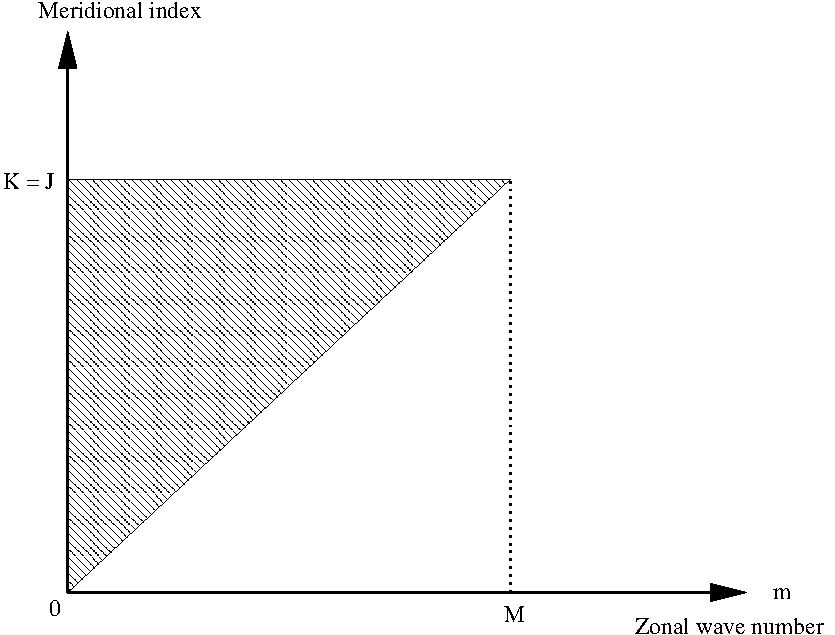
\includegraphics[width=0.6\linewidth]{science/triangular.pdf}
\else
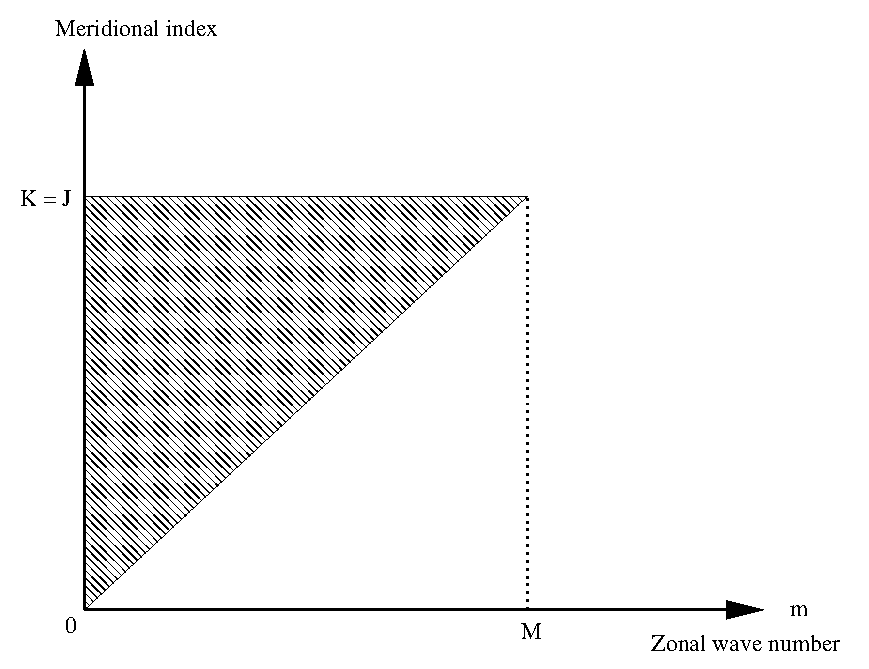
\includegraphics{science/triangular.eps}
\fi
\]
\caption{\label{fig:triangular}Triangular truncation}
\end{figure}

The triangular truncations are special cases of the pentagonal one in which
$M = J = K$.  

The summation limit, $N(m)$ is given by
\[
N = J+|m| \qquad \mbox{if} \qquad J+|m| \le K \qquad
\mbox{and} \qquad
N = K \qquad \mbox{if} \qquad J+|m| > K
\]

The standard truncations used in \echam{} are at wave numbers 31,
63, 127 or 255.

\clearpage

\subsubsection{Spectral/grid-point transforms, and the evaluation of 
               spectral tendencies} 

The general form of the equations follow that of the early multi-level
spectral models described by \cite{bourke74} and \cite{hoskins75},
although the present model differs in its use of an advective form for
the equations \ref{(2.2.17)}, \ref{(2.2.18)}, \ref{(2.2.3)}, and
\ref{(2.2.11)}. Equations for the corresponding spectral coefficients
are obtained by multiplying each side of these equations by
$P^m_n(\mu)\e{-im\lambda}$ and integrating over the sphere. This
yields, from \ref{(2.3.1.4)},

\begin{eqnarray}
\dnd{\xi^m_n}{t} & = & \frac{1}{4\pi a}\int\limits_{-1}^{1}
\int\limits_{0}^{2\pi}\left(\frac{1}{1-\mu^2}\dnd{(F_V+P_V)}{\lambda}
-\dnd{(F_U+P_U)}{\mu}\right)P^m_n(\mu)\e{-im\lambda}d\lambda d\mu\nonumber\\
&&+(K_{\xi})^m_n
\label{(2.3.2.1)}\\
\dnd{D^m_n}{t} & = & \frac{1}{4\pi a}\int\limits_{-1}^{1}
\int\limits_{0}^{2\pi}\left(\frac{1}{1-\mu^2}\dnd{(F_U+P_U)}{\lambda}
+\dnd{(F_V+P_V)}{\mu}\right)P^m_n(\mu)\e{-im\lambda}d\lambda d\mu\nonumber\\
&&-\frac{1}{4\pi}\int\limits_{-1}^{1}\int\limits_{0}^{2\pi}(\nabla^2G)P^m_n(\mu)\e{-im\lambda}d\lambda d\mu + (K_{D})^m_n
\label{(2.3.2.2)}\\
\dnd{T^m_n}{t} & = & \frac{1}{4\pi}\int\limits_{-1}^{1}
\int\limits_{0}^{2\pi}(F_T+P_T)P^m_n(\mu)\e{-im\lambda}d\lambda d\mu
+(K_{T})^m_n
\label{(2.3.2.3)}\\
\dnd{(\ln p_s)^m_n}{t} & = & \frac{1}{4\pi}\int\limits_{-1}^{1}
\int\limits_{0}^{2\pi}F_PP^m_n(\mu)\e{-im\lambda}d\lambda d\mu
\label{(2.3.2.6)}
\end{eqnarray}

where $F_U$, $F_V$ and $G$ are given by \ref{(2.2.19)} - \ref{(2.2.21)}, and\\

\begin{eqnarray}
F_T & = & -\frac{U}{a(1-\mu^2)}\dnd{T}{\lambda}-\frac{V}{a}\dnd{T}{\mu}
-\dot{\eta}\dnd{T}{\eta}+\frac{\kappa T_{\nu}\omega}{(1+(\delta-1)q_v)p}
\label{(2.3.2.7)}\\
F_P & = & -\frac{1}{p_s}\int\limits_{0}^{1}
\nabla\cdot(\vec{v}_h\dnd{p}{\eta})d\eta
\label{(2.3.2.10)}
\end{eqnarray}

Equations \ref{(2.3.2.3)} - \ref{(2.3.2.6)} are in the form used in the
model. The corresponding forms for the vorticity and divergence
equations are obtained from \ref{(2.3.2.1)} and \ref{(2.3.2.2)} by integration by parts and use of \ref{(2.3.1.13)}:

\begin{eqnarray}
\dnd{\xi^m_n}{t} & = & \frac{1}{4\pi a}\int\limits_{-1}^{1}
\int\limits_{0}^{2\pi}\frac{1}{1-\mu^2}[im(F_V+P_V)P^m_n(\mu)
-(F_U+P_U)H^m_n(\mu)]\e{-im\lambda}d\lambda d\mu\nonumber\\
&&+(K_{\xi})^m_n
\label{(2.3.2.11)}\\
\dnd{D^m_n}{t} & = & \frac{1}{4\pi a}\int\limits_{-1}^{1}
\int\limits_{0}^{2\pi}\frac{1}{1-\mu^2}[im(F_U+P_U)P^m_n(\mu)
+(F_V+P_V)H^m_n(\mu)]\e{-im\lambda}d\lambda d\mu\nonumber\\
&&+\frac{n(n+1)}{4\pi a^2}\int\limits_{0}^{1}
\int\limits_{0}^{2\pi}GP^m_n(\mu)\e{-im\lambda}d\lambda d\mu+(K_D)^m_n
\label{(2.3.2.12)}
\end{eqnarray}

where $H^m_n(\mu)$ is given by \ref{(2.3.1.20)}. 

An outline of the model's computation of spectral tendencies may now
be given. First, a grid of points covering the sphere is
defined. Using the basic definition of the spectral expansions
\ref{(2.3.1.1)} and equations \ref{(2.3.1.14)} - \ref{(2.3.1.19)},
values of $\xi$, $D$, $U$, $V$, $T$, and $\ln{p_s}$ are calculated at the
gridpoints, as are the derivatives

\begin{equation}
\dnd{T}{\lambda},\dnd{T}{\mu}, \dnd{\ln{p_s}}{\lambda} \mbox{and} \dnd{\ln{p_s}}{\mu}\nonumber
\end{equation}

using \ref{(2.3.1.9)}. The resulting gridpoint values are sufficient
to calculate gridpoint values of $F_U, F_V, F_T, F_p$ and $G$,
together with the parameterized tendencies $P_U, P_V$, and $P_T$, since
prognostic surface fields associated with the parameterization are
defined and updated on the same grid.  The integrands of the
prognostic equations \ref{(2.3.2.11)}, \ref{(2.3.2.12)},
\ref{(2.3.2.3)} - \ref{(2.3.2.6)} are thus known at each gridpoint,
and spectral tendencies are calculated by numerical quadrature.

The grid on which the calculations are performed is chosen to give an
exact (given the spectral truncation of the fields, and within
round-off error) contribution to spectral tendencies from quadratic
non-linear terms. The integrals with respect to $\lambda$ involve the
product of three trigonometric functions, and as shown by
\cite{machenhauer72} they may be evaluated exactly using a
regularly-spaced grid of at least $3\cdot M+1$ points. For the
latitudinal integrals, \cite{eliasen70} showed that quadratic
nonlinear terms lead to integrands which are polynomials in $\mu$ of a
certain order.

They may thus be computed exactly using Gaussian quadrature
(e.g. \cite{krylov62}, with points located at the (approximately
equally-spaced) latitudes which satisfy $P^0_{N_G}(\mu) = 0$, for
sufficiently large integer $N_G$. These latitudes form what are referred to
as the Gaussian latitudes.

In order to find the necessary number of Gaussian latitudes for the
triangular truncation, and from the exactness condition for the
Gaussian integration it may be shown that the number of Gaussian
latitudes $N_G$ must fulfil the following condition:

\begin{equation}
N_G\geq\frac{3\cdot K+1}{2} \nonumber
\end{equation}

The associated number of Gaussian latitudes with respect to the given
spectral resolution in \echam{}
%\footnote{Note: Since change of the ECMWF
%forecast model to the Semi-Lagrangian advection for the dynamics this
%model uses a linear truncation denoted $T_L$. This means that the
%number of Gaussian latitudes is smaller than in ECHAM5; e.g. $T_L$159
%has 160 latitudes and 320 langitudes while the spectral truncation
%corresponding to this grid-point resolution for ECHAM5 is T106.} 
is
given in table \ref{tab:Gaus}.

\begin{table}[htb]
\begin{center}
\begin{tabular}{ccc}\hline
Truncation & No. of Longitudes & No. of Latitudes \\ \hline
T31        &      96           &        48        \\
T63        &     192           &        96        \\ 
T127       &     384           &       192        \\
T255       &     768           &       384        \\ \hline
\end{tabular}
\end{center}
\caption[Truncation and associated number of Gaussian latitudes]{Truncation and associated number of Gaussian latitudes (and longitudinal number of gridpoints).\label{tab:Gaus}}   
\end{table}

An asymptotic property of the Legendre Functions which may be derived
directly from the definition \ref{(2.3.1.2)} is

\begin{equation}
P^m_n(\mu) \sim (1 - \mu^2)^{m/2} \; \mbox{as} \; (\mu\rightarrow\pm1).\nonumber
\end{equation}

Thus for large $m$ the functions become vanishingly small as the poles are
approached, and the contributions to the integrals \ref{(2.3.2.1)} -
\ref{(2.3.2.6)} from polar regions become less than the unavoidable
round-off error for sufficiently large zonal wavenumbers.

\subsection{\label{sec:verdis}Vertical discretization} 

\subsubsection{The hybrid vertical representation} 

To represent the vertical variation of the dependent variables $\xi$,
$D$, and $T$ the atmosphere is divided into layers as illustrated in
table \ref{tab:vert}. These layers are defined by the pressures of the
interfaces between them (the "half levels"), and these pressures are
given by

\begin{equation}
p_{k+1/2} = A_{k+1/2} + B_{k+1/2} \;\; p_s
\label{(2.4.1.1)}
\end{equation}


for $k = 0,1,2\dots NLEV$. The $A_{k+1/2}$ and $B_{k+1/2}$ are constants 
whose values effectively define the vertical coordinate.
Necessary values are

\begin{equation}
A_{1/2} = B_{1/2} = A_{NLEV+1/2} = 0 \ \ \mbox{and} \ \ B_{NLEV+1/2} = 1
\label{(2.4.1.2)}
\end{equation}

The usual sigma coordinate is obtained as the special case

\begin{equation}
 A_{k+1/2} = 0 \ , \ k = 0,1,\ldots, NLEV
\label{(2.4.1.3)}
\end{equation}

This form of hybrid coordinate has been chosen because it is
particularly efficient from a computational viewpoint. It
also allows a simple direct control over the "flattening" of
coordinate surfaces as pressure decreases, since the $A's$ and $B's$ may
be determined by specifying the distribution of half-level
pressures for a typical sea-level surface pressure and for a
surface pressure typical of the lowest expected to be
attained in the model. Coordinate surfaces are surfaces of
constant pressure at levels where $B_{k+1/2} = 0$.

The prognostic variables $\xi, D, T$ and $q_i$ are represented by
their values at intermediate (full-level) pressures, $p_k$. Values for
$p_k$ are not explicitly required by the model's vertical
finite-difference scheme, which is described in the following section,
but they are required by parameterization schemes, in the creation of
initial data, and in the interpolation to pressure levels that forms
part of the post-processing. Alternative forms for $p_k$ have been
discussed by \cite{simmons81a} and \cite{simmons81b}. Little
sensitivity has been found, and the simple form

\begin{equation}
p_k = \frac{1}{2}(p_{k+1/2}+p_{k-1/2})
\label{(2.4.1.4)}
\end{equation}

has been adopted, where half-level values are as given by
\ref{(2.4.1.1)}. The explicit relationship between $p$ and $p_s$
defined for model half levels implicitly determines a vertical
coordinate $\eta$. The model formulation is in fact such that this
coordinate need not be known explicitly, as demonstrated in the
following section. However, it is computationally convenient to define
$\eta$ for the radiative parameterization and for the vertical
interpolation used in the post-processing. The half-level values are
given by

\begin{equation}
\eta_{k+1/2} = \frac{A_{k+1/2}}{p_0} + B_{k+1/2}
\label{(2.4.1.5)}
\end{equation}

where $p_0$ is constant pressure. From \ref{(2.4.1.1)} it is seen that
this coordinate is identical to the usual $\sigma$ when $A_{k+1/2}$ =
0, and in general equals $\sigma$ when $p_0=p_s\cdot \eta = p/p_0$ at
levels where coordinate surfaces are surfaces of constant
pressure. Values of $\eta$ between half-levels are given by linear
interpolation :

\begin{equation}
\eta = \eta_{k+1/2} + \frac{(p-p_{k+1/2})(\eta_{k+1/2}-\eta_{k-1/2})}
{(p_{k+1/2} - p_{k-1/2})} \ \ \mbox{for} \ \ p_{k-1/2} \leq p \leq p_{k+1/2}
\label{(2.4.1.6)}
\end{equation}

\echam{} is used with 47 and 95 levels. Both vertical grids share the
lowermost 12 layers as well as the uppermost layer centered at 1 Pa. The
top-of-the-model pressure is 0 Pa, thus the whole atmospheric mass is in
the model domain. The value of $p_0$ used for the definition of $\eta$ is
the reference sea-level pressure of 101325 Pa.
\newpage


%-----------------------------------------------------------------------------
\bottomcaption[Vertical-coordinate parameters]{Vertical-coordinate parameters of the 47- and 95-layer \echam{} model} \label{tab:vert}
\tablehead{\hline $k$ & $A_{k+\frac{1}{2}}\;[Pa]$ & $B_{k+\frac{1}{2}}$ & $A_{k+\frac{1}{2}}\;[Pa]$ & $B_{k+\frac{1}{2}}$ \\ \hline \hline}
%
\tabletail{\hline \hline \multicolumn{5}{|l|}{table \ref{tab:vert} to be continued $\ldots$} \\ \hline}
\tablelasttail{\hline \hline}
%-----------------------------------------------------------------------------
\xentrystretch{0.05}
\begin{center}
\begin{xtabular}{|r||rr||rr|}
 0 &     0.000000  & 0.0000000000 &        0.00000000 & 0.00000000 \\
 1 &     1.989185  & 0.0000000000 &        1.98918247 & 0.00000000 \\
 2 &     6.572090  & 0.0000000000 &        2.69261074 & 0.00000000 \\
 3 &    15.673903  & 0.0000000000 &        3.54616451 & 0.00000000 \\
 4 &    30.624279  & 0.0000000000 &        4.57676125 & 0.00000000 \\
 5 &    54.545720  & 0.0000000000 &        5.81494045 & 0.00000000 \\
 6 &    92.558830  & 0.0000000000 &        7.29508114 & 0.00000000 \\
 7 &   150.504697  & 0.0000000000 &        9.05558681 & 0.00000000 \\
 8 &   235.327458  & 0.0000000000 &       11.13899899 & 0.00000000 \\
 9 &   356.100259  & 0.0000000000 &       13.59204197 & 0.00000000 \\
10 &   523.919524  & 0.0000000000 &       16.46557617 & 0.00000000 \\
11 &   751.042942  & 0.0000000000 &       19.81443787 & 0.00000000 \\
12 &  1051.137225  & 0.0000000000 &       23.69715881 & 0.00000000 \\
13 &  1438.988411  & 0.0000000000 &       28.17553710 & 0.00000000 \\
14 &  1930.177360  & 0.0000000000 &       33.31410217 & 0.00000000 \\
15 &  2540.697000  & 0.0000000000 &       39.17933655 & 0.00000000 \\
16 &  3286.553000  & 0.0000000000 &       45.83877563 & 0.00000000 \\
17 &  4199.574000  & 0.0000000000 &       53.36004639 & 0.00000000 \\
18 &  5303.957000  & 0.0000000000 &       61.84652710 & 0.00000000 \\
19 &  6624.704000  & 0.0000000000 &       71.41293335 & 0.00000000 \\
20 &  8187.185000  & 0.0000000000 &       82.18634033 & 0.00000000 \\
21 &  9976.137000  & 0.0004000000 &       94.30740356 & 0.00000000 \\
22 & 11820.540000  & 0.0029000000 &      107.93159485 & 0.00000000 \\
23 & 13431.390000  & 0.0092000000 &      123.23060608 & 0.00000000 \\
24 & 14736.360000  & 0.0203000000 &      140.39379883 & 0.00000000 \\
25 & 15689.210000  & 0.0370000000 &      159.62977600 & 0.00000000 \\
26 & 16266.610000  & 0.0595000000 &      181.16809082 & 0.00000000 \\
27 & 16465.000000  & 0.0879000000 &      205.26101685 & 0.00000000 \\
28 & 16297.620000  & 0.1220000000 &      232.18553162 & 0.00000000 \\
29 & 15791.600000  & 0.1614000000 &      262.24536133 & 0.00000000 \\
30 & 14985.270000  & 0.2057000000 &      295.77294922 & 0.00000000 \\
31 & 13925.520000  & 0.2542000000 &      333.13256836 & 0.00000000 \\
32 & 12665.290000  & 0.3062000000 &      374.72143555 & 0.00000000 \\
33 & 11261.230000  & 0.3611000000 &      420.97338867 & 0.00000000 \\
34 &  9771.406000  & 0.4182000000 &      472.36132813 & 0.00000000 \\
35 &  8253.211000  & 0.4767000000 &      529.40039063 & 0.00000000 \\ 
36 &  6761.340000  & 0.5359000000 &      592.64990234 & 0.00000000 \\
37 &  5345.914000  & 0.5951000000 &      662.71801758 & 0.00000000 \\
38 &  4050.718000  & 0.6536000000 &      740.26416016 & 0.00000000 \\
39 &  2911.569000  & 0.7106000000 &      826.00268555 & 0.00000000 \\
40 &  1954.805000  & 0.7654000000 &      920.70605468 & 0.00000000 \\
41 &  1195.890000  & 0.8172000000 &     1025.20947265 & 0.00000000 \\
42 &   638.148900  & 0.8650000000 &     1140.41430664 & 0.00000000 \\
43 &   271.626500  & 0.9077000000 &     1267.29199218 & 0.00000000 \\
44 &    72.063600  & 0.9442000000 &     1406.88818359 & 0.00000000 \\
45 &     0.000000  & 0.9730000000 &     1560.32666016 & 0.00000000 \\
46 &     0.000000  & 0.9923000000 &     1728.81445313 & 0.00000000 \\
47 &     0.000000  & 1.0000000000 &     1913.64550781 & 0.00000000 \\
48 &               &              &     2116.40527343 & 0.00000000 \\
49 &               &              &     2338.83251953 & 0.00000000 \\
50 &               &              &     2582.83544922 & 0.00000000 \\
51 &               &              &     2850.50659180 & 0.00000000 \\
52 &               &              &     3144.14184570 & 0.00000000 \\
53 &               &              &     3466.25976563 & 0.00000000 \\
54 &               &              &     3819.62304688 & 0.00000000 \\
55 &               &              &     4207.26171875 & 0.00000000 \\
56 &               &              &     4632.50390625 & 0.00000000 \\
57 &               &              &     5098.99218750 & 0.00000000 \\
58 &               &              &     5610.73046875 & 0.00000000 \\
59 &               &              &     6172.44531250 & 0.00000000 \\
60 &               &              &     6789.26171875 & 0.00000000 \\
61 &               &              &     7464.85546875 & 0.00000000 \\
62 &               &              &     8205.07421875 & 0.00000000 \\
63 &               &              &     9013.73437500 & 0.00004644 \\
64 &               &              &     9876.25000000 & 0.00034244 \\
65 &               &              &    10779.67968750 & 0.00110447 \\
66 &               &              &    11698.04296875 & 0.00262147 \\
67 &               &              &    12606.03906250 & 0.00530741 \\
68 &               &              &    13479.76171875 & 0.00948636 \\
69 &               &              &    14289.19140625 & 0.01555587 \\
70 &               &              &    15005.62109375 & 0.02390020 \\
71 &               &              &    15604.63671875 & 0.03493614 \\
72 &               &              &    16062.08593750 & 0.04900495 \\
73 &               &              &    16355.96484375 & 0.06649876 \\
74 &               &              &    16464.95703125 & 0.08780068 \\
75 &               &              &    16370.24609375 & 0.11324221 \\
76 &               &              &    16058.29296875 & 0.14307529 \\
77 &               &              &    15520.17968750 & 0.17757314 \\
78 &               &              &    14753.79296875 & 0.21690041 \\
79 &               &              &    13765.30859375 & 0.26105165 \\
80 &               &              &    12573.00000000 & 0.30987769 \\
81 &               &              &    11218.07421875 & 0.36276281 \\
82 &               &              &     9756.42187500 & 0.41877347 \\
83 &               &              &     8253.21093750 & 0.47670001 \\
84 &               &              &     6761.33984375 & 0.53590000 \\
85 &               &              &     5345.91406250 & 0.59509999 \\
86 &               &              &     4050.71801758 & 0.65359998 \\
87 &               &              &     2911.56909180 & 0.71060002 \\
88 &               &              &     1954.80493164 & 0.76539999 \\
89 &               &              &     1195.88989258 & 0.81720001 \\
90 &               &              &      638.14892578 & 0.86500001 \\
91 &               &              &      271.62646484 & 0.90770000 \\
92 &               &              &       72.06359863 & 0.94419998 \\
93 &               &              &        0.00000000 & 0.97299999 \\
94 &               &              &        0.00000000 & 0.99229997 \\
95 &               &              &        0.00000000 & 1.00000000 \\ 
\end{xtabular}
\end{center}
\xentrystretch{0.1}
\newpage


























\subsubsection{The vertical finite-difference scheme} 

The vertical finite-difference scheme is a generalization to the
hybrid coordinate with form \ref{(2.4.1.1)} of the scheme adopted in
the first operational ECMWF model \cite[]{burridge77}, apart from a
small modification concerned with the conservation of angular
momentum. The generalized scheme has been discussed by
\cite{simmons81a} and \cite{simmons81b}, and the presentation here is
restricted to a prescription of the finite-difference forms of the
various terms of the continuous equations that involve $\eta$.

\subsubsection{The surface-pressure tendency}

The finite-difference analogue of \ref{(2.2.11)} is

\begin{equation}
\dnd{\ln{p_s}}{t} = -\frac{1}{p_s}\sum\limits^{NLEV}_{k=1}
\nabla \cdot (\vec{v}_k\Delta p_k)
\label{(2.4.2.1)}
\end{equation}

where the subscript $k$ denotes a value for the $k$-th layer, and

\begin{equation}
\Delta p_k = p_{k+1/2}-p_{k-1/2}
\label{(2.4.2.2)}
\end{equation}

From \ref{(2.4.1.1)} we obtain

\begin{equation}
\dnd{\ln{p_s}}{t} = -\sum\limits^{NLEV}_{k=1}\left\{\frac{1}{p_s} D_k\Delta p_k
+ (\vec{v}_k \cdot \nabla \ln p_s) \Delta B_k\right\}
\label{(2.4.2.3)}
\end{equation}

   where

\begin{equation}
\Delta B_k = B_{k+1/2}-B_{k-1/2}
\label{(2.4.2.4)}
\end{equation}

\subsubsection{The continuity equation}

Equation \ref{(2.2.10)} gives

\begin{equation}
\left(\dot{\eta}\dnd{p}{\eta}\right)_{k+1/2} = -\dnd{p_{k+1/2}}{t} 
-\sum\limits^{k}_{j=1}\nabla \cdot (\vec{v}_j \Delta p_j)
\label{(2.4.2.5)}
\end{equation}

 and from \ref{(2.4.1.1)}

\begin{equation}
\left(\dot{\eta}\dnd{p}{\eta}\right)_{k+1/2} = -p_s\left[B_{k+1/2}\dnd{\ln{p_s}}{t}
+ \sum\limits^{k}_{j=1} \left\{\frac{1}{p_s} D_j\Delta p_j
+ (\vec{v}_j \cdot \nabla \ln p_s) \Delta B_j\right\}\right]
\label{(2.4.2.6)}
\end{equation}

where $\dnd{\ln{p_s}}{t}$ is given by \ref{(2.4.2.3)}.

\subsubsection{Vertical advection}

Given $\left(\dot{\eta}\dnd{p}{\eta}\right)_{k+1/2}$ computed from
\ref{(2.4.2.6)}, vertical advection of a variable is given by

\begin{equation}
\left(\dot{\eta}\dnd{X}{\eta}\right)_k = \frac{1}{2\Delta p_k} 
\left\{\left(\dot{\eta}\dnd{p}{\eta}\right)_{k+1/2}(X_{k+1}-X_k) 
+\left(\dot{\eta}\dnd{X}{\eta}\right)_{k-1/2}\cdot (X_k-X_{k-1})\right\}
\label{(2.4.2.7)}
\end{equation}

This form ensures that there is no spurious source or sink of kinetic
and potential energy due to the finite-difference representation of
vertical advection.

\subsubsection{The hydrostatic equation}
 
The form chosen for the finite-difference
analogue of \ref{(2.2.7)} is


\begin{equation}
\Phi_{k+1/2}-\Phi_{k-1/2} = -R_d\cdot (T_v)_k
\cdot \ln{\left(\frac{p_{k+1/2}}{p_{k-1/2}}\right)}
\label{(2.4.2.8)}
\end{equation}

which gives

\begin{equation}
\Phi_{k+1/2} = \Phi_S + \sum\limits^{NLEV}_{j=k+1}R_d\cdot (T_v)_j
\cdot \ln {\left(\frac{p_{j+1/2}}{p_{j-1/2}}\right)}
\label{(2.4.2.9)}
\end{equation}

Full level values of geopotential are given by

\begin{equation}
\Phi_k = \Phi_{k+1/2} + \alpha_k\cdot R_d\cdot (T_v)_k\ ,
\label{(2.4.2.10)}
\end{equation}

where

\begin{equation}
 \alpha_1 = \ln 2
\label{(2.4.2.11)}
\end{equation}

 and, for $k > 1$,

\begin{equation}
\alpha_k = 1 - \frac{p_{k-1/2}}{\Delta p_k}
\cdot \ln {\left(\frac{p_{k+1/2}}{p_{k-1/2}}\right)}
\label{(2.4.2.12)}
\end{equation}

Reasons for this particular choice of the $\alpha_k$ are given
below. 

\subsubsection{The pressure gradient term}

It is shown by \cite{simmons81b} that if the geopotential is given by
\ref{(2.4.2.10)}, the form

\begin{equation}
R_d\cdot (T_v\cdot\nabla\ln p)_k = \frac{R_d\cdot (T_v)_k}
{\Delta p_k}\left\{\left(\ln{\frac{p_{k+1/2}}{p_{k-1/2}}}\right)
\cdot \nabla p_{k-1/2} + \alpha_k\cdot\nabla(\Delta p_k)\right\}
\label{(2.4.2.13)}
\end{equation}

for the pressure-gradient term ensures no spurious source or sink of
angular momentum due to vertical differencing. This expression is
adopted in the model, but with the $\alpha_k$ given by
\ref{(2.4.2.12)} for all $k$. This ensures that the pressure-gradient
term reduces to the familiar form $R_d(T_v)_k\nabla\ln p_s$ in the
case of sigma coordinates, and the angular momentum conserving
property of the scheme still holds in the case in which the first
half-level below $p = 0$ is a surface of constant pressure. The choice
$\alpha_1 = 1$ in the hydrostatic equation would have given angular
momentum conservation in general, but a geopotential $\Phi_1$
inappropriate to the pressure-level $p = p_1 = \Delta p/2$. If,
alternatively, $\Phi_1$ were to be interpreted not as a value for a
particular level, but rather the mass-weighted layer-mean value, then
the choice $\alpha_1$ would be appropriate.

It is shown by \cite{simmons91} that the form \ref{(2.4.2.13)} can be
significantly improved, with benefit particularly in regions of steep
terrain, if $T_v$ is replaced by its deviation from a reference state,

\begin{equation}
\tilde{T}_v = T_v - T_0 \left(\frac{p}{p_0}\right)^{\beta}
\label{(2.4.2.14)}
\end{equation}

where $\beta = \gamma \cdot \frac{R_d}{g}$, $p_0 = 1013.25$ hPa, $T_0
= 288$ K and $\gamma = 6.5$ K/km. The reference temperature
\ref{(2.4.2.14)} is based on the tropospheric part of the
\cite{icao64} standard atmosphere with a uniform lapse rate $\gamma$.

Using the form \ref{(2.4.1.1)} for the half-level pressures
\ref{(2.4.2.13)} may be written

\begin{equation}
R_d\cdot (\tilde{T}_v\cdot\nabla\ln p)_k = \frac{R_d\cdot (\tilde{T}_v)_k}
{\Delta p_k}\left\{\Delta B_k + C_k \cdot \frac{1}{\Delta p_k}
\cdot \left(\ln{\frac{p_{k+1/2}}{p_{k-1/2}}}\right)\right\} \nabla p_s
\label{(2.4.2.15)}
\end{equation}

where

\begin{equation}
C_k = A_{k+1/2} \cdot B_{k-1/2} - A_{k-1/2} \cdot B_{k+1/2}
\label{(2.4.2.16)}
\end{equation}

The modified form \ref{(2.4.2.15)} finally requires a reformulation of
the surface geopotential according to

\begin{equation}
\Phi_S = g \cdot z_S + \frac{R_d \cdot T_0}{\beta}
\cdot \left(\frac{p_s}{p_0}\right)^{\beta}
\label{(2.4.2.17)}
\end{equation}

\subsubsection{Energy-conversion term}

To obtain a form for the term $\kappa \cdot T_v
\cdot\omega / (1 + (\delta - 1)q_v)$ in \ref{(2.2.3)} we use
\ref{(2.2.8)} to write

\begin{equation}
\left(\frac{\kappa \cdot T_v \cdot\omega}{(1 + (\delta - 1)q_v)p}\right)_k 
= \frac{\kappa \cdot (T_v)_k}{1 + (\delta - 1)(q_v)_k}
\left(\frac{\omega}{p}\right)_k
\label{(2.4.2.18)}
\end{equation}

where

\begin{equation}
\left(\frac{\omega}{p}\right)_k = -\frac{1}{p}
\int\limits^{\eta_k}_{0}\nabla\cdot\left(\vec{v}\cdot\dnd{p}{\eta}\right)d\eta
+(\vec{v}\cdot\nabla\ln p)_k 
\label{(2.4.2.19)}
\end{equation}

An expression for $\left(\frac{\omega}{p}\right)_k$ is then determined 
by the requirement that the difference scheme conserves the total energy 
of the model atmosphere for adiabatic, frictionless motion. This is 
achieved by

\begin{itemize}

\item evaluating the first term on the right-hand side of \ref{(2.4.2.19)} by

\begin{equation}
-\frac{1}{\Delta p_k}\left\{\left(\ln{\frac{p_{k+1/2}}{p_{k-1/2}}}\right)
\cdot \sum\limits^{k-1}_{k=1}\nabla\cdot(\vec{v}_j\cdot\Delta p_j) 
+ \alpha_k \nabla\cdot (\vec{v}_k\cdot\Delta p_k)\right\}
\label{(2.4.2.20)}
\end{equation}

where the $\alpha_k$ are as given by \ref{(2.4.2.11)} and  \ref{(2.4.2.12)},
and as in  \ref{(2.4.2.3)} and  \ref{(2.4.2.5)}

\begin{equation}
\nabla\cdot (\vec{v}_k\cdot\Delta p_k) = D_k \cdot\Delta p_k
+ p_s\cdot (\vec{v}_k\cdot\nabla\ln p_s)\cdot\Delta B_k
\label{(2.4.2.21)}
\end{equation}

\item using the form of \ref{(2.4.2.15)} to evaluate the second term on the right-hand side of \ref{(2.4.2.19)}

\begin{equation}
(\vec{v}\cdot\nabla\ln p)_k = \frac{p_s}{\Delta p_k}
\cdot\left\{\Delta B_k + C_k \cdot \frac{1}{\Delta p_k}
\cdot \left(\ln{\frac{p_{k+1/2}}{p_{k-1/2}}}\right)\right\}
\cdot\vec{v}_k\cdot\nabla\ln p_s
\label{(2.4.2.22)}
\end{equation}
\end{itemize}

\subsection{Time integration scheme} 

A semi-implicit time scheme is used for equations of divergence,
temperature and surface pressure, based on the work of
\cite{robert72}. The growth of spurious computational modes is
inhibited by a time filter \cite[]{asselin72}. In addition, a
semi-implicit method for the zonal advection terms in the vorticity
equation is used, following results obtained by
\cite{robert81,robert82}. He showed that in a semi-implicit shallow
water equation model the time-step criterion was determined by the
explicit treatment of the vorticity equation. Facilities also exist
for selective damping of short model scales to allow use of longer
timesteps. 
These are incorporated within the horizontal diffusion.
The semi-implicit schemes are formally given by:


\begin{eqnarray}
\delta_t\xi & = & ZT -\frac{1}{2a}\beta_{Z}\frac{U_r(\mu)}{1-\mu^2}
\dnd{\Delta_{tt}\xi}{\lambda}
\label{(2.5.1)}\\
\delta_tD & = & DT - \nabla^2G -\frac{1}{2}\beta_{DT}\nabla^2
\{\gamma\delta_{tt}T + R_dT_r\Delta_{tt}\ln{p_s}\}
\label{(2.5.4)}\\
\delta_tT & = &  TT -\frac{1}{2}\beta_{DT}\tau
\Delta_{tt}D
\label{(2.5.5)}\\
\delta_t\ln{p_s} & = &  PT -\frac{1}{2}\beta_{DT}\nu
\Delta_{tt}D
\label{(2.5.6)}
\end{eqnarray}

Here the terms $ZT, DT, G, TT$ and $PT$ represent those on the
right-hand sides of equations \ref{(2.2.17)}, \ref{(2.2.18)},
\ref{(2.2.3)} and \ref{(2.2.11)}, apart from the diffusion terms,
which are neglected here. Adiabatic components are evaluated at the
current time, $t$, and parameterized components are generally evaluated
using values of fields at the previous timestep, $t-\Delta t$.
%The treatment of diffusion terms is described in section \ref{sec:hordif}.

The remaining terms on the right-hand sides of \ref{(2.5.1)} - \ref{(2.5.6)}
 are corrections associated with the semi-implicit time schemes, and are
discussed in more detail below. The operators $\delta_t$ and $\Delta_{tt}$ 
are given by

\begin{eqnarray}
\delta_tX & = & \frac{(X^+ - X^-_f)}{2\Delta t}
\label{(2.5.7)}\\
\Delta_{tt}X & = & X^+ + X^-_f - 2X
\label{(2.5.8)}
\end{eqnarray}

where $X$ represents the value of a variable at time $t$, $X^+$ the value
at time  $t + \Delta t$, and $X^-_f$ a filtered value at time  $t - \Delta t$.
 A further operator that will be used is

% PAGE 24

\begin{equation}
\tilde\Delta_{tt}X = X^-_f - 2X
\label{(2.5.9)}
\end{equation}

The time filtering is defined by

\begin{equation}
X_f = X + \epsilon _f (X^-_f - 2X + X^+)
\label{(2.5.10)}
\end{equation}

and it is computationally convenient to split it into two parts;


\begin{eqnarray}
\tilde X_f & = & X + \epsilon _f (X^-_f - 2X)
\label{(2.5.11)}\\
X_f & = & \tilde X_f + \epsilon _f X^+
\label{(2.5.12)}
\end{eqnarray}

The timestep $\Delta t$ depends on resolution, while $\epsilon _f =
0.1$ is independent of the resolution.

\subsubsection{The semi-implicit treatment of vorticity\label{sec:timdis}}

Referring to equation \ref{(2.5.1)}, an explicit treatment of the
vorticity equation is obtained by setting $\beta_{Z} = 0$. Otherwise
$\beta_{Z} = 1$ and $U_r(\mu)$ is a zonally-uniform reference zonal
velocity, multiplied by $\cos \theta$. Terms describing advection by
this reference velocity are represented implicitly by the arithmetic
mean of values at times $t+\Delta t$ and $t-\Delta t$, while the
remainder of the tendencies are represented explicitly by values at
time $t$.  $U_r(\mu)$ may vary in the vertical.

For the vorticity equation, \ref{(2.2.17)} is used to write

\begin{equation}
ZT = \frac{1}{\alpha (1-\mu^2)}\dnd{(F_V+P_V)}{\lambda}
- \frac{1}{a}\dnd{(F_U+P_U)}{\mu}
\label{(2.5.19)}
\end{equation}

where the horizontal diffusion term has for convenience been
neglected. Transforming into Fourier space gives:


\begin{equation}
\xi^+_m = b_m (\mu) = \left[\left(\xi^-_f + \frac{2 \ im \Delta t}
{a(1-\mu^2)}(F_V+P_V)\right)_m 
- 2  \ im \Delta t \alpha (\mu)\tilde \Delta_{tt}\xi_m
- \frac{2 \Delta t}{a}\dnd{(F_U+P_U)_m}{\mu}\right]
\label{(2.5.20)}
\end{equation}

The factor $b_m (\mu)$ renders the right-hand side of this equation
unsuitable for direct integration by parts, but a suitable
form is found from the relation

\begin{equation}
b_m (\mu) \dnd{(F_U+P_U)}{\mu} = \dnd{\{b_m (\mu)(F_U+P_U)\}}{\mu}
- c_m (\mu)(F_U+P_U)
\label{(2.5.21)}
\end{equation}

where

\begin{equation}
c_m (\mu) = \dnd{\{b_m (\mu)\}}{\mu}
\label{(2.5.22)}
\end{equation}

This gives

\begin{equation}
\xi^+_m = \tilde{Z}_{\lambda m} (\mu) + \dnd{\tilde{Z}_{\mu m} (\mu)}{\mu}
\label{(2.5.23)}
\end{equation}

where

\begin{equation}
\tilde{Z}_{\lambda m} (\mu) = b_m (\mu) (\xi^-_f)_m\nonumber
+   2 \Delta t  \left(imb_m(\mu)\left[\frac{(F_V+P_V)_m}{a(1-\mu^2)}
- \alpha (\mu)\tilde \Delta_{tt}\xi_m\right]
 + \frac{1}{a}c_m(\mu)(F_U+P_U)_m\right)
\label{(2.5.24)}
\end{equation}

and

\begin{equation}
\tilde{Z}_{\lambda m} (\mu) = -\frac{2 \Delta t}{a}b_m (\mu) (F_U+P_U)_m
\label{(2.5.25)}
\end{equation}

New values $(\xi^m_n)^+$ are obtained from \ref{(2.5.23)} by Gaussian
quadrature,
         using integration by parts as illustrated by \ref{(2.3.2.1)} and
         \ref{(2.3.2.11)} for the continuous form of the equations.


$U_r(\mu)$ is the arithmetic mean of the maximum and minimum
velocities multiplied by $cos\theta$, as computed for each latitude
and model level at timestep $t-\Delta t$. Different values are thus
used for different levels. In ECHAM5, $\beta_{Z}$ = 1 is used.

\subsubsection{The semi-implicit treatment of divergence, temperature and surface
            pressure}

Referring to equations \ref{(2.5.4)} - \ref{(2.5.6)}, an explicit
treatment of the divergence, temperature and surface pressure
equations is obtained by setting $\beta_{DT}$ = 0. For $\beta_{Z}$ =
1, the nature of the semi-implicit correction is such that gravity
wave terms for small amplitude motion about a basic state with
isothermal temperatue $T_r$ and surface pressure $p_r$ are treated
implicitly by the arithmetic mean of values at times $t+\Delta t$ and
$t-\Delta t$, while the remainder of tendencies are represented
explicitly by values at time $t$. The choice of an isothermal
reference temperature is governed by considerations of the stability
of the semi-implicit time scheme \cite[]{simmons78}, while the
appropriate choice of $p_r$ for the hybrid vertical coordinate is
discussed by \cite{simmons81a} and \cite{simmons81b}.

$\gamma,  \tau$ and $\nu$ in equations \ref{(2.5.4)} - \ref{(2.5.6)}
are operators obtained from linearizing the finite-difference forms
specified in section \ref{sec:verdis} about the reference state $(T_r,
\ p_r)$. Their definitions are


\begin{eqnarray}
(\gamma T)_k  & = & \alpha_k^rR_dT_k 
+ \sum\limits^{NLEV}_{j=k+1}R_dT_j \ln \left(
\frac{p^r_{j+1/2}}{p^r_{j-1/2}}\right)
\label{(2.5.26)}\\
(\tau D)_k  & = & \kappa T_r\left\{\frac{1}{\Delta p^r_k} \ln \left(
\frac{p^r_{j+1/2}}{p^r_{j-1/2}}\right)S^r_{k-1/2} + \alpha^r_kD_k\right\}
\label{(2.5.27)}
\end{eqnarray}

and

\begin{equation}
\nu D = \frac{S^r_{NLEV+1/2}}{p^r}
\label{(2.5.28)}
\end{equation}

where

\begin{eqnarray}
p^r_{k+1/2} & = & A_{k+1/2} + p_rB_{k+1/2}\nonumber\\
\Delta p^r_k & = & p^r_{k+1/2} - p^r_{k-1/2}
\label{(2.5.29)}\\
S^r_{k+1/2} & = & \sum\limits^{k}_{j=1}D_j\Delta p^r_j\nonumber
\end{eqnarray}

and the $\alpha_k^r$ are defined by \ref{(2.4.2.11)} and \ref{(2.4.2.12)} , but with half-level
pressures replaced by reference values $p^r_{k+1/2}$.

Expanding \ref{(2.5.4)} - \ref{(2.5.6)} using \ref{(2.5.7)} and \ref{(2.5.8)}, and writing $l$ to
denote $\ln p'_S$, we obtain

\begin{eqnarray}
D^+ & = & D^-_f + 2\Delta t (DT) - 2\Delta t \nabla^2 
          \{G + \frac{\beta_{DT}}{2} [\gamma(T^+ + T^-_f - 2T) \nonumber \\
    &   & + R_dT_r(l^+ + l^-_f - 2l)]\}
\label{(2.5.30)}\\
T^+ & = & T_1 - \Delta t \beta_{DT} \tau D^+
\label{(2.5.31)}
\end{eqnarray}

and

\begin{equation}
l^+ = l_1 - \Delta t \beta_{DT} \nu D^+
\label{(2.5.32)}
\end{equation}

where


\begin{equation}
T_1 = T^-_f + 2\Delta t (TT) - \Delta t \beta_{DT} \tau \tilde\Delta_{tt}D
\label{(2.5.33)}
\end{equation}

and

\begin{equation}
l_1 = l^-_f + 2\Delta t (PT) - \Delta t \beta_{DT} \nu \tilde\Delta_{tt}D
\label{(2.5.34)}
\end{equation}

Substituting \ref{(2.5.31)} and \ref{(2.5.32)} into \ref{(2.5.30)} then gives

\begin{equation}
(1 - \Gamma\nabla^2) D^+ = DT'
\label{(2.5.35)}
\end{equation}

where

\begin{eqnarray}
\Gamma & = & (\beta_{DT})^2(\Delta t)^2 (\gamma\tau +  R_dT_r\nu)
\label{(2.5.36)}\\
DT' & = & D^-_f + 2\Delta t(DT) + \nabla^2 R = \tilde{D}_{\lambda}
+ \tilde{D}_{\mu} + \nabla^2 R
\label{(2.5.37)}
\end{eqnarray}

with

\begin{eqnarray}
\tilde{D}_{\lambda} & = & D^-_f + \frac{2\Delta t}{a(1-\mu^2)}
\dnd{(F_U+P_U)}{\lambda}
\label{(2.5.38)}\\
\tilde{D}_{\mu} & = & \frac{2\Delta t}{a}
\dnd{(F_V+P_V)}{\mu}
\label{(2.5.39)}
\end{eqnarray}

and

\begin{equation}
R = - 2\Delta t\left\{G + \frac{B_{DT}}{2}
(\gamma T_2 + R_dT_rl_2)\right\}
\label{(2.5.40)}
\end{equation}

Here


\begin{eqnarray}
T_2 & = & T_1 + T^-_f - 2T
\label{(2.5.41)}\\
l_2 & = & l_1 + l^-_f - 2l
\label{(2.5.42)}
\end{eqnarray}

The sequence of these semi-implicit calculations in the model is thus
as follows. The expressions \ref{(2.5.33)}, \ref{(2.5.34)} and
\ref{(2.5.40)} - \ref{(2.5.42)} are computed on the Gaussian grid to
form the gridpoint values of $R$. The spectral expansion of $DT'$ is
then derived by Gaussian quadrature, using integration by parts as
illustrated by \ref{(2.3.2.2)} and \ref{(2.3.2.12)} for the continuous
form of the equations. Since

\begin{equation}
\{(1 - \Gamma \nabla^2) D^+ \}^m_n = \left(1+ 
\frac{n(n+1)}{a^2} \Gamma\right)(D^+)^m_n , 
\label{(2.5.43)}
\end{equation}

the spectral coefficients of divergence at time $t + \Delta t$ are
given from \ref{(2.3.2.2)} by

\begin{equation}
(D^+)^m_n =  \left(1+ \frac{n(n+1)}{a^2} \Gamma\right)^{-1}(DT')^m_n ,
\label{(2.5.44)}
\end{equation}

where this operation involves, for each $(m,n)$, multiplication of the
vector of $NLEV$ values of $(DT')^m_n$ by a pre-computed $NLEV\times
NLEV$ matrix whose elements are independent of time and determined by
writing the operators $\gamma , \ \tau$ and $\nu$ in matrix and vector
form. Finally, \ref{(2.5.31)} and \ref{(2.5.32)} are applied in
spectral space to compute spectral coefficients of $T$ and $\ln p'_S$
at time $t + \Delta t$ in terms of the spectral coefficients of $T_1$
and $l_1$ (again determined by Gaussian quadrature) and those of
$D^+$. In ECHAM5, $\beta_{DT}$ = 0.75, $T_r$ = 300 K and $p_r$ = 800 hPa.

\subsection{Nudging of dynamical variables}

The general circulation model \echam{} calculates the state of the
atmosphere starting at certain initial conditions and integrating over
time. The state of the atmosphere may be represented by a vector
$\vec{\xi}_t$ at a time $t\in\mathbb{R}_+$ in a 
certain abstract space $\mathbb{S}$. The state vector moves with time
in $\mathbb{S}$ and describes some trajectory. 
The trajectory $t\mapsto\vec{\xi}_t$ is unambiguously determined by the
initial and boundary conditions, and the model equations. However, even if two
initial states are very close to each other, the trajectories drift
apart with time and their mutual distance becomes larger than any
bound provided that we wait long enough. It is therefore impossible to
simulate any real historical trajectory $t\mapsto\vec{\zeta}_t$ even if the
initial state was 
set with all care because of the discretization errors in the
model. We cannot even expect that the trajectories remain close to
each other.   
If it is important for longer simulations to reproduce some
real historical trajectory $t\mapsto\vec{\zeta}_t$ at least in its
main characteristics, the 
``nudging'' technique can help to achieve this goal.
The idea is to use a relaxation mechanism that approaches the
simulated trajectory $t\mapsto\vec{\xi}_t$ to a given trajectory
$t\mapsto\vec{\zeta}_t$. 

Let $F: \mathbb{S}\rightarrow\mathbb{S}$ describe the time evolution of
$\vec{\xi}_t$ by the model equations without nudging:

\begin{equation}\label{eqintfree}
\frac{d}{dt}\vec{\xi}_t=F(\vec{\xi}_t).
\end{equation}

We add a relaxation term to this
equation that approaches $\vec{\xi}_t$ to $\vec{\zeta}_t$. To this
end, let $\boldsymbol{\kappa}:\mathbb{S}\rightarrow\mathbb{S}$ be a
(diagonal) matrix of relaxation coefficients and set:

\begin{equation}\label{eqdiffnudg}
\frac{d}{dt}\vec{\xi}_t=F(\vec{\xi}_t)-\boldsymbol{\kappa}(\vec{\xi}_t-\vec{\zeta}_t)
\end{equation}

If $\boldsymbol{\kappa}$ has small values, the ``nudging term''
$\boldsymbol{\kappa}(\vec{\xi}_t-\vec{\zeta}_t)$ does not influence
$\frac{d}{dt}\vec{\xi}_t$, but it dominates $F(\vec{\xi}_t)$ for large
values of $\boldsymbol{\kappa}$. Each matrix element of
$\boldsymbol{\kappa}$ can be interpreted as the inverse of a
corresponding relaxation time. Short relaxation times mean a dominant
nudging term, at longer relaxation times, the influence of nudging is
reduced. 

\echam{} provides two possibilities of solving differential
equation~(\ref{eqdiffnudg}): ({\it i\/}) an implicit method and ({\it
  ii\/}) an explicit 
method.

\subsubsection{Implicit nudging}\label{secnudgimpl}

The discretization of equation~(\ref{eqdiffnudg}) with respect to time
for implicit nudging is the following:

\begin{equation}\label{eqdiffnudgimpl}
\frac{\vec{\xi}_{t+\Delta t}-\vec{\xi}_{t}}{\Delta t}
= F(\vec{\xi}_{t+\Delta t})-\boldsymbol{\kappa}(\vec{\xi}_{t+\Delta
  t}-\vec{\zeta}_{t+\Delta t}) 
\end{equation}

In the above equation, $\Delta t$ is the integration time step. Some
authors like~\cite{kri913} set $2\Delta t$ instead because the integration
time step is two times longer than the time step in many time
integration schemes. 

Equation~(\ref{eqdiffnudgimpl}) could be solved using a similar
procedure as it is implemented for the solution of
equation~(\ref{eqintfree}) in \echam. The implicit form of
discretization of equation~(\ref{eqintfree})
can be written as
$(\vec{\xi}^\ast_{t+\Delta t}-\vec{\xi}_t)/\Delta
t=F(\vec{\xi}^\ast_{t+\Delta t})$ describing the integration from a
state $\vec{\xi}_t$ to a state $\vec{\xi}^\ast_{t+\Delta t}$ using the
model equation~(\ref{eqintfree}) without nudging. 
On the other hand, we may approximate
$F(\vec{\xi}_{t+\Delta t})$ in equation~(\ref{eqdiffnudgimpl}) by
$F(\vec{\xi}^\ast_{t+\Delta t})$ and 
get

\begin{displaymath}
\vec{\xi}_{t+\Delta t}-\vec{\xi}^\ast_{t+\Delta t} = - \Delta t
\boldsymbol{\kappa} (\vec{\xi}_{t+\Delta t}-\vec{\zeta}_{t+\Delta t})
\end{displaymath} 

Solving for $\vec{\xi}_{t+\Delta t}$ yields:

\begin{equation}\label{eqnudgimplvec}
\vec{\xi}_{t+\Delta t}=(1+\Delta t
\boldsymbol{\kappa})^{-1}(\vec{\xi}^\ast_{t+\Delta t}+\Delta t
\boldsymbol{\kappa}\vec{\zeta}_{t+\Delta t})
\end{equation}

or reformulated for any projection $\xi,\zeta$ on an arbitrary axis of
$\mathbb{S}$ representing e.g.~temperature or divergence of the wind
field and $\tau$ being the corresponding relaxation time
($\boldsymbol{\kappa}$ diagonal):

\begin{equation}\label{eqnumnimpl}
\xi_{t+\Delta t}=\frac{\tau}{\tau+\Delta t}\xi^\ast_{t+\Delta
  t}+\frac{\Delta t}{\tau+\Delta t}\zeta_{t+\Delta t}.
\end{equation}

The new $\xi_{t+\Delta t}$ is therefore a linear combination of the
prediction $\xi^\ast_{t+\Delta t}$ calculated with ``free'' \echam{}
and the nudging data 
$\zeta_{t+\Delta t}$ at that time. For small relaxation
times, we get

\begin{equation}\label{eqlimittau0impl}
\lim\limits_{\tau \rightarrow 0}\xi_{t+\Delta t}=\zeta_{t+\Delta t}.
\end{equation}

This means that we simply replace the original prediction by the
nudging data. For very large relaxation times, we get:

\begin{equation}\label{eqlimittauinfimpl}
\lim\limits_{\tau \rightarrow \infty}\xi_{t+\Delta
  t}=\lim\limits_{\tau\rightarrow\infty}\frac{1}{1+\Delta
  t/\tau}\xi^\ast_{t+\Delta t}=\xi^\ast_{t+\Delta t}.
\end{equation}

This means that the original prediction of free \echam{} is used
and the nudging 
data do not have any influence on the trajectory $t\mapsto\vec{\xi}_t$.

\subsubsection{Explicit nudging}\label{secnudgexpl}

The discretization of equation~(\ref{eqdiffnudg}) with respect to time
for explicit nudging is a bit different from its implicit form
(\ref{eqdiffnudgimpl}): 

\begin{equation}\label{eqdiffnudgexpl}
\frac{\vec{\xi}_{t+\Delta t}-\vec{\xi}_{t}}{\Delta t}
= F(\vec{\xi}_t)-\boldsymbol{\kappa}(\vec{\xi}_{t}-\vec{\zeta}_{t})
\end{equation}

From this follows with $(\vec{\xi}^\ast_{t+\Delta
  t}-\vec{\xi}_t)/\Delta t = F(\vec{\xi}_t)$:

\begin{displaymath}
\vec{\xi}_{t+\Delta t}=\vec{\xi}^\ast_{t+\Delta t}-\Delta t
\boldsymbol{\kappa} \left(\vec{\xi}_t-\vec{\zeta}_t\right)
\end{displaymath}

For small $\Delta t \boldsymbol{\kappa}$ (small time steps compared to
the relaxation times), one may approximate $\Delta t
\boldsymbol{\kappa}\vec{\xi}_t$ by $\Delta
t\boldsymbol{\kappa}\vec{\xi}^\ast_{t+\Delta t}$ leading to 

\begin{equation}
\vec{\xi}_{t+\Delta t}=(1-\Delta t
\boldsymbol{\kappa})\vec{\xi}^\ast_{t+\Delta t}+\Delta
t\boldsymbol{\kappa}\vec{\zeta}_t 
\end{equation}

This means for any projection:

\begin{equation}\label{eqnumnexpl}
\xi_{t+\Delta t}=\left(1-\frac{\Delta
    t}{\tau}\right)\xi^\ast_{t+\Delta t} + \frac{\Delta t}{\tau}\zeta_{t+\Delta t}
\end{equation}

Very long relaxation times~$\tau$ lead to the following
limit:

\begin{equation}\label{eqlimittauinfexpl}
\lim\limits_{\tau\rightarrow\infty}\xi_{t+\Delta t}=\xi^\ast_{t+\Delta t}
\end{equation}

We therefore just accept the original prediction of the time
integration and ignore the nudging data. On the other hand, very short
relaxation times show a wrong behaviour of
equation~(\ref{eqnumnexpl}):

\begin{equation}\label{eqlimittau0expl}
\lim\limits_{\tau\rightarrow 0}\xi_{t+\Delta t}=\xi^\ast_{t+\Delta
  t}+\left(\zeta_{t+\Delta t}-\xi^\ast_{t+\Delta
t}\right)\lim\limits_{\tau\rightarrow 0}\frac{\Delta
t}{\tau}={\rm sgn}\left(\zeta_{t+\Delta t}-\xi^\ast_{t+\Delta t}\right)\infty
\end{equation}

In general, the nudging equations (\ref{eqnumnimpl}) or
(\ref{eqnumnexpl}) are applied in spectral space to the logarithm of
the surface pressure, the 3--d temperature, and 3--d vorticity and
divergence of the wind field. For each model layer and variable, the
relaxation time can be set individually. There is also a possibility
to exclude spectral coefficients of certain order from the nudging
procedure. In general, the nudging mechanism is often used to reproduce
large scale dynamic phenomena as they are present in analysis data but
the boundary layer dynamics and 
local convection and diffusion processes are intended to be treated by
the parameterizations implemented in \echam. In such cases, the boundary
layer and higher order spectral coefficients should be excluded from
nudging. For a more detailed discussion of the choice of relaxation
times, see the article of~\cite{jeu969}.

In early versions of the nudging procedure, it was possible to nudge
the sea surface temperature also, but this leads to problems due to
hysteresis effects.


\section{Transport}

The flux form semi-Lagrangian scheme employed in ECHAM6 for passive
tracer transport has been introduced by \cite{lin96}.  This
type of advection scheme combines typical features of Eulerian, flux
form schemes (i.e., exact mass conservation to machine precision) with
the unconditional stability for all Courant numbers typical of
standard (non conservative) semi-Lagrangian schemes. For Courant
numbers smaller than one, the Lin-Rood schemes reverts to a
multidimensional flux form scheme which takes properly into account
transverse fluxes, such as those developed by Colella, LeVeque,
Leonard and others (see references in \cite{lin96}).  In the constant
velocity case at Courant number smaller than one, it is in fact
identical with the Colella {\it Corner Transport Upwind} scheme.  The
scheme is described here for application to incompressible flows, its
generalization to compressible fluids is described in \cite{lin96}.

Consider the conservative formulation of passive  advection 
in an incompressible fluid

\begin{equation}
\frac {\partial Q}{\partial t} + \nabla \cdot ( {\bf v}Q) =0, 
\label{cons}
\end{equation}

where $Q$ is the tracer concentration and the continuity equation is
given by

\begin{equation}
\nabla \cdot  {\bf v} =0.
\label{cont}
\end{equation}

It is to be remarked that there is an inherent coupling of
(\ref{cons}) to the continuity equation, since in the case of constant
tracer concentration (\ref{cons}) reduces to (\ref{cont}). This
property should be also guaranteed by the discretization of
(\ref{cons}).


Assuming a C-type grid staggering in which normal velocity components
are defined at the grid sides and scalar quantities (to be interpreted
as cell averages) are defined at the cell center, a flux form
discretization of (\ref{cons}) is given by


\begin{equation}
Q_{i,j}^{n+1} = Q_{i,j}^{n} 
- \Big ( {\cal X}_{i+\frac 12,j} -{\cal X}_{i-\frac 12,j} \Big ) 
-\Big (  {\cal Y}_{i,j+\frac 12} -{\cal Y}_{i,j-\frac 12} \Big )
\label{disc1}
\end{equation}

where ${\cal X}_{i+\frac 12,j} {\cal Y}_{i,j+\frac 12}$ and ${\cal
X}_{i-\frac 12,j} {\cal Y}_{i,j-\frac 12}$ are approximations of the
$Q$ fluxes in the E-W and N-S directions, respectively, integrated in
time over the time step $\Delta t .$ In order to achieve unconditional
stability, in the Lin-Rood scheme the fluxes are computed as the sum
of an {\it integer } and a {\it fractional} flux $$ {\cal X}_{i-\frac
12,j}={\cal X}^{int}_{i-\frac 12,j}+{\cal X}^{fr}_{i-\frac 12,j} .$$
The integer fluxes represent the contribution to the flux that arises
in case of Courant numbers larger than one at the cell side $i-\frac
12.$ More specifically, defining $$ C^x_{i-\frac 12,j}=\frac{\Delta t
u^{n+\frac 12}_{i-\frac 12,j}}{\Delta x}= K^x_{i-\frac
12,j}+c^x_{i-\frac 12,j}
$$

$$ 
K^x_{i-\frac 12,j}=INT(C^x_{i-\frac 12,j})  \ \ \ \ \ \ \ \ \
I=INT(i - C^x_{i-\frac 12,j})
$$
(where $INT$ has the same meaning as the corresponding
{\it Fortran95} intrinsic function) 
and assuming e.g. a positive velocity, the integer flux is defined 
as $${\cal X}^{int}_{i-\frac 12,j}=\sum_{k=1}^{K^x_{i-\frac 12,j}}Q^n_{i-k,j}. $$

Thus, the integer flux represents the mass transport through all the
cells crossed completely by a Lagrangian trajectory ending at
$(i-\frac 12,j)$ at timestep $n+1$ during a time interval $\Delta t.$

The fractional flux is defined as the Van Leer flux  

\begin{equation}
{\cal X}^{fr}_{i-\frac 12,j}= 
c^x_{i-\frac 12,j}\Bigg [Q^g_{I,j} 
+\frac{ Q^g_{I+1,j}-Q^g_{I-1,j} }4    
\Big ( SIGN(1,c^x_{i-\frac 12,j}) -c^x_{i-\frac 12,j} \Big ) \Bigg ]
\label{disc2}
\end{equation}

where $SIGN$ has the same meaning as the corresponding {\it Fortran95}
intrinsic function.

The intermediate value $Q^g_{i,j}$ used in the computation of the Van
Leer flux can be interpreted as a first order finite difference
approximation of
 
$$
\frac{\partial Q}{\partial t} +v\frac{\partial Q}{\partial y}=0,
$$

advanced in time $\Delta t / 2$ from timestep $ n $ along the
Lagrangian trajectory ending at $(i-\frac 12,j)$ at timestep $ n+1.$

More precisely,

$$
Q^g_{i,j} = \frac{ \Big (  Q^n_{i,J} +Q^n_{i,j}  \Big )}2
+\frac{\vert c^y_{i,j}\vert}2  \Big ( Q^n_{i,J^*} -Q^n_{i,J} \Big )
$$

where

$$
C^y_{i,j}=\frac{\Delta t}{2\Delta y}\Big ( v^{n+\frac 12}_{i,j-\frac 12}+v^{n+\frac 12}_{i,j+\frac 12}
\Big )
$$

$$
c^y_{i,j}= C^y_{i,j} - INT(C^y_{i,j}) \ \ \ \ \  J=j-INT(C^y_{i,j}) \ \ \ \ \ 
J^*=J-SIGN(1,C^y_{i,j}).
$$

The Lin and Rood scheme satisfies some fundamental requirements
for a tracer advection algorithm:

\begin{itemize}

\item mass conservation: by construction, since it is formulated in
flux form;

\item consistency with the discretization of the continuity equation:
setting $q=1$ yields a discretization  of (\ref{cont}) by the same scheme,

\item monotonicity of the 1D advection schemes: if a flux limiter is
applied to the centered difference $ Q^g_{I+1,j}-Q^g_{I-1,j} $ in
(\ref{disc2}) (see references in \cite{lin96}), the one dimensional flux
operators are guaranteed to be monotonic, although this in general
does not ensure that the full multidimensional scheme is monotonic as
well;

\item preservation of linear tracer correlations: if $q_1, q_2$ are
the concentrations of two different tracers such that $q^n_2=\alpha
q^n_1 + \beta, $ with $\alpha, \beta $ two constants, then the values
$q^{n+1}_1, q^{n+1}_2$ obtained by time update with the Lin and Rood
scheme still satisfy $q^{n+1}_2=\alpha q^{n+1}_1 + \beta. $

\end{itemize}


\section{Horizontal diffusion\label{sec:hordif}}\label{c4}

Unlike the other physical parameterizations which are computed in grid 
point space, the horizontal diffusion can conveniently be formulated in 
spectral space. Moreover, the treatment of horizontal diffusion differs 
from that of the other processes in that it does not involve a physical 
model of subgrid-scale processes, but rather a numerically convenient form 
of scale selective diffusion with coefficients determined empirically to 
ensure a realistic behavior of the resolved scales. As in many other 
models, the horizontal diffusion tendency is expressed in the form of a 
hyper-Laplacian,

\begin{equation}
\dnd{\chi}{t}=-(-1)^qK_{\chi}\nabla^{2q}\chi	
\label{4.1}
\end{equation}

where $\chi$ is vorticity, divergence or temperature (no horizontal
diffusion is applied to water components or trace constituents),
$K_{\chi}$ is a constant diffusion coefficient for the respective
variable, and $q > 0$ is an integer. The time rate of change of
spectral component $\chi_{n}$ is given by

\begin{equation}
\dnd{\chi_{n}}{t}=-K_{\chi}\left \{n(n+1)a^{-2}\right\}^q\chi_{n}	
\label{4.2}	
\end{equation}

where $a$ is the Earth's radius and $n$ is wavenumber. For
convenience, $K_{\chi}$ can be replaced by the e-folding damping time
$\tau$ of the highest resolvable wavenumber $n_{0}$

\begin{equation}
\tau(n_{0})\equiv\tau_{0}=K_{\chi}^{-1}\left\{n_{0}(n_{0}+1)a^{-2}
	\right\}^{-q}
	\label{4.3}
\end{equation}

so that \eref{4.2} can be expressed in terms of the order of the
scheme, $2q$, and damping time $\tau_{0}$. The scale selectivity of
the scheme increases with increasing $q$. Both damping time and order
depend on the horizontal resolution. Furthermore, in order to avoid
spurious wave reflection at the upper boundary of the model, the
diffusion is enhanced in the upper layers by gradually decreasing the
order of the scheme (Table \ref{t4.1}).

\setlength{\LTcapwidth}{\textwidth}
\setlength{\LTleft}{0pt}\setlength{\LTright}{0pt}

\begin{longtable}{c@{\extracolsep\fill}cccc}\hline\hline
\caption[Horizontal diffusion]{Damping time $\tau_{0}$ in hours (independent of model level) 
and order, $2q$, of horizontal diffusion scheme applied at different model 
levels}\\\hline\label{t4.1}
\endfirsthead
\caption[]{{\tt horizontal diffusion} --- continued}\\\hline
\endhead
\hline\multicolumn{5}{r}{\slshape table continued on next page}\\
\endfoot
\hline %\multicolumn{4}{r}{end of table}
\endlastfoot
Level&T31            & T63      & T127                     & T255\\
&($\tau_{0}=12$) &($\tau_{0}=7$) & ($\tau_{0}=1.5$)      &($\tau_{0}=0.5$)\\ 
\hline
\multicolumn{5}{c}{version with 47 levels}\\\hline
1--4 & 2 & 2 & --- & --- \\
5--7 & 4 & 4 & --- & --- \\
8--9 & 6 & 6 & --- & --- \\
10--11 & 8 & 8 & --- & ---\\
12--47 & 10 & 8 & --- & ---\\\hline
\multicolumn{5}{c}{version with 95 levels}\\\hline
1--10 & --- & 2 & 2 & 2 \\
11--20 & --- & 4 & 4 & 4 \\
21--25 & --- & 6 & 4 & 4 \\
26--95 & --- & 8 & 6 & 6\\\hline\hline
\end{longtable}



\newpage
\newcommand{\Iup}{I^{\uparrow}}
\newcommand{\Idn}{I^{\downarrow}}

\section{Radiative Transfer}

Beginning with ECHAM 6.2 radiative transfer is computed using PSrad \citep{pincus2013}, a two-stream model that descends from the RRTMG codes \citep{mlawer97,iacono2008} developed by Atmospheric and Environmental Research (AER). Irradiances are computed separately for the longwave and shortwave portions of the spectrum. Scattering is neglected in longwave calculations and sources internal to the atmosphere are neglected in shortwave calculations, both of which simplify the resulting equation sets. Spectral discretization is determined by the ``correlated-$k$'' method used to treat absorption by gases, so that upward and downward irradiances are calculated over a predetermined number of pseudo-wavelengths denoted by $\tilde{\nu}_g$. Below we describe the correlated-$k$ method and why it is adopted, the longwave and shortwave radiative transfer solvers, their required input data and how that is used to determine the radiative (or optical) properties of the atmosphere and surface, as well as details of the numerical implementation.

Below we adopt the radiance/irradiance terminology because it is shorter than referring to radiative intensity/flux.  The radiance at a point is a function of the incident angle of the radiative beam passing through that point, the irradiance is the sum of all beams (integral over angles in the hemisphere) that pass through a unit area.

\subsection{Spectral discretization: the correlated $k$ method for gaseous absorption}

The dynamical equations are sensitive to the divergence of broadband irradiances, with most of the radiant energy being carried in the wavelength interval ranging from 1 mm to 100 nm, and the break between the longwave and shortwave bands is roughly 4 microns.  Formally the broadband irradiance is defined by the intergral of the irradiance spectral density over the wavelengths of interest, so that if one is interested in wavelenghts $\lambda_1 < \nu \le \lambda_2$
\[
I = \int_{\lambda_1}^{\lambda_2} I_\lambda \mathrm{d}\lambda.
\]
This integral can be approximated by a sum over discrete frequencies, but because the spectral properties of the atmosphere vary strongly as a function of wavelength, with nearly singular line-like features at specific wavelengths, the required number of frequencies to well approximate the integral is prohibitively large given the balance between desired accuracy and computational resources.  

To address this shortcoming the spectrum is divided into bands, and within a band the band-averaged irradiance is approximated by a sum over a discrete set of pseudo wavelengths, $\tilde{\lambda}_{b,g},$ where we have chosen $b$ to index the band and $g$ to index the pseudo wavelength for a particular band.    Psuedo wavelengths are defined by discretizing the distribution of the absorption features, $g_b(k),$ within a band, where here $k$ denotes the magnitude of the absorption.  This method effectively defines pseudo-absorbers that represent the collective effects of different absorbers discretized on the basis of their absorption strength rather than on their basis of the frequency at which they absorb.   The method assumes that through the column over which the radiative transfer is performed the distributions are correlated, so that wavelengths which are strongly absorbing are strongly absorbing throughout the entire column --- hence the correlated $k$ nomenclature.   The correlation requirement can be better satisfied by adopting a band structure that isolates particular absorption features.  Because the discretization is based on the distribution of absorption strengths within a band $k(g_b)$, which is inverted cumulative distribution function, it is smoother than the absorption spectrum $k(\lambda)$ and can be approximated by a smaller number of discrete terms.  Thus it is computationally more efficient.  Because the discretisation is over the cumulative distribution, $g(k),$ as a function of absorption one often speaks of the radiative transfer being calculated over $g$-points, what we call pseudo-wavelengths, $\tilde{\lambda}_{b,g},$ above.

Thus in the correlated $k$-method the integrated irradiance, $I_b,$ in some band, $b,$  is approximated by the sum, such that
\begin{equation}
I_b = \sum_{g=1,N_{b}} w_{b,g} I_{b,g} \quad \text{where} \quad  \sum_{g=1,n_{g,b}} w_{b,g} = 1.
\end{equation}
The weights, $w_{b,g}$ are chosen based on the relative contribution of each pseudo frequency to the broadband irradiance.  

\begin{table}
\begin{center}
\small
\begin{tabular}{rrrll} \hline 
$\lambda_b^{-1}$ & $b$ & $N_b$ & \multicolumn{2}{c}{Absorbers} \\ 
$[cm^{-1}]$ &  &  &  $p>100$ hPa & $p<100$ hPa \\ \hline \hline
     10-250 &  1 &  8 & H$_{2}$O, SC, FC                & H$_{2}$O, FC \\
    250-500 &  2 & 14 & H$_{2}$O, SC, FC               & H$_{2}$O, FC \\
    500-630 &  3 & 16 & H$_{2}$O, CO$_{2}$, N$_{2}$O, SC, FC   & H$_{2}$O, CO$_{2}$, N$_{2}O$, FC\\ 
    630-700 &  4 & 14 & H$_{2}$O, CO$_{2}$, SC      & O$_{3}$, CO$_{2}$ \\
    700-820 &  5 & 16 & H$_{2}$O, CO$_{2}$, SC      & O$_{3}$, CO$_{2}$ \\
    820-980 &  6 &  8 & H$_{2}$O, CO$_{2}$, CFC11, CFC12, SC & CFC11, CFC12  \\
  980-1080 &  7 & 12 & H$_{2}$O, O$_{3}$, CO$_{2}$, SC       & O$_{3}$, CO$_{2}$ \\ 
1080-1180 &  8 &   8 & H$_{2}$O, CFC12, CFC22, CO$_{2}$, N$_{2}$O, SC & O$_{3}$, CFC12, CFC22, CO$_{2}$, N$_{2}$O\\ 
1180-1390 &  9 &  12 & H$_{2}$O, CH$_{4}$, N$_{2}$O, SC      & CH$_{4}$ \\ 
1390-1480 & 10 &   6 & H$_{2}$O                           & H$_{2}$O \\ 
1480-1800 & 11 &   8 & H$_{2}$O, SC                     & H$_{2}$O \\ 
1800-2080 & 12 &   8 & H$_{2}$O, CO$_{2}$, SC      & -        \\ 
2080-2250 & 13 &   4 & H$_{2}$O, N$_{2}$O, SC      & -        \\
2250-2380 & 14 &   2 & CO$_{2}$, SC                      & CO$_{2}$ \\
2380-2600 & 15 &   2 & N$_{2}$O, CO$_{2}$, SC       & -        \\ 
2600-3000 & 16 &   2 & H$_{2}$O, CH$_{4}$, SC       & -        \\ \hline
\end{tabular}
\end{center}
\rm
\caption[Band structure for longwave radiative transfer]{Band structure for longwave radiative transfer:  Wavenumbers in band, band number, number of g points in each band, gaseous absorbers used in high and low pressure regions of the atmosphere, SC and FC denote  the self and foreign continuum\label{tbl:RRTMG-LWBands}}
\end{table}

The band structure used by the RRTMG $k$-distribution (and by PSrad, which adopts this distribution directly)  is given in Table \ref{tbl:RRTMG-LWBands} and \ref{tbl:RRTMG-SWBands} for the long and shortwave spectral regions respectively.  Overall the method requires calculation at 140 $g$-points in the longwave, and 112 $g$-points in the shortwave.  Note that band 29, which is treated by the shortwave solver, is out of sequence (having smaller wavenumbers than band 28), this arises because it was added later to treat the contribution from the solar source in the regions covered by bands 6-15 in the longwave.

\begin{table}
\begin{center}
\small
\begin{tabular}{rrrll} \hline 
$\lambda_b^{-1}$ & $b$ & $N_b$ & \multicolumn{2}{c}{Absorbers} \\ 
$[cm^{-1}]$ &  &  &  $p>100$ hPa & $p<100$ hPa \\ \hline \hline
     820- 2600 & 29 & 12 & H$_{2}$O, CO$_{2}$, SC, FC  & H$_{2}$O, CO$_{2}$  \\
    2600- 3250 & 16 &  6  & H$_{2}$O, CH$_{4}$, SC, FC  & CH$_{4}$  \\
    3250- 4000 & 17 & 12 & H$_{2}$O, CO$_{2}$, SC, FC  & H$_{2}$O, CO$_{2}$  \\
    4000- 4650 & 18 &   8 & H$_{2}$O, CH$_{4}$, SC, FC  & CH$_{4}$  \\ 
    4650- 5150 & 19 &   8 & H$_{2}$O, CO$_{2}$, SC, FC  & CO$_{2}$  \\
    5150- 6150 & 20 & 10 & H$_{2}$O , SC, FC                 & H$_{2}$O \\
    6150- 7700 & 21 & 10 & H$_{2}$O, CO$_{2}$, SC, FC  & H$_{2}$O, CO$_{2}$  \\
    7700- 8050 & 22 &   2 & H$_{2}$O, O$_{2}$, SC, FC    & O$_{2}$  \\
   8050-12850 & 23 & 10 & H$_{2}$O , SC, FC                 & - \\
 12850-16000 & 24 &   8 & H$_{2}$O, O$_{2}$, O$_{3}$, SC, FC    & O$_{2}$, O$_{3}$  \\ 
 16000-22650 & 25 &   6 & H$_{2}$O, O$_{3}$    & O$_{3}$  \\ 
 22650-29000 & 26 &   6 & -                            & - \\
 29000-38000 & 27 &   8 & O$_{3}$                   & O$_{3}$  \\ 
 38000-50000 & 28 &   6 &O$_{2}$, O$_{3}$       & O$_{2}$, O$_{3}$  \\ \hline
\end{tabular}
\end{center}
\rm
\caption[Band structure for shortwave radiative transfer]{Band structure for shortwave radiative transfer:  Wavenumbers in band, band number, number of g points in each band, gaseous absorbers used in high and low pressure regions of the atmosphere, SC and FC denote  the self and foreign continuum\label{tbl:RRTMG-SWBands}}
\end{table}

\subsection{Shortwave}\label{sec_shortwave}

In the shortwave part of the spectrum, where sunlight is the external source of radiation and internal sources are negligible the equations for two stream radiative transfer is written as 
\begin{eqnarray}
\label{eq:sw-two-stream}
 \frac{\mathrm{d} \Iup}{\mathrm{d}\tau}  & = &\alpha \Iup - \beta\Idn  - \gamma^{\uparrow} \frac{S}{\mu_0} \\
 \frac{\mathrm{d} \Idn}{\mathrm{d}\tau}  & = &\beta \Iup  - \alpha \Idn + \gamma^{\downarrow} \frac{S}{\mu_0} \\
 \frac{\mathrm{d}S}{\mathrm{d}\tau}        & =  &-\frac{S}{\mu_0}.
\end{eqnarray}
These equations describes the changes in direct (collimated) solar radiation $S$ and in the diffuse upward and downward irradiances $\Iup$ and $\Idn$ as a function of the optically-relevant vertical coordinate optical depth ($\tau$). The factors $\alpha, \beta$ and $\gamma^{\uparrow,\downarrow}$  parameterize how the scattering effects diffuse irradiance, and are functions the optical properties of the atmosphere (single scattering albedo $\tilde{\omega}$ and asymmetry factor $g$, not to be confused with the cumulative distribution function for the absorption) as well as the solar zenith angle $\mu_0$. 

The relative sizes of cloud drops and the wavelengths of solar radiation mean that diffraction causes much of the light that interacts with clouds to be scattered almost directly forward. In ECHAM, as in most applications, the optical properties of the atmosphere are ``delta-scaled'' to remove this contribution. (Delta-scaling dates to \citet{fritz1954} and became widespread with the introduction of the delta-Eddington approximation of  \citet{josephEtAl1976}). Delta-scaling replaces the original optical properties $\tau$, $\tilde{\omega}$, and $g$ with their scaled counterparts: 
\begin{equation}
\label{eq:delta-scale}
\begin{split}
\tau_{\delta} & = (1 - \tilde{\omega} f) \tau \\
\tilde{\omega}_{\delta} & = \tilde{\omega} (1 - f)  / (1 - \tilde{\omega} f)  \\
g_{\delta} & = (g - f) / (1 - f) 
\end{split} 
\end{equation}
where the forward scattering fraction $f$ is often defined as $f \equiv g^2$.  Rescaling distorts the partitioning of the downward irradiance between the direct and the diffuse beam, it leads to a good representation of the total irradiance.  To the extent that a more accurate representation of the diffuse irradiance is desired it can be estimated by rescaling the direct irradiance and subtracting this from the net.

The two stream equations (\ref{eq:sw-two-stream}) are general \citep[e.g.,][]{meadorWeaver80} but the precise values of the coefficients depend on which particular flavor of two stream algorithm one adopts.  PSrad follows RRTMG in adopting  the practical improved flux method (PIFM) developed by \citet{zdunkowskiEtAl80}, for which
\begin{equation}
f = g^2 \quad \text{and} \quad \beta =  \tilde{\omega}\frac{3 (1-g)}{4}
\end{equation}
and
\begin{eqnarray}
\alpha & = & \beta + 2(1-\tilde{\omega})   \\
\gamma^\uparrow & = & \beta \left(\frac{2}{3}(1+g) -\mu_0 \right)\\
\gamma^\downarrow & = & \beta \left(\frac{2}{3}(1+g) +\mu_0\right)
\end{eqnarray}

To close the mathematical description one must specify at the (total) radiative properties of the atmosphere (in ECHAM, this includes contributions from gases, clouds, and aerosols),  the cosine of the solar zenith angle, and boundary conditions (the top-of-atmosphere incident solar radiation and the surface albedos for direct and diffuse radiation). This description must be determined for each spectral quadrature point. The two stream equations then provide the reflectance and transmittance for direct (collimated) radiation ($R_i, T_i$) and diffuse radiation ($r_i, t_i$) for each layer $i$.  

The two stream equations are solved by specifying a transfer matrix which expresses the transmission and reflectance of diffuse and direct radiation across or from any set of contiguous levels.   The total upward and downward irradiance at any level can then be expressed directly as a function of the reflectance and transmission coefficients for the contiguous layers above and below.  Following \cite{OreopoulosBarker99} 
\begin{eqnarray}
\Iup_i & = &\mu_0 S \left\{ \frac{T^{\mathrm{dir}}_{1,i-1} R_{i,N} + \left[T_{1,i-1} - T^{\mathrm{dir}}_{1,i-1} \right]r_{i,n}}{1-r_{i-1,1}r_{i,N}} \right\} \\
\Idn_i & = &\mu_0 S \left\{ T^{\mathrm{dir}}_{1,i-1}  + \frac{T^{\mathrm{dir}}_{1,i-1} R_{i,N} r_{1,i-1}+ \left[T_{1,i-1} - T^{\mathrm{dir}}_{1,i-1} \right] } {1-r_{i-1,1}r_{i,N}} \right\},
\end{eqnarray}
where $i = 1, 2, \ldots, N$ with $i=1$ denoting the upper most level.
The reflectance and transmission of the direct beam are given
recursively. Generalizing from the two layer system presented
by~\cite{OreopoulosBarker99} results in the following equations for
the transmittance and reflectance with $R_j \equiv R_{j,j}$, $T_j
\equiv T_{j,j}$, $r_j\equiv r_{j,j}$, and $t_j\equiv t_{j,j}$: 
\begin{eqnarray}
T_{1,i-1} & = & T_{1,i-2}^{\mathrm{dir}} T_{i-1} + \frac{t_{i-1} \left\{ \left[ T_{1,i-2} -  T_{1,i-2}^{\mathrm{dir}} \right] +  T_{1,i-2}^{\mathrm{dir}}  R_{i-1}   r_{1,i-2} \right\}}{1- r_{1,i-2}  r_{i-1} } \\
R_{i,N} & = & R_{i,N-1} + \frac{ t_{1,N-1}\left\{\left[ T_{i,N-1} -  T_{i,N-1}^{\mathrm{dir}} \right]r_N +  T_{i,N-1}^{\mathrm{dir}}  R_N \right\}}{1- r_{i,N-1}  r_{N} }
\end{eqnarray}
with 
\begin{equation}
 T_{1,i-1}^{\mathrm{dir}}= \prod_{j=1}^{i-1} \exp\left( \frac{-\tau'_j}{\mu_0}\right), 
\end{equation}
denoting the transmission of the direct beam only.  Here a single subscript indicates the reflectance or transmittance of a single layer and two subscripts the cumulative property of all layers between the two index values. The total transmission and reflectance of the direct beam also depends on the transmission and reflectance of the diffuse irradiance, which is given for a composite layer as follows:
\begin{equation}
t_{i,N-1} = \frac{t_{i,N-2}t_{N-1}}{1-r_{i,N-2}r_{N-1}}, \quad \text{and} \quad r_{1,i-1} = r_{1,i-2} + \frac{t_{1,i-2}^2 r_{i-1}}{1-r_{1,i-2}r_{i-1}}.
\end{equation}
Thus given input data the bulk of the radiative solver is spent working upward and downward through all the layers to compute the reflectance and transmission coefficients for each contiguous block of layers that is bounded either by the top of the atmosphere above, or the surface below.  Because these transmission and reflectance coefficients depend on the radiative properties of the atmosphere, they must be computed for each of the $g$-points, which corresponds to 112 calls to the RRTMG shortwave solver.

\subsubsection{Zenith Angle Correction}

The actual shortwave computation is based on an effective solar zenith angle $\theta _{0,\mathrm{eff}}=\arccos(\mu _{0,\mathrm{eff}})$ which accounts for curvature of the atmosphere and its effect on the length of the optical path of the direct solar beam with respect to a plane parallel atmosphere following \cite{paltridge76}. Altitude dependencies as well as refraction are disregarded.  This correction is given as
\begin{equation}
\mu _{0,\mathrm{eff}} =\frac{0.001277}{\sqrt{\mu _{0}^{2}+0.001277
            \cdot (2+0.001277) }-\mu _{0}}
\end{equation}
where the numerical factor is the ratio of scale height of the atmosphere and the mean radius of the earth.
The correction provided by $\mu _{0,\mathrm{eff}}$ is such that the effective solar zenith angle remains lower than $88.56^{\circ }$, so that the shortwave transfer calculation has a minimum irradiation of $2.5\%$ of
$I_{0}$, except for the variation due to the sun Earth distance.  At zero solar zenith angle $\mu _{0,\mathrm{eff}}$ is identical to $\mu _{0}$.

\subsection{Longwave radiation} 

The treatment of radiative transfer by the longwave solver differs from that in the shortwave by the presence of diffusive sources within the atmosphere, the replacement of the direct external source (the solar beam) with a diffuse external source (Earth's surface). Scattering is neglected, which considerably simplifies the radiative transfer so that for each layer the broadband radiance within a wavelength interval is
\begin{equation}
R = \int _{\lambda _{1}}^{\lambda _{2}} \,\mathrm{d}\lambda \left\{ R_{0}(\lambda ) +\int _{t_{v}}^{1}(B(\lambda ,T(t'_{\lambda }) ) -R_{0}(\lambda ) ) \,\mathrm{d}t'\right\} ,
\end{equation}
where $R_{0}(\lambda ) $ is the radiance entering the layer and $B(\lambda ,T(t'_{\lambda }) ) $ is the Planck function for the temperature, $T,$ at a point along the optical path. Transmittance, $t$ is used as the coordinate along the path and depends on $\lambda.$
 
In the correlated-$k$ method adopted by RRTMG the integral over wavenumbers is replaced by an integration over the cumulative distribution function, such that the integral for the broadband radiance can be more efficiently replaced by a sum, such that
\begin{equation}
R = \sum _{j}w_{j}\cdot \left\{B_{\mathrm{eff},j}+(R_{0,j}-B_{\mathrm{eff},j}) \cdot \exp (-k_{j}\cdot \frac{\rho \delta z}{\cos \phi }) \right\} , \quad \text{where}\quad \sum _{j}w_{j}=\lambda_2-\lambda_1 .
\end{equation}
where $B_{\mathrm{eff},j} = B_{\mathrm{eff}}(g,T_{g}) $ is an effective Planck function valid for the group of wavenumbers described by a given $g, $ and is allowed to vary linearly with the layer's transmittance  so as to maintain continuity of the flux across layer boundaries, the absorption coefficient for a given $g$-point,  $k_j = k(g,p,T) $ is dependent on the ambient conditions.   The diffusivity factor $r$ is the secant of  $\phi$.  For bands, 1, 4 and 10-16 the standard diffusivity approximation, with $r=1.66$ is employed.  For the remaining bands $r$ varies with the diffusivity as a function of the water vapor path, $\Upsilon,$ such that
\begin{equation}
r = \max\left[1.5,\min\left[1.8, a_0 + a_1 \exp\left(a_w\Upsilon\right)\right]\right]
\end{equation}
with constants $a_i$ dependent on band.

\subsection{Radiative Properties}

To perform the radiative transfer calcuations the radiative properties of the atmosphere must be known.  These can be derived given knowledge of the atmospheric state and composition.   The state is determined by the humidity and the temperature of the atmosphere, the composition requires a specification of the amount of radiatively active gases, aerosol particles, cloud liquid and ice.  Precipitating liquid and ice does not presently contribute to the radiative transfer.

%\subsubsection{Gases}
%\subsubsection{Aerosols}

%\subsubsection{Clouds}

\subsection{Treatment of partial cloudiness}

Two-stream theory is based on the assumption of a homogeneous atmosphere, but columns within ECHAM6 may contain significant internal variability through the presence of partly cloudy layers. 

Partly-cloudy layers require the specification of an ``overlap assumption'' describing the vertical structure of cloudiness -- essentially a prescription as to whether clouds in a given layer lie directly beneath clouds above them or not.  ECHAM6 uses the ``maximum-random'' overlap assumption of \cite{GeleynHollingsworth1976}, in maximum overlap is applied contiguous partly-cloudy layers and random overlap applied when partly-cloudy layers are separated by clear skies.

If only a single layer within a column were partly cloudy one could compute irradiance for clear- and cloudy-skies and weight the result by the cloud fraction. This solution quickly becomes impractical when $n > 1$ layers are partly cloudy, since the number of possible combinations of cloud and clear sky increases as $n!+2$.  Fully sampling the configuration space would make the treatment of radiative transfer in inhomogeneous atmospheres prohibitively expensive.  

PSrad treats cloud overlap using the Monte Carlo Independent Column Approximation \citep[McICA, see][]{pincusEtAl2003}. Discrete samples are constructed, some of which contain cloud and some not, such that a large ensemble reproduces the distribution of cloud fraction at each model level and the overlap assumption being applied. One random sample is constructed for each pseudo-wavelength and spectral integration proceeds as usual. The result is that individual calculations contain unbiased estimates of the all-sky irradiance with random noise superimposed. 

Care must be taken in the generation of random samples for McICA so that results do not depend on the assignment of columns to processors, to the time since the last restart, etc. To this end a high-quality random number generator is seeded at the beginning of each radiation calculation using model time and absolute geographic location. 
 
\subsection{Implementation and Numerical Aspects}

For efficiency reasons the radiative transfer computation in ECHAM6 is called less frequently than the dynamics and other parameterizations. Typically the radiation time step $\Delta t_{\mathrm{rad}}$ is set to 2 hours.  At each radiation time step $t_{\mathrm{rad}}$ the transfer calculation is executed at all grid points of the Gaussian grid used in the GCM.  At each grid point the scheme provides profiles of the net radiative irradiances $I_{\mathrm{SW}}$ and $I_{\mathrm{LW}}$ in the shortwave and longwave spectrum, respectively, based on the profiles of absorber mixing ratios $q_{i}$ and temperature $T$ at the previous time step $t_{\mathrm{rad}}-\Delta t$. For the shortwave computation the radiative transfer calculation uses the effective solar zenith angle $\vartheta _{0,{\textrm eff}}$ at time $t_{\mathrm{rad}}+\Delta t_{\mathrm{rad}}/2$, i.e. halfway across the following radiation time interval, which includes a correction for high zenith angles that maintains a minimal irraditation for zenith angles exceeding $90^{\circ }$. This correction is necessary to provide non-zero irradiances in areas which are crossed by the day/night terminator during the radiation time interval.

\begin{equation}
I_{\mathrm{LW}}(t_{\mathrm{rad}}) = I_{\mathrm{LW}} (q_{i}(t_{\mathrm{rad}}-\Delta t) , T(t_{\mathrm{rad}}-\Delta t)) 
\end{equation}

\begin{equation}
I_{\mathrm{SW}}(t_{\mathrm{rad}}) = I_{\mathrm{SW}}(q_{i}(t_{\mathrm{rad}}-\Delta t) , T(t_{\mathrm{rad}}-\Delta t) ,
\vartheta _{0eff}(t_{\mathrm{rad}}+\Delta t_{\mathrm{rad}}/2))
\end{equation}

The resulting longwave irradiances are kept constant over the whole radiation time interval, while the shortwave irradiances are corrected for the local change in solar irradiation at the top of the atmosphere within the radiation time interval. The computation of the current shortwave irradiance is based on the local zenith angle at time $t$ with a cut-off at $90^{\circ }$ zenith angle, $\vartheta_{0,\mathrm{eff}}.$

\begin{equation}
I_{\mathrm{LW}}(t_{\mathrm{rad}} \leq t < t_{\mathrm{rad}}+\Delta t_{\mathrm{rad}}) = I_{\mathrm{LW}}(t_{\mathrm{rad}}) 
\end{equation}

\begin{equation}
I_{\mathrm{SW}}(t_{\mathrm{rad}} \leq t < t_{\mathrm{rad}}+\Delta t_{\mathrm{rad}})
= I_{\mathrm{SW}}(t_{\mathrm{rad}})\cdot\frac{F_{0}(t\vartheta _{0})}{F_{0}(\vartheta _{0,\mathrm{eff}})}
\end{equation}

PSrad also implements the capability of using predetermined subsets of spectral quadrature points as a proxy for broadband calculations following \cite{pincus2013}. When this choice is invoked the frequency of radiation calculations should match (or be a small multiple of) the ``physics time step.'' 

The heating rate $Q_{\mathrm{rad}}$ in a cell is computed from the difference of the total net irradiance $F_{\mathrm{rad}}=I_{\mathrm{LW}}+I_{\mathrm{SW}}$ at the lower and upper boundary of a cell,  and the heat capacity $C_{p}$ of moist air\footnote{Within the radiation time interval the longwave cooling $Q_{\mathrm{LW}}(t) $ in a cell of constant mass may vary slightly due to the time dependence of the water vapour mixing ratio $q_{\mathrm{v}}(t) $. In dry air, as for instance above the troposphere, $Q_{\mathrm{LW}}(t) $ is essentially constant over the radiation time interval.}. The mass of air is derived from the pressure difference between the lower and upper boundary of a cell, making use of the hydrostatic assumption.


\section{Turbulent transport and surface fluxes\label{sec:para1}}\label{c5}

Mixing by unresolved small-scale turbulent eddies causes exchange of momentum and scalar quantities between the atmosphere, ocean and land, and within the interior of the atmosphere and oceans. The purpose of a turbulence closure scheme is to parameterize these turbulent fluxes in the atmosphere. ECHAM applies a turbulent kinetic energy (TKE) scheme modified from that described by \cite{brinkop95}. The scheme applies Reynolds averaging, whereby the full flow is separated into a resolved mean-flow part, and unresolved turbulent fluctuations. Relative to the second-order closure schemes presented by \cite{mellor74}, the current implementation applies empirical stability functions, rather than solving all ten budget equations for the second-order moments, applies a simple mixing-length scale, and the scheme neglects advection of TKE by the resolved flow. Generally, the tendency of a prognostic variable, $\psi$, due to turbulent motion is then:
\begin{eqnarray}\label{eqn:reynolds_stress}
\left(\dnd{\psi}{t}\right)_{\turb} = -\dnd{\overline{w'\psi'}}{z} \,,
\end{eqnarray}
where $w$ is the vertical velocity, primes denote turbulent fluctuations, and the overbar indicates Reynolds averaging.

It is the purpose of the turbulence closure scheme to diagnose, or predict, the vertical profile of the turbulent fluxes as a function of the model mean state. The scheme is formulated separately for mixing internally in the atmosphere and for the exchange with the surface. Between atmospheric model levels fluxes are assumed to have the form:
\begin{equation}
\overline{w'\psi'}=-K_{\psi}\frac{\partial \psi}{\partial z},
	\label{eq:1}
\end{equation}
while at the surface fluxes are assumed to have the form:
\begin{equation}
\overline{w'\psi'}_\textrm{sfc}=-C_{\psi}|\vec{V}|(\psi_\textrm{nlev}-\psi_\textrm{sfc}),
\label{5.1}
\end{equation}
where $K_\psi$ is the diffusion coefficient and $C_\psi$ is the bulk exchange coefficient, both with respect to $\psi$, while nlev indicates lowest model level, and sfc surface quantities, respectively. $|\vec{V}|$ is the absolute value of the difference between the surface velocity and the wind velocity at the lowest model level. At the top of the atmosphere (TOA) the turbulent fluxes are further assumed to vanish:
\begin{equation}
\overline{w'\psi'}_\textrm{TOA}=0.
\end{equation}
Below we explain how $K_\psi$ and $C_\psi$ are determined.

\subsection{Conservative variables and definitions}
Vertical turbulent mixing is done on the six prognostic variables temperature ($T$), zonal and meridional winds ($u,v$), specific humidity ($q_v$), cloud liquid water content ($q_l$), cloud ice water content ($q_i$), as well as any tracers that may be defined. To account for dry adiabatic expansion, the mixing of temperature is done on the dry static energy, which is the sum of the specific enthalpy and the geopotential energy:
\begin{equation}
h=c_pT+gz,
\end{equation}
where $g$ is gravity and $z$ is height. In many ways, mixing $h$ is equivalent to mixing potential temperature, which is more common. These variables are conserved during dry adiabatic processes. Quantities used in this chapter are:

\begin{tabular}{lccl}
 \text{Potential temperature:}     & $\theta$ & =
 & $T\left(\frac{p_{00}}{p}\right)^{\frac{R_d}{c_{pd}}}$  \\[2mm]
 \text{Reference pressure:}     & $p_{00}$ & = & $10^5$ Pa \\[2mm]
 \text{Constant:} & $\epsilon$ &=& $R_v/R_d - 1$\\[2mm]
 \text{Virtual potential temperature:} & $\theta_v$ & =
 & $\theta\left[1+\epsilon q_v - q_l - q_i\right]$ \\[2mm]
 \text{Liquid water potential temperature:} & $\theta_l$ & =
 & $\theta\left[1 - \frac{L}{c_{pd}T}\left(q_l+q_i\right)\right]$ \\[2mm]
 \text{Virtual dry static energy:} & $h_v$ & = 
 & $gz + c_p T \left[1+ \left(\frac{c_{pv}}{c_{pd}}-1\right)q_v\right]$\\[2mm]
 \text{Total water content:} & $q_t$ & =
 & $q_v+q_l+q_i$ \\%[2mm]
 \text{Surface friction velocity:} & $u_*$ &=
 & $\left[\left(\overline{w'u'}\right)^2_\B{sfc}+\left(\overline{w'v'}\right)^2_\B{sfc}\right]^{1/4}$\\[2mm]
 \text{Convective velocity scale:} & $w^*$ &=
 & $\left[gz_\B{pbl}(\overline{w'\theta'_{v}})_\B{sfc}/{\bar{\theta}_v}\right]^{1/3}$\\[2mm]
 \text{Monin-Obukhov length scale:}  & $L$ &=
 & $-u_*^3\bar{\theta}_v /\left[\kappa g\left(\overline{w'\theta'_{v}}\right)_\B{sfc}\right]$\\[2mm]
 \text{von Karmans constant:} & $\kappa$ &=& $0.4$\\[2mm] 
 \text{Boundary layer height:} & $z_\B{pbl}$ \\[2mm]
 \text{Gravity:} & $g$ 

\end{tabular}

\vspace{4mm}



\subsection{TKE closure model}
In the atmosphere, away from the surface, the turbulent closure model assumes that the turbulent viscosity and diffusivities have the form:
\begin{eqnarray}\label{eqn:coeff_K}
 K_{\psi} = l\;S_{\psi}\;\sqrt{E},
\end{eqnarray}
where $l$ is the turbulent mixing-length, $S_{\psi}$ is a stability function and $E=\overline{u'u'}+\overline{v'v'}+\overline{w'w'}$ is the turbulent kinetic energy. $E$ is predicted by solving a simplified version of the TKE-budget equation:
\begin{equation}\label{eqn:TKE_prog}
\dnd{E}{t} = -\overline{w'u'}\dnd{u}{z} -\overline{w'v'}\dnd{v}{z}
             +\frac{g}{\theta_v}\overline{w'\theta'_v}
             -\delta
             -\dnd{\overline{w'E'}}{z},
\end{equation}
where the first two terms on the right-hand-side are shear production terms, the third is the buoyancy term, $\delta$ is dissipation of $E$ by molecular viscosity and the last term is the third-order vertical turbulent transport of $E$. To solve the prognostic TKE-equation \eref{eqn:TKE_prog} it is necessary to make a series of closure assumptions and characterize the stability of the flow, here using the moist Richardson number. 


\subsubsection{Moist Richardson number}
It is assumed that the stability of the turbulent flow is characterized by the non-dimensional local gradient Richardson number, $Ri$, which is formally defined as the ratio of the static stability to the shear:
\begin{equation}
Ri=\frac{N^2}{S^2},
\end{equation}
where $N$ is the Brunt-V\"ais\"al\"a frequency and $S$ is the mean-flow vertical shear. The Brunt-V\"ais\"al\"a frequency depends on whether the flow is in clear or cloudy skies, so to approximate the grid-scale flow stability, a so-called moist Ri is defined:
%===================
% Richardson number
%+++++++++++++++++++
{\small\begin{eqnarray}
Ri &=& \dfrac
{\dfrac{g}{\theta_v}\left(A\ddnd{\theta_l}{z}+\theta D\ddnd{q_t}{z}\right)}
{\left(\ddnd uz\right)^2+\left(\ddnd vz\right)^2}  \label{eqn:ri},
\end{eqnarray}}
where:
{\small\begin{eqnarray}
%
% coefficient A
A &=& \begin{cases}
1 + \epsilon q, & \text{ in clear-sky} \\[6mm]
1 + \epsilon q_t 
- \dfrac{L\,q_s}{R_v T}\cdot\dfrac
  {\left(\dfrac{L}{c_{pd} T}\left(1+\epsilon q_t\right)- \frac{R_v}{R_d}\right)}
  {\left(1+\dfrac{L^2 q_s}{R_v c_{pd}T^2}\right)}, & \text{ in cloud}
\end{cases} \\
%
% coefficient D
D &=& \begin{cases}
\epsilon, & \text{ in clear-sky} \\
\frac{L}{c_p T}A - 1, &  \text{ in cloud}
\end{cases}
%
\end{eqnarray}}
For each grid cell, $A$ and $D$ are first computed for the cloudy and clear-sky parts separately. The grid-cell mean is derived using the cloud fraction as the weighting factor and then used in Equation \eref{eqn:ri}.


\subsubsection{Turbulent mixing length}
The turbulence mixing length used in Equation \eref{eq:1} is computed as in \cite{blackadar62}:
\begin{equation}\label{eqn:mix_len}
l = \frac{\kappa z}{1+ \kappa z/\lambda}
\end{equation}
in which $\kappa$ is the von Karman constant ($\kappa = 0.4\,$), and
$z$ is the geopotential height above the surface.
The asymptotic mixing length $\lambda$ reads
\begin{equation}\label{eqn:mix_len_asymp}
\lambda = \begin{cases} 
\lambda_{o}\,, & \text{if } z\le z_{\pbl}\,, \\
\left(\lambda_{o}-\lambda_{\infty}\right)
\exp\left(-\dfrac{z-z_{\pbl}}{z_{\pbl}}\right) + \lambda_{\infty}\,, &\text{if } z > z_{\pbl}\,,
\end{cases}
\end{equation}
%
with $z_{\pbl}$ being the PBL height as defined below. The asymptotic mixing length is a constant ($\lambda_o= 150$~m) in the boundary layer, and it decreases exponentially with height above the boundary layer approaching $\lambda_{\infty}$ (=~1~m) in the lower stratosphere.

To calculate $\lambda$ it is necessary to estimate the boundary layer height. The scheme distinguishes two types of boundary layers, i.e. neutrally and stably stratified boundary layer (SBL) and convective boundary layer (CBL). The height of the SBL is assumed approximately to be:
\begin{equation}\label{eqn:z_sbl}
z_\B{sbl} = 0.3\,u_{*}/f,
\end{equation}
with $f$ being the Coriolis parameter. The top of the convective boundary layer is identified when, at a certain height $z_\B{cbl}$, the virtual dry static energy $s_v$ exceeds the value at the lowest model level.
The boundary layer height is then assumed to be the largest of the two definitions:
\begin{equation}
z_\B{pbl} = \max(z_\B{sbl}, z_\B{cbl}) \,.
\end{equation} 
%
In the model there is an additional constraint that the geopotential at the top of the boundary layer does not exceed $5\times 10^4$~m$^2$~s$^{-2}$. The boundary layer height is diagnosed using geopotential height at full model levels.


\subsubsection{Stability functions}

The stability factor $S_{\psi}$ in Eqn.~\eref{eqn:coeff_K} 
is defined as a product of the neutral coefficient $S_{N\psi}$
and the stability functions $g_{\psi}$:
%
\begin{eqnarray}\label{eqn:stabi_factor}
S_{\psi}&=&S_{N\psi}\,g_{\psi}.
\end{eqnarray}
%
The neutral stability coefficients are constants given by \citet{mellor82}:
%
\begin{eqnarray}
S_{Nh}&=&3\sqrt{2}A_{2}\gamma_{1} \label{eqn:snh},\\
S_{Nm}&=&S_{Nh}\,\frac{A_{1}}{A_{2}} \left(\frac{\gamma_{1}-C_{1}}{\gamma_{1}}\right), \label{eqn:snm}
\end{eqnarray}
%
with $A_{1} = 0.92$, $A_{2} = 0.74$, $B_{1} = 16.6$, $C_{1} = 0.08$
and $\gamma_{1} = 1/3 - 2A_{1}/B_{1}$. The stability functions are:
%
%=======================
% stability function gm
%+++++++++++++++++++++++
\begin{equation}\label{eqn:gm}
g_{m}= \begin{cases}
  \dfrac{1}{1+2cRi\left(\sqrt{1+Ri}\right)^{-1}}
  & \text{if } Ri \ge 0 \\[6mm]
  1-\dfrac{2cRi}{1+3c^2l^2
  \left[\left(\frac{\Delta z}{z}+1\right)^{1/3}-1\right]^{3/2}
  \left[\frac{\sqrt{-Ri}}{(\Delta z)^{3/2}\sqrt{z}}\right]}
  & \text{if } Ri < 0 
\end{cases}
\end{equation}
%
%=======================
% stability function gh
%+++++++++++++++++++++++
\begin{equation}\label{eqn:gh}
g_{h}= \begin{cases}
  \dfrac{1}{1+2cRi\,\sqrt{1+Ri}}
  & \text{if } Ri \ge 0 \\[6mm]
  1-\dfrac{3cRi}{1+3c^2l^2
  \left[\left(\frac{\Delta z}{z}+1\right)^{1/3}-1\right]^{3/2}
  \left[\frac{\sqrt{-Ri}}{(\Delta z)^{3/2}\sqrt{z}}\right]}
  & \text{if } Ri < 0 
\end{cases}
\end{equation}
%++++++++++++++
where $z$ is the geopotential height above surface, $\Delta z$ the layer thickness, and $c = 5$ is a constant. $Ri$ is the moist Richardson number defined earlier.


\subsubsection{Dissipation}
The TKE dissipation term, $\delta$, in Equation \eref{eqn:TKE_prog} is assumed to have the form (Kolmogorov 1941):
\begin{equation}
\delta \propto \frac{E^{\frac 32}}{l},
\end{equation}
where here the length-scale in the denominator is the dissipation length-scale. This length-scale is assumed to equal the mixing-length, and then it can be shown that:
\begin{equation}
\delta = S_{Nm}^{3}\frac{E^{\frac 32}}{l}.
\end{equation}


\subsubsection{Third-order TKE transport}
The turbulent transport of TKE term in Equation \eref{eqn:TKE_prog} is modeled by assuming the form of the flux in Equation \eref{eq:1} and that the relevant exchange coefficient is the turbulent viscosity, $K_m$. Then the transport term is modeled as:
\begin{equation}
\dnd{\overline{w'E'}}{z} =  \frac{\partial }{\partial z}\left(-K_m\frac{\partial E}{\partial z}\right)
\end{equation}

\subsubsection{TKE surface boundary condition}
The formulation of the bottom boundary condition for TKE is dependent on the surface-layer stability only under convectively unstable situations \cite{mailhot82}: 
\begin{eqnarray}
E_\B{sfc} &=& \begin{cases}
 S_{Nm}^{-2}u^2_{*}, & \frac{z}{L} \ge 0 \\
 \left[S_{Nm}^{-2}+\left(-\frac{z}{L}\right)^{2/3}\right]u^2_{*}+0.2 w^2_{*}, & \frac{z}{L} < 0 
\end{cases} \label{eqn:tke_sfc}
\end{eqnarray}
%
where $u_*$ is the friction velocity, $w_*$ is the convective velocity scale and  $L$ is the Monin-Obukhov length-scale defined earlier. The surface buoyancy flux $\left(\overline{w'\theta'_{v}}\right)_\B{sfc}$ is computed as described in Section~\ref{sec:sfc}. With a few steps of simple manipulation one can rewrite Eqn.~\eref{eqn:tke_sfc} into:
%
% TKE after manipulation
\begin{eqnarray}
E_\B{sfc} &=& \begin{cases}
 S_{Nm}^{-2} u^2_{*} \\
 S_{Nm}^{-2} u^2_{*}
 + 0.2 \left[gz_\B{pbl}
  \dfrac{\left(\overline{w'\theta'_{v}}\right)_\B{sfc}}
        {\bar{\theta}_v}\right]^{\frac 23}
 + \left[\kappa gz_\B{nlev}
  \dfrac{\left(\overline{w'\theta'_{v}}\right)_\B{sfc}}
        {\bar{\theta}_v}\right]^{\frac 23} 
\end{cases} \label{eqn:tke_sfc2}
\end{eqnarray}
where the surface-layer mean virtual potential temperature is $\bar{\theta}_v = 0.5\left(\theta_{v,\B{nlev}}+\theta_{v,\B{sfc}}\right)$. In the code we use this formula in order to avoid floating point problem when $u_* = 0$, e.g. when simulations are carried out with the surface momentum flux switched off.

\subsubsection{Prognostic temperature variance}
Although not directly used in the TKE closure model, for completeness we here mention that the code contains a prognostic equation for virtual potential temperature variance,  $\sigma^2_{\theta_v}$. This quantity is used by the convection scheme to estimate the updraft buoyancy excess. The prognostic equation of this quantity is:
%
\begin{equation}\label{eqn:thvvar_eqn}
\dnd{\sigma^2_{\theta_v}}{t} = 
- 2\,\overline{w'{\theta_v}'} \,\dnd{{\theta_v}}{z}       
 -\frac{\sigma^2_{\theta_v}}{\tau} 
-\dnd{\overline{w'\sigma^2_{\theta_v}}}{z}.           
\end{equation}
Changes in the sub-grid variance of virtual potential temperature are assumed to be caused by buoyancy production, molecular dissipation and vertical turbulent transport. The dissipation time-scale is assumed to be $\tau = {l\,S_{Nm}^{-3}}/\sqrt{E}$. The turbulent flux profile used in the buoyancy production term is approximated by Equation \eref{eq:1}. The numerical solution is done analogously to the TKE equation.









\subsection{Interaction with the surface}
\label{sec:sfc}
The surface fluxes in ECHAM are calculated using the bulk-exchange formula, Equation \eref{5.1}. To achieve this it is necessary to define empirical expressions for the bulk transfer coefficients,  $C_{\psi}$, which are usually obtained from Monin-Obukhov similarity theory by integrating the flux-profile relationships from the surface up to the lowest model layer. This results in implicit expressions that requires iterative numerical methods to solve. Therefore, approximate analytical expressions are applied close to those suggested by \cite{louis79}. In ECHAM these depend on the moist Richardson number evaluated between the surface and the first model level. This is often called the bulk Richardson number. We first separate the coefficient into a product of coefficient and a universal function:
\begin{equation}
C_\psi = C_{\textrm{N},\psi}f_\psi
\end{equation}
where $C_{\textrm{N},\psi}$ is the neutral limit transfer coefficient and $f_\psi$ is an empirical function to be determined. The turbulence formulation in ECHAM distinguishes only between momentum ($\psi = m$) and scalars ($\psi = h$). 

\subsubsection{Neutral limit coefficients}
The neutral limit coefficients depend only on surface roughness lengths and the height of the first model level, $z_\textrm{nlev}$, which we shall simply designate $z$ in this section:
\begin{eqnarray}
C_\B{N,m}  &=& 
\frac{\kappa^2}{\left[\ln\left(z/z_{0m}+1 \right)\right]^2} \\
C_\B{N,h}  &=& 
\frac{\kappa^2}{\ln\left(z/z_{0m}+1 \right)
\ln\left(z/z_{0h}+1 \right)}, 
\end{eqnarray}
where $\kappa$ is von Karmans constant, $z_{0m}$ is the aerodynamic roughness length for momentum and $z_{0h}$ is the roughness length with respect to scalars.

\subsubsection{Roughness lengths}
The roughness lengths over land are specified based the orography and vegetation. These are read in from a file with a global map, and assumed to not exceed 1 m. Over snow covered land $z_{0h}$ is set to $10^{-3}$ m. If land is partially covered with snow, the blending height concept is applied by taking a weighted average of the bulk transfer coefficients from each surface type, not by averaging the roughness lengths. Over sea ice $z_{0m}=z_{0h}=10^{-3}$ m. Over open ocean the aerodynamic roughness length is calculated after the \cite{charnock55} formula:
\begin{equation}
z_{0m}=\textrm{max}\left[0.018u_*^2/g, 1.5\cdot10^{-5} \textrm{m}\right],
\end{equation}
where $u_*$ is the friction velocity and $g$ is gravity. The roughness length for scalars is assumed to be related to the aerodynamic roughness as:
\begin{equation}
z_{0h}=z_{0m}\cdot \exp\left(2-86.276z_{0m}^{0.375}\right).
\end{equation}

\subsubsection{Surface-layer stability functions}
Under neutral to stably stratified conditions ($Ri\ge 0$) the vertical transfer is reduced according to:
\begin{eqnarray}
f_m &=& \frac{1}{1+2c Ri\left(\sqrt{1+Ri}\right)^{-1}} \\
f_h &=& \frac{1}{1+ 2cRi\sqrt{1+Ri}},
\end{eqnarray}
where $c=5$. Under unstable conditions ($Ri<0$), instead the transfer coefficients are enhanced:
\begin{eqnarray}
f_m &=& 1-\frac{2c Ri}{1+3c^2 C_{N,m}\sqrt{-Ri\left(\frac{z}{z_{0m}}+1 \right)}} \\
f_h &=& 1-\frac{3c Ri}{1+3c^2C_{N,m}\sqrt{-Ri \left(\frac{z}{z_{0m}}+1 \right)}}.
\end{eqnarray}

However, over open ocean and unstable conditions ($Ri<0$), the scalar transfer stability function is defined:
\begin{eqnarray}
f_h &=& (1+C_R^\gamma)^{1/\gamma}, \quad \textrm{where} \\
C_R &=& \beta\frac{\Delta\theta_v^{1/3}}{C_{N,h}|\vec{V}|},
\end{eqnarray}
while $\beta=0.001$, $\gamma=1.25$, and $\Delta\theta_v$ is the virtual potential temperature difference between the surface and the lowest model level.

\subsubsection{Accounting for evapotranspiration}
The surface flux over land of specific humidity $\left(\overline{w'q_v'}\right)_\textrm{sfc}$, and therefore also virtual dry static energy $\left(\overline{w'h_v'}\right)_\textrm{sfc}$, includes evapotranspiration by a modification of equation \eref{5.1}:
\begin{eqnarray}
\label{eq:evapotranspiration}
\left(\overline{w'q_v'}\right)_\textrm{sfc} &=& -C_h|\vec{V}|\left[\beta(z)q_v(z)-\beta_{\textrm{sfc}}q_{v,\textrm{sfc}}\right], \\
\left(\overline{w'h_v'}\right)_\textrm{sfc} &=& -C_h|\vec{V}|\left[\beta(z)h_v(z)-\beta_{\textrm{sfc}}h_{v,\textrm{sfc}}\right],
\end{eqnarray}
where $\beta(z)$ and $\beta_{\textrm{sfc}}$ are introduced to account for evapotranspiration.

\subsubsection{Handling fractional surface coverage}
The current implementation of the turbulent mixing schemes allows for fractional land, ocean and sea ice coverages. The grid-box mean surface exchange coefficients of momentum and heat are defined as:
\begin{eqnarray}
\overline{u'w'}_\textrm{sfc} &=& \sum_{i=1}^{3} F_i 
\left(C_{m}\left|\Vec{V}-\Vec{V}_{\textrm{sfc},i}\right|\right)_{i}\left[u(z)-u_{\textrm{sfc},i}\right] \\
\overline{v'w'}_\textrm{sfc} &=& \sum_{i=1}^{3} F_i 
\left(C_{m}\left|\Vec{V}-\Vec{V}_{\textrm{sfc},i}\right|\right)_{i}\left[v(z)-v_{\textrm{sfc},i}\right] \\
\overline{w'h'}_\textrm{sfc} &=& \sum_{i=1}^{3} F_i 
\left(C_{h}\left|\Vec{V}-\Vec{V}_{\textrm{sfc},i}\right|\right)_{i}\left[h(z)-h_{\textrm{sfc},i}\right]
\label{eqn:coeff_sfc_h}
\end{eqnarray}
where $i$ indicates land, ocean and sea ice, respectively, $F_i$ is the surface type fractional cover, $h$ is the dry static energy, $\Vec{V}_{\textrm{sfc},i}=(u_{\textrm{sfc},i},v_{\textrm{sfc},i})$ is the velocity of the ocean surface current, while $\Vec{V}_{\textrm{sfc},i}=0$ over land and sea ice. The surface boundary condition for TKE is obtained analogously to momentum by evaluating Equation \eref{eqn:tke_sfc2} for each surface type and then aggregating. Likewise, the area-weighted grid-box mean friction velocity is then $u_* = \sum_{i=1}^{\nst} F_i \,u_{*,i}$. There is no surface flux of any hydrometeors over any surface type. Other tracers, e.g., aerosols or gas-phase chemical species, can have emission sources at the surface.



\subsection{Numerical solution}
\label{sec:numerics}
The turbulent mixing parameterization is expressed in the height coordinate, $z$, however, ECHAM uses the pressure-based terrain following coordinate. One can then express the Equations \eref{eqn:reynolds_stress} and \eref{eq:1}:
\begin{eqnarray}
 \left(\dnd{\psi}{t}\right)_{\turb} 
 = -\dnd{\overline{\omega'\psi'}}{p} 
 = \dnd{}{p}\left[\rho gK_{\psi}\left(-\dnd{\psi}{z}\right)\right] 
 \label{eqn:vdiff_eqn_cont}
\end{eqnarray}

%------------------------------------------------------------------------
\subsubsection{Vertical discretization}
%------------------------------------------------------------------------

We first consider the vertical discretization of Eqn.~\eref{eqn:vdiff_eqn_cont}. ECHAM uses the hybrid vertical coordinate with Lorenz-type staggering. Horizontal wind, temperature and all tracers are defined 
at the mid level of each vertical layer. A straightforward vertical discretization reads:

%========================================
% Vdiff equation, spatically discretized
%++++++++++++++++++++++++++++++++++++++++
{\footnotesize\begin{equation}\label{eqn:vdiff_rhs_disc}
%\left(\dnd{\psi}{t}\right)_{\turb,k} = 
 \dnd{}{p}\left[\rho gK_{\psi}\left(-\dnd{\psi}{z}\right)\right] =
 \begin{cases}
 %Top level
 \dfrac{1}{\Delta p_k} \left[\,
 \left(\rho g K_{\psi}\right)_{k+1/2}
 \dfrac{\Delta\psi_{k+1/2}}{\Delta z_{k+1/2}}
 \,\right]\;, & k=1\\[4mm]
 %
 %Interior levels
 \dfrac{1}{\Delta p_k} \left[\,
 \left(\rho g K_{\psi}\right)_{k+1/2}
 \dfrac{\Delta\psi_{k+1/2}}{\Delta z_{k+1/2}}
-\left(\rho g K_{\psi}\right)_{k-1/2}
 \dfrac{\Delta\psi_{k-1/2}}{\Delta z_{k-1/2}} 
 \,\right]\;, & k=2,...,\mbox{nlev}-1\\[4mm]
 %
 %Bottom level
 \dfrac{1}{\Delta p_k} \left[\,
 \left(\rho g\right)_{k+1/2}(\mbox{surface flux})
-\left(\rho g K_{\psi}\right)_{k-1/2}
 \dfrac{\Delta\psi_{k-1/2}}{\Delta z_{k-1/2}}
 \,\right]\;, & k=\mbox{nlev}
 \end{cases}
\end{equation}}
%++++++++++++++
where $\Delta   p_{k} = p_{k+1/2} - p_{k-1/2},\ \Delta\psi_{k+1/2} = \psi_{k+1} - \psi_k$ and $\ \Delta   z_{k+1/2} =  z_{k} - z_{k+1}$. Note that $\Delta p_{k}$ and $\Delta z_{k+1/2}$ are both positive 
by definition.

%------------------------------------------------------------------------
\subsubsection{Temporal discretization}
%------------------------------------------------------------------------

Now consider the temporal discretization. Since turbulent mixing is a very fast process compared to the typical time step used by global hydrostatic models, an implicit time stepping scheme is employed. To integrate the model from time instance $t-\Delta t$ to $t+\Delta t$, a trapezoidal method is used.
The temporal derivative in Equation \eref{eqn:vdiff_eqn_cont} is approximated by:
\begin{equation}\label{eqn:vdiff_time_disc}
    \left(\dnd{\psi}{t}\right)_{\turb,k} =
    \frac{\psi_k^{(t+\Delta t)}-\psi_k^{(t-\Delta t)}}{2\Delta t}\;.
\end{equation}
For Equation \eref{eqn:vdiff_rhs_disc}, the temporal average:
  \begin{equation}\label{eqn:timavg}
  \hat{\psi} = \alpha\;\psi^{(t+\Delta t)}+(1-\alpha)\;\psi^{(t-\Delta t)},
  \end{equation}
is used for the prognostic variable $\psi$ and all the other quantities are computed at the current time step $t\,$. Here $\alpha$ denotes the implicitness factor which is set to a value of 1.5. Note that the time-stepping scheme used to solve the vertical diffusion equation uses only the time steps $t-\Delta t$ and $t+\Delta t$, and not the actual time $t$. We use this notation because ECHAM in general applies a leap-frog time step scheme which involves all three time steps.


%------------------------------------------------------------------------
\subsubsection{The tri-diagonal system}
%------------------------------------------------------------------------

To keep the formulation compact, let

%================================================
% the unknown, and the upper and lower boundaries
%++++++++++++++++++++++++++++++++++++++++++++++++
{\footnotesize\begin{eqnarray}
\tilde{\psi}_k &=& \hat{\psi}_k/\alpha \,,\quad k = 1, ..., \mbox{nlev} 
\label{eqn:lae_unknown}
\end{eqnarray}}
%
and define symbolically
\begin{equation}\label{eqn:lae_boundary}
 \tilde{\psi}_{0} = 0 \,,\quad
 \tilde{\psi}_{\mbox{{\scriptsize nlev+1}}}={\psi}_\B{sfc}/\alpha \,.
\end{equation}
%+++++++++++++++++++++++++++++
%  K* and boundary conditions
Let 
{\footnotesize\begin{eqnarray}
K^*_{k+1/2} &=&
\begin{cases}
 0\,, & k = 0\\[3mm]
 \dfrac{\alpha 2\Delta t g\left(\rho K\right)_{k+1/2}}{\Delta z_{k+1/2}}, &
 k=1, ..., \mbox{nlev - 1} \\[4mm]
 \delta\alpha 2\Delta t g \rho_{k+1/2} C_{\psi}\left|\Vec{V}_k - \Vec{V}_{sfc}\right|\,, & k = \mbox{nlev}
\end{cases}\label{eqn:coeff_kstar}
\end{eqnarray}}
where $\delta = 1$ if surface flux is considered, and $\delta = 0$ otherwise, for example for cloud water and cloud ice, and for horizontal winds if a slip boundary condition is desired. Consider first the simple case in which a grid cell is completely occupied by one surface type. Substitute Eqns.~\eref{eqn:timavg} and \eref{eqn:vdiff_time_disc} into \eref{eqn:vdiff_rhs_disc} and perform some further manipulation, we get
%
%=====================
% Tri-diagonal system
%+++++++++++++++++++++
{\footnotesize\begin{eqnarray}
%
% upper levels
-\frac{K^*_{k-1/2}}{\Delta p_k}\,\tilde\psi_{k-1} 
+\left(1+\frac{K^*_{k-1/2}}{\Delta p_k}+\frac{K^*_{k+1/2}}{\Delta p_k}\right)\,\tilde\psi_{k}
-\frac{K^*_{k+1/2}}{\Delta p_k}\,\tilde\psi_{k+1} 
= \frac{\psi^{(t-\Delta t)}_k}{\alpha}\,\,, k \le \mbox{nlev}-1 
\label{eqn:lae_eqn}\\
%
% bottom level
-\frac{K^*_{k-1/2}}{\Delta p_k}\,\tilde\psi_{k-1} 
+\left(1+\frac{K^*_{k-1/2}}{\Delta p_k}+\frac{K^*_{k+1/2}}{\Delta p_k}\beta_{k}\right)\,\tilde\psi_{k}
-\frac{K^*_{k+1/2}}{\Delta p_k}\beta_{k+1}\,\tilde\psi_{k+1} 
= \frac{\psi^{(t-\Delta t)}_k}{\alpha}\,\,, k = \mbox{nlev}
\label{eqn:lae_eqn_btm}
\end{eqnarray}}
%++++++++++++++
%
A more general version of the bottom level equation~\eref{eqn:lae_eqn_btm} reads
%
% bottom level, flux form
{\footnotesize\begin{eqnarray}
-\frac{K^*_{k-1/2}}{\Delta p_k}\,\tilde\psi_{k-1} 
+\left(1+\frac{K^*_{k-1/2}}{\Delta p_k}\right)\,\tilde\psi_{k}
-\frac{2\Delta t\left(\rho g\right)_{k+1/2}}{\Delta p_k}
 {\mathcal F}_{k+1/2}&=& \frac{\psi^{(t-\Delta t)}_k}{\alpha}, k = \mbox{nlev}
\label{eqn:lae_eqn_btm_fluxform}
\end{eqnarray}}
%
If either the surface value $\tilde\psi_{k+1/2}$ in Equation \eref{eqn:lae_eqn_btm} 
or the surface flux ${\mathcal F}_{k+1/2}$ in Equation \eref{eqn:lae_eqn_btm_fluxform} is known, then the system \eref{eqn:lae_boundary} -- \eref{eqn:lae_eqn_btm_fluxform} form a tri-diagonal linear algebraic system with the unknowns being $\tilde\psi_{k}\,$, $(k = 1,\dots,\mbox{nlev})$. Gauss-elimination, followed by back substitution is used to solve the linear problem. After obtaining the this, one can derive the solution: 
{\footnotesize\begin{eqnarray}
  {\psi}_k^{\left(t+\Delta t\right)} &=& 
  \tilde\psi_{k} + \left(1-1/\alpha\right){\psi}_k^{(t-\Delta t)}\\
  \left(\dnd{\psi}{t}\right)_{\turb,k} &=&
  \frac{\psi_k^{(t+\Delta t)}-\psi_k^{(t-\Delta t)}}{2\Delta t} \,=\,
  \dfrac{\tilde\psi_{k} - \psi_k^{(t-\Delta t)}/\alpha}{2\Delta t}
\end{eqnarray}}
%++++++++++++++

\noindent for all the layers $k = 1,\dots,\mbox{nlev}\,$.


\subsection{Solving the TKE-equation}
The TKE equation \eref{eqn:TKE_prog} is solved in two steps. First, the local terms, shear production, buoyancy and dissipation terms are applied, second, the non-local vertical transport. 

\noindent{\bf Step 1}: The TKE equation can be rewritten using the closure assumptions to:
{\small\begin{equation}
\dnd{E}{t} = \underbrace{\left\{
             lS_m\left[\left(\dnd{u}{z}\right)^{\!2}\!+\!\left(\dnd{v}{z}\right)^{\!2}\right]
            -lS_h\left(\frac{g}{\theta_v}\dnd{\theta_v}{z}\right)
            \right\}}_{\equiv{B}}\sqrt{E}
           -\underbrace{\left(S_{Nm}^{-3}l\right)^{-1}}_{\equiv{C}}\sqrt{E^3} \,.
\end{equation}}
The budget equation can be converted into an equation of $\sqrt{E}$:
{\small\begin{equation}
\dnd{\sqrt{E}}{t} = \frac{{B}}{2} - \frac{{C}}{2} \left(\sqrt{E}\right)^2 \;,
\end{equation}}
and discretized using implicit time stepping for $\sqrt{E}$ and explicit steps for ${B}$ and ${C}$:
{\small\begin{equation}
\frac{\sqrt{E}^{\,(*)} - \sqrt{E}^{(t-\Delta t)}}{2\Delta t} 
= \frac{{B}^{(t)}}{2} - 
  \frac{{C}^{(t)}}{2} \left(\sqrt{E}^{\,(*)}\right)^2 \;.
\end{equation}}
The equation has an analytical solution reading
{\small\begin{equation}\label{eqn:tke_star}
\sqrt{E}^{\,(*)} = \frac{-1+
\sqrt{1+2\Delta t\,{C}\left(2\Delta t\,{B}+2\sqrt{E}^{(t-\Delta t)}\right)}}{2\Delta t\,{C}}\;.
\end{equation}}
%For Eqn.~\eref{eqn:tke_star} all quantities are computed at vertical layer interfaces, 
%i.e., $k+1/2, k=1,...,N-1$.
%

\vspace{4mm} %---------- turbulent transport ----------
\noindent{\bf Step 2}: 
After obtaining the intermediate value $\sqrt{E}^{\,(*)}$,
the effect of turbulent transport is taken into account by solving the equation
{\small\begin{equation}
 \dnd{E}{t} = -\dnd{\overline{w'E}}{z}.
\end{equation}}
The turbulent flux is parameterized in the same way as for the other prognostic variables. Bearing in mind that $\sqrt{E}^{\,(*)}$ is already available, and that the equation needs to be solved at layer interfaces, we get the following discrete equation:
{\small\begin{eqnarray}
\frac{E^{\,(t+\Delta t)}_{k+1/2} - E^{\,(*)}_{k+1/2}}{2\Delta t} =
\frac{g}{\Delta p_{k+1/2}}\left[\,
\overline{\left(\rho\,K_\B{tke}\right)}^z_{k+1}\,\,
\frac{\Delta\hat{E}_{k+1}}{\Delta z_{k+1}}
-\overline{\left(\rho\,K_\B{tke}\right)}^z_{k}\,\,
\frac{\Delta\hat{E}_{k}}{\Delta z_{k}}\,\right]
\,, k = 1, \dots, \text{nlev}-1.
\label{eqn:vdiff_tke_disc}
\end{eqnarray}}
%+++++++++++++
%
with {\small$
\Delta p_{k+1/2}  = p_{k+1} - p_{k}\,,\;
\Delta\hat{E}_{k} = \hat{E}_{k+1/2} - \hat{E}_{k-1/2} \,,\;
\Delta z_{k} = z_{k-1/2} - z_{k+1/2} \,.$}
The notation $\overline{()}^z$ 
denotes a simple arithmetic averaging from half levels to full levels.
The exchange coefficients are
%
%==========================
% exchange coeff. for TKE
%++++++++++++++++++++++++++
{\small\begin{equation}\label{eqn:coeff_K_tke}
\left(K_\B{tke}\right)_{k+1/2} = \begin{cases}
0 & \text{for } k = 0 \\
l_{k+1/2}\,\left(S_{m}\right)_{k+1/2}\,\sqrt{E}^{(*)}_{k+1/2} 
& \text{for } k = 1, \dots, \text{nlev-1}\\
(K_m)_\B{sfc} & \text{for } k = \text{nlev}
\end{cases}
\end{equation}}
Using the boundary condition for TKE, Equation \eref{eqn:tke_sfc2}, it is now possible to solve the TKE equation.



\subsubsection{Solving for virtual dry static energy and specific humidity surface fluxes}

For these two variables we account for evapotranspiration by Equation \eref{eq:evapotranspiration} in the vertical diffusion equation Equation \eref{eqn:lae_eqn}. This is solved separately for each surface type when performing the Gaussian elimination for the lowest model level. The solutions, $\tilde{\psi}_{\B{nlev},i}\,$, are then aggregated by:
\begin{eqnarray}
 \tilde{\psi}_\B{nlev} = 
 \frac{\sum_{i=1}^{3} F_i\,K^*_{nlev+1/2,i}\,\tilde{\psi}_{\B{nlev},i}\beta_{nlev,i}}
      {\sum_{i=1}^{3} F_i\,K^*_{nlev+1/2,i}\beta_{nlev,i}}
\label{eqn:psi_nlev_gbm}
\end{eqnarray}
with $K^*_{nlev+1/2,i}$ computed from Eqn.~\eref{eqn:coeff_kstar} and $\rho_{k+1/2} = p_{\B{sfc}}/(R_dT_{v,\B{nlev}})$. The resulting grid-box mean value $\tilde{\psi}_\B{nlev}$ is then used in the back-substitution to obtain the solution in the upper layers. Equation \eref{eqn:psi_nlev_gbm} ensures a conservative aggregation of surface fluxes.

%\subsection{Code implementation}
%The turbulent mixing as described above is done in the subroutine vdiff.f90. 
%VDIFF

%Integration with JSBACH

%Diagnostic output


\section{Cumulus convection}\label{c8}

As in ECHAM4 and ECHAM5, a mass flux scheme \cite[]{tiedtke89} is applied for
cumulus convection with modifications for penetrative convection
according to \cite{nordeng94}. The contribution of cumulus convection
to the large scale budgets of heat, moisture and momentum is
represented by an ensemble of clouds consisting of updrafts and
donwdrafts in a steady state. The bulk equations for mass, heat,
moisture, cloud water and momentum for an ensemble of cumulus
updrafts are

\begin{eqnarray}
\dnd{M_{u}}{z}&=&E_{u}-D_{u}\label{8.1}\\
\dnd{}{z}(M_{u}s_{u})&=&E_{u}\overline{s}-D_{u}s_{u}+L\overline{\rho}c_{u}\label{8.2}\\
\dnd{}{z}(M_{u}q_{u})&=&E_{u}\overline{q}-D_{u}q_{u}-\overline{\rho}c_{u}\label{8.3}\\
\dnd{}{z}(M_{u}l_{u})&=&-D_{u}l_{u}+\overline{\rho}c_{u}-\overline{\rho}P_{u}\label{8.4}\\
\dnd{}{z}(M_{u}u_{u})&=&E_{u}\overline{u}-D_{u}u_{u}\label{8.5}\\
\dnd{}{z}(M_{u}v_{u})&=&E_{u}\overline{v}-D_{u}v_{u}\label{8.6}
\end{eqnarray}

where the subscript $u$ denotes updraft variables and the overbar
denotes large-scale variables. $E$ is entrainment, $D$ is detrainment,
$s=c_{p}T+gz$ the dry static energy, $\rho$ the air density, $q$ is specific
humidity, $l$ the cloud water mixing ratio, $c_{u}$ the release of latent
heat from condensation,  $P_{u}$ the conversion of cloud water to
precipition, and $ u $ and $ v $ are the components of the horizontal wind
vector. A corresponding set of equations is used for the cumulus
downdrafts which are assumed to originate from mixing of cloud air
with environmental air which has been cooled to its wet bulb
temperature by evaporation of precipitation generated in the
updrafts. The cloud water detrainment in \eref{8.4} is used as a source term
in the stratiform cloud water/ice equations (\ref{9.2}, \ref{9.3}).

\subsection{Organized entrainment}\label{c8.1}
In \cite{tiedtke89}, organized entrainment is consistent with the
closure and is based on a moisture convergence
hypothesis. \cite{nordeng94}, on the other hand, assumes organized
entrainment to take place as inflow of air into the cloud when cloud
parcels accelerate upwards, i.e. when the buoyancy is
positive. Organized detrainment takes place where the air decelerates,
i.e. when the buoyancy becomes negative. Organized entrainment and
detrainment are therefore related to the cloud activity
itself. Fractional entrainment and detrainment rates, $\epsilon_{i}$
and $\delta_{i}$ \cite[]{turner63}, are introduced so that for an
individual updraft $i$, $E_{i}=M_{i}\epsilon_{i}$ and
$D_{i}=M_{i}\delta_{i}$, and for the cloud ensemble

\begin{equation}
	E=M\epsilon=\sum_{i} M_{i}\epsilon_{i}=\sum_{i}E_{i}
	\label{8.7}
\end{equation}

\begin{equation}
	D=M\delta=\sum_{i} M_{i}\delta_{i}=\sum_{i}D_{i}
	\label{8.8}
\end{equation}

where the cloud ensemble mass flux is defined as

\begin{equation}
	M=\sum_{i} M_{i}=\sum_{i}\overline{\rho}\sigma_{i}w_{i}
	\label{8.9}
\end{equation}

with fractional area $\sigma_{i}$ and vertical velocity $w_{i}$. Equation
\eref{8.1} can then
be expressed as

\begin{equation}
\frac{1}{M} \dnd{M}{z}=\epsilon - \delta \label{8.10}
\end{equation}

where the subscript $u$ denoting the updraft has been omitted for
convenience (in the following as well). According to \cite{simpson69},
the steady state vertical momentum equation for an individual updraft
is given by

\begin{equation}
w_{i}\dnd{w_{i}}{z}=b_{i}-\epsilon_{i}w^2_{i}\label{8.11}
\end{equation}


where $b_{i}$ is the buoyancy term which may include water loading and
non-hydrostatic effects. Assuming that the fractional area
$\sigma_{i}$ of each individual updraft is constant with height
(except in the ouflow part, see later), organized entrainment,
according to \eref{8.9} and
\eref{8.10},
can be written as

\begin{equation}
\epsilon_{i}=\frac{1}{M_{i}}\dnd{M_{i}}{z}=\frac{1}{w_{i}}\dnd{w_{i}}{z}+
\frac{1}{\overline{\rho}}\dnd{\overline{\rho}}{z}
\label{8.12}
\end{equation}


whenever the buoyancy is positive ($\delta_{i} = 0$). By integrating 
\eref{8.11} upwards, starting at cloud base ($z = 0$), and using \eref{8.7}, 
\eref{8.11} and
\eref{8.12}, the organized entrainment rate of the cloud ensemble becomes

\begin{equation}
\epsilon=\frac{b}{2\left(w^2_{0}+\int_{o}^z
bdz\right)}+\frac{1}{\overline{\rho}}\dnd{\overline{\rho}}{z}
\label{8.13}
\end{equation}

with the ensemble buoyancy
$b=\frac{g}{\overline{T}_{v}}(T_{v}-\overline{T}_{v})-gl$.

\subsection{Organized detrainment}\label{s8.2}

Organized detrainment is defined as the loss of total massflux due to
detrainment of those clouds which are losing their buoyancy, i.e.

\begin{equation}
D=E-\dnd{M}{z}=\sum_{i}\overline{\rho}\sigma_{i}w_{i}\left(\frac{1}{w_{i}}
\dnd{w_{i}}{z}+\frac{1}{\overline{\rho}}\dnd{\overline{\rho}}{z}\right)
-\dnd{}{z}\sum_{i}\overline{\rho}\sigma_{i}w_{i}=
-\sum_{i}\overline{\rho}w_{i}\dnd{\sigma_{i}}{z}
\label{8.14}
\end{equation}

Since the fractional area of each individual member of the ensemble
is assumed to be constant with height, except for the detrainment
level, the only contribution to the sum in \eref{8.14} comes from those
members of the ensemble which detrain at this level ($k$), i.e.,

\begin{equation}
D=-\sum_{k}\overline{\rho}w_{k}\dnd{\sigma_{k}}{z}\approx
\frac{\overline{\rho}\sigma_{k}w_{k}}{\Delta z}=\frac{M_{k}}{\Delta z}
\label{8.15}
\end{equation}

where $\Delta z$ is the depth over which the detrainment takes place. Thus,
organized detrainment is equal to the change of mass flux with
height. Since the in-cloud vertical velocities are primarily a
function of the height above cloud base and, hence, $w_{k}\approx w$, 
and due to the
assumption that individual clouds do not change their area fraction
before they start to detrain, the individual cloud cover change is
equal to the total, i.e.,

\begin{equation}
\dnd{\sigma_{k}}{z}=\dnd{\sigma}{z}
\label{8.16}
\end{equation}

so that, according to \eref{8.15} and \eref{8.16}, the organized 
detrainment may be
parameterized as

\begin{equation}
D=-\frac{M}{\sigma}\dnd{\sigma}{z}
\label{8.17}
\end{equation}

It remains to determine the variation of cloud cover with height.
Having obtained the level where clouds start to detrain ($z_{d}$), an
analytical function $\sigma = \sigma(z)$ is specified with boundary values
  $\sigma (z_{d})= \sigma_{0}$ and $\sigma = (z_{t})= \sigma_{0}$,
  where $z_{t}$ is the highest possible cloud level
obtained from undiluted ascent starting at cloud base. In the
parameterization, the spectrum of clouds detraining at different
levels is realized through the following function

\begin{equation}
\sigma (z)=\sigma_{0}\cos\left[\frac{\pi}{2}\frac{(z-z_{d})}{(z_{t}-z_{d})}
\right]
\label{8.18}
\end{equation}

Except for being continuous at $z = z_{d}$, and satisfying the boundary
conditions specified above, there is no physical reason for chosing
this particular function.

\subsection{Adjustment closure}\label{s8.3}

The adjustment-type closure suggested by \cite{nordeng94} relates the
cloud base mass flux to convective instability. The dominant part of
convective heating and drying, respectively, is due to compensating
subsidence in the environment \cite{fritsch80}

\begin{eqnarray}
\dnd{\overline{T}}{t}&\approx&\frac{1}{\overline{\rho}
c_{p}}M\dnd{\overline{s}}{z}\label{8.19}\\
\dnd{\overline{q}}{t}&\approx&\frac{1}{\overline{\rho}}M\dnd{\overline{q}}{z}
\label{8.20}
\end{eqnarray}

where $M$ is the massflux.

Convective activity is expressed in terms of $CAPE$ (convective
available potential energy) which is estimated from the parcel ascent
incorporating the effects of water loading,

\begin{equation}
CAPE =
\int_{base}^{top}\left(\frac{g}{\overline{T}_{v}}\left[T_{v}-\overline{T}_{v}\right]
-gl\right)dz
\label{8.21}
\end{equation}

where cloud ensemble values are used for $T_{v}$ and $l$. The change of $CAPE$
due to convective heating/moistening is approximated by

\begin{equation}
\dnd{}{t}CAPE \approx -
\int_{base}^{top}\frac{g}{\overline{T}_{v}}\dnd{\overline{T}_{v}}{t}dz=-M_{B}
\int_{base}^{top}\left(\frac{\left[1+\delta \overline{q}\right]}{c_{p}
\overline{T}_{v}}\dnd{\ovl{s}}{z}+\delta\dnd{\ovl{q}}{z}\right)\eta\frac{g}{\ovl{\rho}}dz
\label{8.22}
\end{equation}

with normalized mass flux $\eta$ defined as $M=M_{B}\cdot \eta(z)$  where
$M_{B}$ is the cloud base mass
flux. By assuming that convection acts to reduce $CAPE$ towards zero
over a specified time scale $\tau$, the time rate of change is
approximated by

\begin{equation}
\dnd{}{t}CAPE \approx - \frac{CAPE}{\tau}
\label{8.23}
\end{equation}

so that the cloud base mass flux can be obtained from \eref{8.22} and
\eref{8.23}
according to

\begin{equation}
M_{B}=\frac{CAPE}{\tau} \left\{
\int_{base}^{top}\left[\frac{(1+\delta \overline{q})}{c_{p}
\overline{T}_{v}}\dnd{\ovl{s}}{z}+\delta\dnd{\ovl{q}}{z}\right]
\eta\frac{g}{\ovl{\rho}}dz\right\}^{-1}.
\label{8.24}
\end{equation}

Since $\eta$  is not known before the total mass flux is known, $CAPE$ is
estimated through a first guess $M_{B}=M_{B}^*$ obtained from first 
applying the
moisture convergence scheme. Thus, the cloud base mass can finally be
written as

\begin{equation}
M_{B}=\frac{CAPE}{\tau}=M_{B}^* \left\{
\int_{base}^{top}\left[\frac{(1+\delta \overline{q})}{c_{p}
\overline{T}_{v}}\dnd{\ovl{s}}{z}+\delta\dnd{}{z}\ovl{q}\right]M^*
\frac{g}{\ovl{\rho}}dz\right\}^{-1}.
\label{8.25}
\end{equation}

Following \cite{nordeng94}, who argued that $\tau$ should be smaller
(larger) with increasing (decreasing) horizontal resolution, we apply
an algorithm similar to that used in the ECMWF model, $\tau[s]=\min
(3\cdot 3600, 2\cdot 3600\cdot 63/N$), where $N$
denotes the spectral resolution. 








\subsection{Trigger of cumulus convection}

The aim is to relate the parcel buoyancy to the standard deviation of virtual potential temperature at the lifting level. To this end, the balance equation for the variance of the virtual potential temperature is solved within the vertical diffusion scheme:

\begin{equation}
\frac {\partial \ovl{\Theta'^2_{\mathrm{v}}}} {\partial t}= -2\ovl{\omega'\Theta'_{\mathrm{v}}} \frac {\partial \ovl{\Theta_{\mathrm{v}}}} {\partial z}-\frac {\partial \ovl{\omega'{\Theta'^2_{\mathrm{v}}}}} {\partial z}
-\varepsilon (\ovl{\Theta'^2_{\mathrm{v}}})
%\label{cons}
\end{equation}
%\Large{\textbf{This equation is not correctly written ...}}

\begin{equation}
\frac {\partial \overline{\Theta'^2_{\mathrm{v}}}} {\partial t}= -2\overline{\omega'\Theta'_{\mathrm{v}}} \frac {\partial \overline{\Theta_{\mathrm{v}}}} {\partial z}-\frac {\partial \overline{\omega'{\Theta'^2_{\mathrm{v}}}}} {\partial z}
-\varepsilon (\overline{\Theta'^2_{\mathrm{v}}})
%\label{cons}
\end{equation}

representing the sum of the production, turbulent transfer and dissipation terms.
The buoyancy flux is parameterized in analogy to the fluxes of heat, moisture etc. 
 $\overline{\omega'\Theta'_{\mathrm{v}}}=-K_{\mathrm{h}}\frac {\partial \ovl{\Theta_{\mathrm{v}}}} {\partial z}  $   with $K_{\mathrm{h}}=S_{\mathrm{h}}(Ri)l_{\mathrm{mix}}\sqrt{TKE}$, where $S_{\mathrm{h}}$ is a non-dimensional stability function depending on the Richardson number $Ri$, TKE is the turbulence kinetic energy, and the mixing length is defined as $l_{\mathrm{mix}}=kz/(1+kz/\lambda)$ with $k=0.4$ and $l=150m$ (asymptotic mixing length).
Thus, the production term can be written as $2 K_{\mathrm{h}}(\frac  {\partial \ovl{\Theta_{\mathrm{v}}}} {\partial z})^2$   (defined at ‘half levels‘).
The turbulent transport is calculated analogously to TKE (at ‘half levels‘).
The dissipation term is parameterized in terms of TKE and a dissipation length scale
$\varepsilon(\ovl{{\Theta'_{\mathrm{v}}}^2})=\ovl{{\Theta'_{\mathrm{v}}}^2}\sqrt{TKE}/(6*l_{\mathrm{mix}})$
 (\cite{deardorff74}; see also the dissipation of total water variance in \cite{roeckner2003a}, equations 10.19 and 10.20).
The balance equation is solved implicitly by using the ‘fractional steps‘ method.

The result is used to parameterize the buoyancy of air parcels lifted dry adiabatically upward within the convection scheme. In previous versions of ECHAM, the buoyancy depends on the difference of virtual temperature between the air parcel and the environment. A constant of 0.5K is added as trigger of cumulus convection, thereby taking into account some degree of subgrid-scale variability in virtual temperature. In ECHAM6, the trigger constant is replaced by $b\sqrt{{\Theta'_{\mathrm{v}}}^2}$, where b is a tuning parameter (currently set to 1). This term is calculated at the lifting level (corresponding to the half level klev-1 in ‘cubase‘ and ‘cuasc‘), and then applied identically at all sub-cloud levels and at cloud base as well. Thus, the buoyancy of the air parcel is determined by its properties (mean and variance) at the lifting level and on the vertical profile of virtual temperature in the large-scale environment (as before). Note that lower and upper thresholds for the standard deviation of virtual potential are applied (0.1 and 1.0 degree, respectively).


\section{Large-scale cloud scheme\label{sec:cloud}}\label{c9}

The scheme for the respresentation of stratiform clouds consists of
prognostic equations for the vapor, liquid, and ice phase,
respectively, a cloud microphysical scheme (\cite{lohmann96}; with some
revisions), and a diagnostic cloud cover scheme \cite[]{sundqvist89}. 
The statistical cloud cover scheme 
\cite[]{tompkins02} used in ECHAM5 is available on request (see
\cite{roeckner2003a} for details).


\subsection{Governing equations}\label{s9.1}

The governing equations for the grid-cell mean mass mixing ratios of
water vapor, $\bar{r_{\mathrm{v}}}$, cloud liquid water, $\bar{r_{\mathrm{l}}}$, and
cloud ice, $\bar{r_{\mathrm{i}}}$, are written in symbolic form as follows
(units are kgkg$^{-1}$s$^{-1}$)

\begin{multline}
\frac{\bar{\partial r_{\mathrm{v}}}}{\partial t}
 = Q_{\mathrm{Tv}}+Q_{\mathrm{evr}}+Q_{\mathrm{evl}}+ Q_{\mathrm{sbs}}+Q_{\mathrm{sbis}}+Q_{\mathrm{sbi}}-Q_{\mathrm{cnd}}
  -Q_{\mathrm{dep}}-Q_{\mathrm{tbl}}-Q_{\mathrm{tbi}}\label{9.1}
\end{multline}
\begin{multline}
\frac{\bar{\partial r_{\mathrm{l}}}}{\partial t}
= Q_{\mathrm{Tl}}+Q_{\mathrm{mli}}+Q_{\mathrm{mlis}}+Q_{\mathrm{cnd}}+Q_{\mathrm{tbl}}
 -Q_{\mathrm{evl}}-Q_{\mathrm{frh}}-Q_{\mathrm{frs}}-Q_{\mathrm{frc}}\\
 -Q_{\mathrm{aut}}-Q_{\mathrm{racl}}-Q_{\mathrm{sacl}}\label{9.2}
\end{multline}
\begin{multline}
\frac{\bar{\partial r_{\mathrm{i}}}}{\partial t}
=Q_{\mathrm{Ti}}+Q_{\mathrm{sed}}+Q_{\mathrm{dep}}+Q_{\mathrm{tbi}}
-Q_{\mathrm{mli}}-Q_{\mathrm{sbi}}+Q_{\mathrm{frh}}+Q_{\mathrm{frs}}+Q_{\mathrm{frc}}
-Q_{\mathrm{agg}}-Q_{\mathrm{saci}}\label{9.3}
\end{multline}

with
\begin{description}
\item[$Q_{\mathrm{Tv}}$]    Transport of $\overline{r}_{\mathrm{v}}$ by advection ($Q_{\mathrm{Av}}$), diffusion $(Q_{\mathrm{Dv}})$ and changes due to convection
\item[$Q_{\mathrm{Tl}}$]    Transport of $\overline{r}_{\mathrm{l}}$ by advection $(Q_{\mathrm{Al}})$, diffusion $(Q_{\mathrm{Dl}})$ and convective detrainment $(Q_{\mathrm{Cl}})$
\item[$Q_{\mathrm{Ti}}$]    Transport of $\overline{r}_{\mathrm{i}}$ by advection $(Q_{\mathrm{Ai}})$, diffusion $(Q_{\mathrm{Di}})$ and convective detrainment $(Q_{\mathrm{Ci}})$
\item[$Q_{\mathrm{ev} \mathrm{r}}$]  Evaporation of rain falling into the respective layer 
\item[$Q_{\mathrm{ev} \mathrm{l}}$]  Instantaneous evaporation of $r_{\mathrm{l}}$ transported into the cloud-free part of the grid cell
\item[$Q_{\mathrm{sbs}}$]   Sublimation of snow
\item[$Q_{\mathrm{sbis}}$]  Sublimation of $r_{\mathrm{i}}$ in the sedimentation flux 
\item[$Q_{\mathrm{sbi}}$]   Instantaneous sublimation of $r_{\mathrm{i}}$ transported into  the cloud-free part of the grid cell
\item[$Q_{\mathrm{cnd}}$]   Condensation of $r_{\mathrm{v}}$ (if $Q_{\mathrm{cnd}}>0$), or evaporation of $r_{\mathrm{l}}$ (if $Q_{\mathrm{cnd}}<0$)
\item[$Q_{\mathrm{dep}}$]   Deposition of $r_{\mathrm{v}}$ (if $Q_{\mathrm{dep}}>0$), or sublimation of $r_{\mathrm{i}}$ (if $Q_{\mathrm{dep}}<0$)
\item[$Q_{\mathrm{tbl}}$]   Generation ($Q_{\mathrm{tbl}} >0$) or dissipation ($Q_{\mathrm{tbl}} <0$) of $r_{\mathrm{l}}$ through turbulent fluctuations
\item[$Q_{\mathrm{tbi}}$]   Generation ($Q_{\mathrm{tbi}} >0$) or dissipation ($Q_{\mathrm{tbi}} <0$) of $r_{\mathrm{i}}$ through turbulent fluctuations
\item[$Q_{\mathrm{mli}}$]   Instantaneous melting of $r_{\mathrm{i}}$ if the temperature exceeds the freezing point
\item[$Q_{\mathrm{mlis}}$]  Melting of $r_{\mathrm{i}}$ in the sedimentation flux
\item[$Q_{\mathrm{frh}}$]   Homogeneous freezing of  $r_{\mathrm{l}}$
\item[$Q_{\mathrm{frs}}$]   Stochastical and heterogeneous freezing of $r_{\mathrm{l}}$
\item[$Q_{\mathrm{frc}}$]   Contact freezing of $r_{\mathrm{l}}$
\item[$Q_{\mathrm{aut}}$]   Autoconversion of $r_{\mathrm{l}}$
\item[$Q_{\mathrm{racl}}$]  Accretion of $r_{\mathrm{l}}$ by rain
\item[$Q_{\mathrm{sacl}}$]  Accretion of $r_{\mathrm{l}}$ by snow
\item[$Q_{\mathrm{sed}}$]   Sedimentation of $\overline{r}_{\mathrm{i}}$, including losses due to $Q_{\mathrm{sbis}}$ and $Q_{\mathrm{mlis}}$
\item[$Q_{\mathrm{agg}}$]   Aggregation of $r_{\mathrm{i}}$
\item[$Q_{\mathrm{saci}}$]  Accretion of $r_{\mathrm{i}}$ by snow
\end{description}

Note that the transport terms as well as the sedimentation of cloud ice
is calculated from the respective grid-cell mean values (denoted
by an overbar), while the microphysical processes are calculated
from in-cloud values (without overbar). The phase changes sketched
above result in the following temperature change

\begin{equation}
\left(\dnd{T}{t}\right)_{\mathrm{ph}}=\left(\dnd{T}{t}\right)_{\mathrm{vapor}\leftrightarrow 
\mathrm{liquid}}+
\left(\dnd{T}{t}\right)_{\mathrm{vapor} \leftrightarrow 
\mathrm{solid}}+\left(\dnd{T}{t}\right)_{\mathrm{liquid} \leftrightarrow  \mathrm{solid}}
\label{9.4}
\end{equation}

with

\begin{eqnarray}
\left(\dnd{T}{t}\right)_{\mathrm{vapor} \leftrightarrow
\mathrm{liquid}}&=&\frac{L_{\mathrm{v}}}{c_{\mathrm{p}}}(Q_{\mathrm{cnd}}+Q_{\mathrm{tbl}}-Q_{\mathrm{evr}}-Q_{\mathrm{evl}})
\label{9.5}\\
\left(\dnd{T}{t}\right)_{\mathrm{vapor} \leftrightarrow
\mathrm{solid}}&=&\frac{L_{\mathrm{s}}}{c_{\mathrm{p}}}(Q_{\mathrm{dep}}+Q_{\mathrm{tbi}}-Q_{\mathrm{sbs}}-Q_{\mathrm{sbi}}-Q_{\mathrm{sbis}})
\label{9.6}\\
\left(\dnd{T}{t}\right)_{\mathrm{liquid} \leftrightarrow
\mathrm{solid}}&=&\frac{L_{\mathrm{f}}}{c_{\mathrm{p}}}(Q_{\mathrm{frh}}+Q_{\mathrm{frs}}+Q_{\mathrm{frc}}+Q_{\mathrm{sacl}}-Q_{\mathrm{mli}}-Q_{\mathrm{mlis}}-Q_{\mathrm{mls}})
\label{9.7}
\end{eqnarray}

where $L_{\mathrm{v}}$, $L_{\mathrm{s}}$, $L_{\mathrm{f}}$ is the latent heat of vaporization,
sublimation, and fusion, respectively, $c_{\mathrm{p}}$ is the specific heat of
moist air at constant pressure, $Q_{\mathrm{mls}}$ is the melting of snow falling
into the respective layer, and `solid' refers to both cloud ice
and snow.

\subsection{Cloud cover}\label{s9.2}\label{sec:cloudcover}

Fractional cloud cover $C$ is parameterized as a non-linear function of grid-mean 
relative humidity $r$ \cite[]{sundqvist89}. For $r > r_{0}$, where $r_{0} < r_{\mathrm{sat}}$ is a 
subgrid-scale condensation threshold and $r_{\mathrm{sat}}$ ( =1 in general) is the saturation value, 

\begin{equation}
C=1-\sqrt{1-C_{0}}
\label{9.8}
\end{equation}

\begin{equation}
C_{0}=\frac{r-r_{0}}{r_{\mathrm{sat}}-r_{0}}
\label{9.9}
\end{equation}

and $C = 0$ otherwise. Condensational growth of cloud droplets occurs 
if $r > r_{0}$. Oppositely, an existing cloud is diluted by evaporation 
if $r < r_{0}$.
The condensation threshold $r_{0}$ is specified as a function of height 
(or pressure), fitted to the results obtained by \cite{xu91} 
from experiments with a high-resolution cumulus ensemble model, 

\begin{equation}
r_{0}(p)=r_{0,\mathrm{top}} +(r_{0,\mathrm{surf}}-r_{0,\mathrm{top}}) \e{[1-(p_{\mathrm{s}}/p)^\mathrm{n}]}
\label{9.10}
\end{equation}

where $p$ is pressure, $p_{\mathrm{s}}$ is surface pressure, $r_{0,\mathrm{top}} = 0.7$ 
and $r_{0,\mathrm{surf}} = 0.9$ are the upper and lower values of $r_{0}$, and 
$n = 4$ is a fitting parameter. The function \eref{9.10} is used for 
all cloud types except for marine stratus under a low-level inversion. 
If such an inversion is detected below about 700 hPa, $r_{0}$ is reduced 
to $0.7$ below the inversion and $r_{\mathrm{sat}} = 0.9$ so that, according to 
\eref{9.8} and \eref{9.9} $C = 1$ is reached already before the whole layer 
is saturated. This ad hoc parameter setting allows formation of 
thin stratus clouds under a subsidence inversion which otherwise 
would not be captured due to the insufficient vertical resolution 
of the model. The lack of marine stratus clouds is one of the most 
persistent problems in GCMs.


\subsection{Sedimentation and cloud microphysics}\label{s9.3}

\subsubsection{Condensation/evaporation and deposition/sublimation}\label{su9.3.1}

Condensational growth of cloud droplets $(Q_{\mathrm{cnd}} > 0)$ occurs if the grid-mean 
relative humidity $r$ exceeds the specified threshold $r_{0}$ so that
the fractional cloud cover $C > 0$:

\begin{equation}
Q_{\mathrm{cnd}} = C(\Delta q_{\mathrm{f}} - \Delta q_{\mathrm{s}})
\label{9.11}
\end{equation}

where $\Delta q_{\mathrm{f}} > 0$ is the \textit{humidity forcing}, i.e. convergence of
$q=r_{\mathrm{v}}$ resulting from all previously calculated transport processes 
(advection, vertical diffusion, convection), and
 
\begin{equation}
\Delta q_{\mathrm{s}} =  \frac{\left(\Delta T_{\mathrm{f}} + C \frac{L_{\mathrm{v}}}{c_{\mathrm{p}}} \Delta q_{\mathrm{f}} \right)
\dnd{q_{\mathrm{s}}}{T}}
{1+C \frac{L_{\mathrm{v}}}{c_{\mathrm{p}}} \dnd{q_{\mathrm{s}}}{T}}
\label{9.12}
\end{equation}

is the change of saturation water vapor mixing ratio resulting 
from all previously calculated processes (temperature advection, 
adiabatic cooling, radiation, vertical diffusion, convection). 
Oppositely, dissipation $(Q_{\mathrm{cnd}} < 0)$ of an existing cloud $(C > 0)$
is caused by moisture divergence $(\Delta q_{\mathrm{f}} < 0)$ and/or
net heating of the grid-box $(\Delta q_{\mathrm{s}} > 0)$.

Note that humidity changes due to evaporation of rain/cloud water 
and sublimation of snowfall/cloud ice are not included in
$\Delta q_{\mathrm{f}}$. These phase changes ($\Delta q_{\mathrm{e}}$) 
are limited to the clear-sky part 
of the grid-box and do not affect cloud formation/dissipation at the 
respective timestep. However, since these processes change the grid-mean 
humidity, they are able to modify the cloud cover and, hence, the 
amount of condensation at the next timestep. 

The total changes per timestep of humidity and temperature are given by 

\begin{equation}
\Delta q =  \Delta q_{\mathrm{f}} + (1-C) \Delta q_{\mathrm{e}} - Q_{\mathrm{cnd}}
\label{9.13}
\end{equation}

\begin{equation}
\Delta T = \Delta T_{\mathrm{f}} + \frac{L_{\mathrm{v}}}{c_{\mathrm{p}}} Q_{\mathrm{cnd}}
\label{9.14}
\end{equation}

Depositional growth ($Q_{\mathrm{dep}}>0$) and sublimation ($Q_{\mathrm{dep}}<0$) of cloud 
ice is calculated in a 
way analogous to condensation/evaporation if one of the 
following conditions apply

\begin{enumerate}
\renewcommand{\labelenumi}{(\roman{enumi})}
\item  $T<-35$\grad$\;$  or
\item  $T< 0$\grad$\;$   and $x_{\mathrm{i}} >$ threshold value $\gamma_{\mathrm{thr}}$  
where $x_{\mathrm{i}}$ is the in-cloud ice water mixing ratio
\renewcommand{\labelenumi}{\arabic{enumi}}
\end{enumerate}
with $Q_{\mathrm{cnd}}$ and $L_{\mathrm{v}}$ in Eqs. \eref{9.11} - \eref{9.14} replaced by
$Q_{\mathrm{dep}}$ and $L_{\mathrm{s}}$, respectively.

Condition (ii) can be considered as a simple parameterization 
of the Bergeron-Findeisen process describing the fact that the 
equilibrium vapor pressure over water is greater than the saturation 
vapor pressure over ice, at the same temperature. Therefore, 
in mixed phase clouds, the water droplets tend to move to the lower 
pressure over the ice. The vapor will be condensed and freeze onto 
the ice crystal, causing it to grow larger.


\subsubsection{Sedimentation of cloud ice}\label{su9.3.2}

Sedimentation of cloud ice is formally treated like
vertical advection, i.e. the algorithm is applied to grid-cell mean
values so that the flux divergence is given by

\begin{equation}
\left(\dnd{\overline{r}_{\mathrm{i}}}{t}\right)_{\mathrm{sed}}=\frac{1}{\rho}\dnd{\overline{F}_{\mathrm{i}}}{z}
=\frac{1}{\rho}
\dnd{\left(\rho\overline{v}_{\mathrm{i}}\overline{r}_{\mathrm{i}}\right)}{z}\label{9.15}
\end{equation}

where the fall
velocity is parameterized as $\overline{v}_{\mathrm{i}}=\alpha \left(\rho
\overline{r}_{\mathrm{i}}\right)^{\beta}$ with $\alpha = 3.29$ and $\beta = 
0.16$ \cite[]{heymsfield90}. Equation \eref{9.15} can be expressed in
discrete form as

\begin{equation}
Q_{\mathrm{sed}}\equiv\left(\dnd{\overline{r}_{\mathrm{i}}}{t}\right)_{\mathrm{sed}}\approx\frac{1}{\rho\Delta 
z}
\left(\overline{F}_{\mathrm{i}}^{\mathrm{top}}-\rho \overline{v}_{\mathrm{i}}
\overline{r}_{\mathrm{i}}\right)
\label{9.16}
\end{equation}

where $\overline{F}_{\mathrm{i}}^{\mathrm{top}}$ is the incoming sedimentation flux
which has already been subject to sublimation and melting. By keeping
$\overline{F}_{\mathrm{i}}^{\mathrm{top}}$ as well as $\overline{v}_{\mathrm{i}}$ constant during
a time step interval, \eref{9.16} can be solved analytically
(\cite{rotstayn97}; see also section \ref{su9.3.8}). The flux leaving the
respective layer, $\overline{F}_{\mathrm{i}}^{\mathrm{bot}}$, is obtained by integrating
\eref{9.16} over the layer, giving


\begin{equation}
\overline{F}_{\mathrm{i}}^{\mathrm{bot}}=\overline{F}_{\mathrm{i}}^{\mathrm{top}}-\rho\Delta z Q_{\mathrm{sed}}.
\label{9.17}
\end{equation}

As the integration proceeds from the top of the model down to the
surface, the flux at the bottom of a layer can be used as incoming
flux for the layer beneath. In the lowest model layer $(k = N)$, the
flux $\overline{F}_{\mathrm{i}}^{\mathrm{bot}}(k=N)\equiv\overline{F}_{\mathrm{i}}(p_{\mathrm{s}})$,
representing the ice sedimentation at the surface, where $p_{\mathrm{s}}$ is
surface pressure, is added to the snow flux according to \eref{9.40}.



\subsubsection{Freezing of cloud liquid water and melting of cloud
ice}\label{su9.3.3}

At temperatures $T < -35$\grad, the total amount of cloud liquid water
freezes homogeneously and instantaneously, during one time step
$\Delta t$, to cloud ice \cite{levkov92} so that

\begin{equation}
Q_{\mathrm{frh}}=\frac{\overline{r}_{\mathrm{l}}}{\Delta t}.
\label{9.18}
\end{equation}

For stochastical and heterogeneous freezing in the temperature range
-35\grad $\;\le T < $ 0\grad, we use the extrapolated equation by
\cite{bigg53} down to the cloud droplet size \cite[]{levkov92,murakami90}.

\begin{equation}
Q_{\mathrm{frs}} = C a_{1} \{
                     \exp [b_{1}(T_{0}-T)]-1
                  \}
\frac{\rho r^2_{\mathrm{l}}}{\rho_{\mathrm{w}}N_{\mathrm{l}}}
\label{9.19}
\end{equation}

where the constants $a_{1}= 100$ m$^3$s$^{-1}$ and $b_{1}$=0.66
K$^{-1}$ are taken from laboratory experiments, $T_{0}$ = 273.15 K is
the freezing point, $\rho_{\mathrm{w}}$ = 1000 kgm$^{-3}$ is the density of
water, $\rho$ the air density, $T$ the grid-cell mean temperature,
$r_{\mathrm{l}}$ the in-cloud liquid water mixing ratio, $N_{\mathrm{l}}$ is the cloud
droplet number concentration, and $C$ the fractional cloud cover.
$N_{\mathrm{l}}$ is prescribed within the
atmospheric boundary layer ($= 220 \cdot 10^6$ m$^{-3}$ over land and
80 $\cdot$ 10$^6$ m$^{-3}$ over sea, respectively). Above the boundary
layer, $N_{\mathrm{l}}$ decreases exponentially to 50 m$^{-3}$ in the upper
troposphere over both land and ocean.

Brownian diffusion contact nucleation results
from random collisions of aerosol particles with supercooled cloud
droplets. It may be written as (e.g. \cite{levkov92})

\begin{equation}
Q_{\mathrm{frc}}=C m_{\mathrm{io}}F_{1}DF_{\mathrm{ar}}
\label{9.20}
\end{equation}

where $m_{\mathrm{io}}$ = 10$^{-12}$ kg is the initial mass of a nucleated ice
crystal, $DF_{\mathrm{ar}}$ = 1.4 $\cdot$ 10$^{-8}$ m$^{-2}$s$^{-1}$ the
aerosol diffusivity \cite[]{pruppacher78}, and $F_{1}=(4\pi
R_{\mathrm{vl}}N_{\mathrm{l}}N_{\mathrm{a}})/\rho$. The concentration of active contact nuclei is
approximated as $N_{\mathrm{a}}=\max [N_{\mathrm{a}0}(T_{0}-T-3), 0]$, with $N_{\mathrm{a}0}$ = 2
$\cdot$ 10$^5$ m$^{-3}$, and the mean volume droplet radius, $R_{\mathrm{vl}}$,
is obtained from

\begin{equation}
\frac{4}{3}\pi R^3_{\mathrm{vl}}N_{\mathrm{l}}\rho_{\mathrm{w}}=r_{\mathrm{l}}\rho.
\label{9.21}
\end{equation}

Following \cite{levkov92}, cloud ice is assumed to melt completely
when $T > T_{0}$, giving

\begin{equation}
Q_{\mathrm{mli}}=\frac{\overline{r}_{\mathrm{i}}}{\Delta t}.
\label{9.22}
\end{equation}

\subsubsection{Precipitation formation in warm clouds, cold
clouds and in mixed-phase clouds}\label{su9.3.4}

In warm clouds ($T > 0$\grad) and also in mixed phase clouds (-35\grad
$\; \le T < 0$\grad), the cloud liquid water content can be diminished
by autoconversion of cloud droplets, $Q_{\mathrm{aut}}$, growth of rain drops
by accretion of cloud droplets, $Q_{\mathrm{racl}}$, and growth of snow
crystals by accretion of cloud droplets, $Q_{\mathrm{sacl}}$.  The
autoconversion rate is derived from the stochastic collection equation
which describes the time evolution of a droplet spectrum changing by
collisions among droplets of different size \cite[]{beheng94} which
gives


\begin{equation}
Q_{\mathrm{aut}}=C
\gamma_{1}\left[a_{2}n^{-b_{2}}\left(10^{-6}N_{\mathrm{l}}\right)^{-b_{3}}\left(10^{-3}\rho 
r_{\mathrm{l}}\right)^{b_{4}}\right]/\rho
\label{9.23}
\end{equation}


where $a_{2} = 6\cdot 10^{28}$, $n=10$ is the width
parameter of the initial droplet spectrum described by a gamma
distribution, $b_{2}= 1.7$, $b_{3} = 3.3$,  $b_{4} = 4.7$, and
$\gamma_{1}$ is a tunable
parameter which determines the efficiency of the autoconversion
process and, hence, cloud lifetime.

Raindrops, once formed,
continue to grow by accretion of cloud droplets. The accretion rate
is derived from the stochastic collection equation \cite[]{beheng94}

\begin{equation}
Q_{\mathrm{racl}}=\min (C, C_{\mathrm{pr}}) a_{3}r_{\mathrm{l}}\rho r_{\mathrm{rain}}+\gamma_{2}\rho
Q_{\mathrm{aut}}\Delta t
\label{9.24}
\end{equation}

where $r_{\mathrm{rain}}$ is the mass mixing ratio of rain falling into a
fraction $C_{\mathrm{pr}}$ of the respective grid-cell, and $a_{3} = 6$
m$^3$kg$^{-1}$s$^{-1}$.  The second term in the bracket is the local
rainwater production during a time step by autoconversion, and
$\gamma_{2}$ is a tunable parameter. The remaining precipitation
process occurring in the cloud liquid water equation, $Q_{\mathrm{sacl}}$, will
be discussed below together with the analogous process for cloud ice,
$Q_{\mathrm{saci}}$.

The
conversion rate from cloud ice to snow by aggregation of ice
crystals has been adopted from \cite{levkov92}, based on the
work of \cite{murakami90}

\begin{equation}
Q_{\mathrm{agg}}= C \gamma_{3}\frac{\rho 
r^2_{\mathrm{i}}a_{4}E_{\mathrm{ii}}X\left(\frac{\rho_{0}}{\rho}\right)^{1/3}}
{-2\rho_{\mathrm{i}}\log\left(\frac{R_{\mathrm{vi}}}{R_{\mathrm{s}0}}\right)^3}
\label{9.25}
\end{equation}

where $a_{4} = 700$ s$^{-1}$ is an empirical constant, $E_{\mathrm{ii}}=0.1$ is
the collection efficiency between ice crystals, $X = 0.25$ is the
dispersion of the fall velocity spectrum of cloud ice, $\rho_{0} =
1.3$ kgm$^{-3}$ is a reference density of air, $\rho_{\mathrm{i}} = 500$
kgm$^{-3}$ is the density of cloud ice, $R_{\mathrm{vi}}$ is the mean volume
ice crystal radius, $R_{\mathrm{s}0} = 10^{-4}$ m is the smallest radius of a
particle in the snow class, and $\gamma_{3}$ is a tunable
parameter. From simultaneous measurements of $\rho r_{\mathrm{i}}$, $R_{\mathrm{vi}}$
and the effective radius of ice crystals, $R_{\mathrm{ei}}$, Moss (1996;
personal communication) derived the following relationships

\begin{align}
R_{\mathrm{ei}}&= a_{5}\left(10^{3}\rho r_{\mathrm{i}}\right)^{b_5}\label{9.26}\\
R_{\mathrm{ei}}^3&= R_{\mathrm{vi}}^3 \left( a_{6}+b_{6}R_{\mathrm{vi}}^3\right)\label{9.27}
\end{align}

with $R_{\mathrm{ei}}$, $R_{\mathrm{vi}}$ in $\mu$m, $a_5 = 83.8$, $b_5 = 0.216$, $a_6 =
1.61$, $b_6 = 3.56 \cdot 10^{-4}$, so that after solving for
\eref{9.27}

\begin{equation}
R_{\mathrm{vi}}[m]=10^{-6} \left(\sqrt{2809
R_{\mathrm{ei}}^3+5113188}-2261\right)^{1/3}.
\label{9.28}
\end{equation}


The accretional growth of snow through riming and collecting of ice
crystals is based on \cite{lin83} and \cite{levkov92}.  Snow crystals
are assumed to be exponentially distributed \cite[]{gunn58}

\begin{equation}
n_{\mathrm{s}}(D_{\mathrm{s}})=n_{0s}\exp (-\lambda_{\mathrm{s}}D_{\mathrm{s}})
\label{9.29}
\end{equation}

where $n_{\mathrm{s}}(D_{\mathrm{s}})$ is the concentration of
particles of diameters $D_{\mathrm{s}}$ per unit size interval, $D_{\mathrm{s}}$ is the
diameter of the snow particle, $n_{0\mathrm{s}} = 3 \cdot 10^6$ m$^{-4}$ is 
the intercept
parameter obtained from measurements \cite[]{gunn58},
and $\lambda_{\mathrm{s}}$ is the slope of the particle size distribution and is
written as \cite[]{potter91}

\begin{equation}
\lambda_{\mathrm{s}}=\left(\frac{\pi\rho_{\mathrm{s}}n_{0\mathrm{s}}}{\rho r_{\mathrm{snow}}}\right)^{1/4}
\label{9.30}
\end{equation}

where $\rho_{\mathrm{s}} =100$ kgm$^{-3}$ is the bulk
density of snow and $r_{\mathrm{snow}}$ is the mass mixing ratio of snow. Snow
crystals settle through a population of supercooled cloud
droplets, colliding and coalescing with them (riming). The rate of
change in the snow mixing ratio is based on geometric sweep-out
concept integrated over the size distribution \eref{9.29}

\begin{equation}
Q_{\mathrm{sacl}}=\min(C, C_{\mathrm{pr}})\gamma_{4}\frac{\pi
E_{\mathrm{sl}}n_{0\mathrm{s}}k_{\mathrm{s}}r_{\mathrm{l}}\Gamma(3+b_{7})}{4\lambda_{\mathrm{s}}^{3+b_{7}}}\left(\frac{\rho_{0}}{\rho}\right)^{1/2}
\label{9.31}
\end{equation}


where $k_{\mathrm{s}} = 4.83$ m$^2$s$^{-1}$, $b_{7}= 0.25$, $E_{\mathrm{sl}} = 1$ is 
the collection efficiency of
snow for cloud droplets \cite[]{lin83} and $\gamma_{4}$ is a tunable
parameter. The accretion rate of ice crystals by snow is similar
to \eref{9.31} and is expressed as

\begin{equation}
Q_{\mathrm{saci}}=\min(C, C_{\mathrm{pr}})
\frac{\pi E_{\mathrm{si}}n_{0\mathrm{s}}k_{s}r_{\mathrm{i}}\Gamma(3+b_{7})}
{4\lambda_{\mathrm{s}}^{3+b_{7}}}
\left(\frac{\rho_{0}}{\rho}\right)^{1/2}
\label{9.32}
\end{equation}

where the collection efficiency of snow for cloud ice is assumed to be
temperature dependent according to $E_{\mathrm{si}} =\exp [-a_{7}(T_{0}-T)]$
with $a_{7} = 0.025$. Note that $r_{\mathrm{i}} = 0$ for $T > T_{0}$
(c.f.,\eref{9.22}) so that $Q_{\mathrm{saci}} = 0$ in this case. Analogous to
\eref{9.24}, $\rho r_{\mathrm{snow}}$ used in \eref{9.31} and \eref{9.32}
through \eref{9.30} consists of two parts. The first one is a
contribution from the snow flux into the respective grid-cell (c.f.,
section \ref{su9.3.7}), and the second one, $\gamma_{2}\rho Q_{\mathrm{agg}}
\Delta t$, is due to local snow generation through aggregation of
ice crystals \eref{9.25}.

\subsubsection{Evaporation of rain and
sublimation of snow and ice}\label{su9.3.5}

The evaporation of rain is obtained by integration of the evaporation
for a single rain drop of diameter $D_{\mathrm{r}}$ over the Marshall-Palmer
distribution \cite[]{marshall48}. The rate of change can then be
expressed as

\begin{equation}
Q_{evr}=C_{\mathrm{pr}}
\frac{2\pi n_{0\mathrm{r}}S_{\mathrm{l}}}{\rho(A'+B')}\left[
\frac{a_{8}}{\lambda^2_{\mathrm{r}}}+\frac{b_{8}S^{1/3}_{\mathrm{c}}}{\lambda_{\mathrm{r}}^{\delta_{\mathrm{r}}/2}}\Gamma\left(\frac{\delta_{\mathrm{r}}}{2}\right)\left(
\frac{k_{\mathrm{r}}\rho}{\mu}\right)^{1/2}\left(
\frac{\rho_{0}}{\rho}\right)^{1/4}
\right]
\label{9.33}
\end{equation}

where $A'=L^2_{\mathrm{v}}/(K_{\mathrm{a}}R_{\mathrm{v}}T^2)$, $B'=1/(\rho r_{\mathrm{sl}}D_{\mathrm{v}})$,
$K_{\mathrm{a}}$ is the thermal conductivity of air, $R_{\mathrm{v}}$ is the gas constant for
water vapor, $D_{\mathrm{v}}$ is the diffusivity of vapor in the air, $n_{0\mathrm{r}} =
8 \cdot 10^6$ m$^{-4}$ is the intercept parameter, $r_{\mathrm{sl}}$ is the 
saturation water
vapor mixing ratio with respect to liquid water, $S_{\mathrm{l}} = 1 - r_{\mathrm{v}}/r_{\mathrm{sl}}$
is the respective sub-saturation, $S_{\mathrm{c}} = \mu/(\rho D_{\mathrm{v}})$ is the Schmidt
number, $\mu$ is the dynamic viscosity of air, $\delta_{\mathrm{r}} = 5.5$,
$a_{8} = 0.78$, $b_{8} = 0.31$, $k_{\mathrm{r}} = 141.4$ m$^2$s$^{-1}$, and 
the slope of the size distribution
is defined as

\begin{equation}
\lambda_{\mathrm{r}}=\left(\frac{\pi\rho_{\mathrm{w}}n_{0\mathrm{r}}}{\rho r_{\mathrm{rain}}}\right)^{1/4}.
\label{9.34}
\end{equation}

Instead of \eref{9.33} we use a simplified form
obtained after minor simplifications and evaluation of parameters
after \cite{rotstayn97}


\begin{equation}
Q_{\mathrm{evr}}=C_{\mathrm{pr}}
\frac{a_{9}S_{\mathrm{l}}}{\rho^{1/2}(A'+B')}\left(\frac{P_{\mathrm{r}}}{C_{\mathrm{pr}}}\right)^{b_{9}}
\label{9.35}
\end{equation}


where $P_{\mathrm{r}}$ is the rain flux [kgm$^{-2}$s$^{-1}$], $a_{9} = 870$ and
$b_{9} = 0.61$.

Analogously, the sublimation of snow is obtained by integrating the 
sublimation for a
single particle of diameter $D_{\mathrm{s}}$ over the Gunn-Marshall distribution
\eref{9.29}. The time rate of change can then be expressed as


\begin{equation}
Q_{\mathrm{sbs}} =C_{\mathrm{pr}}
\frac{2\pi n_{0\mathrm{s}}S_{\mathrm{i}}}{\rho(A''+B'')}
\left[\frac{a_{8}}{\lambda_{\mathrm{s}}^2}+
\frac{b_{8}S^{1/3}_{\mathrm{c}}}{\lambda_{\mathrm{s}}^{\delta_{\mathrm{s}}/2}}\Gamma\left(\frac{\delta_{\mathrm{s}}}{2}\right)\left(
\frac{k_{\mathrm{s}}\rho}{\mu}\right)^{1/2}\left(
\frac{\rho_{0}}{\rho}\right)^{1/4}\right],
\label{9.36}
\end{equation}

where $A''=L_{\mathrm{s}}^{2}/K_{\mathrm{a}}R_{\mathrm{v}}T^2)$, $B''=1/(\rho_{\mathrm{si}}D_{\mathrm{v}})$,
$r_{\mathrm{si}}$ is the saturation water vapor mixing ratio with respect to
ice, $S_{\mathrm{i}} = 1 - r_{\mathrm{v}}/r_{\mathrm{si}}$ is the respective sub-saturation,
$\delta_{\mathrm{s}}= 5.25$ and $k_{\mathrm{s}}= 4.83$ m$^2$s$^{-1}$
\cite[]{levkov92}. The expression \eref{9.36} is used for sublimation
of both snowfall, $Q_{\mathrm{sbs}}$, and falling ice, $Q_{\mathrm{sbis}}$. Note that in
$Q_{\mathrm{sbis}}$ the slope parameter $\lambda_{\mathrm{s}}$ \eref{9.30} includes the
ice mixing ratio, $r_{\mathrm{ised}}$, instead of $r_{\mathrm{snow}}$ (see section
\ref{su9.3.7}).

\subsubsection{Precipitation}\label{su9.3.6}

The total amount of
non-convective precipitation at a certain pressure level, $p$, is
obtained by integrating the relevant processes from the top of the
model $(p = 0)$ to the respective pressure level. The fluxes of rain
and snow [kgm$^{-2}$s$^{-1}$] can then be expressed as

\begin{align}
P_{\mathrm{rain}}(p)&=\frac{1}{g}\int_{0}^p\left(Q_{\mathrm{aut}}+Q_{\mathrm{racl}}-Q_{\mathrm{evr}}+Q_{\mathrm{mls}}\right)dp
\label{9.37}\\
P_{\mathrm{snow}}(p)&=\frac{1}{g}\int_{0}^p\left(Q_{\mathrm{agg}}+Q_{\mathrm{sacl}}+Q_{\mathrm{saci}}-Q_{\mathrm{sbs}}-Q_{\mathrm{mls}}\right)dp
\label{9.38}
\end{align}

with the snow melt, $Q_{\mathrm{mls}}$, defined in \eref{9.43}. The
sedimentation (see section \ref{su9.3.2}) is given by

\begin{equation}
\bar{F}_{\mathrm{i}}(p)=-\frac{1}{g}\int_{0}^p Q_{\mathrm{sed}} dp \ge 0
\label{9.39}
\end{equation}

where $Q_{\mathrm{sed}}$ includes the effects of sublimation $Q_{\mathrm{sbis}}$, and
melting, $Q_{\mathrm{mlis}}$. At the surface ($p = p_{\mathrm{s}}$), the sedimentation
is added to the snow fall so that the total snow flux is given by

\begin{equation}
P_{\mathrm{snow}}(p_{\mathrm{s}})=\frac{1}{g}\int_{0}^{p_{\mathrm{s}}}\left(Q_{\mathrm{agg}}+Q_{\mathrm{sacl}}+Q_{\mathrm{saci}}-Q_{\mathrm{sbs}}-Q_{\mathrm{mls}}\right) 
dp+
\bar{F}_{\mathrm{i}}(p_{\mathrm{s}}).
\label{9.40}
\end{equation}

Melting of falling ice and
snow is calculated from the heat budget in case the air temperature
exceeds the freezing point. The excess heat in the respective model
layer with pressure thickness, $\Delta p$, is then used for melting all or
part of the snow and/or ice sedimentation according to

\begin{equation}
\frac{c_{\mathrm{p}}\left(\tilde{T}-T_{0}\right)}{\Delta t}\frac{\Delta
p}{g}=\max (L_{\mathrm{f}}\hat{M},0)
\label{9.41}
\end{equation}

where  $\tilde{T}$
includes all processes except melting, and $\hat{M}$ is the preliminary amount of melting. The actual amount of melting depends not only on the
excess heat, according to \eref{9.41}, but also on the available snow
fall, $P_{\mathrm{snow}}$, and/or incoming sedimentation flux, 
$\bar{F}_{\mathrm{i}}^{\mathrm{top}}$:

\begin{eqnarray}
M_{\mathrm{snow}}&=&min(P_{\mathrm{snow}},\hat{M}) \label{9.42a}\\
M_{\mathrm{ice}}&=&min( \bar{F}_{\mathrm{i}}^{\mathrm{top}},\hat{M})
\label{9.42b}
\end{eqnarray}

The temperature change associated
with melting (c.f., \eref{9.7}) can be written as

\begin{equation}
\left(\dnd{T}{t}\right)_{\mathrm{melt}}=-\frac{L_{\mathrm{f}}}{c_{\mathrm{p}}}(Q_{\mathrm{mls}}+Q_{\mathrm{mlis}})
\label{9.43}
\end{equation}


with $Q_{\mathrm{mls}}\equiv M_{\mathrm{snow}}\cdot g/\Delta p$ and $Q_{\mathrm{mlis}}\equiv
M_{\mathrm{ice}}\cdot g/\Delta p$.

The precipitation fluxes \eref{9.37} -
\eref{9.40} represent grid-cell averages, while the accretion processes
\eref{9.24}, \eref{9.31} and \eref{9.32} as well as evaporation of 
rain \eref{9.35} and
sublimation of snow \eref{9.36} depend on the fractional area, $C_{\mathrm{pr}}$, of a
grid-cell covered with precipitation. Our approach for estimating
$C_{\mathrm{pr}}$ is a slight modification of that employed by \cite{tiedtke93},
as defined in \cite{jakob99}

\begin{equation}
C_{\mathrm{pr}}^k=\max
\left(\hat{C}_{\mathrm{pr}}, \frac{C^k\Delta Pr^k +\hat{C}_{\mathrm{pr}}Pr^{k-1}}{\Delta
Pr^k + Pr^{k-1}}\right)
\label{9.44}
\end{equation}


where $Pr^{k-1}$ is the total
precipitation flux, $P_{\mathrm{rain}} + P_{\mathrm{snow}}$, at model level $k - 1$, 
$\Delta Pr^k$ is the
amount of precipitation produced locally in the layer beneath, $C^k$
is the fractional cloud cover in layer $k$ and

\begin{equation}
\hat{C}_{\mathrm{pr}}=
\left(
\begin{array}{c}
C^k\mbox{ for }\left(\Delta P r^k\ge Pr^{k-1}\right)\\
C^{k-1}_{\mathrm{pr}} \mbox{ for }\left(\Delta P r^k < Pr^{k-1}\right)
\end{array}
\right).\label{9.45}
\end{equation}

According to \eref{9.44} and \eref{9.45}, the
vertical profile of $C_{\mathrm{pr}}$ is related to the profiles of both
fractional cloud cover and precipitation. In case the local
precipitation production exceeds the incoming flux, the
precipitation fraction is given by $C^{k}_{\mathrm{pr}}=C^{k}$. Note also that
$C^{k}_{\mathrm{pr}} =0$ for $\Delta Pr^k + Pr^{k-1}=0$.

\subsubsection{Mixing ratios of rain, falling ice and snow\label{su9.3.7}}

The mass mixing ratio
of rain, $r_{\mathrm{rain}}$, is related to the rain flux by

\begin{equation}
\rho r_{\mathrm{rain}}=P_{\mathrm{rain}}/(C_{\mathrm{pr}}v_{\mathrm{r}})
\label{9.46}
\end{equation}

where $P_{\mathrm{rain}}/C_{\mathrm{pr}}$ is the rain flux within the fraction of the 
grid-cell covered
with rain, and $v_{\mathrm{r}}$ is the mass-weighted fall velocity of rain drops
parameterized according to \cite{kessler69}

\begin{equation}
v_{\mathrm{r}}=a_{10}\left(\frac{\rho r_{\mathrm{rain}}}{n_{0\mathrm{r}}}\right)^{1/8} 
\left(\frac{\rho_{0}}{\rho}\right)^{1/2}
\label{9.47}
\end{equation}

with the intercept
parameter $n_{0\mathrm{r}} = 8 \cdot 10^6$ m$^{-4}$ and $ a_{10} = 90.8$. By using
\eref{9.47} in \eref{9.46}
we obtain



\begin{equation}
\rho r_{\mathrm{rain}}=\left(\frac{P_{\mathrm{rain}}}{C_{\mathrm{pr}} 
a_{10}(n_{0\mathrm{r}})^{-1/8}\sqrt{\rho_{0}/\rho}}\right)^{8/9}.
\label{9.48}
\end{equation}


According to \eref{9.15}, the mass mixing ratio of falling ice can be 
obtained from

\begin{equation}
r_{\mathrm{ised}}=\overline{F}^{\mathrm{top}}_{\mathrm{i}}/(\rho v_{\mathrm{i}})
\label{9.49}
\end{equation}

where $v_{\mathrm{i}}$ is
the fall velocity of cloud ice, $\overline{F}^{\mathrm{top}}_{\mathrm{i}}$is the 
grid-cell mean sedimentation
flux and $v_{\mathrm{i}}$ parameterized as in \eref{9.15} by employing the 
\cite{heymsfield90} approach

\begin{equation}
v_{\mathrm{i}}=a_{11}(\rho r_{\mathrm{ised}})^{b_{10}}\label{9.50}
\end{equation}


with $a_{11}= 3.29$ and $b_{10}= 0.16$. By using \eref{9.50} in
\eref{9.49} we obtain

\begin{equation}
\rho
r_{\mathrm{ised}}=\left(\frac{\overline{F}^{\mathrm{top}}_{\mathrm{i}}}{a_{11}}\right)^{1/(1+b_{10})}.\label{9.51}
\end{equation}

Analogously, the mass mixing ratio of snow within the fraction 
$C_{\mathrm{pr}}$ of the grid-cell
covered with snow is obtained from the snow fall rate according to


\begin{equation}
\rho r_{\mathrm{snow}}=\left(\frac{P_{\mathrm{snow}}}{C_{\mathrm{pr}} 
a_{11}}\right)^{1/(1+b_{10})}.\label{9.52}
\end{equation}

\subsubsection{Solution method and parameter choice}\label{su9.3.8}


The cloud microphysical terms are solved in a
split manner, i.e. sequentially. In the following, a subscript $n$
denotes the value of a variable before application of the
respective process, while $n+1$ denotes the updated value after
application of the process. A major part of the microphysics is
solved analytically ($Q_{\mathrm{frs}}$, $Q_{\mathrm{aut}}$, $Q_{\mathrm{agg}}$, $Q_{\mathrm{racl}}$, 
$Q_{\mathrm{sacl}}$, and
$Q_{\mathrm{saci}}$), and these terms can formally be written as

\begin{equation}
\dnd{\Psi}{t}=-F_{\Psi}\Psi^z\label{9.53}
\end{equation}

where $F_{\Psi}>0$  is
kept constant during the respective time interval, $\Delta t$, and $z
\ge 1$.
In the linear case, i.e. for all accretion processes ($Q_{\mathrm{racl}}$, $Q_{\mathrm{sacl}}$,
$Q_{\mathrm{saci}}$), the solution of \eref{9.53} is given by

\begin{equation}
\Psi_{\mathrm{n+1}}=\Psi_{\mathrm{n}} \exp (-F_{\Psi}\Delta t).
\label{9.54}
\end{equation}

For $ z > 1$, i.e. for
$Q_{\mathrm{frs}} (z = 2)$, $Q_{\mathrm{aut}} (z = 4.7)$ and $Q_{\mathrm{agg}} (z = 2)$, the 
solution of \eref{9.53}
is given by

\begin{equation}
\Psi_{\mathrm{n+1}}=\Psi_{\mathrm{n}}\left[1+F_{\Psi}\Delta
t(z-1)\Psi_{\mathrm{n}}^{\mathrm{z-1}}\right]^{1/(1-z)}.
\label{9.55}
\end{equation}


An analytical solution can also be obtained for
the ice sedimentation equation \eref{9.16}
which can be written in the form

\begin{equation}
\dnd{\Psi}{t}=A-B\Psi\label{9.56}
\end{equation}


where $A$ and $B$ are constants. The solution after one time step interval,
$\Delta t$, is given
by

\begin{equation}
\Psi_{\mathrm{n+1}}=\Psi_{\mathrm{n}}\exp (-B\Delta t)+\frac{A}{B} [1-\exp (-B\Delta t)].
\label{9.57}
\end{equation}


In the sedimentation equation,  $\overline{F}^{\mathrm{top}}_{\mathrm{i}}$ is included 
in $A$, while
the fall velocity $v_{\mathrm{i}}$ is included in $B$. Both are assumed constant
during the respective time step interval.

The microphysics scheme includes a large number of parameters,
$(a_{1}, a_{2}, ... , a_{11})$ and $(b_{1}, b_{2}, ... , b_{10})$,
which are kept constant as part of the parameterizations. On the other
hand, ($\gamma_{1}$, $\gamma_{2}$, $\gamma_{3}$, $\gamma_{4}$), in
\eref{9.23}, \eref{9.24}, \eref{9.25}, and \eref{9.31}, respectively,
are used as `tuning' parameters. This can be justified to some extent
because these parameterizations are based on detailed microphysical
models and cannot be applied to large-scale models without
adjustment.
The following values are used in \echam: $\gamma_{1}$ =
15; $0 \le \gamma_{2} \le 0.5$ depending on model resolution;
$\gamma_{3}$ = 95; $\gamma_{4}$ = 0.1; $\gamma_{\mathrm{thr}} = 5 \cdot
10^{-7}$ kgkg$^{-1}$.



\section{Parameterization of the momentum flux deposition due to a gravity
         wave spectrum}\label{c7}


The parameterization of the effects of a gravity wave spectrum is
based on the Doppler spread theory of propagation and dissipation of a
gravity wave spectrum as formulated by
\cite{hines91a,hines91b,hines91c,hines93}. The simplifications to the
Doppler spread theory necessary for developing the parameterization
are discussed in \cite{hines97a,hines97b}. Here the version of the
parameterization formulated following \cite{hines97a,hines97b} that
has been implemented in the middle atmosphere (MA) version of
ECHAM5 (\cite{manzini2006,giorgetta2006}) is presented. 
The impact of the Doppler spread parameterization in the
middle atmosphere of the previous model cycle (MAECHAM4) has been
discussed by \cite{manzini97} and \cite{manzini98}.

\subsection{Hines Doppler spread theory}\label{s7.2}

During the last decades, an increasing number of observations by a
variety of techniques has contributed to the current characterization
of atmospheric gravity waves (among others,
\cite{allen95,eckermann94,hamilton91,smith87,dewan86,hirota84}). 
The forcing mechanisms generating the gravity waves are most likely
located in the troposphere, and may include convective activity, shear
instabilities, frontal systems, transient flow over topography. In the
middle atmosphere, the gravity waves appear to propagate predominantly
upward from their tropospheric source regions and they appear to form
a broad background spectrum of waves.


On the basis of these observations, the Hines Doppler spread theory
(henceforth, HDST) assumes an interacting and upward propagating
gravity wave spectrum with tropospheric sources. The HDST does not
directly deal with the forcing mechanisms of the gravity waves.  The
HDST considered in the current parameterization only assumes that the
variety of the forcing mechanisms gives rise to a broad band and
continuous spectrum. Within this framework, quasi monochromatic waves
cannot be take into account, although extensions are possible \citep{hines97b}.


Evidence that the vertically propagating gravity waves are dissipating
and therefore interacting with the large scale flow has been derived
form the observations that the amplitude of the spectrum at high
vertical wavenumbers tends not to change with height, in spite of the
growth expected in response to the decrease in atmospheric density, a
behavior usually termed saturation \citep{smith87,dewan86}. A variety
of processes can be responsible for saturation (see
\cite{fritts84,fritts89} for reviews). According to the HDST, as the
gravity waves propagate upwards from the troposphere to the
mesosphere, an essential role in the saturation process is played be
the nonlinear advective interaction exerted on each wave component of
the spectrum by the gravity wave wind field induced by the other
waves.


The HDST builds upon gravity wave theory for small amplitude waves
propagating in a mean flow that is uniform horizontally and temporally
and slowly varying in altitude (for a review of gravity wave theory see
\cite{andrews87}). The core aspects of the Hines Doppler spread
theory \citep{hines91a,hines91b,hines91c,hines93} are here briefly
summarized:


\begin{enumerate}
\item The effects of the wind field induced by the other waves on each
      wave component of the spectrum at a given height are assumed to
      be approximately determined by treating the wave induced wind
      field as a background horizontal wind field, slowly varying in
      altitude while horizontally and temporally uniform. As the waves
      propagate upward, their vertical wavenumber spectrum is
      therefore modified, and in turn the spectral characteristics of
      the wave induced wind field are also modified. In a statistical
      sense, the modification induced by the advective nonlinear
      interaction is found to be a Doppler spreading of the vertical
      wavenumber spectrum towards high wavenumbers.\label{i7.1}

\item In conformity with wave theory, wave action density is conserved
      as the waves propagate upwards, until the gravity wave spectrum
      as a whole becomes unstable and the waves at high vertical
      wavenumbers break down into turbulence. For parameterization
      purposes the transition to turbulence is taken to occur at a
      specific vertical wavenumber, the \emph{maximum permissible
      vertical wavenumber $m_{M}$}, and the breaking waves (with $m >
      m_{M}$) are removed from the spectrum. Within the HDST it is
      possible to assume a more complex and smooth transition to
      turbulence. The momentum carried by the waves that have been
      removed is deposited into the large scale background
      flow.\label{i7.2}


\item In agreement with wave-mean flow interaction theory \citep{andrews87},
      within the HDST formulation the background large
      scale flow has the effect of producing Doppler shifts of the
      vertical wavenumber. In the presence of a background large scale
      flow, differential momentum flux deposition (hence forcing of
      the large scale flow) can therefore occur also for an isotropic
      gravity wave spectrum. Consequently, it becomes necessary to
      take into account the variations in the azimuth of wave
      propagation. Note that in the absence of a background large
      scale flow and for an isotropic gravity wave spectrum, the
      momentum flux would be deposited isotropically and no \emph{net}
      deposition of momentum flux would occur.\label{i7.3}


\item An aspect of the Hines formulation crucial to the practical
      development of a parameterization is that at any given height,
      the spectral characteristics of the gravity waves are determined
      by a modification of the gravity wave spectrum at a specified
      low altitude. The calculation of the spectral evolution with
      altitude is therefore by-passed in the parameterization, by
      keeping track of the portion of the gravity wave spectrum at the
      specified low altitude which continue to propagate upward. The
      largest vertical wavenumber of the spectrum at the specified low
      altitude that continues to propagate upward at the current
      height of interest is called the \emph{cutoff vertical
      wavenumber $m_{C}$}.  The vertical evolution of $m_{C}$ is the
      key computation of the parameterization. A drastic reduction of
      the gravity wave quantities describing the vertical evolution of
      the gravity wave spectrum is therefore achieved, a requirement
      for any parameterization of practical use in a general
      circulation model.\label{i7.4}
\end{enumerate}


\subsection{The Hines Doppler Spread Parameterization (HDSP)}\label{s7.3}

The quantity that has to be evaluated is the deposition of the
horizontal momentum transferred by the vertically propagating gravity
waves (what is referred to as momentum flux deposition).  As commonly
done in a general circulation model, only vertical propagation is
considered, assuming that a gridbox is large enough that oblique
propagation (outside the vertical column) can be neglected. For each
gridbox, the dependence in the azimuth of wave propagation must be
discretized: the total number of azimuths considered is defined to be
$J$. It is assumed (although not necessary) that the $J$ azimuths are
equally spaced around the azimuth circle.


Within this framework, the HDSP requires the specification of the
input gravity wave spectrum at some low altitude (within the forcing
region). Thereafter, the momentum flux deposition is determined in
function of the large scale flow and buoyancy frequency, the input
gravity wave spectrum at a specified low altitude, and a limited
number of height varying gravity wave related quantities, the most
important being the horizontal wind variance and the cutoff vertical
wavenumber. These quantities are defined and derived below.

At any given height, the broad band gravity wave spectrum is
characterized by the power spectral density $H_{j}^2$ of the
horizontal winds associated with the gravity waves at that height in
the $j$-th azimuth. The power spectral density is a function of
horizontal wavenumber $k$ (a directional wavenumber in the
$j$-azimuth) and vertical wavenumber $m$. The spectrum is assumed to
be separable in $k$ and $m$. For convenience, $k$ and $m$ are made
positive for upward propagating waves.


The \emph{horizontal wind variance} at the height of interest that is
contributed by the waves propagating in the $j$-th azimuth is the
integral over all positive horizontal and vertical wavenumbers of the
power spectral density:

\begin{equation}
s_j^2=\int_{0}^{m_{M}}\int_{0}^{\infty}H_{j}^{2}
dkdm\label{7.1}
\end{equation}

The integral in the vertical wavenumber is limited by the maximum
permissible vertical wavenumber $m_{M}$ (see point \ref{i7.2} in
section \ref{s7.2}). The $s^2_{j}$ are derived in section
\ref{s7.3.2}.


At any given height, the \emph{total rms horizontal wind speed}
$\sigma_{T}$ is contributed by gravity waves propagating in all
azimuths:

\begin{equation}
\sigma_{T}=\left(\sum_{j=1}^J s_{j}^2\right)^{1/2}
\label{7.2}
\end{equation}

At any given height, the \emph{total rms horizontal wind speed
$\sigma_{j}$ in the $j$-th azimuth} depends on the variance from waves
in the $j$-th azimuth and in all other azimuths, non-orthogonal to the
$j$-th direction. These contributions must be added up, and they are
found by projecting the $s^2_{j}$ wind variances on the azimuth of
interest. The total rms horizontal wind speed $\sigma_{j}$ in the
$j$-th azimuth is:

\begin{equation}
\sigma_{j}=\left(\sum_{p=1}^J s_{p}^2\cos 
(\alpha_{p}-\alpha_{j})^{2}\right)^{1/2}
\label{7.3}
\end{equation}

where $\alpha_{p}$ and $\alpha_{j}$ are respectively the $p$- and
$j$-th azimuth.

The height where the gravity wave spectrum is specified is defined to
be the \emph{initial (or launching) height}, and any gravity wave
quantity at the initial height is given the subscript $I$.


\subsubsection{Cutoff vertical wavenumber}\label{su7.3.1}

At any given height, the dispersion relation for an individual gravity
wave with azimuth $j$ in a background flow that is horizontally and
temporally uniform, is:

\begin{equation}
\omega/k=N/m+V_{j}+v_{j}
\label{7.4}
\end{equation}


where $k$ is the horizontal wavenumber, $ m $ the vertical wavenumber,
$\omega$ the ground based frequency, $N$ the buoyancy frequency, and
$V_{j}$ and $ v_{j}$ are respectively the large scale background flow
and the wave induced wind field in the $j$-th azimuth. For
convenience, $ k$, $\omega$ and $ m $ are made positive for upward
propagating waves. Given that $\omega$ and $k$ are height independent,
from the combination of equation \eref{7.4} as written for the initial
height and for some overlying height of interest, it is obtained:

\begin{equation}
N/m= N_{I}/m_{I}+ V_{jI}- V_{j} - v_{j}
\label{7.5}
\end{equation}


assuming that the induced wave field at the initial height is
negligible.  Equation \eref{7.5} expresses the mapping between the
vertical wavenumber $m$ at the height of interest and the
corresponding vertical wavenumber $m_{I}$ at the initial height. In
equation \eref{7.5}, $N_{I}$ and $V_{jI}$ are respectively the
buoyancy frequency and the $j$-directed large scale background flow at
the initial height.


Equation \eref{7.5} shows that as $V_{j}+v_{j}$ increases, the
vertical wavenumber $m$ is Doppler shifted to infinity and into
negative values. Before reaching negative values, at sufficiently
large vertical wavenumbers, the spectrum is likely to become unstable
and dissipative processes are likely to take place (the vertical
wavelength is reduced, critical level conditions are approached). In
practice, it is assumed that this transition occurs at a specific
vertical wavenumber $m_{M}$ (large, positive and less than infinity),
the maximum permissible vertical wavenumber of the spectrum at the
height of interest (already introduced, see point \ref{i7.2} in
section \ref{7.2}). The waves with wavenumbers equal or larger than
$m_{M}$ are supposed to be dissipated and are removed from the
spectrum. The vertical wavenumber $m_{M}$ may be reached by a wave
when the wave induced wind field $ v_{j} $ increases to the value:

\begin{equation}
  v_{jM}=N_{I}/m_{I}-N/m_{M}+ V_{jI}- V_{j}
\label{7.6}
\end{equation}

The probability for the induced wind field to meet condition
\eref{7.6} was first derived in \cite{hines93} for the case of no large
scale background flow and $m_M$ equal to infinity, in order to
determine the cutoff vertical wavenumber $m_{C}$ (see point \ref{i7.4}
in section \ref{s7.2}). In \cite{hines93} it was found that the
probability for a wave to survive to some height decreases rapidly as
$m_I$ enters a particular critical range. On the basis of this rapid
transition and further approximations \citep{hines97a}, an expression
for $v_{jM}$ is found in order to evaluate a provisional (i.e.,
subject to two conditions expressed below) cutoff vertical wavenumber
in the $j$-th azimuth for the general case of a positive and finite
$m_M$ and a nonzero background flow:

\begin{equation}
\{m_{j}\}_{TRIAL} = N_{I} (N/m_{M} + V_{j} - V_{jI} +
\Phi_{1}\sigma_{j})^{-1}
\label{7.7}
\end{equation}


with $ v_{jM}$ expressed in terms of the total rms wind speed in the
$j$-th azimuth $\sigma_{i}$. The coefficient $\Phi_{1}$ that appears
in \eref{7.7} is a nondimensional factor that lays in the range: $ 1.2
< \Phi_{1} < 1.9$, deduced in \cite{hines93,hines97a}. In \eref{7.7}
the cutoff vertical wavenumber $m_{C}$ is a function of azimuth and is
denoted $m_{j}$.

The maximum permissible wavenumber $m_{M}$ was determined in
\cite{hines91b} by the condition of marginal instability of the total
wave system. In \cite{hines97a} the derivation is extended by
approximation to the case of a nonzero background flow, so that:

\begin{equation}
N/m_{M}=\Phi_{2}\sigma_{T}
\label{7.8}
\end{equation}


where $\Phi_{2}$ is a second nondimensional factor that lays in the
range: $0.1 < \Phi_{2} < 0.4$ deduced in \cite{hines91b,hines97a}. The
limits of $\Phi_{2}$ are intended to roughly correspond to 17\% or 8\%
of space time being convectively unstable, with and additional 10\% or
4 \% being dynamically unstable. Inserting \eref{7.8} in \eref{7.7},
the provisorial cutoff wavenumber in the $j$-th azimuth becomes:

\begin{equation}
\{m_{j}\}_{TRIAL} = N_{I}
(\Phi_{2}\sigma_{T}+V_{j}-V_{jI}+\Phi_{1}\sigma_{j})^{-1}
\label{7.9}
\end{equation}

Equation \eref{7.9} is the fundamental equation of the HDSP. The first
term on the right-hand side of equation \eref{7.9} represents the
effect of instability of the spectrum as a whole at the height of
interest. The $V_{j}-V_{jI}$ term represents the effect of Doppler
shifting by the background winds, common for instance also to
parameterizations based on \cite{lindzen81a}. The $\Phi_{1}\sigma_{j}$
term (unique to this theory) represents the nonlinear effect of
localized Doppler shifting on individual waves by all the other waves.

The two above mentioned conditions to be imposed on
$\{m_{j}\}_{TRIAL}$ are: (1) the cutoff wavenumber must be
monotonically non increasing with height, (2) the cutoff wavenumber
must be positive.  Equation \eref{7.9} shows that these conditions can
be achieved, because there always exists a positive $m_{j}$ at the
initial height, where $V_{j}- V_{jI}$ is zero.

\subsubsection{Horizontal wind variance}\label{s7.3.2}

At the height of interest and in the $j$-th azimuth, an elementary
contribution of the power spectral density $H^2_{j}$ of the horizontal
winds associated with the gravity waves to the horizontal wind
variance is written:

\begin{equation}
H^2_{j} dk dm = \rho^{-1} \rho_{I} s^{2}_{jI} K_{j}(k) M_{j}(m) dk dm
\label{7.10}
\end{equation}


where $\rho$ is the atmospheric density and $\rho_{I}$ is its value at
the initial height. $K_{j}$ and $M_{j}$ are respectively the
horizontal and vertical wavenumber spectra in the $j$-th azimuth (the
spectrum is assumed to be separable in $ k $ and $ m)$. The integrals
of $K_{j}dk $ and $M_{j}dm$ over all positive values are taken to be
normalized to $1$ at the initial height. As required by the definition
of spectral density, the integral of the horizontal wind power
spectral density at the initial height is therefore equal to $
s^2_{jI}$, the horizontal wind variance at the initial height.


The theory and the parameterization as developed to date consider that
the $K_{j}$ spectrum is unchanging with height, while the $M_{j}$
spectrum evolves in response to the background large scale flow,
buoyancy frequency, and nonlinear interactions.

Thereafter, the conservation of the vertical flux of the horizontal
momentum (or equivalently wave action, see point \ref{i7.2} in section
\ref{s7.2}) is used to compute the horizontal wind variance. Given
that the vertical flux of the horizontal momentum transported by the
waves that are not yet removed from the spectrum is conserved, the
portion of the spectra not removed at the height of interest and that
at the initial height are related by:

\begin{equation}
(HW)_{j} dm =\rho^{-1} \rho_{I} (HW)_{jI} dm_{I}
\label{7.11}
\end{equation}

where an elemental range $dm_{I}$ of the initial spectrum is mapped
into the range $dm$ at the height of interest. $(HW)_{j}$ represents
the covariance spectrum of the horizontal and vertical velocity
fluctuations associated with the gravity waves, the vertical flux of
horizontal momentum transferred by the waves, at the height of
interest. $(HW)_{jI}$ is the covariance at the initial height.


Following gravity wave theory, the vertical velocity perturbation is
in phase with the horizontal velocity perturbation and is given by $
k/m $ times the horizontal velocity, hence:

  \begin{equation}
H^2_{j} dm = \rho^{-1} \rho_{I} H^2_{jI} (m/m_{I})dm_{I}
\label{7.12}
\end{equation}


the horizontal wavenumber $k$ being constant with height.

The determination of the horizontal wind variance in the $j$-th
azimuth at the height of interest can therefore be achieved by
integration of the right-hand side of equation \eref{7.12} over all
positive $m _{I}$ up to the cut off vertical wavenumber $m_{j}$. For
this purpose, $ m $ on the right must be written as a function of
$m_{I}$. This can be done by means of \eref{7.5}, with the induced
wind field contribution $v_{j}$ ignored, under the approximation that
the spreading effect is significant only for waves at large vertical
wavenumber, and that the contribution of those waves to the total wind
variance is small \cite{hines91a}:


\begin{equation}
m/m_{I}=N/N_{I}(1-(V_{j}-V_{jI})m_{I}/N_{I})^{-1}
\label{7.13}
\end{equation}

Substituting \eref{7.13} into \eref{7.12} and integrating over all
positive $ k $ and $ m$, the horizontal wind variance at any height is
obtained:

\begin{equation}
s^2_{j} = \rho^{-1} \rho_{I}NN_{I}^{-1}s^2_{jI}
\int_{0}^{m_{j}}M_{jI}(m_{I})(1-
N_{I}^{-1}(V_{j}-V_{Ji})m_{I})^{-1}dm_{I}
\label{7.14}
\end{equation}


The determination of the evoluted $M_{j}$ spectrum is therefore
by-passed by the mapping between the spectrum at the current height
and the initial spectrum. The initial spectrum $M_{jI}$ and the cutoff
vertical wavenumber $m_{j}$ are all what is needed to compute the
horizontal wind variance.



\subsubsection{Momentum flux deposition}\label{su7.3.3}

At any given height, the vertical flux density of the $j$-directed
horizontal momentum that is transferred upward by the $j$-directed
waves is:

\begin{equation}
F_{j} = \rho\int_{0}^{m_{M}}\int_{0}^{\infty}(HW)_{j}dk dm
\label{7.15}
\end{equation}


where $(HW)$ is the covariance spectrum of the horizontal and vertical
velocity fluctuations associated with the gravity waves already
introduced. Using again the conservation of horizontal momentum for
the portion of the spectra not removed, the $j$-directed flux density
at the height of interest can be written in terms of the spectrum at
the initial height:


\begin{equation}
F_{j} = \rho_{1}s_{jI}^2K^*\int_{0}^{m_{j}}M_{jI}(m_{I})m_{I}^{-1}dm_{I}
\label{7.16}
\end{equation}

Where $K^*$ is obtained by the integration of $kK_{j}dk $ over all
positive $k$, and by neglecting the dependence on azimuth for
simplicity (although not necessary). $K^*$ can be considered a
weighted average of the directional horizontal wavenumber, and is
called the \emph{characteristic horizontal wavenumber}. In \eref{7.16}
the integral in vertical wavenumber $m_{I}$ is limited by the $m_{j}$
cutoff vertical wavenumber. Height variations in $ F_{j}$ are
therefore expressed by the dependence in height of the $m_{j}$ cutoff
vertical wavenumber.

In order to compute the rate of horizontal momentum flux deposition at
each gridpoint of the general circulation model, the momentum flux
must be expressed in the cardinal eastward and northward azimuths,
respectively. The rate of horizontal momentum flux deposition is
thereafter given by the vertical convergence of the momentum flux in
the cardinal directions.



\subsection{Summary}\label{s7.4}


The parameters that must be specified at the initial (launching)
height are the total rms gravity wave wind speed $\sigma_{TI}$, the
initial vertical wavenumber spectrum $M_{jI}$, and the $s_{jI}^2$
variances, which sum over the azimuths must be $\sigma_{TI}^2$, as
defined in \eref{7.2}. In addition, the location of the initial
height, the characteristic horizontal wavenumber $K^*$, and the
nondimensional factors $\Phi_{1}$ and $\Phi_{2}$ must be specified.

Given that the current knowledge about the global and seasonal
distributions of these gravity wave parameters is very limited, simple
choices have been made so far, based on the generalization of
observations of gravity wave variances and spectra, for instance 
\cite{allen95,fritts92,vincent97}.

The vertical wavenumber spectrum at the initial height is assumed to
follow a power law form in the initial vertical wavenumber, extending
from $ m_{I} = 0$ to the cutoff vertical wavenumber $m_{jI}$ at the
initial height. Its integral must be normalized to 1 at the initial
height, therefore:

\begin{equation}
M_{jI}(m_{I}) = (s+1)m_{jI}^{-s-1}m_{I}^s
\label{7.17}
\end{equation}


where $ s $ is the slope. The cutoff vertical wavenumber $ m_{jI}$ at
the initial height is computed from \eref{7.9} with $V_{j} = V_{jI}$:

\begin{equation}
m_{jI} = N_{I}(\Phi_{2}\sigma_{TI}+\Phi_{1}\sigma_{jI})^{-1}
\label{7.18}
\end{equation}


The computation of the cutoff vertical wavenumber $m_{j}$ thereafter
proceeds upward. At the first step upward and above the $m_{j}$ is
obtained by \eref{7.9}, subjected to the conditions of being
monotonically non increasing with height and positive. In principle,
above the initial height the horizontal wind variance at that vertical
level should be used in \eref{7.9}. However, the horizontal wind
variance at that vertical level depends in turn on the cutoff vertical
wavenumber that has to be evaluated. An iteration procedure would
therefore be required. As \cite{hines97a} has suggested, in case the
vertical resolution of the general circulation model is sufficiently
high, the iteration can be avoided by using in the computation of the
$m_{j}$ at any vertical level above the initial height the horizontal
wind variance at the level immediately below. This approach is used in
the parameterization implemented in the ECHAM model.


\subsection{Implementation Details}\label{s7.5}

The Hines gravity wave drag parameterization is by default activated in ECHAM6
at the standard resolutions T63L47 and T63L95, which both resolve the atmosphere 
up to 0.01 hPa. The setup generally depends on the model resolution, and is 
described below for the standard resolutions T63L47 and T63L95. However, the setup can
be modified through the control parameters of the \textit{gwsctl} Fortran namelist. 

The launching height $H_{I}$ of the parameterized gravity 
waves source spectrum is set to the model level, which above sea is at 680 hPa. 
For the L47 as well as the L95 vertical grid this is the 10th level above the surface.

The total root-mean-square gravity wave wind speed 
$\sigma_{TI}$ is prescribed as a global constant, if \textit{lrmscon\_lat} = .FALSE.
This is the default setting for ECHAM6 T63 L47.

Alternatively, if \textit{lrmscon\_lat} = .TRUE., $\sigma_{TI}$ can be prescribed by a simple 
function of latitude allowing to distinguish the source strength near the equator 
from that in other latitudes. 
$\sigma_{TI}(\phi)$ is set to $\sigma_{TI,hi}$ for $|\phi| >= \phi_{hi}$ and $\sigma_{TI,lo}$ for $|\phi| <= \phi_{lo}$
Between latitudes $\phi_{hi}$ and $\phi_{lo}$ $\sigma_{TI}$ is 
linearly interpolated between $\sigma_{TI,hi}$ and $\sigma_{TI,lo}$. This degree of freedom to 
specify an equatorial source strengths different from that in mid and high latitudes 
has been introduced to allow the tuning of the period of the QBO simulated in ECHAM6 
configurations with high vertical resolution. For ECHAM6 T63 L95 the following parameters 
are used: $\phi_{lo} = 5 deg$, $\phi_{hi} = 10 deg$, $\sigma_{TI,lo} = 1.2 m/s$, 
and $\sigma_{TI,hi} = 1.0 m/s$.

The source spectrum is assumed to be isotropic with respect 
to the wind at the launch level. The  $s^{2}_{jI}$ variances are 
distributed equally over 8 azimuth angles. 
Further the characteristic horizontal wavenumber $K^{*}$ is set to 126 km.

\begin{table}[htdp]
\caption{Parameters, symbols and control parameters of namelist GWSCTL}
\begin{center}
\begin{tabular}{|l|l|l|}\hline
Parameter                                & Symbol           & Namelist parameters                                            \\ \hline
Initial height                           & $H_{I}$          & \textit{emiss\_lev}                                            \\
Global rms wind at $H_{I}$               & $\sigma_{TI}$    & \textit{rmscon}, used if \textit{lrmscon\_lat=.FALSE.}         \\
Low latitude rms wind at $H_{I}$         & $\sigma_{TI,lo}$ & \textit{rmscon\_lo}, used if \textit{lrmscon\_lat=.TRUE.}      \\
High latitude rms wind at $H_{I}$        & $\sigma_{TI,hi}$ & \textit{rmscon\_hi}, used if \textit{lrmscon\_lat=.TRUE.}      \\
Low latitude limit for $\sigma_{TI,lo}$  & $\phi_{lo}$      & \textit{lat\_rmscon\_lo}, used if \textit{lrmscon\_lat=.TRUE.} \\
High latitude limit for $\sigma_{TI,hi}$ & $\phi_{hi}$      & \textit{lat\_rmscon\_hi}, used if \textit{lrmscon\_lat=.TRUE.} \\
Typical horizontal wavenumber            & $K^{*}$          & \textit{kstar}                                                 \\ \hline
\end{tabular}
\end{center}
\label{default}
\end{table}%


\section{Parameterized gravity wave drag from subgrid scale orography}

The Subgrid Scale Orographic Parameterization (hereafter SSOP)
developed by \cite{lott97} and \cite{lott99} that has been implemented
in the \echam{} model is aimed at representing the effects of orographic
variations on scales smaller than the typical horizontal resolution of
a climate model.

The orography may affect the atmospheric flow in many ways. The SSOP
considered in \echam{} takes into account two main mechanisms of
interaction between the orography and the atmospheric flow:

\begin{enumerate}
\item momentum transfer from the earth to the atmosphere accomplished by
      orographic gravity waves and 
\item the drag exerted by the subgrid scale mountains when the air flow 
      is blocked at low levels. 
\end{enumerate}

The part of the SSOP concerning the propagation and dissipation of the
orographic gravity waves follows the formulation of \cite{palmer86}
and \cite{miller89}. In addition, the SSOP has options for including
the effects of low level trapped lee waves and of subgrid scale
orographic lift \cite[]{lott99}.

Concerning the specification of the gravity wave forcing, the SSOP
includes a relatively detailed description of the subgrid scale
orography (based on the work of \cite{baines90}) in order to
take into account anisotropic orography and directional effects.


\subsection{\label{suboro}Representation of the subgrid scale orography}
At one gridpoint, it is assumed that the subgrid scale orography can
be described by seven parameters: the standard deviation $\mu$, the
anisotropy $\gamma$, the slope $\sigma$, the orientation $\theta$, the
minimum $Z_{min}$, the maximum $Z_{max}$, and the mean $Z_{mea}$
elevation of the orography.

These parameters are evaluated offline for each gridpoint from the US
Navy (10'x10') topographic dataset. The last three parameters are
taken directly from the US Navy data set (for each horizontal model
resolution considered), while the first four parameters are derived
from topographic gradients relationships as formulated by
\cite{baines90}. In order to derive relationships between the low
level flow and the orientation of the orography, it is assumed that
the subgrid scale orography has the shape of an elliptical
mountain. Thereafter, in each gridbox a typical number of elliptical
mountains is considered.  For a brief description and additional
references see \cite{lott97}.

Concerning the large scale flow, it is assumed that the model mean
orography is the optimal representation (e.g. the so-called envelope
orography used sometimes in low resolution models is excluded).


\subsection{Gravity wave drag from subgrid-scale orography}

In case that the subgrid scale mountains are high enough, the vertical
motion of the air is limited and part of the low level flow (below the
mountain top) is blocked and a drag should be provided at the model
levels that intersect the subgrid scale orography (the so-called low
level drag). Given a non-dimensional height of the mountain:
$H_{n}=NH/U$, where $H$ is the maximum elevation of the mountain, $U$
the wind speed and $N$ the Brunt-V\"is\"la frequency, it can be shown
theoretically that part of the low level flow is blocked for
$H_{n}>>1$. For $H_{n}<<1$ all the flow goes over the mountain and
gravity waves are generated by the vertical motion of the air
\cite[]{lott97}.


In the parameterization, it is distinguished between the incident
flow, flowing above the mountain and forcing the gravity waves, and
the blocked flow, associated with the low level drag. The incident
flow is defined as the average of the wind speed, the Brunt-V\"is\"la
frequency, and the fluid density between the model ground, $Z_{mea}$,
and the mountain peak, $Z_{max}$. This flow is referenced as $U_{H}$,
$N_{H}$, and $\rho _{H}$, respectively. Concerning the blocked flow,
the parameter of interest is the height of the blocked flow, $Z_{b}$
defined as the highest level that satisfies the condition:

\begin{equation}
\int ^{Z_{max}}_{Z_{b}}\frac{N}{U_{p}}dz\leq H_{NC}
\end{equation}

where the wind speed $U_{p}$ is calculated by resolving the wind
$\overrightarrow{U}$ in the direction of the incident flow.  The
parameter $H_{NC}$ tunes the depth of the blocked flow layer and is of
order one.

The low level drag for each layer below $Z_{b}$ is given by:

\begin{equation}
\overrightarrow{D}_{b}(z)=-\rho C_{d}max\left( 2-\frac{1}{r},0\right) 
\frac{\sigma }{2\mu }\left( \frac{Z_{b}-z}{Z_{b}-Z_{mea}}\right) 
\left( B\cos ^{2}\psi _{H}+C\sin ^{2}\psi _{H}\right) 
\frac{\overrightarrow{U}\left| \overrightarrow{U}\right| }{2}
\end{equation}


where $\psi _{H}$ is the angle between the incident flow and the
normal orographic ridge direction, the constants $B$ and $C$ are
functions of the anisotropy, and $r$ is the aspect ratio of the ridge
as seen by the incident flow (see \cite{lott97} and \cite{lott99}).

If there is low level flow blocking, it is therefore assumed that the
effective height, $Z_{eff}$, of the orography seen by the atmospheric
flow is reduced to $Z_{max}-Z_{b}$. In  case that there is no low
level flow blocking, $Z_{max}-Z_{min}$ is instead used as effective
height.

Taking into account the difference in orientation between a orographic
ridge and the incident flow and the typical number of ridges within a
gridbox, the gravity wave stress at the source level is given by:

\begin{equation}
\tau =\rho _{H}GU_{H}N_{H}Z_{eff}^{2}\frac{\sigma }{4\mu }\left|
\overrightarrow{P}\right| 
\end{equation} 

where the parameter $G$ tunes the gravity wave stress amplitude and is
of order one. The directional vector $\overrightarrow{P}$ is given by:

\begin{equation} 
\overrightarrow{P}=(B\cos
^{2}\psi _{H}+C\sin ^{2}\psi _{H};\left( B-C\right) \sin \psi _{H}\cos
\psi _{H})
\end{equation}

\subsection{Gravity wave drag}

Above the source level the gravity wave stress is constant, except
when the waves encounter a critical level or when they break. Given
that the gravity wave drag is the vertical derivative of the gravity
wave stress, the gravity waves produce a drag on the resolved flow
only when a critical level is reached or when they become unstable and
break, in agreement with wave-mean flow theory.

A critical level is encountered when the background wind turns with
height so that it becomes zero in the plane of the low level stress.
If this happens, the gravity wave stress is set to zero at that level.

The part of the SSOP that concerns gravity wave breaking follows the
original formulation of \cite{palmer86}, that uses a breaking
condition based on the Richardson number and the \cite{lindzen81a}
saturation hypothesis to determine the stress at the breaking level.

At each model level a minimum Richardson number that includes the
gravity wave influence on the static stability and wind shear is
evaluated:

\begin{equation}
Ri_{min}=Ri\frac{1-(N\delta h/U)}{\left\{ 1+Ri^{1/2}(N\delta hU)\right\} ^{2}}
\end{equation}

where $Ri=(N/(dU/dz))^{2}$ is the background (resolved) flow
Richardson number, $N$ the background static stability, $U$ the
background wind speed (derived from the projection of the wind vector
in the plane of the low level stress), and $\delta $h is the amplitude
of the vertical displacement induced by the gravity waves. $\delta h$
is derived following a steady two dimensional model of gravity waves
and is given by:

\begin{equation}
\delta h^{2}=G\frac{\rho _{H}N_{H}U_{H}}{\rho NU}Z^{2}_{eff}
\end{equation}

$Ri_{min}$ is a lower bound (hence 'minimum') to the Richardson
number, in the sense that it is the minimum value that can be
anticipated from a steady two dimensional model of gravity wave
propagation \cite[]{palmer86}.

It is assumed that instability occurs if $Ri_{min}<Ri_{c}$, where
$Ri_{c}$ is the critical Richardson number equal to 0.25. This
condition takes into account the occurrence of both convective
overturning and shear instability.

If the critical Richardson number is reached, the waves are assumed to
saturate: their amplitude is limited to the value at which instability
occurs \cite[]{lindzen81a}. The wave vertical displacement is therefore
computed from the $Ri_{min}$ equation with $Ri_{min}=Ri_{c}$.  This
vertical displacement, $\varepsilon $, is thereafter used in the
gravity wave stress at the breaking height, the saturation stress:

\begin{equation}
\tau _{s}=\rho \frac{U^{3}}{N}\varepsilon ^{2}\frac{\sigma }{2\mu }
\end{equation}

The equation for the saturation stress is obtained following
\cite{lindzen81a}. Thereafter, above the breaking level, the gravity
wave stress remains constant and equal to the saturation stress, if
the condition for instability is not reached again.

In the parameterization, the calculation of the gravity wave stress
proceeds from the bottom to the top of the vertical column. The
procedure of evaluating the Richardson number and the search for
instability is therefore applied from the bottom up, and can produce
more than one breaking level.



\newpage

\section{Water Vapor in the Middle Atmosphere}

In the stratosphere and mesosphere the major source of water vapor, besides transport from the troposphere, is the oxidation of methane. 
In order not to underestimate middle atmospheric water vapor, \echam{} includes a submodel that parameterizes methane oxidation as well as the
photolysis of water vapor. By default this submodel is however switched off. The formulation of the processes follows the respective 
implementation in the ECMWF IFS (see IFS documentation Cy36r1, part IV, chapter 9 for details). 
The scheme adds the two tendency terms $Q_\mathrm{methox}$ and $Q_\mathrm{photo}$ to the right hand side of the prognostic equation for the grid-cell 
mean mass mixing ratio of water vapor  $\bar{r_{v}}$ (eq.~\ref{9.1}).

$Q_\mathrm{methox}$ describes the parameterization of methane oxidation and is defined as
\begin{equation}
Q_\mathrm{methox} = ( r_{v,\mathrm{lim}} - \bar{r_{v}} ) / \tau_\mathrm{methox}.
\end{equation}
$r_{v,\mathrm{lim}}$ is set 
to the value of 4.25 ppm and hence independent of the methane mixing ratio acting on radiation.
The dependence of $\tau_\mathrm{methox}$ in days on atmospheric pressure $p$ in hPa is given by
\begin{equation}
\tau_\mathrm{methox} = \left\{ 
\begin{array}{ll} 
    100 & p \le 0.5\\
    100 \left[ 1 + \alpha_1 \frac{\left\{ \ln(p/0.5) \right\}^{4}} { \ln (100/p) } \right] & 0.5 < p < 100\\
    \infty   & p \ge 100
\end{array} \right.
\end{equation}
with
\begin{equation}
 \alpha_1 = \frac{19 \ln 10}{(\ln 20)^4}.
\end{equation}
This means that water vapor production by methane is strongest in the mesosphere and not considered in the troposphere.


$Q_\mathrm{photo}$ describes the photolysis of water vapor and is defined as
\begin{equation}
Q_\mathrm{photo} = - \bar{r_{v}} / \tau_\mathrm{photo}.
\end{equation}
The dependence of $\tau_\mathrm{photo}$ in days on pressure in hPa given by
\begin{equation}
\tau_\mathrm{photo} = \left\{
\begin{array}{ll}
    3 & p \le 0.001\\
    \left[ \exp \left\{ \alpha_2 - 0.5 ( \ln 100 + \alpha_2 ) \left( 1 + \cos \frac{\pi \ln (p/0.2)}{\ln 0.005} \right) \right\} - 0.01 \right]^{-1} & 0.001 < p < 0.2\\
    \infty   & p \ge 0.2
\end{array} \right.
\end{equation}
with
\begin{equation}
 \alpha_2 = \ln \left(\frac{1}{3} +0.01 \right).
\end{equation}
This definition ensures that the photolysis of water vapor contributes significantly to the water vapor budget only above about 0.1 hPa
where
$\tau_\mathrm{photo}$ reaches values of below 100 days.

The vertical profile of the photochemical lifetime of water vapor $(1/\tau_\mathrm{methox} + 1/\tau_\mathrm{photo})^{-1}$ combined 
from the two parameterized processes above agrees reasonably to a respective profile given in Fig. 5.23 of \citet{brasseur05}.




\chapter{Land}
The documentation for JSBACH is in progress. Most of the JSBACH components can be found in (\cite{raddatz2007}) and under http://www.mpimet.mpg.de/wissenschaft/land-im-erdsystem/globale-vegetationsmodellierung/jsbach-publikationen.html. For further information please contact Christian Reick (christian.reick@zmaw.de).

\chapter{Slab Ocean and Sea Ice}
% Juergen Bader

\section{Slab ocean}

As an option, the sea surface temperatures, $SSTs$, and sea-ice
thickness, $h_{i}$, can be calculated using a slab ocean model. 
The $SSTs$ are computed from the ocean surface heat balance. The slab ocean model 
represents the surface ocean as a slab of specified depth $h$. 
In the model the mixed layer depth $h$ is set to $50m$.
The slab ocean model is a thermodynamical model that does not contain any 
explicit computation of ocean dynamics. The ocean dynamics are represented 
by a prescribed ocean heat transport divergence which may also be interpreted as a heat-flux correction.
The prognostic variable in the ocean is the mixed layer temperature $T_m$.
The heat budget of a constant-depth mixed layer $h$ can be written as:
\begin{equation}
C_{m}\frac{\partial T_{m}}{\partial t}=H-F_O
\label{eqn:energy_equation_so}
\end{equation}
where $T_{m}$ is the sea surface temperature $SST$, $H$ = net surface heat flux (including all radiative and
turbulent fluxes), $F_O$ = the divergence of ocean heat transport and $C_{m}=\rho_{sea} h c_{sea}$ is the heat 
capacity of the slab. The sea water density $\rho_{sea}$ is set to $1025\,kg\,m^{-3}$ and the heat capacity of sea water $c_{sea}$
to $3994\,J\,kg^{-1}\,K^{-1}$. 
While $F_O$ is unknown, its monthly climatology, $F_{clim}$, can be
derived from equation \ref{eqn:energy_equation_so} by replacing $T_{m}$ by the observed $SST$ 
climatology, $T_{clim}$,
and $H$ by its climatology, $H_{clim}$. For consistency, $H_{clim}$ 
has to be computed
from the uncoupled AGCM with $T_{clim}$ used as lower boundary forcing,
resulting in
\begin{equation}
F_{clim}=H_{clim}-C_{m}\frac{\partial T_{clim}}{\partial t}.
\label{eqn:energy_equation_clim_so}
\end{equation}
This simple approach of approximating $F_O$ in equation \ref{eqn:energy_equation_so} by its
monthly climatology has the main advantage that systematic errors in
simulated $SSTs$ are practically avoided while $SST$ variability is captured
through the variability of $H$. The main limitation is that variability of
ocean heat transport is neglected. 
The heat flux divergence $F_{clim}$ is applied also, with
appropriate area weighting, in those regions where sea-ice is observed,
according to climatology, except when the observed ice fraction is larger than 0.9.
Then the heat flux divergence $F_{clim}$ is set to zero.
To compute the net climatological surface heat flux $H_{clim}$ 
a 'long' (10-20 years) standalone ECHAM6 simulation has to be performed forced by
prescribed climatological SSTs. Please note that if changes are made to ECHAM6 physical or dynamical parameters, a new heat-flux climatology
has to be computed.\\  
Equations \ref{eqn:energy_equation_so} and \ref{eqn:energy_equation_clim_so} give:
\begin{equation}
C_{m}\frac{\partial T_{m}}{\partial t}=H-F_O\approx H-F_{clim}=H-H_{clim}+C_{m}\frac{\partial T_{clim}}{\partial t}.
\end{equation}
This may be written as:
\begin{equation}
C_{m}\frac{\partial (T_{m}-T_{clim})}{\partial t}=H-H_{clim}.
\end{equation}
Thus, the model predicts only the deviations from the observed seasonal cycle of SST, forced by
anomalies in the net surface heat fluxes. Therefore, the mean (long-term averaged) climatological
seasonal cycle of SST as simulated by the slab ocean model is similar to the observed one. 
\\
The term $F_{clim}$ in equation  \ref{eqn:energy_equation_clim_so} may also be interpreted as a "heat-flux correction" $Q$ of the slab ocean model, i.\,e.\,
\begin{equation}
C_{m}\frac{\partial T_{m}}{\partial t}=H-Q
\end{equation}
with 
\begin{equation}
Q=F_{clim}=H_{clim}-C_{m}\frac{\partial T_{clim}}{\partial t}.
\end{equation}
The heat-flux correction $Q$ has to be provided to the slab ocean model in every month (each year the same)
and is then interpolated in time onto the respective time step (in the same way as for all other surface
variables that are prescribed as monthly means).\vspace{2cm}

\noindent For more details see subroutines {\em ml\_ocean.f90} and {\em ml\_flux.f90}.




%\section{Sea Ice}
\section{Sea Ice}
\subsection{Calculation of sea ice melting separately for bare/snow covered ice and meltponds}
Bare ice or snow covered ice: The melt rate is calculated from the net surface heat flux over
ice and the conductive heat flux, with the net surface solar radiation prescribed for bare/snow
covered ice using the respective surface albedo (palsobs). The ice temperature for this part
of the grid box is given by
\begin{align}
T_{i,bare}^{n+1}&=\frac{ H_{Bare} + \frac{C_i}{\Delta t} T_{i,bare}^n +\frac{\kappa_i}{h_{\text{i,eff}}} T_0 } {\frac{C_i}{\Delta t}+\frac{\kappa_i}{h_{\text{i,eff}}} } \label{sea_ice_1}\\
\nonumber \\
\text{where}&\nonumber\\
\nonumber \\
C_i & = \text{heat capacity of the surface ice layer (currently 5 cm)} \nonumber \\
\nonumber \\
\Delta t &= \text{time step}\nonumber \\
\nonumber \\
h_{\text{i,eff}}^n & = h_i^n+\left (\frac {\kappa_i \rho_w}{\kappa_s \rho_s}\right )h_s^n =\text{effective thickness of the ice/snow layer} \nonumber \\
\nonumber \\
h_i^n & = \text{thickness of sea ice at the previous time step}\nonumber \\
\nonumber \\
h_s^n & = \text{thickness of snow (water equivalent) at the previous time step}\nonumber \\
\nonumber \\
\kappa_s & = \text{thermal conductivity of snow} \nonumber \\
\nonumber \\
\kappa_i & = \text{thermal conductivity of ice} \nonumber \\
\nonumber \\
\rho_w, \rho_i & =\text{density of water, ice}  \nonumber \\
\nonumber \\
H_{bare} & = \text{net heat flux over bare/snow covered ice using the respective surface albedo} \nonumber \\
\nonumber \\
T_{i,bare}^n & = \text{ice temperature at the previous time step}  \nonumber \\
\nonumber \\
T_0 & = \text{water temperature below the ice (-1.8°C for ocean)} \nonumber
\end{align}
%
%
%
%
Melting of sea ice over the \underline{bare-ice} fraction of the grid-box can be estimated from
\begin{align}
F_{melt,b}=\left (T_i^{\ast}-T_{melt} \right) \times \left ( \frac{C_i}{\Delta t} + \frac{\kappa_i}{h_{i,eff}^n} \right ) \label{sea_ice_2}> 0
\end{align}
for $T_i^{\ast}>T_{melt}$ , where $T_i^{\ast} = T_{i,bare}^{n+1}$ is the ice temperature at the surface given by (\eqref{sea_ice_1}) and $T_{melt}$ is
the temperature at the melting point (273.15 K). By using (\eqref{sea_ice_1}) in (\eqref{sea_ice_2}), the melt rate can be
written as
\begin{align}
F_{melt,b}=\frac{C_i}{\Delta t}\left (T_{i,bare}^{n}-T_{melt} \right)+H_{bare}-\frac{\kappa_i}{h_{i,eff}^n} \left (T_{melt}-T_{0} \right) \label{sea_ice_3}
\end{align}
If $T_{i,bare}^{n}$ is already at the melting point, the first term vanishes. The melt rate is then given by
the net heat flux $H_{bare}$ minus the conductive heat flux which is positive (downward) for
melting sea ice because $T_{melt}>T_{0}$ . For lake ice, this term vanishes during the melting period.
If $T_{i,bare}^{n}$ is still below the melting point, part of the excess heat $F_{melt,b} > 0$ is used to increase
the ice temperature up to the melting point.

\vspace{2cm}
\noindent{\bf Open melt ponds}: Same as above, but the net surface heat flux $H_{pond}$ is now calculated for
water conditions, using the melt pond albedo for deriving the net surface solar radiation. The
ice temperature below the pond can then be written as
\begin{equation}
T_{i,pond}^{n+1}=\frac{ H_{pond} + \frac{C_i}{\Delta t} T_{i,pond}^n +\frac{\kappa_i}{\left (h_{i}^n-h_{p}^n \right )} T_0 } {\frac{C_i}{\Delta t}+\frac{\kappa_i}{\left (h_i^n-h_p^n \right )} } \label{sea_ice_4}
\end{equation}
where $h_p$ = \underline{local} pond depth = grid-mean pond depth divided by the melt pond fraction $f_p$.
Generally, when the pond is open, $T_{i,pond}^n = T_{melt}$ , but T$_{i,pond}^n < T_{melt}$ just before the melt pond is
formed. In this case, $T_{i,pond}^n$ is set to $T_{i,bare}^n$. The melt rate is given analogously to (\eqref{sea_ice_2}):
\begin{equation}
F_{melt,p}=\left (T_{i}^{\star}-T_{melt} \right)\times \left ( \frac{C_i}{\Delta t} + \frac{\kappa_i}{\left(h_i^n-h_p^n \right)} \right )>0  \label{sea_ice_5}
\end{equation}
for $T_i^{\star}>T_{melt}$ , where $ T_i^{\star} = T_{i,pond}^{n+1}$ is the ice temperature below the pond given by (\eqref{sea_ice_4}). Using
(\eqref{sea_ice_4}) in (\eqref{sea_ice_5}), the melt rate can also be written as (c.f., (\eqref{sea_ice_3}) )
\begin{equation}
F_{melt,p}=\frac{C_i}{\Delta t}\left (T_{i,pond}^{n}-T_{melt} \right)+H_{pond}-\frac{\kappa_i}{\left(h_i^n-h_p^n \right)} \left (T_{melt}-T_0 \right) \label{sea_ice_6}
\end{equation}
The total melt rate is a weighted average of the melt rate over bare ice (\eqref{sea_ice_3}) and melt ponds
(\eqref{sea_ice_6}), respectively, with the melt pond fraction $f_p$ as weighting factor:
\begin{equation}
F_{melt}=(1-f_p)F_{melt,b}+f_pF_{melt,p}
\end{equation}
Analogously, the total conductive heat flux through the ice is given as
\begin{equation}
H_{c}=(1-f_p)H_{c,bare}+f_p H_{c,pond}
\end{equation}
with the individual fluxes defined as
\begin{equation}
H_{c,bare}=\frac{\kappa_i}{h_{i,\text{eff}}^n}\left(T_{i,bare}^{n+1}-T_0\right) \text{ positive downward}
\end{equation}
\begin{equation}
H_{c,pond}=\frac{\kappa_i}{\left(h_i^n-h_p^n \right)}\left(T_{i,bare}^{n+1}-T_0\right) \label{sea_ice_10}
\end{equation}
\underline{Preliminary results}:
Compared to the standard model used in the cmip5 simulations, the summer (JJA) melt rate
is enhanced by $5-10 W/m^2$ along the Candadian and Siberian coasts (most prominently
during 1976-2005). This corresponds to change in sea ice thickness of about 25 cm. In
addition, the downward conductive heat flux during summer is enhanced as well, due to the
reduced ice depth below the melt ponds (c.f., eq. (\eqref{sea_ice_10})). This tends to reduce the melt rate at
the surface but increases the melting at the bottom of the ice.
\subsection{Snow on ice}
Snow on lake ice and sea ice (subroutines s\_licetemp; s\_sicetemp)
\begin{align*}
\rho_w \frac{\Delta H_s}{\Delta t}=S + f_s E_s -M_s  \qquad & [kg/(m^2 s)]\\
\\
\Delta h_s = \frac{\delta t}{\rho_w} \left (S + f_s E_s -M_s \right )= \text{ zsnowd + zevsnd + zsmelt }  \qquad & [m]
\end{align*}
\begin{tabular}{llll}
symbol & variable & code & unit\\
\hline \\
$h_s$ & snow water equivalent & psni   & $m$ \\
$\rho_w$  & densitiy of water   &   rhoh2o  & $kg/m^3$ \\
$\Delta t$  & time step           &   zdtime  & $s$ \\
$S$  & snowfall            &   psnow   & $kg/(m^2s)$ \\
$f_s$ & snow fraction       &   pcvsi  & --- \\
$E_s$ & sublimation*       &   pevapi  & $kg/(m^2s)$ \\
$M_s$ & snow melt           &          & $kg/(m^2s)$ 
\end{tabular}

\noindent *downward (upward) fluxes are positive (negative)\\

\noindent Snow melt occurs when the skin temperature $T_i>T_0=T_{melt}$, where $T_i$ is calculated from the
surface heat fluxes:\\
\begin{align*}
F_s & =  SW+LW+SH+LH       \qquad &                 \text{(zsflx)}\\
SW  & = \text{ net surface solar radiation}  \qquad &         \text{(zsofli; see below)}\\
LW  & = \text{ net surface longwave radiation}    \qquad &    \text{(ptrfli)}\\
SH  & = \text{ sensible heat flux}          \qquad &          \text{(pahfsi)}\\
LH  & = \text{ latent heat flux}           \qquad &          \text{(pahfli)}
\end{align*}

\noindent `zsofli` represents the net surface solar radiation {\bf over the snow/ice covered part of the grid
box}, i.\,e.\,, excluding the meltpond area. `psofli` is the net surface solar radiation over the ice
(including meltponds). Since the mean ice albedo (palsoi) includes bare ice, snow on ice and
also meltponds, the incoming solar radiation at the surface is given by $F_{in} = \text{psofli}/(1-\text{palsoi})$.
`palsobs` represents the albedo of bare ice and snow on ice so that $\text{zsofli} = F_{in}(1-\text{palsobs})$ is
the net surface solar radiation over bare ice or snow (excluding meltponds).\\

\noindent In addition to the surface heat fluxes, the skin temperature is also affected by the conductive
heat flux throught the ice/snow layer.
\begin{align*}
F_c & =\frac{a_i}{h_{\text{eff}}} \left ( T_i - T_0 \right ) \qquad & \text{(negative upward: } T_i<T_0 \text{)} \\
\alpha_i & = \text{thermal conductivity of ice}  \qquad &  [ 2.1656 W/(mK) ] \\
\alpha_s & = \text{thermal conductivity of snow} \qquad & [ 0.31 W/(mK) ] \\
\rho_s & = \text{density of snow}     \qquad &           [ 300kg/m^3 ] \\
h_s &= \text{thickness of snow in water equivalent} \\
T_i &= \text{skin temperature at the ice/snow surface} \\
T_0 &= \text{freezing/melting temperature} \qquad & [273.15 K]\\
h_{\text{i,eff}} & = h_i+\left (\frac {\alpha_i \rho_w}{\alpha_s \rho_s}\right )h_s \text{ is effective thickness of the ice/snow layer} \\
\end{align*}
The heat budget of a thin ice layer ($h_0 = 0.05m$) is given by \\
\begin{align*}
C_i \frac{\delta T_i}{\Delta t}&=F_s -F_c \qquad & [W/m^2] \\
C_i &=\rho_i c_{pi} h_0  \qquad & [Ws /m^2K] \\
\rho_i &= \text{ density of ice} \qquad & [ 917 kg/m^3 ] \\
c_{pi} &= \text{ specific heat of ice} \qquad & [ 2106 Ws/(kgK) ]
\end{align*}
New: adding the heat capacity of the snow layer (17 February 2010)\\
\begin{equation*}
C_{is}=  C_i+C_s \qquad \text{with } C_s=\rho_c c_{ps} h_s
\end{equation*}
Then, a preliminary skin temperature $T^{\star}$ can be calculated: \\
\begin{align*}
C_{is}\frac{\left (T^{\star}-T_i^n \right )}{\Delta t}&=F_s - \frac{\alpha_i}{h_{\text{eff}}} \left (T^{\star}-T_0 \right ) \text{where } T_i^n \text{ is the skin temperature at the previous timestep.}\\
T^{\star}&=\frac{F_s+\frac{C_{is}} {\Delta t}T_i^n + \frac{\alpha_i}{h_{\text{eff}}} T_0}{\frac{C_{is}}{\Delta t}+\frac{\alpha_i}{h_{\text{eff}}}}
\end{align*}
For $T^{\star}\leq  T_0$, the new skin temperature is $T_i^{n+1}=T^{\star}$.
For $T^{\star}> T_0$ , the new skin temperature is calculated from the excess heat
$F_{melt}=\left ( \frac{C_{is}} {\Delta t}+\frac{\alpha_i}{h_{\text{eff}}} \right )  \left (T^{\star}-T_0 \right )$
which is used for melting of snow (first) and ice (as soon as the snow is melted away completely). The melt rate is given by $M_s  F_{melt} /L_f \quad [kg/(m^2s) ]$ where
$L_f [Ws/kg]$ is the latent heat of fusion. The change in snow height (m water equivalent) is
given by $\Delta h_s=\min{\left (h_s^n, M_s \frac{\Delta t}{\rho_w} \right )}= \text{ zsmelt } > 0$, where
$h_s^n$ is the snow water equivalent [m] at the previous timestep. The corresponding increment in skin temperature is given by
$\Delta T_i=\Delta h_s \frac{\rho_w L_f}{\Delta t \left ( \frac{C_{is}} {\Delta t}+\frac{\alpha_i}{h_{\text{eff}}} \right ) }$, corresponding to` zsmelt/zmelfac` in the code, and $T_i^{n+1}=T^{\star}-\Delta T_i$ .
The heat that was used for melting the snow, $\Delta h_s \frac{\rho_w L_f} {\Delta t} \quad [W/m^2]$, is saved as `zsmelres` in the diagnostics (code 209).
After adjusting snow thickness and skin temperature (melting, cooling), the resulting skin temperature is checked again. If $T_i^{n+1}>T_0$, the excess heat is saved as
$F_{melt}=\left ( \frac{C_{is}} {\Delta t}+\frac{\alpha_i}{h_{\text{eff}}} \right )  \left (T^{n+1}-T_0 \right )$, corresponding to `pqres` in the model, and the new skin
temperature is set to the melting point $T_i^{n+1}=T_0$.  In the lake model (s\_lake), $F_{melt}$ is used for
melting the ice. For sea ice, $F_{melt}$ is saved as diagnostics (code 209) and also passed to the
ocean in the coupled model (daily mean).

\subsection{New sea ice albedo scheme}

The sections hereafter closely follow the article written
by~\cite{pedersen2009}. Some small modifications were necessary since the
article describes the albedo scheme for use in the context of the
ECHAM5 model and not \echam.
We follow the structure of the complex albedo parameterization in a
small--scale thermodynamic sea ice model to construct a new sea ice
albedo scheme for the four surface types; snow--covered sea ice
$\alpha_{\rm s}$, bare sea ice $\alpha_{\rm i}$, melt ponds
$\alpha_{\rm mp}$, and open water $\alpha_{\rm w}$. 
The sea ice albedo is defined as

\begin{equation}\label{eq_seaicealbedo}
\alpha_{\rm ice}=\alpha_{\rm s}f_{\rm s}+\alpha_{\rm i}f_{\rm
  i}+\alpha_{\rm mp}f_{\rm mp},
\end{equation}

with the respective area fractions $f_{\rm s}$, $f_{\rm i}$, $f_{\rm mp}$.
The snow cover fraction $f_{\rm s}$ is calculated from the snow depth
(\echam's original description \cite{roesch2000}), the melt pond fraction
$f_{\rm mp}$  from the melt pond depth (discussed in
the melt pond section hereafter), and the bare ice fraction $f_{\rm i}$ is
extracted from the sum of the others.

The total albedo is weigthted according to the grid
mean ice concentration

\begin{equation}
\alpha=\alpha_{\rm ice}f_{\rm ice}+\alpha_{w}(1-f_{\rm ice}),
\end{equation}

where $f_{\rm ice}$ is the sea ice concentration from \echam.

In \echam, the number of spectral bands has been
increased to six (five bands in the UV--visible (VIS) and nine bands
in the near--infrared (NIR)). We use one  parameterization for the
three VIS bands and 
another for the three NIR bands. The broadband albedo is calculated by
weighting the VIS and NIR albedos with the irradiance
spectra. Separate schemes are developed for the diffuse and direct
components of the solar radiation, and weighted according to the
cloud cover fraction computed in \echam. The individual albedo
components, described in the next sections, are also summarized in
Tab.~\ref{tab_albedoscheme}. The wavelength ranges for the different
schemes differ slightly from the wavelength range used in \echam;
however, the solar spectrum is roughly divided at 689~nm for all schemes.

\begin{table}[ht]
  \caption[Sea ice albedo parameterization scheme]{New sea ice albedo
  parameterization scheme in \echam$^{\ast}$}\label{tab_albedoscheme}
\begin{tabular*}{\textwidth}{l@{\extracolsep\fill}ll}\hline
Albedo of Surface Type & VIS 200--689~nm & NIR 689--12195~nm \\\hline
Snow--covered sea ice, $\alpha_{\rm s}$ & & \\
\cw{Sn} Direct & BATS equations & BATS equations \\
\cw{Sn} Diffuse & BATS equations & BATS equations \\
Bare sea ice, $\alpha_{\rm i}$ &  $0.13 \ln(h_{\rm i})+0.1^\dagger$ & \\
\cw{Sn} Direct & & $ 0.047 \ln(h_{\rm i}) + 0.074^\dagger$ \\
\cw{Sn} Diffuse & & $ 0.049 \ln(h_{\rm i}) + 0.085^\dagger$ \\
Melt pond, $\alpha_{\rm mp}$ & & \\
\cw{Sn} Direct & $0.336+\exp(-9.457 d_{\rm mp}-1.061)$ & $0.017 +
\exp(-18.904 d_{\rm mp} - 0.909)$ \\
\cw{Sn} Diffuse & $0.413 + \exp(-24.014 d_{\rm mp}-1.086)$ &
$0.061+\exp(-17.449 d_{\rm mp}-1.075)$ \\\hline
\multicolumn{3}{p{\textwidth}}{$^\ast$Scheme separates between
  snow--covered sea ice $\alpha_{\rm s}$, bare sea ice $\alpha_{\rm
    i}$, melt ponds $\alpha_{\rm mp}$, and open water for visible
  (VIS) and near--infrared (NIR) bands and diffuse and direct
  radiation. $h_{\rm i}$ is the ice thickness in cm, and $d_{\rm mp}$
  is the melt pond depth in m. BATS equations from \cite{dickinson1986}.}\\
\multicolumn{3}{p{\textwidth}}{$^\dagger$For ice thicknesses equal to
  or above 1.6~m for VIS and 1.0~m for NIR, constant albedos of 0.76
  for VIS and 0.29 for NIR direct and 0.31 for NIR diffuse are used.}\\
\end{tabular*}
\end{table}

\subsubsection{Snow--Covered Sea Ice}
Two main groups of snow albedo schemes are common in GCMs:
temperature--dependent schemes (including ECHAM5) and prognostic
schemes. In a previous study the temperature--dependent schemes were
found not to capture the winter snow metamorphosis and spring melting
very well as the albedo was fixed to threshold
values~\cite{pedersen2005}. The prognostic schemes have an iterative
albedo dependence, with separate decay factors for melting and
nonmelting snow, and reset the albedo to its maximum after new
snowfall above a prescribed precipitation threshold. They are found to
capture the seasonal cycle better than the temperature--dependent
schemes~\cite{pedersen2005}.

Both types of schemes were originally created for snow on land, but
can be used for snow--covered sea ice, by compensating for an
underlying surface of bare ice. We suggest to replace the original,
empirical temperature--dependent scheme in \echam{} with the more
physically based prognostic scheme BATS (Biosphere--Atmosphere
Transfer Scheme~\cite{dickinson1986}). BATS includes all processes relevant
to capturing the changes in snow albedo, and it separates between VIS
and NIR bands, as well as between diffuse and direct radiation. It was
shown to accurately represent the temporal snow albedo decay when
implemented in ECHAM4. In fact, BATS was the preferred snow albedo
scheme for ECHAM4~(\cite{roesch2000}). The BATS snow scheme has been
validated against observations by~\cite{roesch2000} and~\cite{yang1997}, with
good correspondence.

\subsubsection{Bare sea ice}
We take advantage of the extensive sets of sea ice albedos collected
by~\cite{brandt2005} in the Antarctic sea ice zone over several years. The
spectral albedos for different sea ice types were measured and
integrated to obtain VIS ($\lambda<689\,{\rm nm}$) and NIR
($\lambda>689\,{\rm nm}$)
sea ice albedos. As clouds only weakly absorb at VIS wavelengths, the
visible albedo is the same under cloudy and clear skies, while for
NIR, the observations were split into a diffuse and direct
component. On the basis of~\cite{brandt2005}, we propose a simple least
squares fit parameterization of the form

\begin{equation}
\alpha_{\rm i}= a \log(h_{\rm i}) + b,
\end{equation}

where $a$ and $b$ are the model parameters and $h_{\rm i}$ is the ice
thickness in cm (Fig.~\ref{fig_seaicealbedo} and
Tab.~\ref{tab_albedoscheme}). For ice thicknesses equal to or above
1.6~m for VIS and 1.0~m for NIR, the upper threshold values from
Tab.~\ref{tab_albedoscheme} are used.

\begin{figure}[htb]
\[
\ifpdf
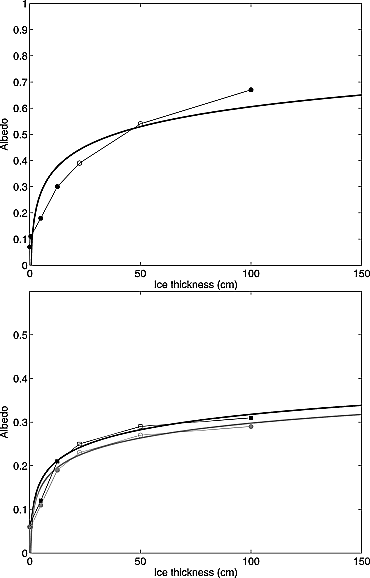
\includegraphics[trim=0cm 0cm 0cm 0cm,clip,width=8cm]{science/jgrd14967-fig-0001.png}
\fi
\]
\caption[Sea ice albedo as a function of ice thickness]{Sea ice albedo as a function of ice thickness for (top)
  visible (VIS, $\lambda < 689\,{\rm nm}$) and (bottom) near--infrared
(NIR, $\lambda > 689\,{\rm nm}$) spectral bands after
\cite{brandt2005}. The filled symbols are measurements, while the open
are interpolated values. The depths are the mean squares fit of the
form $\alpha_{\rm i}=a\log(h_{\rm i})+b$, where $a$ and $b$ are given
in Tab.~\ref{tab_bareseaice}. A distinction is made between direct
(black) and diffuse (gray) irradiance for NIR in
Fig.~\ref{fig_seaicealbedo} (bottom). Reprinted by permission from John
Wiley and Sons. Copyright 2009 by the American Geophysical Union.}\label{fig_seaicealbedo}
\end{figure}

\begin{table}
\caption[Constants for bare sea ice albedo]{Constants for bare sea ice albedo$^\ast$}\label{tab_bareseaice}
\begin{tabular*}{\textwidth}{l@{\extracolsep\fill}llc}\hline
& \multicolumn{1}{c}{$a$} & \multicolumn{1}{c}{$b$} & \multicolumn{1}{c}{Upper threshold} \\\hline
VIS & 0.13 & 0.10 & 0.76 \\
NIR direct & 0.047 & 0.074 & 0.29 \\
NIR diffuse & 0.049 & 0.085 & 0.31 \\\hline
\end{tabular*}
$^\ast$ Bare sea ice albedo is of the form $\alpha_{\rm
  i}=a\log(h_{\rm i}) + b$ proposed from data from \cite{brandt2005}
for visible (VIS, $\lambda < 689 \, {\rm nm}$) and near--infrared
(NIR, $\lambda > 689 \, {\rm nm}$) (direct and diffuse). The upper
threshold values are used for ice thicknesses equal to or above
$1.6\,{\rm m}$ for VIS and $1.0\,{\rm m}$ for NIR.
\end{table}

\subsubsection{Melt ponds}\label{sec_meltpond}

The inclusion of melt ponds in the albedo scheme is very important
from a physical perspective, because of their extensive presence
during summer \cite{perovich2002, tschudi2001, fetterer1998, perovich1997}, and
the large portion of solar energy absorbed by the melt water
(\cite{podgorny1996}). 
Both \cite{schramm1997} and \cite{morassutti1996} provide useful melt pond
albedo parameterizations as a function of pond depth. However, such
schemes cannot be used directly because melt pond depth, and also the
more important melt pond fraction (see
equation~(\ref{eq_seaicealbedo})), is not available in GCMs.

We propose a basic model for melt pond evolution based on the daily
surface ice melt rate from \echam. The temporal evolution of a melt
pond is calculated from the mass balance equation

\begin{equation}\label{eq_massbalance}
\frac{\partial p_{\rm d}}{\partial t} = -\frac{\rho_{\rm i}}{\rho_{\rm
    w}}
\left(\frac{\partial h_{\rm i}}{\partial t}+\frac{\partial p_{\rm
    di}}{\partial t}\right)-\left(\frac{\partial p_{\rm d}}{\partial
  t}\right)_s,
\end{equation}

where $p_{\rm d}$ is the pond depth in m and $\rho_{\rm w}$, $\rho_{\rm
  i}$ are the densities of water and ice, respectively
(Fig.~\ref{fig2}). The first term on the right hand side represents the
melt pond growth through the surface melting of sea ice; the second
term refers to the growth or melting of pond ice $p_{\rm di}$; and the
last term is the constant seepage rate. Pond ice forms if the
temperature of the pond, $T_{\rm w}$, falls below the freezing point,
$T_0$, where $T_{\rm w}$ is calculated from the heat budget equation

\begin{equation}
C_{\rm w}\frac{\partial T_{\rm w}}{\partial t}=H_{\rm sfc}.
\end{equation}

$C_{\rm w}$ is the heat capacity of the pond and $H_{\rm sfc}$ is the
sum of all radiative and turbulent heat fluxes at the surface of the
ice--free pond. For $T_{\rm w} < T_0$, a slab of ice is formed
according to 

\begin{equation}
p_{\rm di} = \left(\frac{C_{\rm w}}{L_{\rm f}\rho_{\rm
      i}}\right)(T_0-T_{\rm w}),
\end{equation}

where $L_{\rm f}$ is the latent heat of fusion. $T_{\rm w}$ is then
reset to $T_0$ and is kept fixed, independent of the sign of $H_{\rm
  sfc}$, because the pond water is forming on top of the ice. The
surface temperature of the ice, $T_{\rm i}$, is calculated from the
heat budget of a thin slab of ice (1~cm) at the surface

\begin{equation}
C_{\rm i}\frac{\partial T_{\rm i}}{\partial t}=H_{\rm sfc}+H_{\rm c},
\end{equation}

where $C_i$ is the heat capacity of the thin upper slab of pond ice
and $H_{\rm c}$ is the conductive heat flux through the ice given by

\begin{equation}\label{eq_condheatflux}
H_{\rm c}=\frac{\kappa_{\rm i}}{p_{\rm di}}(T_0-T_{\rm i})\ge 0,
\end{equation}

where $\kappa_{\rm i}$ is the thermal conductivity of ice.

\begin{figure}[htb]
\[
\ifpdf
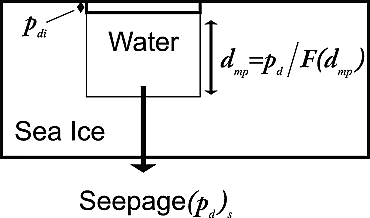
\includegraphics[trim=0cm 0cm 0cm 0cm,clip,width=8cm]{science/jgrd14967-fig-0002.png}
\fi
\]
\caption[A schematic drawing of a melt pond]{A schematic drawing of a melt pond describing a few of the
  variables in
  equations~(\ref{eq_massbalance})--(\ref{eq_condheatflux}). Reprinted by permission from John
Wiley and Sons. Copyright 2009 by the American Geophysical Union.}\label{fig2}
\end{figure}

Melt pond formation will not start before the snow on top of the sea
ice has melted away. If a slab of pond ice $p_{\rm di}\ge 1\,{\rm cm}$
is forming, the melt pond fraction is set to zero. The final closing
of the melt pond in fall is generally caused by vanishing melting and
constant seepage, resulting in $p_{\rm d} \le 0$, or by freezing if
the pond is totally frozen or if a thick ice layer has been formed
($p_{\rm di}=10\,{\rm cm}$). In all these cases the pond is closed,
i.e., $p_{\rm d}$ is set to zero.

To provide an estimate of the melt pond fraction, we propose to
calculate it from the melt pond depth (similar to what is done for
the snow cover fraction in GCMs) using a parameterization of the
results from a number of simulations using a small--scale melt pond
model (\cite{luethje2006}). The model treats the ice surface as a
porous medium. Melt water drains through the ice to the ocean at a
constant rate ($0.8\,{\rm cm/d}$) and the melt water left on the
surface percolates to lower lying areas to form melt ponds. The melt
rate is kept constant during the melt season, but is enhanced where
melt ponds form, to simulate the lower albedo of the melt ponds.
The model discretizes the space and time domain using a finite
differences scheme. For relating the melt pond depth and fraction
covered for different climate scenarios, the model was run with the
same input parameters as described in details by \cite{luethje2006} in
the study of \cite{pedersen2009}. The
melt rate for the ice surface was varied from $1.0\,{\rm cm/d}$ to
$3.0\,{\rm cm/d}$ (in steps of $0.1\,{\rm cm/d}$), while the enhanced
melt rate under the melt ponds was kept at twice the ice surface melt
rate. This was done for both a MYI and a FYI setting, resulting in a
total of 42~model runs, with a melt season of 71~days. The mean daily
fraction of the surface covered by melt ponds is plotted against the
daily mean melt pond depth in Fig.~\ref{fig3} (for FYI and MYI separately).

\begin{figure}[htb]
\[
\ifpdf
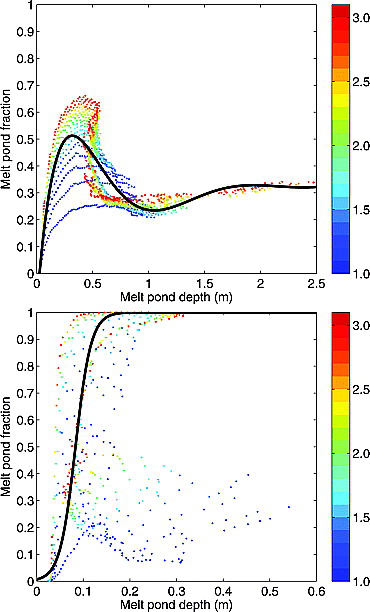
\includegraphics[trim=0cm 0cm 0cm 0cm,clip,width=8cm]{science/jgrd14967-fig-0003.png}
\fi
\]
\caption[Melt pond depth versus meltpond fraction]{Melt pond depth versus meltpond fraction for (top) multiyear
  ice (MYI) and (bottom) first year ice (FYI). The thick lines
  represent the best fit to the data. For MYI the best fit is
  represented by a 8--degree polynomial (equation(\ref{eq_polynom})),
  and for TYI it is represented by a hyperbolic tangent (equation
  (\ref{eq_tanh})). The scatter plot is based on the melt pond model
  by \cite{luethje2006} by using melt rates ranging from $1\,{\rm
    cm/d}$ to $3\,{\rm cm/d}$ (in steps of $0.1\,{\rm cm/d}$) as
  indicated by the color bar. Reprinted by permission from John
Wiley and Sons. Copyright 2009 by the American Geophysical Union.}\label{fig3}
\end{figure}

To connect the melt pond fraction to the melt pond depth for MYI
(Fig.~3, top), an 8--degree polynomial was fitted to the data points:

\begin{equation}\label{eq_polynom}
f_{\rm mp}= a d^8_{\rm mp}+b d^7_{\rm mp}+ c d^6_{\rm mp}+ d d^5_{\rm
  mp}+ e d^4_{\rm mp}+ f d^3_{\rm mp}+ g d^2_{\rm mp}+ h d_{\rm mp}+ i
\end{equation}

where $d_{\rm mp}$ is th melt pond depth in m, and the constants $a$
to $i$ are given in Tab.~\ref{tab_meltpondfit}.
\begin{table}[tb]
\begin{scriptsize}
\caption{Constants for melt pond fraction as a function of melt pond
  depth for multiyear ice}\label{tab_meltpondfit}
\begin{tabular*}{\textwidth}{c@{\extracolsep\fill}cccccccc}\hline
a & b & c & d & e & f & g & h & i\\\hline
-0.00724636 & 0.14438 & -1.19140 & 5.25995 & -13.37101 & 19.53030 &
-15.27019 & 5.26674 & -0.12549 \\\hline
\end{tabular*}
\end{scriptsize}
\end{table}
Fig.~\ref{fig3} (top) shows melt pond depths up to $2.5\,{\rm m}$ for
unrealistically high melt rates ($2.5-3.0\,~{\rm cm/d}$) during the
end of the 71 simulated days. Such depths are not realistic, and were
only included to avoid reaching outside the range of possible melt
pond depth. For FYI, the connection between fraction and depth is more
complex (Fig.~\ref{fig3}, bottom). For small melt rates, the
relationship is similar to that for MYI, but for more realistic melt
rates, the relationship is better described by a hyperbolic tangent
function,

\begin{equation}\label{eq_tanh}
f_{\rm mp}=0.5 \tanh(30 d_{\rm mp} - 2.5) + 0.5.
\end{equation}

Since melt ponds on FYI are mostly important in the beginning and
middle of the melt season, before the ice breaks up, the fit is
created to correspond best with this data, and less with the model
data from later in the melt season.

Regression equations were used for calculating the melt pond albedo
from melt pond depth from observations of melt pond albedo in the
Canadian Arctic Archipelago in spring and summer by~\cite{morassutti1996}:

\begin{equation}
\alpha_{\rm mp}=a+\exp(-b d_{\rm mp}-c)
\end{equation}

where $a$, $b$, and $c$ are regression coefficients, determined for
VIS ($400-689\,{\rm nm}$) and NIR ($689-1000\,{\rm nm}$) bands under
different light conditions (Tab.~\ref{tab_constmelt}). The exponential
albedo decay is large for the first $10-20\,{\rm cm}$ of pond depth,
and for deeper melt ponds the albedo is relatively constant.
An overview of the impact of melt ponds on Arctic sea ice is given in
the model study of \cite{roeckner2012}.
\begin{table}
\caption[Constants for melt pond albedo]{Constants for melt pond albedo$^\ast$}\label{tab_constmelt}
\begin{tabular*}{\textwidth}{l@{\extracolsep\fill}ccc}\hline
 & $a$ & $b$ & $c$ \\\hline
VIS direct & 0.336 & \cw{0}9.457 & 1.061 \\
VIS diffuse & 0.413 & 24.014 & 1.086 \\
NIR direct & 0.017 & 18.904 & 0.909 \\
NIR diffuse & 0.061 & 17.449 & 1.075 \\\hline
\end{tabular*}
$^\ast$Melt pond albedo $\alpha_{\rm mp}$ is of the form $\alpha_{\rm
  mp}=a+\exp(-b d_{\rm mp} - c)$ as a function of melt pond depth
$d_{\rm mp}$ from~\cite{morassutti1996} for visible (VIS) and
near--infrared (NIR) and direct and diffuse radiation.
\end{table}

\include{atmosphere/sea_ice_prescribed}
% Juergen Bader


\chapter{Atmosphere surface coupling}
The documentation for JSBACH is in progress. Most of the JSBACH components can be found in (\cite{raddatz2007}) and under http://www.mpimet.mpg.de/wissenschaft/land-im-erdsystem/globale-vegetationsmodellierung/jsbach-publikationen.html. For further information please contact Christian Reick (christian.reick@zmaw.de).

\include{atmosphere/lake_model}
\include{atmosphere/albedo}

%\section{Over land}

%\section{Over sea water}

%\subsection{If coupled to MPIOM}

%\subsection{If prescribed}

%\section{Over sea ice}

%\subsection{If coupled to MPIOM}

%\subsection{If prescribed}

\chapter{Model resolutions and resolution dependent parameters}
%++ T. Mauritsen
%\documentclass[10pt,letterpaper,twoside]{article}
%\usepackage{times,amsmath,graphicx,longtable,multicol,natbib}
%\begin{document}

\section{Model resolutions and resolution-dependent parameters\label{sec:paraX}}\label{cXX}

ECHAM 6.0 contains several poorly constrained parameters relating to orographic and non-orographic gravity wave drag, clouds, convection and horizontal diffusion adjusted, or tuned, to yield an acceptable climate and a sufficiently stable model execution. Some of these parameters are adjusted individually for each horizontal and/or vertical discretization of the model. The ECHAM 6.0 model was rigorously tested to run coupled to the MPIOM ocean model in two resolutions, and in atmosphere-only mode in one higher resolution. Additionally, the model can be run in a set of lower and one higher resolutions for testing purposes.


\subsection{Available model resolutions}

For coupled simulations T63L47 was used with the MPIOM GR15 (1.5 degree) ocean resolution in MPI-ESM-LR. T63L95 was used with a higher resolved MPIOM TP04 ocean grid (0.4 degree) in MPI-ESM-MR. For both these setups, spun-up ocean initial states exist from the control simulations submitted to the CMIP5 archive. The model was also tested in atmosphere-only mode with satisfactory results at T127L95. The former model is designated MPI-ESM-HR in the CMIP5 archive. Correspondingly spun-up ocean initial state is not available for these resolution. See table for an overview:

\begin{table}[h]
\begin{center}
\begin{tabular}{l|l|l|l}
\hline\noalign{\smallskip}
ECHAM 6.0 & MPIOM &  Status, tested for: & CMIP5 designator  \\
\noalign{\smallskip}\hline\noalign{\smallskip}
T63L47 & GR15 & Coupled and Uncoupled & MPI-ESM-LR \\
T63L95 & TP04 & Coupled and Uncoupled & MPI-ESM-MR \\
T127L95 & N/A & Atmosphere-only & MPI-ESM-HR \\
\noalign{\smallskip}\hline
\end{tabular}
\end{center}
\end{table}

%It is further possible to run the model in different resolutions, T31L19, T31L31, T31L39, T42L19 and T255L199 for testing purposes. These resolutions have not undergone rigorous testing and it is not %recommended to use them for scientific purposes. We shall therefore not deal with these below.

\subsection{Resolution-dependent parameters}

The parameters that are resolution dependent for maintaining the radiation balance and, thereby, the global mean temperature for the supported resolutions are Cloud mass-flux above the level of non-buoyancy (CMFCTOP), and the Conversion rate from cloud water to rain in convective clouds (CPRCON). See \cite{tiedtke89} for details. The parameter settings are given in the table.

The extra-tropical northern hemisphere tropospheric winds are tuned using orographic wave drag. This is done adjusting the orographic gravity wave drag strength, GKDRAG and GKWAKE, which we tend to set equal. The largest sub-grid scale orographic peaks must exceed the mean topography by GPICMEA, while the sub-grid scale orography standard deviation must exceed GSTD, before the scheme is activated. For details see \cite{lott99}. Resolution-dependent parameters are given in the table.

Non-orographic wave drag is modeled using a fixed background wave source field. The strength a meridional shape of the source field is adjusted to yield a good representation of the stratospheric circulation and variability, in particular the quasi-biennial oscillation. If LRMSCON\_LAT is set to .true. the source field is latitude-dependent. At latitudes equator-ward of +/- LAT\_RMSCON\_LO = 5 degrees the source strength is RMSCON\_LO, and at latitudes poleward of +/- LAT\_RMSCON\_HI = 10 degrees the strength is set to RMSCON\_HI, which is 1.0 for all resolutions. Between these latitudes the strength is interpolated. The parameters may be controlled at runtime through the 'gwsctl' namelist, and their default values for the supported resolutions are given in the Table:
\begin{table}[h]
\begin{center}
\begin{tabular}{l|l|ccc}
\hline\noalign{\smallskip}
Parameter & Subroutine & T63L47 & T63L95 & T127L95\\
\noalign{\smallskip}\hline\noalign{\smallskip}
CMFCTOP & mo\_cumulus\_flux & 0.21 & 0.23 & 0.205 \\
CPRCON & mo\_cumulus\_flux & $2.0\cdot10^{-4}$ & $2.0\cdot10^{-4}$ & $1.3\cdot10^{-4}$ \\
GKDRAG & mo\_ssodrag & 0.50 & 0.25 & 0.50  \\
GKWAKE & mo\_ssodrag & 0.50 & 0.25 & 0.50  \\
GPICMEA & mo\_ssodrag & 400 m & 400 m & 200 m \\
GSTD & mo\_ssodrag & 100 m & 100 m & 50 m  \\
RMSCON\_LO & setgws & 1.2 & 1.2 & 1.05  \\
%RMSCON\_HI & setgws & 1.0 & 1.0 & 1.0 &  1.0 \\
\noalign{\smallskip}\hline
\end{tabular}
\end{center}
\end{table}




\subsection{Code implementation}\label{sec.codeimplementation}

The resolution-dependent parameters are hard-coded into several subroutines. Thereby, the model configures itself when it is executed at a certain resolution. That also means that it requires code-modifications to run the model in a different resolution than those that are implemented. Some of the affected subroutines are listed in the Table. Each subroutine contains a series of IF- or CASE-statements that configures the model according to horizontal and/or vertical resolution. If a resolution is not supported by the code, execution will typically finish with an error message: 'Truncation not supported'.

In addition to the parameters treated here for the supported resolutions, a number of parameters vary among the unsupported resolutions, and the settings of these have not been evaluated. These pertain to snow and ice albedos (mo\_surface\_ice.f90), cloud optical properties (mo\_newcld\_optics.f90) and cloud microphysics (mo\_cloud.f90). Horizontal diffusion and sponge-layer parameters are also set for each resolution in mo\_hdiff.f90 and in setdyn.f90, while the time-step length needs to be set in mo\_time\_control.f90. See chapter \ref{sec:dyncore} for details.




% T. Mauritsen

\chapter{External data}

%++S.Rast
\section{Solar irradiation\label{sec:externaldata_solar}}

The total solar irradiance $\Psi$ of the earth is defined as the incoming
solar energy at the top of the atmosphere per area, normed to a
sun--earth distance of 1~astronomical unit, and integrated over the
whole range of wavelengths $\left[0,\infty\left[\right.\right.$
(units: W/m$^2$).
The solar irradiance $\lambda\mapsto\psi(\lambda)$ is the incoming
solar energy at the top of the 
atmosphere per area and wavelength of electromagnetic radiation, also
normed to a sun--earth distance of 1~astronomical unit (units: W/m$^2$/nm). 
Solar irradiance $\psi$ and therefore $\Psi$ vary with time. The
variation patterns depend on 
the wave length and are therefore different for the various spectral
bands of \echam. For the old 6--band radiation scheme of ECHAM5, only the total
solar irradiance $\Psi$ was prescribed and the distribution onto the spectral
bands was fixed. This means that for a spectral band
$[\lambda_1,\lambda_2]$, the incoming energy
\begin{displaymath}
\psi_{\lambda_1,\lambda_2}:=\int\limits_{\lambda_1}^{\lambda_2}\psi(\lambda)\,d\lambda 
\end{displaymath} 
was determined from fixed fractions
$\xi_{\lambda_1,\lambda_2}:=\psi_{\lambda_1,\lambda_2}/\Psi$. For the
new 14--band SRTM 
radiation scheme implemented in \echam{} (section~\ref{sec_shortwave}),
the incoming solar irradiance of each band 
$\psi_{\lambda_1,\lambda_2}$ can vary independently with time.



\subsection{Historic}

\begin{sloppy}
For historic and future solar irradiance data we follow as closely as
possible the recommendations 
for CMIP5 as provided by the SPARC/SOLARIS project as  given on the
web site ({\tt
  http://www.geo.fu-berlin.de/en/met/ag/strat/forschung/SOLARIS/Input\_data/}
\\ 
{\tt CMIP5\_solar\_irradiance.html}).
Historic data for the period 1850 until 2008 was reconstructed based
on observations and proxy data by J. Lean (Naval Research Laboratory,
Washington D.C., USA). Detailed information on the reconstruction is
provided at the above mentioned web site.  
Total solar irradiance variations were reconstructed as described by
\citet{froehlich_04} based on time series of sunspots and faculae. 
The spectral dependence of the solar irradiance and its variability
was determined from the 
spectral dependence of the sunspot blocking and 
facular brightening, as described in detail by \citet{lean_00}. 
Data are provided for wavelengths from 100 to 100000 nm with a
spectral resolution of 1 nm for small  
wavelengths and increasing with wavelength. For use in \echam{} the
original data have been averaged over the wavelength bins of  
the SRTM code as given in table~\ref{tab_srtm} and scaled in order to
provide the full TSI in the wavlength range covered by the SRTM
scheme. 
Additionally, as recommended by SPARC/SOLARIS, the orginal data have
been multiplied by 
a factor of 0.9965. This was done in order to obtain a TSI close 
to 1361 W/m$^2$ as suggested by recent observations instead of about
1368 W/m$^2$ assumed earlier. 
The temporal resolution of the original data is annually until 1881
and monthly starting in 1882. 
For use in \echam{} we have linearly interpolated the annual data
available before 1882 to monthly values in order to 
provide consistent data sets over the full historic period. However,
it should be kept in mind that short period variability of solar
irradiance 
used as input in the CMIP5 simulations is larger after than before
1882 (see Fig.~\ref{fig:eps}). 
\end{sloppy}

\subsection{Scenarios}
For the future scenarios it is recommended to repeat solar cycle 23, i.e. irradiance data of the period 
May 1996 to July 2008 for August 2008 to Oct 2020, Nov 2020 to Jan 2033, etc. 
This means that data files for the 49 years from 2008 to 2056 can be used as input for the years 2057 to 2105 and 
further repeated for later periods. The time series of monthly TSI integrated from the spectral irradiances used for
the period 1850--2100 is presented in Fig.~\ref{fig:eps}.


Monthly averaged spectral irradiance data for the years 1850--2100 are stored in yearly files
{\tt swflux\_14band\_yyyy.nc}, {\tt yyyy} being the year.
These files contain the monthly mean values of $\Psi$ as {\tt TSI} and
$\psi_{\lambda_1,\lambda_2}$ as {\tt SSI} in W/m$^2$. These variables
are read into \echam{} and linearly interpolated with respect to time to
the actual model radiation time step.






\begin{figure}[htb]
\[
\ifpdf
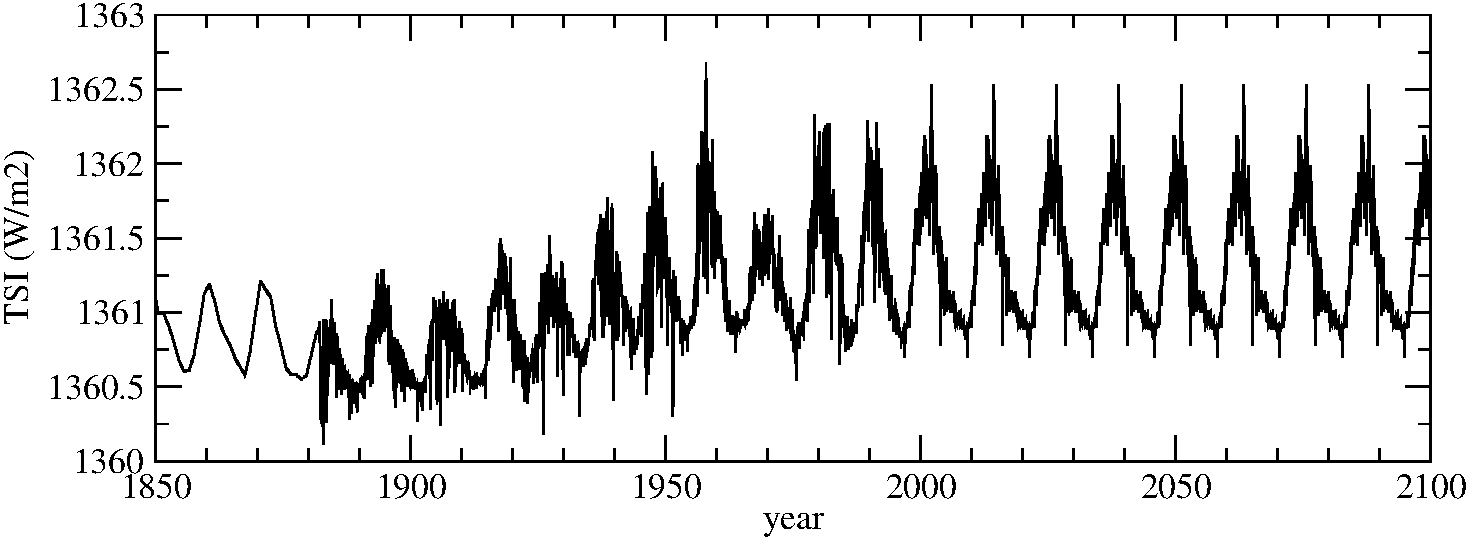
\includegraphics[width=15cm]{externaldata/tsi_1850-2100.pdf}
\else
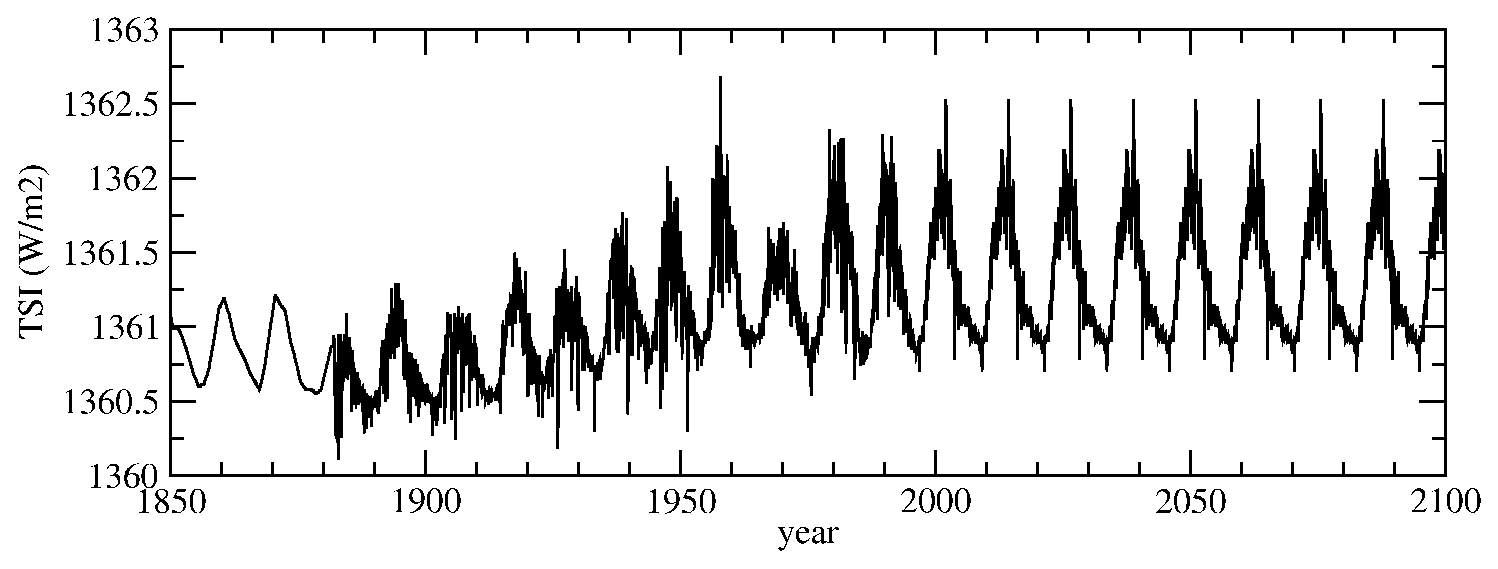
\includegraphics[width=15cm]{externaldata/tsi_1850-2100.eps}
\fi
\]
\caption{\label{fig:eps}Monthly averaged total solar irradiance (TSI) resulting from the spectrally resolved irradiance used in CMIP5
simulations with \echam.}
\end{figure}

\subsection{Climatologies}

Several choices of climatological solar irradiance (i.e.~constant solar
irradiance that is independent of time) are available: The
original ``SRTM'' values, a solar irradiance averaged over the years
1844--1856 (``preindustrial'') 
that was used in the preindutrial control simulations of CMIP5, 
and a solar irradiance averaged over the years 1979--1988 (``amip'').
In the latter two cases averaging was performed over data from the
time dependent historic data set as described below. 
For simulations with constant solar irradiance it is recommended to
use the ``preindustrial'' or ``amip'' 
climatological values which provide total solar irradiances (TSI) of
close to 1361 W/m$^{2}$ to which \echam{} has been tuned. 
The original TSI of ``SRTM'' is of about 1368 W/m$^{2}$ (see
table~\ref{tab_srtm}). 
All the mentioned climatologies do not have to be read in from
external files but can be accessed by specific choices 
of namelist parameters.


\begin{table}[hb]
\caption{$\psi_{\lambda_1,\lambda_2}$ in $\rm W/m^2$ as defined for the original
SRTM radiation scheme (SRTM), for the preindustrial period (preind),
and the amip period (amip). The resulting total solar irradiance
(solar 
constant) $\Psi$ is $1368.222\,{\rm W/m^2}$ for the original SRTM
scheme, $1360.875\,{\rm W/s^2}$ for the preindustrial period, and
$1361.371\,{\rm W/m^2}$ for the amip period.}\label{tab_srtm} 
\begin{tabular*}{\textwidth}{c@{\extracolsep\fill}cccc}\hline\hline
band/nm & 3077 --\cw{0}3846&2500 --\cw{0}3077&2151 --\cw{0}2500&1942 --\cw{0}2151\\
index & 1 & 2 & 3 & 4 \\
$\psi_{\lambda_1,\lambda_2}$ (SRTM) 
& \cw{0}12.1096\cw{0} & \cw{0}20.3651\cw{0} & \cw{0}23.7297\cw{0} &\cw{0}22.4277\cw{0}\\
$\psi_{\lambda_1,\lambda_2}$ (preind) 
& \cw{0}11.9500\cw{0} & \cw{0}20.1461\cw{0} & \cw{0}23.4030\cw{0} &\cw{0}22.0944\cw{0}\\
$\psi_{\lambda_1,\lambda_2}$ (amip) 
& \cw{0}11.9505\cw{0} & \cw{0}20.1477\cw{0} & \cw{0}23.4039\cw{0} &\cw{0}22.0946\cw{0}\\\hline
band/nm & 1626 --\cw{0}1942&1299 --\cw{0}1626&1242 --\cw{0}1299&\cw{0}788 --\cw{0}1242\\
index & 5 & 6 & 7 & 8 \\
$\psi_{\lambda_1,\lambda_2}$ (SRTM) 
& \cw{0}55.6266\cw{0} & 102.932\cw{00} & \cw{0}24.2936\cw{0} &345.742\cw{00}\\
$\psi_{\lambda_1,\lambda_2}$ (preind) 
& \cw{0}55.4168\cw{0} & 102.512\cw{00} & \cw{0}24.6954\cw{0} &347.472\cw{00}\\
$\psi_{\lambda_1,\lambda_2}$ (amip) 
& \cw{0}55.4140\cw{0} & 102.513\cw{00} & \cw{0}24.6981\cw{0} &347.536\cw{00}\\\hline
band/nm&\cw{0}625 --\cw{00}788&\cw{0}442 --\cw{00}625&\cw{0}345 --\cw{00}442&\cw{0}263 --\cw{00}345\\
index & 9 & 10 & 11 & 12 \\
$\psi_{\lambda_1,\lambda_2}$ (SRTM) 
& 218.187\cw{00} & 347.192\cw{00} & 129.495\cw{00} &\cw{0}50.1522\cw{0}\\
$\psi_{\lambda_1,\lambda_2}$ (preind) 
& 217.222\cw{00} & 343.282\cw{00} & 129.300\cw{00} &\cw{0}47.0762\cw{0}\\
$\psi_{\lambda_1,\lambda_2}$ (amip) 
& 217.292\cw{00} & 343.422\cw{00} & 129.403\cw{00} &\cw{0}47.1426\cw{0}\\\hline
band/nm & \cw{0}200 --\cw{00}263&3846 --12195&&\\
index & 13 & 14 &  &  \\
$\psi_{\lambda_1,\lambda_2}$ (SRTM) 
& \cw{00}3.07994 & \cw{0}12.8894\cw{0} & &\\
$\psi_{\lambda_1,\lambda_2}$ (preind) 
& \cw{00}3.17212 & \cw{0}13.1807\cw{0} & &\\
$\psi_{\lambda_1,\lambda_2}$ (amip) 
& \cw{00}3.17213 & \cw{0}13.1808\cw{0} & &\\\hline\hline
\end{tabular*}
\end{table}

%--S.Rast
%\section{CO2, CH4, N2O, CFCs}

%++M.Esch
\section{CO2, CH4, N2O, CFCs}

\subsection{1850-present, present to 2100 and beyond}

The data sets for pre-industrial, historical and future concentrations 
of well mixed greenhouse gases have been provided by IIASA as
global mean time series at:
\newline
{\tt http://www.iiasa.ac.at/web-apps/tnt/RcpDb/}

For historical times and the future until 2100 the Representative Concentration Pathway (RCP)
scenarios are used. RCP 4.5 is a stabilization scenario where total radiative forcing is stabilized before 2100
\cite[]{thomson2011}.
RCP 8.5 is characterized by increasing greenhouse gas emissions over time \cite[]{riahi2011}.
RCP 2.6, also known as RCP 3-PD, first 
peaks at 3.1 Wm$^{-2}$ around mid-century, and then declines to 2.6 Wm$^{-2}$ by 2100 \cite[]{vanVuuren2011}.

For the years 2100 to 2300 the proper RCP scenarios have been extended,
for the purpose of climate modelling \cite[]{meinshausen2011}.

Further information on the original data can be found on the given IIASA website.

Starting from the original data in ASCII-Format the greenhouse gases relevant for \echam{} \newline
(CO2, CH4, N2O, CFC-11 and CFC-12) were extracted and simply rewritten in netcdf-Format.
Units are ppmv for CO2, ppbv for CH4 and N2O, and pptv for CFC-11 and CFC-12.

%--M.Esch

%\subsection{Historic}
%\subsection{Scenarios}

%++S.Rast
\section{Ozone}

Ozone absorbs in the solar wave length spectrum but also in the
thermal wave length spectrum thus acting as a greenhouse
gas. According to \citet[p.528]{brasseur1999} 
it contributes about 16\% to the total radiative forcing due to
increases in greenhouse 
gas concentrations for the period from 1900 to 1990.
The mass mixing ratio of ozone in the
atmosphere strongly varies with altitude and geographical
latitude. The variation with geographical longitude at fixed latitude
and altitude are less pronounced but not negligible. Therefore, it is
preferable to use 3--dimensional ozone data. The ozone concentration
also depends on time, but climatological data may be useful for
non--transient simulations.
 
\subsection{Historic}

The data set for historic ozone concentrations was created within the projects
AC\&C and SPARC for simulations (e.g.~CMIP5)
that do not take interactive chemistry into account
(\cite{cio117}). The ozone data 
are prepared using
satellite (SAGE~I and~II) and radiosonde data for the stratosphere
and model data (CAM3.5 and NASA-GISS PUCCINI) for the troposphere.
These historic ozone data include the ozone reduction in the
stratosphere caused by ozone depleting species.
A short description of the construction is given on:
\newline
{\tt http://www.pa.op.dlr.de/CCMVal/AC\&CSPARC\_O3Database\_CMIP5.html.}\newline

Ozone data are provided in terms of 3--dimensional monthly
averages. However, in the stratosphere 
the data set does not vary with longitude, so that only in the troposphere
real 3D information is available.

Original data exist only for altitudes with
pressures larger than 1~hPa. Since the standard vertical resolutions
include model layers with pressures as low as 0.01~hPa, 
the dataset was extended upward by
Chris Bell (University of Reading) applying the following
formula:\\
\begin{equation}
O_3(z) = O_3(1~\textrm{hPa}) * \exp(-(z-z(1~\textrm{hPa}))/H),
\end{equation}
with $H$ set to 7 km and $O_3(z)$ denoting the ozone concentration at altitude $z$. 

The resulting 3--dimensional ozone data for the years 1850--2008 are given as
monthly mean values on 39~pressure levels which are listed in
Table~\ref{tabpres}. The data are organized in yearly files {\tt
  T\{RES\}\_ozone\_CMIP5\_{\it yyyy}.nc} where {\tt \{RES\}}
represents the horizontal resolution and {\tt\it yyyy} the
respective year between 1850 and~2008. These files contain the
pressure levels in the variable {\tt plev} and the ozone volume mixing
ratio in the variable {\tt O3}. Height interpolation is performed by \echam. 

\begin{table}[hb]
\caption{Pressure levels in~Pa of ozone climatology}\label{tabpres}
\begin{tabular*}{\textwidth}{c@{\extracolsep\fill}ccccccc}\hline
\cw{00000}1& \cw{00000}3& \cw{00000}5& \cw{0000}10& \cw{0000}20&
\cw{0000}30& \cw{0000}50& \cw{000}100 \\
\cw{000}150& \cw{000}200& \cw{000}300& \cw{000}500& \cw{000}700&
\cw{00}1000& \cw{00}1500& \cw{00}2000 \\ 
\cw{00}3000& \cw{00}5000& \cw{00}7000& \cw{00}8000& \cw{0}10000&
\cw{0}15000& \cw{0}20000& \cw{0}25000 \\ 
\cw{0}30000& \cw{0}40000& \cw{0}50000& \cw{0}60000& \cw{0}70000&
\cw{0}85000& 100000 & \\\hline 
\end{tabular*}
\end{table}

\subsection{Scenarios}
Future ozone scenarios for the period 2008--2099 are provided from the
same source mentioned in the case of historic data. 
In the case of the future the data set is based on multi--model
projections provided in the  
framewok of the SPARC Chemistry-Climate Model Validation Activity
(CCMVAL, see \cite{cio117,eyr103}).
As in the case of historical ozone the original dataset also did only
extend up to 1 hPa 
and was extended upward by Chris Bell. This dataset however does not
include a solar cycle. 
For CMIP5 simulations with \echam
solar cycle 23 is repeated for the future, i.e. the solar variability for
the period May 1996 to July 2008 is repeated for August 2008 to
October 2020, November 2020 to January 2033, etc. (see
section~\ref{sec:externaldata_solar}). 
In order to obtain future ozone concentrations consistent with the
assumptions for solar irradiance 
a multi-linear regression analysis was performed for the historical
ozone data using  the solar irradiance 
at a wavelength of 180.5 nm and the EESC (Equivalent Effective Stratospheric Chlorine) content as regressors.
The resulting regression coefficients for the ozone dependence on solar irradiance and the assumed future irradiance at 180.5 nm 
were then used to add a solar cycle dependence to the future
stratospheric ozone. Tropospheric data (for $p \ge 100$ hPa) have not
been 
modified as the solar cycle dependence calculated from the historic
data for this altitude regime is negligible.  

AC\&C/SPARC ozone projections are available only until 2099. For the
years starting with 2100 the 
original ozone data for the year 2099 are used, but modulated by a
solar cycle effect as described above for the years 
until 2099. Data files were prepared until the year 2399.

The total column ozone for various geographical regions for the
years 1850 to 2099 is presented in Fig.~\ref{fig:ozone}.

\begin{figure}[htb]
\[
\ifpdf
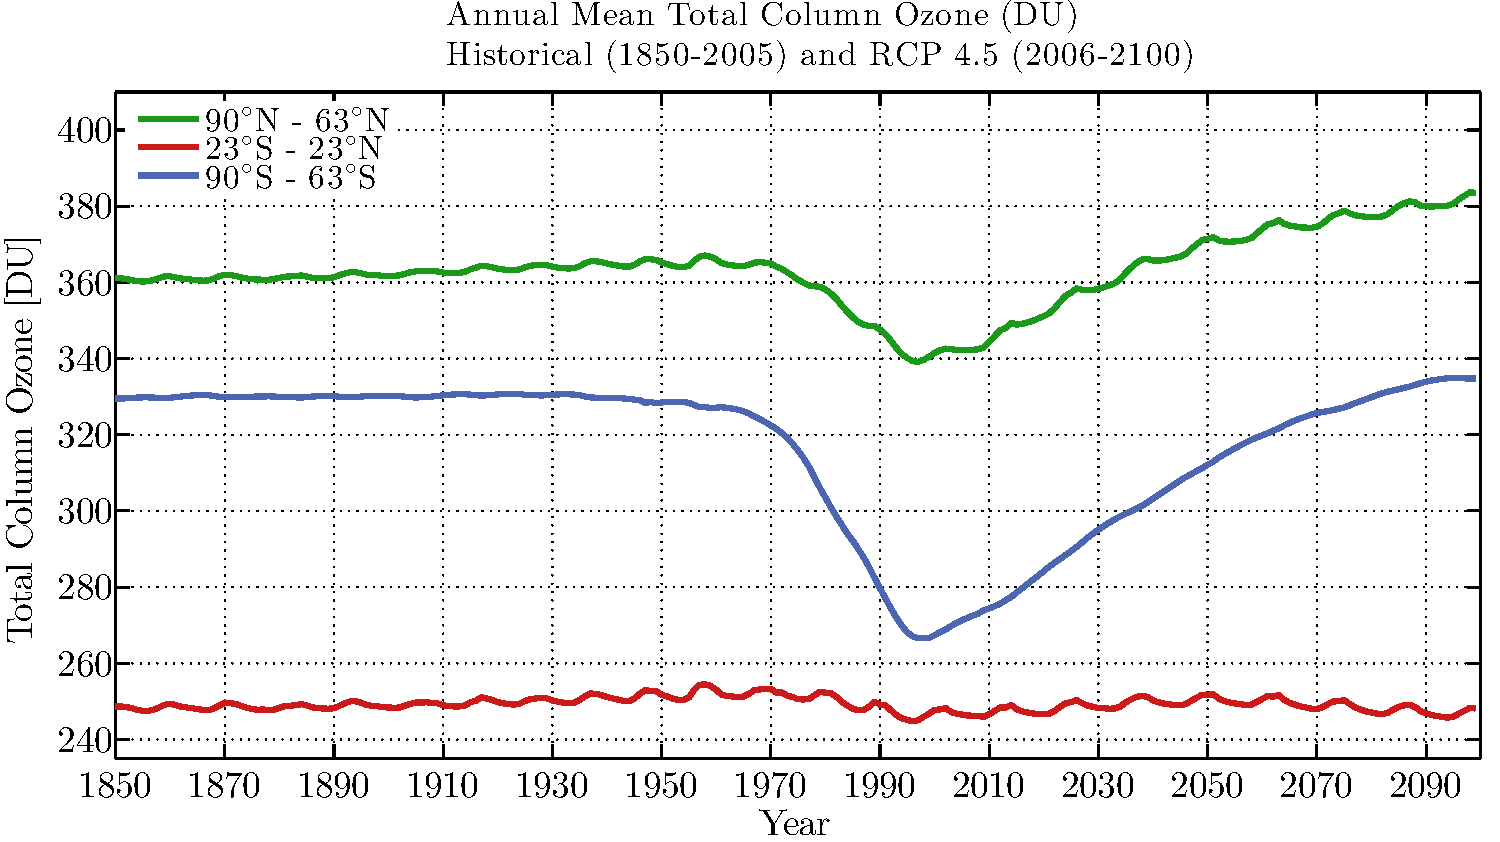
\includegraphics[width=12cm]{externaldata/total_column_ozone_annual.pdf}
\else
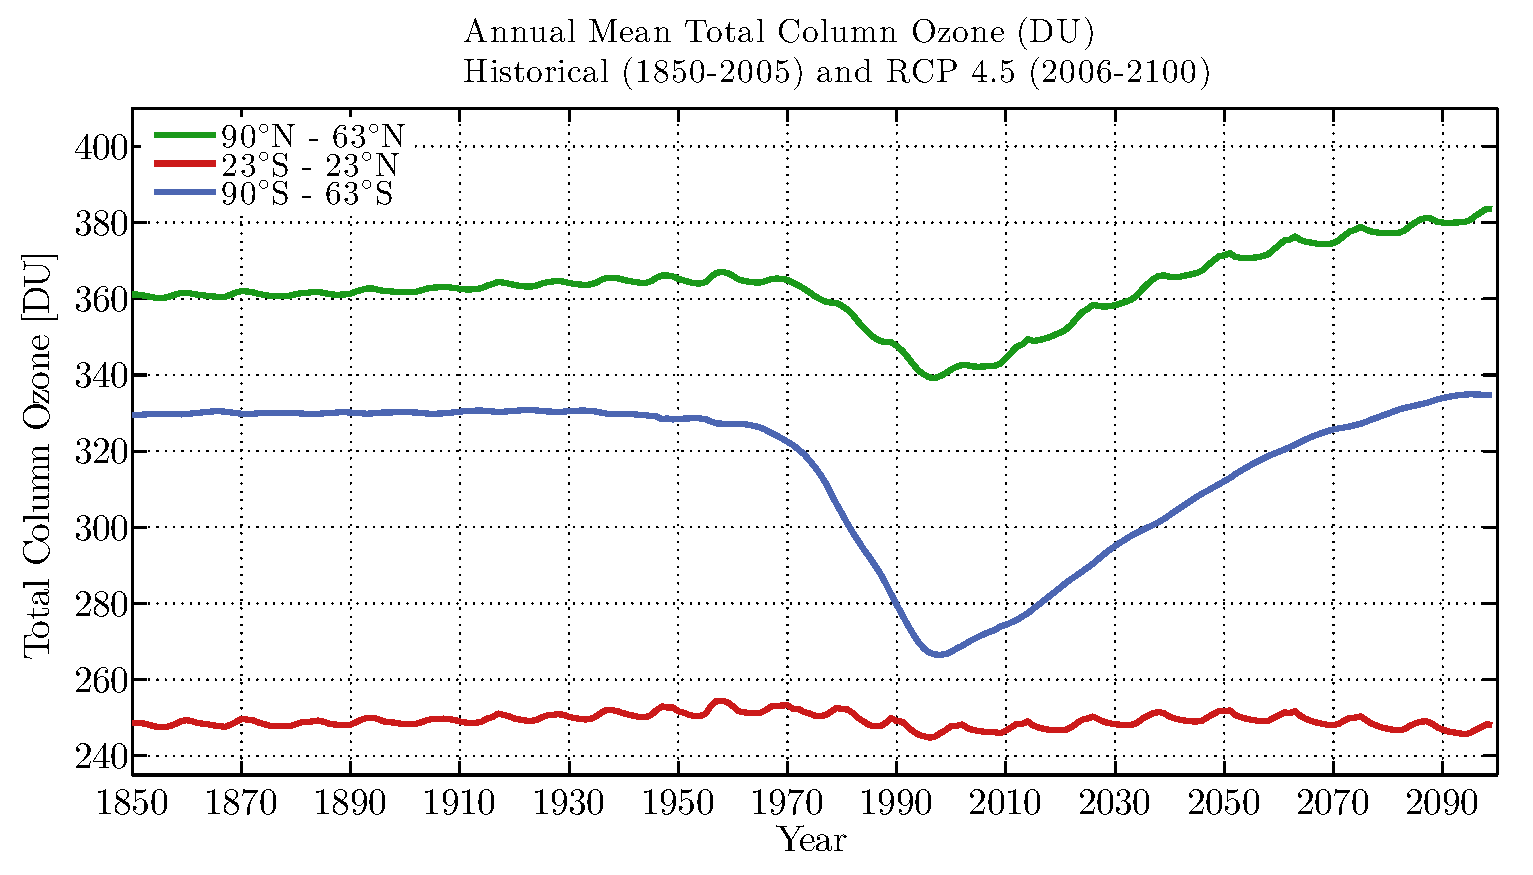
\includegraphics[width=12cm]{externaldata/total_column_ozone_annual.eps}
\fi
\]
\caption{Annual total column ozone for various geographical regions
  for the years 1850 to 2099. Figure courtesy by Alexander Haumann}\label{fig:ozone}
\end{figure}


As in the case of historical data, 3--dimensional ozone data for the
years 2009--2399 are given as 
monthly mean values on 39~pressure levels.
The data are organized in yearly files 
{\tt T\{RES\}\_ozone\_CMIP5\_\{rcp\}\_{\it yyyy}.nc} where {\tt \{RES\}}
represents the horizontal resolution and {\tt\it yyyy} the
respective year. \{rcp\} can have the values RCP26, RCP45 or RCP85,
and indicates the respective representative concentration pathway   
(i.e. future greenhouse gas scenario) for which the data set is valid. 
While in the stratosphere (for $p < 100$ hPa) all data sets are equal,
the AC\&C/SPARC projections differ for tropospheric ozone. 





\subsection{Climatologies}

In some cases, mean values of historic ozone concentration over time
may be used as climatological boundary condition. Therefore, monthly
mean ozone 
concentrations over eleven years for the years 1850--1860 ({\tt
  T\{RES\}\_ozone\_CMIP5\_1850-1860.nc} to be used for preindustrial simulations
  and the years 1979-1988 ({\tt
  T\{RES\}\_ozone\_CMIP5\_1979-1988.nc}) are also provided. In both cases the averaging
was performed over about one full solar cycle in order to avoid potential
biasing from biased solar irradiance.


\section{Aerosols}

Aerosols affect the distribution of radiative energy in the atmosphere
by scattering and absorption of electromagnetic radiation. This is the
direct aerosol effect. Aerosols also modify cloud optical properties
and influence the cloud formation processes and precipitation. Since
this also acts on radiation, but the aerosol particles are involved by
the intermediate of clouds, this is called the indirect aerosol
effect. The radiative transfer calculation of
\echam{} needs time dependent 3--d fields of (1) the extinction $\zeta$
by aerosols, (2) the single scattering albedo $\omega$ (SSA), and (3) the
asymmetry factor $g$ for a detailed consideration of the direct
aerosol effect. These quantities depend on the wavelength of the
electromagnetic radiation and have to be provided for each of the
14~solar radiation bands and the 16~thermal radiation bands used in
\echam. In the thermal radiation range, the knowledge of $\zeta$ and
$\omega$ is
sufficient, since the radiative transfer calculation does not account
for scattering in this wavelength regime.


\subsection{Tropospheric aerosols}\label{sec.tropaerosols}

In this section, we describe the generation of a data set of optical
properties of tropospheric aerosols for the historic period of
1850 to 2000
and for three different future 
emission scenarios (\cite{mos107}) until 2100. 
Tropospheric aerosol is partly anthropogenic and highly diverse in
concentration, size, 
and composition.

We combine complete and consistent background
maps of monthly mean aerosol optical properties from global model
results with high 
quality monthly averages from ground based remote sensing. All
equations are valid for monthly means. We
distinguish between 
fine mode aerosols with 
particle radii smaller than $\rm 0.5\,\mu m$ and coarse mode aerosols
with radii equal or larger than $\rm 0.5\,\mu m$. Coarse mode aerosols
are assumed to be of natural origin comprising dust and sea salt. Fine
mode aerosols consist of sulfate and organic matter including black
carbon.
The general procedure consists of 7~steps: (1) Establishing 2--d maps
of column properties of the aerosol optical depth (AOD), single
scattering albedo, and the 
{\AA}ngstr\"om parameter at 550~nm for the year~2000, (2)~separating the
AOD into one due to fine and one due to coarse mode aerosols for the year~2000,
(3)~defining the microphysical properties of the coarse mode,
(4)~spreading the 
optical properties to all wavelengths, (5)~defining altitude
profiles, (6)~establishing an anthropogenic (fine mode) AOD for the
year~2000, (7)~extending the anthropogenic AOD
back to the year 1850 and forward to the year~2100 using
selected future emission scenarios. 

\subsubsection{(1) 2--d maps
of column aerosol optical properties for the year~2000}

In a first step, monthly mean values of the total aerosol optical
depth $\tau$ of each column together with one value of the single
scatter albedo $\omega$, and {\AA}ngstr\"om parameter $\alpha$ for
that column were 
determined for light of a wavelength of $\rm 550\,nm$. The background
data are based on maps of medians
of an ensemble of up to
15~different global models all applying a complex aerosol module.
All models simulated the respective quantities for present
day conditions in the frame work of the AeroCom project
(\cite{kin065}). The resulting maps were blended by the use of AERONET 
ground based sun--/sky--photometer data (\cite{hol981}): We first
associated a ``factor of influence'' around each AERONET site being
equal to one at the exact location of the site and tending to zero
with increasing distance from the site. The rate of decrease depends
on how well the measurements of this site repesent the aerosol optical
properties of its
surroundings. The original medians were then multiplied by the factor
of influence times the ratio of the AERONET measurement value and the
original median. Thus, we obtain a map of $\tau$, $\omega$, $\alpha$
with AERONET--similar values near the AERONET sites and median values of the
model ensemble at remote places. 
The above method provides the monthly mean optical properties on a
$1^\circ\times1^\circ$ longitude--latitude grid for all
aerosols. 

\subsubsection{(2) Splitting the
AOD into fine and coarse mode contributions for the year~2000}

In order to split the aerosol optical depth into a part for
fine and coarse mode, we use the {\AA}ngstr\"om parameter. It is
assumed that the {\AA}ngstr\"om parameter is zero for the coarse mode
and that it varies between 1.6 and 2.2 for the fine mode depending on
humidity. Details of this procedure are described by~\cite{kinxxx}.

\subsubsection{(3) Definition of the coarse mode microphysical properties}

In order to derive the coarse mode aerosol optical properties 
at 550~nm, the respective composition and particle size has to be known.
It is assumed that the coarse mode aerosols are ten times less absorbing than
the fine mode aerosols. The initial guess of the coarse mode single
scattering albedo $\omega_{\rm c,0}$ depends on the total aerosol
single scattering albedo $\omega$ and the ratio of the aerosol optical
depth of the fine mode $\tau_{\rm f}$ and the total aerosol optical
depth $\tau$:

\begin{displaymath}
\omega_{\rm c,0}=1-\frac{1-\omega}{1+9\frac{\tau_{\rm f}}{\tau}}
\end{displaymath}

This choice determines the mixing ratio of dust and sea salt aerosols
in the coarse mode. For latitudes between 35$^\circ$~S and
45$^\circ$~N, the fraction of dust was assumed to increase with coarse mode
aerosol optical depth.
In the initial guess, it is assumed that
dust particles have an effective radius of $1.5\,\mu m$
and sea salt particles have an effective radius of
$2.5\,\mu m$. 
However, the size of the dust particles can be set to larger values
in order to avoid unrealistic small values for the single scattering
albedo of the fine mode aerosols. In such cases, the single scattering
albedo of the fine mode is kept at values given by: 

\begin{equation}\label{eqssalimit}
\omega_{\rm f,0}=1-\left(\frac{1}{10}{\rm
  e}^{-3\tau}+\frac{1}{4}\frac{\tau_{\rm f}}{\tau}\right).
\end{equation}

\begin{table}[hp]
\caption{Wavelengths of the 14~bands in the short wavelength range and
  the 16~bands in the long wavelength range as they are used in the
  radiation calculation of \echam{} and the refractive
  indices of sulfate, dust (\cite{sok983}), and sea salt
  (\cite{nil797})}\label{tabwavelengths}  
\begin{tabular*}{\textwidth}{c@{\extracolsep\fill}ccc}\hline
$\lambda_{\rm v}/{\rm nm}$ & sulfate & dust & sea salt \\\hline
\multicolumn{4}{c}{solar radiation}\\\hline
\cw{00}200 --   \cw{000}263 &$1.450+i1.0\times10^{-9}$&$1.450+i0.025$
&$1.510+i1\times10^{-5}$\\
\cw{00}263 --   \cw{000}345 &$1.450+i1.0\times10^{-9}$&$1.450+i0.020$
&$1.510+i1\times10^{-6}$\\
\cw{00}345 --   \cw{000}442 &$1.445+i1.0\times10^{-9}$&$1.450+i0.0025$
&$1.500+i2\times10^{-8}$\\
\cw{00}442 --   \cw{000}625 &$1.432+i1.0\times10^{-9}$&$1.450+i0.001$
&$1.490+i1\times10^{-8}$\\
\cw{00}625 --   \cw{000}778&$1.427+i5.2\times10^{-8}$&$1.450+i0.00095$
&$1.480+i1\times10^{-7}$\\
\cw{00}778 --  \cw{00}1242&$1.422+i1.3\times10^{-6}$&$1.450+i0.00075$
&$1.470+i1\times10^{-4}$\\
\cw{0}1242 --  \cw{00}1299&$1.413+i7.9\times10^{-6}$&$1.450+i0.00060$
&$1.470+i3.3\times10^{-4}$\\
\cw{0}1299 --  \cw{00}1626&$1.406+i9.0\times10^{-5}$&$1.450+i0.00080$
&$1.460+i5.5\times10^{-4}$\\
\cw{0}1626 --  \cw{00}1942  &$1.393+i5.1\times10^{-4}$&$1.450+i0.0010$
&$1.450+i1\times10^{-3}$\\
\cw{0}1942 --  \cw{00}2151  &$1.382+i1.3\times10^{-3}$&$1.450+i0.0015$
&$1.450+i1.5\times10^{-3}$\\
\cw{0}2151 --  \cw{00}2500  &$1.364+i2.1\times10^{-3}$&$1.460+i0.0025$
&$1.440+i2.5\times10^{-2}$\\
\cw{0}2500 --  \cw{00}3077  &$1.295+i5.5\times10^{-2}$&$1.460+i0.0060$
&$1.400+i8\times10^{-3}$\\
\cw{0}3077 --  \cw{00}3846  &$1.361+i1.4\times10^{-1}$&$1.460+i0.0118$
&$1.480+i1.3\times10^{-2}$\\
\cw{0}3846 -- \cw{0}12195   &$1.400+i2.6\times10^{-1}$&$1.170+i0.10$
&$1.400+i1.4\times10^{-2}$\\\hline
\multicolumn{4}{c}{thermal radiation}\\\hline
\cw{0}3078 --  \cw{000}3846 &$1.380+i1.5\times10^{-1}$ &$1.468+i0.011$
&$1.480+i0.00156$\\ 
\cw{0}3846 --  \cw{000}4202 &$1.397+i1.3\times10^{-1}$&$1.480+i0.0044$
&$1.478+i0.00175$\\
\cw{0}4202 --  \cw{000}4444 &$1.396+i1.2\times10^{-1}$&$1.487+i0.0053$
&$1.488+i0.00246$ \\
\cw{0}4444 --  \cw{000}4808 &$1.385+i1.2\times10^{-1}$&$1.502+i0.0092$
&$1.483+i0.00251$ \\
\cw{0}4808 --  \cw{000}5556 &$1.348+i1.5\times10^{-1}$&$1.525+i0.0228$
&$1.459+i0.00288$ \\
\cw{0}5556 --  \cw{000}6757 &$1.385+i1.7\times10^{-1}$ &$1.423+i0.054$
&$1.505+i0.0180$ \\
\cw{0}6757 --  \cw{000}7194 &$1.277+i1.5\times10^{-1}$&$1.439+i0.0976$
&$1.450+i0.00543$ \\
\cw{0}7194 --  \cw{000}8474 &$1.180+i4.5\times10^{-1}$ &$1.248+i0.105$
&$1.401+i0.0138$ \\
\cw{0}8474 -- \cw{000}9259 &$1.588+i6.7\times10^{-1}$  &$1.613+i0.439$
&$1.638+i0.0293$ \\
\cw{0}9259 -- \cw{00}10204 &$1.777+i6.0\times10^{-1}$  &$2.739+i0.783$
&$1.563+i0.0179$ \\
10204 -- \cw{00}12195 &$1.799+i3.3\times10^{-1}$ &$1.816+i0.299$
&$1.485+i0.0140$ \\
12195 -- \cw{00}14286 &$1.724+i1.6\times10^{-1}$ &$1.697+i0.189$
&$1.408+i0.0192$ \\
14286 -- \cw{00}15873 &$1.601+i1.9\times10^{-1}$ &$1.518+i0.231$
&$1.447+i0.0344$ \\
15873 -- \cw{00}20000 &$1.758+i4.0\times10^{-1}$ &$1.865+i0.546$
&$1.763+i0.111$ \\
20000 -- \cw{00}28571 &$1.850+i2.7\times10^{-1}$ &$2.552+i0.741$
&$1.754+i0.250$ \\
28571 -- 1000000 &$1.850+i2.7\times10^{-1}$ &$2.552+i0.741$
&$1.628+i0.997$ \\
\hline
\end{tabular*}
\end{table} 

\subsubsection{(4) Spreading the 
optical properties to all wavelengths}

The coarse mode aerosol optical properties for all wavelengths
are then determined by Mie scattering calculations from the knowledge of
the refractive indices (see Tab.~\ref{tabwavelengths}), the size, and the 
composition of the coarse mode. Thus, the fine mode aerosol optical
properties at~$\rm 550\,nm$ is also determined.

The aerosol optical properties of the fine mode aerosols are required
at solar wavelengths only since
the interaction of these small particles with light in the
thermal spectral range is negligible. In the solar spectral range, the
aerosol optical depth is given by

\begin{displaymath}
\tau_{\rm f}(\lambda_i)=\tau_{\rm f}({\rm
  550\,nm})\left(\frac{\lambda_i}{\rm 550\,nm}\right)^{\rm \alpha_f},\quad
  i=1,\dots,14 
\end{displaymath}
for the 14~solar spectral bands. The single scattering albedo at $\rm
550\,nm$ is used for shorter wavelengths and reduced towards longer
wavelengths. 
The wavelength dependent asymmetry
factor $g_{\rm f}$ of the fine mode is parametrized as function of the
{\AA}ngstr\"om parameter $\alpha$ and solar wavelength $\lambda$
by

\begin{displaymath}
g_{\rm f}(\lambda)={\rm max}\left\{0.72-0.14\alpha_{\rm
    f}\sqrt{\frac{\lambda}{\lambda_0}-\frac{1}{4}},0.1\right\},\quad
\lambda_0=1\,{\rm \mu m},\quad \rm 0.25\,\mu m
\le \lambda \le 3\,\mu m 
\end{displaymath}

The aerosol optical properties of the year~2000 are now defined.
These data serve as a basis for temporal extension.

\subsubsection{(5) Definition of altitude profiles}

To obtain an altitude profile of the aerosol optical depth,
data from global model studies with ECHAM5--HAM
were adopted. The single scattering and the asymmetry factor of fine
and coarse mode do not change with altitude.
Since the model distinguishes between fine mode and
coarse mode aerosol, local monthly altitude distributions were separately
described for fine mode aerosol and for coarse mode aerosol.

\subsubsection{(6) Establishing an anthropogenic (fine mode) AOD for the
year~2000}

We assume that all anthropogenic aerosols belong to the fine mode
aerosols. The Laboratoire de
M\'et\'eorologie Dynamique (LMD) model simulated the aerosol optical
properties for the year 2000 and the pre--industrial period (\cite{bou028}).
It is assumed that the emissions are all of natural origin for the
pre--industrial period. The pre--industrial fine mode
aerosol optical depths $\tau_{\rm f,pre}^{\rm (LMD)}$ are everywhere lower than
those for the 
fine mode of the year 2000 
$\tau_{\rm f,2000}^{\rm (LMD)}$.
The anthropogenic
aerosol optical depth of the year~2000 $\tau_{\rm a,2000}$ is then
derived from the fine mode aerosol optical depth of the year~2000
$\tau_{\rm a,2000}$:

\begin{displaymath}
\tau_{\rm a,2000}:=\tau_{\rm
  f,2000}\times f_{\rm a,2000},\quad\text{with}\quad f_{\rm
  a,2000}:=\frac{\tau_{\rm f,2000}^{\rm(LMD)}-\tau_{\rm f,pre}^{\rm(LMD)}}{\tau_{\rm 
    f,2000}^{\rm (LMD)}}
\end{displaymath}

We assume that the natural aerosols do not change over time, neither
in concentration nor size or composition. The composition of the anthropognic
aerosols is also kept constant in time but its concentration
changes. 

\subsubsection{(7) Extending the anthropogenic AOD
back and forward in time}


The only quantity that is allowed to vary with time is the
anthropogenic aerosol optical depth. This means that pre--industrial
fine mode and coarse mode aerosol optical properties are constant in
time. The altitude profile associated with the aerosol optical depth
of coarse and fine mode are also kept constant in time. This implies that
we assume the same composition and altitude distribution of
pre--industrial fine mode aerosol and fine mode aerosol for the year
2000. Nevertheless, note that all aerosol optical properties can
change their altitude profile with time because of the weighted mean
values over the various aerosol types that will be discussed in
the section about the implementation. 


\paragraph{Historic}
The contribution of the anthropogenic aerosols to the
aerosol optical depth due to fine mode aerosols is estimated in the
following way: First, an ECHAM5--HAM (\cite{sti055}) hindcast simulation using
National Institute for Environmental Studies (NIES) emissions was
performed for the years~1850--2000. 
The output of the fine mode aerosol optical depth was
interpolated to a $1^\circ\times1^\circ$ longitude--latitude grid and
monthly 10--year means were calculated. From these, anthropogenic
fractions for the year $j$ can be determined by

\begin{displaymath}
f_{{\rm a},j}^{\rm (HAM)}=\frac{\tau_{{\rm f},j}^{\rm (HAM)} -
  \tau_{\rm f,pre}^{\rm (HAM)}}{\tau_{{\rm f},2000}^{\rm (HAM)}-\tau_{\rm
    f,pre}^{\rm (HAM)}}.  
\end{displaymath}

The ratios were then linearly interpolated to all years 1860 to 2000.
Then, the anthropogenic contribution to the aerosol optical depth 
$\tau_{\rm a,2000}$
was multiplied with this ratio resulting in the anthropogenic part of
the 
aerosol optical depth for year $j$:

\begin{displaymath}
\tau_{{\rm a},j}=\tau_{\rm a,2000}\times f_{{\rm a},j}^{\rm (HAM)}.
\end{displaymath}

\subsubsection{Scenarios}

%--- K. Zhang, S. Rast, H. Schmidt

Anthropogenic aerosols have been predicted to be 
an important forcing for the future climate.
For an ideal climate projection, one would utilize a fully coupled
Earth system model  
with online aerosol computations, 
but such experiments are computationally very expensive.
An alternative could be to use an atmosphere--only model  
with a detailed aerosol submodel, to perform simulations with prescribed
emission scenarios  
through the projection period (with sea surface temperatures
from coupled model runs without interactive aerosols), 
to store the simulated aerosol properties, and to use them as a forcing
for the Earth system model. In this case, aerosol model simulations would 
need to be performed for each scenario, which would still be expensive. 
As a flexible and inexpensive alternative, 
we generate future scenarios of aerosol radiative properties 
using the Kinne aerosol climatology of the year 2000, 
the CMIP5 emission scenarios (RCP2.6, RCP4.5,
      and RCP8.5, see the description by~\cite{mos107}), and ECHAM5--HAM
(\cite{sti055}) model 
simulations. 
This approach is based on the following assumptions: 

\begin{enumerate}
\item Vertical profiles of the aerosol optical depth will not change
  significantly in the future. 
\item Changes in the vertically integrated aerosol optical depth (column AOD)
      are approximately linear functions of the changes in emissions.
\item When forced by fixed emissions (with seasonal cycle but without 
      interannual variability or trend), the 10--year average of
      column AOD simulated by ECHAM5--HAM is a good representation of 
      the steady state.
\item Contributions of anthropogenic emissions to the total AOD from
  the 10 regions  
      identified by the CMIP5 emission scenarios
      are largely independent and do not interact with each other strongly.
\end{enumerate}

The first step for constructing the AOD scenarios is to build a
``database'' that quantifies the impact of a change in the emissions in
one of the 10~regions on the global column AOD.
For each of the 10~regions we performed a 10--year 
simulation using the aerosol climate model ECHAM5--HAM but with 
the regional emissions reduced to 50\% of the year 2000 level.
For this purpose, we used ECHAM5--HAM
in the T42L19 resolution. As boundary conditions of the atmosphere, 
the climatological sea surface temperature and sea ice concentration
are used. We only consider the aerosol optical depth caused by fine
mode aerosols since fine mode aerosols are dominated
by the anthropogenic aerosols whereas coarse mode aerosols are of
mostly natural origin. The AOD of the fine mode aerosols is not
affected by the statistical variability of coarse mode
particles. Thus, we reduce the statistical noise in our results.
The resulting 10--year mean column fine mode AOD is then compared with 
a control experiment with the year 2000 emissions.
The grid points at which the fine mode AOD changes are statistically
significant  
are identified, and a map of differences $\Delta \tau^{\rm (f)}_l$ of the
fine mode AOD under a 50\% emission reduction in
region $l$ ($\tau_{l,50\%}^{\rm (f)}$) and the reference AOD of the year 2000
($\tau_{2000}^{\rm (f)}$) for each 
region $l=1,\dots,10$ 
is stored:

\begin{displaymath}
\Delta\tau_l^{\rm (f)}=\tau_{l,50\%}^{\rm (f)}-\tau_{2000}^{\rm (f)}
\end{displaymath}

Only the sulfur emissions were reduced in the simulations,  
because sensitivity simulations indicated that a 
change of carbonaceous aerosol emissions does not contribute to 
the AOD change as significantly as changes in sulfur emissions do. 

In the second step, for any prescribed global emission at any time
instance $j$
we compute the difference between each regional mean emission
$q_{l,j}$ of region $l$ and the corresponding 
year 2000 value $q_{l,2000}$, and then the ratio $\xi_{l,j}$ between this
difference and the difference between
50\% regional mean of the year 2000 given by $q_{l,50\%}$ and the
corresponding emission for the year~2000: 

\begin{displaymath}
\xi_{l,j}:=\frac{q_{l,j}-q_{l,2000}}{q_{l,50\%}-q_{l,2000}}. 
\end{displaymath}

The global fine mode AOD resulting from the emissions $q_{l,j}$ is
then calculated by superposition:

\begin{displaymath}
\tau_{\rm j}^{\rm (f)}={\rm
  max}\left\{\sum_{l=1}^{10}\xi_{l,j}\Delta\tau_l^{\rm
    (f)}+\tau_{2000}^{\rm (f)},\tau_{\rm pre}^{\rm (f)}\right\}, 
\end{displaymath}

where $\tau_{\rm pre}^{\rm (f)}$ is the pre--industrial fine mode
aerosol optical depth. It serves as a lower limit of the fine mode
aerosol optical depth. 
Fine mode AOD data from the year 2000 to 2100 have been created by
using this method. These data can then be used to define a scaling
factor with respect to the AOD of the year~2000.

The main advantage of this method is that one can easily estimate future change 
of aerosol radiative properties for any given emission scenario without 
having to repeat the simulation with the global aerosol model, 
as long as the assumptions listed above are valid.
On the other hand, the method also has some limitations.  
For example, at a certain gridbox the reponse of the fine mode AOD
to emission changes might be non--linear, so the assumption mentioned above    
may cause some error. Furthermore, in both the historical and scenario aerosol 
climatology, aerosol compositions are assumed to be fixed. This will
also bring some 
error into the estimation. 

Nevertheless, it is believed that in terms of global patterns and
regional average,  
the estimated fine mode AOD projections under various scenarios are
comparable to  
those predicted by an online global aerosol model. 
The estimated data for the year 2050 and 2100 were compared with
ECHAM5--HAM simulations  
using emissions for the same year. In terms of main features of the
global distribution  
and regional mean values, the estimated fine mode AOD agrees well with
the predicted ones.   

\subsubsection{Summary of assumptions}

{\bf Natural aerosol is assumed to remain constant over time.}
However, natural aerosol loads depend strongly on meteorological,
synoptical and surface conditions so that at least locally strong
inter--annual variations for natural aerosols can be expected. This
is especially relevant since the AOD of natural aerosol dominates
anthropogenic aerosol in many regions of the world.

{\bf Anthropogenic aerosol is only found in the fine--mode.}
This is not completely true, since dust is partly
of anthropogenic origin, mainly due to man--made changes to
land--cover. However, 
since this anthropogenic contribution is generally a minor fraction
of the dust and in addition highly speculative and uncertain, this
anthropogenic coarse mode contribution has been ignored.
  
{\bf Fine mode aerosol composition does not change with time.}
It should be noted that in both historical extrapolations and
future--scenario simulations only changes to the AOD are considered. 
However, the BC aerosol type had
relatively strong contributions in the 1930ies, while the sulfate
aerosols gain more importance in the 1960ies and 1970ies.
Similarly, changes in the fine--mode composition for future anthropogenic
aerosol can be expected. 

{\bf Future scenarios are based on changes in sulfate emissions and
  the superposition principle is applied.}
However, other aerosol types from anthropogenic sources 
may become more important in the future. Because of the non--linearity
of aerosol physics, the superposition principle may become inaccurate.


\subsubsection{Implementation}\label{secimpl}

For the shortwave (SW) or solar spectral bands, coarse and fine mode
aerosol optical properties (column AOD $\tau_{\rm sw}^{\rm (f,c)}$,
single scattering albedo $\omega_{\rm sw}^{\rm (f,c)}$, and asymmetry
factor $g_{\rm sw}^{\rm (f,c)}$) have to be combined. 
Since fine and coarse mode are assigned 
different normed extinction profiles, $\zeta^{\rm (f)}$ and
$\zeta^{\rm (c)}$, any changes in the ratio between coarse--mode and fine--mode
column AOD will modify the vertical profiles of the single scattering
albedo and the asymmetry factor.

For the longwave (LW) or IR spectral bands only the coarse mode aerosol
contributes, as fine--mode aerosol is too small to play a significant
role at these wavelengths. Since the IR radiative transfer code does not
account for scattering the required properties are the spectrally
resolved column AOD 
$\tau_{\rm lw}^{\rm (c)}$, the column single scattering albedo
$\omega_{\rm lw}^{\rm (c)}$ and coarse--mode altitude distribution via
the normed extinction profile $\zeta^{\rm (c)}$.


The altitude dependent optical depth is calculated in the following
way. Let $(\Delta z_l)_{l=1,L}$ be the geometrical layer thickness of
the \echam{} layers $1,\dots,L$. Let the normed $\zeta^{\rm (f,c)}$ extinction of the
climatology be given for layers $1,\dots,K$ and 

\begin{displaymath}
k:\left\{\begin{array}{ccc}
\{1,\dots,L\} & \rightarrow & \{1,\dots,K\}\\
l & \mapsto & k_l
\end{array}\right.
\end{displaymath}

be the function that gives the layer $k_l$ of the climatology inside
of which the 
mid point of a given layer $l$ of \echam{} is located. For simplicity, we
attribute to this \echam{} layer $l$ the normed extinction $\zeta^{\rm
  (f,c)}_{k_l}$. In general, 

\begin{displaymath}
Z:=\sum\limits_{l=1}^{L}\zeta^{\rm (f,c)}_{k_l}\Delta z_l\neq 1
\end{displaymath}

even if $\sum_{k=1}^K \zeta^{\rm (f,c)}_{k}\Delta y_k=1$ for the layer
thickness $(y_k)_{k=1,K}$ of the climatology. We want to have the same total
optical depth in the simulation with \echam{} as in the climatology. Thus,
we introduce renormalized extinctions

\begin{displaymath}
\tilde{\zeta}_{k_l}^{\rm (f,c)}:=\zeta_{k_l}^{\rm (f,c)}/Z
\end{displaymath}

With these renormalized extinctions, we can calculate the optical
depths $\tau_{{\rm sw,lw},l}^{{\rm (f,c)}}$ for each layer $l=1,L$ of
\echam:

\begin{equation}
\tau_{{\rm sw,lw},l}^{{\rm (f,c)}}=\tau_{\rm sw,lw}^{\rm
  (f,c)}\tilde{\zeta}^{\rm (f,c)}_{k_l} 
\end{equation}

The total column optical depth is then exactly the given optical depth
$\tau_{\rm sw,lw}^{\rm (c,f)}$ of the climatology.

For the SW bands, the optical properties of the combined fine and
coarse aerosol modes are obtained by the usual mixing rules.
This results in the layer dependent optical depth
$\tau_{{\rm sw},l}$, the layer dependent single scattering albedo
$\omega_{{\rm sw},l}$, and the layer dependent asymmetry factor
$g_{{\rm sw},l}$ for each \echam{} layer $l=1,L$:

\begin{align}
\label{eqswtau}
\tau_{{\rm sw},l} & = \tau_{{\rm sw},l}^{\rm (f)}+ \tau_{{\rm
  sw},l}^{\rm (c)}\\
\label{eqswomega}
\omega_{{\rm sw},l} & = \frac{\tau_{{\rm sw},l}^{\rm (f)}\omega_{\rm
    sw}^{\rm (f)}+\tau_{{\rm sw},l}^{\rm (c)}\omega_{\rm
    sw}^{\rm (c)}}{\tau_{{\rm sw},l}}\\
\label{eqswg} 
g_{{\rm sw},l} & = \frac{\tau_{{\rm sw},l}^{\rm (f)}\omega_{\rm
    sw}^{\rm (f)}g_{\rm
    sw}^{\rm (f)}+\tau_{{\rm sw},l}^{\rm (c)}\omega_{\rm
    sw}^{\rm (c)}g_{\rm
    sw}^{\rm (c)}}{\omega_{{\rm sw},l}}
\end{align}

For the LW bands, the absorption optical depth is defined by:

\begin{equation}\label{eqlwtau}
\tau^{\rm (abs)}_{{\rm lw},l}= \tau_{\rm lw}\tilde{\zeta}_{k_l}^{\rm
  (c)}(1-\omega_{\rm lw}) 
\end{equation}

The fine mode aerosols of anthropogenic origin have an effect in the
solar spectrum only and are the sole time dependent
quantities. Tab.~\ref{tabaerofiles} gives an overview of the files
used in \echam.

\begin{table}
\caption{File names of files containing tropospheric aerosol optical
  properties 
  for a year {\tt yyyy} and scenario {\tt
    rcpzz}. The resolution of echam is {\tt \{RES\}}.}\label{tabaerofiles} 
\begin{tabular*}{\textwidth}{l@{\extracolsep\fill}p{5.1cm}}\\\hline
 File name & Explanation  \\\hline
 {\tt T\{RES\}\_aeropt\_kinne\_sw\_b14\_coa.nc} &
  Aerosol optical properties of coarse mode aerosols in the solar
  range of the spectrum. The aerosols are of natural origin (dust, sea
  salt) and independent of the year for historic times.\\
 {\tt T\{RES\}\_aeropt\_kinne\_lw\_b16\_coa.nc } & Aerosol optical
 properties of coarse mode aerosols in the thermal range of the
 spectrum. The aerosols are of natural origin (dust, sea salt) and
 independent of the year for historic times.\\
 {\tt  T\{RES\}\_aeropt\_kinne\_sw\_b14\_fin[\_rcpzz]\_yyyy.nc} & Aerosol
 optical properties of fine mode aerosols in the solar range of the
 spectrum. These aerosols are of anthropogenic origin and therefore
 depend on the year.\\\hline
\end{tabular*}
\end{table}

\subsection{Stratospheric aerosols}

Stratospheric aerosols modify the heating in the
stratosphere and have some influence on the radiation budget in the
troposphere. The optical properties of these aerosols are mainly
determined by the size and concentration of sulfuric acid droplets
that form from SO$_2$ gas in the stratosphere. 
The SO$_2$ gas is either of volcanic origin or is formed from sulfur
containing species from other sources at the surface of the earth.
Ash aerosols from volcanic eruptions are of minor importance
and play a role on short time scales of a few days to weeks only. 
Consequently, the data set of optical properties of stratospheric aerosols
only accounts for the effect of volcanic aerosols released by
eruptions reaching the stratosphere. 
Since the concentration and size distribution of sulfuric acid
droplets in the stratosphere are determined by complex chemical
processes, advective transport, and sedimentation processes in the
stratosphere, the resulting aerosol optical properties are highly
variable in space and time. Nevertheless, due to fast transport in
East--West direction, the optical properties exhibit small variations
for different longitudes at the same latitude but vary strongly with
latitude. Therefore, zonal mean values of the optical properties may
describe the effect of volcanic aerosols on the radiation budget with
sufficient accuracy. 


\subsubsection{Volcanic aerosols from 1850 until 1999}\label{secstenchikov}

The data set of volcanic forcing for the historic period from 1850 to
1999 has been provided by G.~Stenchikov. It is an extended version of
the Pinatubo aerosol data set (PADS) derived by~\cite{ste987} from
stellite measurements of aerosol extinction and effective radii after
the Pinatubo eruption and successfully applied in climate model
studies (\cite{ste049,ste093,tho097,tho091}).
This data set contains monthly mean zonal
averages of the aerosol extinction $\zeta_{\rm v}$, the single scattering
albedo $\omega_{\rm v}$, and the asymmetry factor $g_{\rm v}$ as a function of
altitude, wavelength, and time. Furthermore, the integral aerosol
optical depth of a column $\tau_{\rm v}$ is given as a function of wavelength
and time. The data set comprises the years 1850 to 1999. The data are
given at 40 different mid-level pressures listed in
table~\ref{tab_pres} together with the corresponding interface
pressures. The interpolation with respect to altitude is performed in
a similar way as for the tropospheric aerosols.
 
\begin{table}[hb]
\caption{Pressure levels, mid level pressures (top), pressure at
  interfaces (bottom) in Pa}\label{tab_pres}
\begin{tabular*}{\textwidth}{c@{\extracolsep\fill}cccc}\\\hline
1& 3& 7& 13& 22\\
0\hspace{0.3cm} 2&2\hspace{0.3cm} 4&4\hspace{0.3cm} 10&10\hspace{0.3cm}
16&16\hspace{0.3cm} 28 \\
\rule{0cm}{0.7cm} 35& 52& 76& 108& 150 \\
28\hspace{0.3cm}
42&42\hspace{0.3cm}62&62\hspace{0.3cm} 90&90\hspace{0.3cm} 126&
126\hspace{0.3cm} 174\\ 
 \rule{0cm}{0.7cm}207& 283& 383& 516& 692\\
174\hspace{0.3cm}240&240\hspace{0.3cm} 326&326\hspace{0.3cm}
440&440\hspace{0.3cm} 592&592\hspace{0.3cm} 
    792 \\
\rule{0cm}{0.7cm} 922&    1224& 1619& 2133& 2802\\
792\hspace{0.3cm}1052&1052\hspace{0.3cm}
    1396&1396\hspace{0.3cm} 1842&1842\hspace{0.3cm}
    2424&2424\hspace{0.3cm} 3180\\ 
 \rule{0cm}{0.7cm}3670& 4793& 6236& 8066& 10362\\
3180\hspace{0.3cm} 4160&4160\hspace{0.3cm} 5426&5426\hspace{0.3cm}
7046&7046\hspace{0.3cm} 9086& 9086\hspace{0.3cm}
    11638 \\
\rule{0cm}{0.7cm} 13220& 16748&
    21059& 26192& 32082\\
11638\hspace{0.3cm} 14802&14802\hspace{0.3cm}
18694&18694\hspace{0.3cm} 23424&28960\hspace{0.3cm}
28960&28960\hspace{0.3cm} 35204\\ 
\rule{0cm}{0.7cm} 38675& 45908& 53672& 61799& 70056 \\
35204\hspace{0.3cm} 42146&42146\hspace{0.3cm}
49670&49670\hspace{0.3cm} 57674&
 57674\hspace{0.3cm}65924&65924\hspace{0.3cm}
    74188\\
\rule{0cm}{0.7cm} 78139& 85673&
    92219& 97287& 100368\\
74188\hspace{0.3cm} 82090 &82090\hspace{0.3cm} 89256&89256\hspace{0.3cm} 95182&95182\hspace{0.3cm} 99392&99392\hspace{0.3cm} 101344\\\hline
\end{tabular*}
\end{table}

The aerosol optical properties are provided at 30 wavelength bands
which are listed in 
table~\ref{tab_bands}. We give the index of the corresponding spectral
bands in the \echam{}
radiation code in column three and four of the table. The definition
of wavelength band~30 is different for the new data set and
the radiation code of \echam. 

\begin{table}
\caption{Wavelength bands for optical properties of volcanic aerosols
  in nm}\label{tab_bands}
\begin{tabular*}{\textwidth}{c@{\extracolsep\fill}ccc}\hline
band index & $\lambda_{\rm v}/{\rm nm}$ & \multicolumn{2}{c}{\echam{} band} \\\hline
\cw{1}1  &   \cw{00}200 --   \cw{000}263 &  solar 13 & \\
\cw{1}2  &   \cw{00}263 --   \cw{000}345 &  solar 12 & \\
\cw{1}3  &   \cw{00}345 --   \cw{000}442 &  solar 11 & \\
\cw{1}4  &   \cw{00}442 --   \cw{000}625 &  solar 10 & \\
\cw{1}5  &   \cw{00}625 --   \cw{000}778 &  solar \cw{1}9 & \\
\cw{1}6  &   \cw{00}778 --  \cw{00}1242 &  solar \cw{1}8 & \\
\cw{1}7  &  \cw{0}1242 --  \cw{00}1299 &  solar \cw{1}7 & \\
\cw{1}8  &  \cw{0}1299 --  \cw{00}1626 &  solar \cw{1}6 & \\
\cw{1}9  &  \cw{0}1626 --  \cw{00}1942 &  solar \cw{1}5 & \\
     10  &  \cw{0}1942 --  \cw{00}2151 &  solar \cw{1}4 & \\
     11  &  \cw{0}2151 --  \cw{00}2500 &  solar \cw{1}3 & \\
     12  &  \cw{0}2500 --  \cw{00}3077 &  solar \cw{1}2 & \\
     13  &  \cw{0}3077 --  \cw{00}3846 &  solar \cw{1}1 & thermal 16 \\
     14  &  \cw{0}3846 -- \cw{0}12195 &  solar 14 &\\
     15  &  \cw{0}3333 --  \cw{00}3846 &  \multicolumn{2}{c}{---} \\
     16  &  \cw{0}3846 --  \cw{00}4202 &                & thermal 15 \\
     17  &  \cw{0}4202 --  \cw{00}4444 &                & thermal 14 \\
     18  &  \cw{0}4444 --  \cw{00}4808 &                & thermal 13 \\
     19  &  \cw{0}4808 --  \cw{00}5556 &                & thermal 12 \\
     20  &  \cw{0}5556 --  \cw{00}6757 &                & thermal 11 \\
     21  &  \cw{0}6757 --  \cw{00}7194 &                & thermal 10 \\
     22  &  \cw{0}7194 --  \cw{00}8474 &                & thermal \cw{1}9\\
     23  &  \cw{0}8474 -- \cw{00}9259 &                & thermal \cw{1}8\\
     24  &  \cw{0}9259 -- \cw{0}10204 &                & thermal \cw{1}7\\
     25  & 10204 -- \cw{0}12195 &                & thermal \cw{1}6\\
     26  & 12195 -- \cw{0}14286 &                & thermal \cw{1}5\\
     27  & 14286 -- \cw{0}15873 &                & thermal \cw{1}4\\
     28  & 15873 -- \cw{0}20000 &                & thermal \cw{1}3\\
     29  & 20000 -- \cw{0}40000 &                & thermal \cw{1}2\\
     30  & 40000 -- 250000 &                & thermal \cw{1}1\\
\hline
\end{tabular*}
\end{table}

The aerosol optical properties of the volcanic aerosols in the solar
wavelength range ($\tau_{\rm v}$, $\omega_{\rm v}$, $g_{\rm v}$) and
  the thermal wavelength 
  range ($\tau^{\rm (lw)}_{\rm v}$, 
  $\omega^{\rm (lw)}_{\rm v}$) are added to
the given aerosol optical properties in the solar wavelength range
($\tau$, $\omega$, $g$) and the thermal wavelength range ($\tau^{\rm
  (lw)}$, $\omega^{\rm (lw)}$ ) by the 
usual mixing rules (see equations~(\ref{eqmixing1})--(\ref{eqmixing4})) although the
tropospheric and stratospheric aerosols are separated by
region. Nevertheless, this procedure assures generality and allows for
an overlap of these regions.

\begin{eqnarray}
\label{eqmixing1}
\tau_{\rm total}&:=&\tau+\tau_{\rm v}\\
\omega_{\rm total}&:=&\frac{\tau\omega+\tau_{\rm
  v}\omega_{\rm v}}{\tau_{\rm total}}\\ 
g_{\rm total}&:=&\frac{\tau\omega g+\tau_{\rm
  v}\omega_{\rm v}g_{\rm v}}{\tau_{\rm total}\omega_{\rm total}}\\
\tau^{\rm (lw)}_{\rm total}&:=&\tau^{\rm (lw)}+\tau^{(\rm lw)}_{\rm
  v}(1-\omega^{\rm (lw)}_{\rm v})\label{eqmixing4}
\end{eqnarray}

\subsubsection{Volcanic aerosols from 790 until 2010}

The historic record of stratospheric volcanic aerosols by
G.~Stenchikov (see the previous section) comprises the period
from 1850 until 1999 only. Volcanic eruptions prior to this period can
be taken into account by the use of the longterm data set by
T.~Crowley that gives information about the volcanic forcing in terms
of total aerosol optical
depth and the effective radius  since 790. 
In that
case, no information about the height distribution of the aerosols is
available. T.~Crowley estimated the total aerosol optical depth at 550~nm
for four
latitude bands ($30^\circ{\rm N}$ -- $90^\circ{\rm N}$, $0^\circ{\rm
  N}$ -- $30^\circ{\rm N}$, $30^\circ{\rm S}$ -- $0^\circ{\rm N}$,
$90^\circ{\rm N}$ -- $30^\circ{\rm S}$). For each of these latitude
bands, he also gives an estimate of the effective radius of the aerosols.
These original values for the aerosol optical depth and the effective
radius are linearily interpolated for latitudes
in $\left[15^\circ{\rm N},45^\circ{\rm N}\left[\right.\right.$
(between the values for the latitude bands $30^\circ{\rm N}$ --
$90^\circ{\rm N}$, $0^\circ{\rm 
  N}$ -- $30^\circ{\rm N}$),
$\left[15^\circ{\rm S},15^\circ{\rm N}\left[\right.\right.$ (between
the values for the latitude bands $0^\circ{\rm
  N}$ -- $30^\circ{\rm N}$, $30^\circ{\rm S}$ -- $0^\circ{\rm N}$),
and $\left[45^\circ{\rm S},15^\circ{\rm S}\left[\right.\right.$
(between the values for the latitude bands $30^\circ{\rm S}$ --
$0^\circ{\rm N}$, 
$90^\circ{\rm N}$ -- $30^\circ{\rm S}$).

For the radiation calculation, it is assumed that the volcanic
aerosols consist of 75\% sulfate 
aerosols. Certain 
wavelength and radius dependence tables prepared by S.~Kinne are used
to estimate the aerosol optical properties from the the aerosol
optical depth at 550~nm and the effective radius $r_{\rm err}$
assuming a logarithmic normal distribution. 
For each particle radius
$r$ and wavelength 
$\lambda$ a table provides the ratio
$(r,\lambda)\mapsto\xi(r,\lambda):=\zeta(r,\lambda)/\zeta(r,550{\rm})$
where $\zeta$ is the extinction coefficient, the single scattering
albedo $(r,\lambda)\mapsto\omega(r,\lambda)$, and the
asymmetry factor $(r,\lambda)\mapsto g(r,\lambda)$. Since
$\zeta$ is assumed 
to be constant in a model layer, the extinction is proportional to the
aerosol optical depth in one layer. Therefore, the space, time, and
wavelength dependent volcanic aerosol optical properties $\tau_{\rm
  v}$ are given for any position 
$\vec{x}$ in the atmosphere and time $t$ by:

\begin{eqnarray}\label{eqtau}
\tau_{\rm v}(\vec{x},t,\lambda)&=&\xi(r_{\rm
eff}(\vec{x},t),\lambda)\times\tau_{550}(\vec{x},r) \\\label{eqssa}
\omega_{\rm v}(\vec{x},t,\lambda)&=&\omega(r_{\rm
eff}(\vec{x},t),\lambda) \\\label{eqasy}
g_{\rm v}(\vec{x},t,\lambda)&=&g(r_{\rm
eff}(\vec{x},t),\lambda) 
\end{eqnarray}

The aerosol optical properties of the volcanic or stratospheric
aerosols are linearly interpolated in time and then added to the
aerosol optical properties according to the common mixing rules
resulting in the following overall aerosol optical properties
$\tau_{\rm total}$, $\omega_{\rm total}$, $g_{\rm total}$. In the case of solar
wavelenghts, the full mixing rules are applied:

\begin{eqnarray}\label{eqm1}
\tau_{\rm total}&=&\sum\limits_{i=1}^l \tau_i\\\label{eqm2}
\omega_{\rm total}&=&\frac{\sum\limits_{i=1}^l \omega_i\tau_i}{\tau_{\rm total}}\\\label{eqm3}
g_{\rm total}&=&\frac{\sum\limits_{i=1}^l g_i\omega_i\tau_i}{\tau_{\rm
    a}\omega_{\rm total}}
\end{eqnarray}

In the case of thermal wavelengths, only the aerosol optical depth has
to be provided, but only the ``absorbence'' is taken into account:

\begin{equation}\label{eqm4}
\tau_{\rm total}=\sum\limits_{i=1}^l \tau_i(1-\omega_i)
\end{equation}


For historic volcanic eruptions, there is no information available
about the vertical distribution of 
volcanic aerosols from measurements, but we know that
the altitude distribution depends on the neutral buoyancy height
of the volcanic plume at which the 
aerosols form.
Furthermore, we know that the neutral buoyancy height is also
limited because of the gravity effect on the plume as described
by~\cite{her106, tim093} and by personal communication of H.--F.~Graf~2005. From
this, we conclude that the aerosols are located mainly in the
stratosphere. The exact altitude position is not of first order
relevance for the radiation budget in the troposphere provided that the total
aerosol optical depth is correct. On the other hand, the influence on
the dynamics of the stratosphere depends on the exact altitude but is
not so relevant for simulations with a focus on the climate. We
therefore decided to use an altitude profile that is similar to the
injection height of SO$_2$ as it was observed from satellite after the Pinatubo
eruption, see~\cite{spa1997}. The following pressure dependent weight
function $w$ is 
used at all geographical locations:

\begin{equation}
p\mapsto w(p)=\frac{1}{4}\times{\bf 1}_{[30{\rm hPa},40{\rm hPa}[}(p) +
\frac{1}{2}\times{\bf 1}_{[40{\rm hPa},50{\rm hPa}[}(p)+\frac{1}{4}\times{\bf 1}_{[50{\rm hPa},60{\rm hPa}[}(p)
\end{equation}

where ${\bf 1}_{A}$ is the characteristic function of set $A$. Let
$\vec{y}$ represent a location on the surface of the Earth and be
$(\vec{y},r)\mapsto\tau_{\rm crow}(\vec{y},r)$ the aerosol optical depth at
550~nm and a certain effective radius $r$ provided by T.~Crowley, then 
$\tau_{550}=w\times\tau_{\rm crow}$. The time, space and wavelength
dependent optical properties of the volcanic aerosols are then given
by equations~(\ref{eqtau}--\ref{eqasy}). As in the case of the HAM
derived volcanic aerosol properties, the full mixing rules are applied
in the case of the solar radiation according to
equations~(\ref{eqm1}--\ref{eqm3}). In the case of the thermal
radiation, the simplified
equation~(\ref{eqm4}) is used.

%--S.Rast 


%\section{Sea surface temperature and ice cover}
%\subsection{Historic}
%\subsection{Climatologies}
%\subsection{Aqua planet}
\section{Sea surface temperature and ice cover}

\subsection{Historic}

The historical sea surface temperature (SST) and sea ice cover (SIC) data
are taken from  PCMDI's Atmospheric Model Intercomparison Project
(status: Nov. 2009): 
\newline
{\tt http://www-pcmdi.llnl.gov/projects/amip/}

The basic observational data set was made available by NCAR and was constructed 
following the procedure described by \cite{hurrel2008}. More information can be
found on the given web site.

The data were downloaded as Grib files from
\newline
{\tt
  http://www-pcmdi.llnl.gov/projects/amip/AMIP2EXPDSN/BCS/amipobs\_dwnld.php}\newline 
and bilinearly remapped to the needed model grid. SST and SIC boundary
conditions 
for 1979 to 2008 are used for the AMIP experiment of CMIP5.

\subsection{Climatologies}

Sea surface temperature and sea ice cover climatologies for \echam{}
are based on our coupled pre--industrial
control simulations over 500~years 
for CMIP5, the so--called piControl experiments. These climatologies
have been used for the 
so-called "sstClim" experiment of CMIP5. Climatologies are derived from
three different piControl simulations resulting from different model
configurations:
\begin{itemize}
\item MPI-ESM-LR
\item MPI-ESM-MR
\item MPI-ESM-P
\end{itemize}

\subsection{Aqua planet}

For CMIP5 aqua planet simulations the climatological input files have been modified
following the requirements at
\newline
%{\tt http://www.atmos.ucla.edu/}$\tilde${\tt brianpm/cfmip2\_aqua.html}
{\tt http://www.atmos.ucla.edu/\textasciitilde brianpm/cfmip2\_aqua.html}

Sea ice cover has been set to zero. Sea surface temperature is constant,
symmetric about equator and zonally uniform, following the APE "Qobs" functional form:
\begin{eqnarray}
T(\phi) = 
\begin{cases}
T_0 + \Delta T_{max} \cdot (2 - \sin^{2} ( \frac{3 \phi}{2} ) - \sin^4 ( \frac{3 \phi}{2}))/2. & , |\phi| < \pi/3  \\
T_0 & \text{, otherwise (high latitudes)}
\end{cases}
\label{7.5.1}
\end{eqnarray}

where $\Delta T_{max} = 27 K$, $T_0 = 273.15 K$.


\section{Land data}
\subsection{Land sea maps}
There are a couple of land-sea masks, dependent on the horizontal resolution of ECHAM6 and MPI-OM. 
Table \ref{tab:Masks} shows the available masks.


\begin{table}[htb]
\begin{center}
\begin{tabular}{|c|cccc|}\hline
\backslashbox{ECHAM6}{MPI-OM}    &      GR30         &      GR15       &       TP04      &     TP6M     \\ \hline
T31                                       &       x           &        -        &        -        &      -       \\
T63L47                                    &       -           &        x        &        -        &      -       \\ 
T63L95                                    &       -           &        -        &        x        &      -       \\
T127                                      &       -           &        -        &        x        &      -        \\
T255                                      &       -           &        -        &        -        &      x        \\ \hline
\end{tabular}
\end{center}
\caption{Available land sea masks dependent on ECHAM6 and MPI-OM resolution.\label{tab:Masks}}
\end{table}



\subsection{Orography}
%\subsubsection{Resolved Orography}
\subsubsection{Subgrid scale orography}
See. \ref{suboro}.
\subsection{Vegetation maps}
The documentation for JSBACH is in progress. Most of the JSBACH components can be found in (\cite{raddatz2007}) and under http://www.mpimet.mpg.de/wissenschaft/land-im-erdsystem/globale-vegetationsmodellierung/jsbach-publikationen.html. For further information please contact Christian Reick (christian.reick@zmaw.de).

\chapter{Errata}
In the course of evaluating the MPI--ESM and ECHAM6 simulations
a number of  bugs have been identified which impact the
simulations. We list these bugs here and give a description of their
effects.

\section{Bug in anthropogenic aerosol data set}
In implementing the new aerosol climatology (see
Section~\ref{sec.tropaerosols}) a data formatting error
led to a somewhat weaker anthropogenic aerosol forcing than was
foreseen in the original data set, with the effect most pronounced
over the heavily populated regions of the northern hemispheric
continents. The adjusted all sky aerosol forcing for the AMIP
period, calculated as the difference between the top--of--atmosphere
fluxes for the AMIP period with the aerosol load for this period
(including the formatting bug) and a run for the same period but with
the pre--industrial tropospheric aerosol loading is \unit[-0.34]{W
  m$^{-2}$}.  If the calculation is repeated but with the formatting
bug removed the adjusted forcing increases to \unit[-0.50]{W
  m$^{-2}$}.  For reference, the difference in the clear sky shortwave
adjusted forcing between the two simulations is nearly three times as
large (\unit[0.42]{W m$^{-2}$} ) suggesting that much of the missing
forcing attributable to the formatting error is offset by additional
adjustments, compensating effects in the long wave, and cloud masking
effects. Use of the correct aerosol only has a small impact in the
representation of the clear sky reflected solar irradiance, decreasing
the root mean square error relative to CERES from 6.6 to \unit[6.5]{W
  m$^{-2}$}. This error is present in the external data set version
{\tt r0001} only, the newer versions have corrected aerosol data.

\section{Energy conservation violation}
In preparing \echam.2 emphasis was given to achieving energy
conservation in the physics and surface coupling. This was achieved
through a number of bug-fixes, including inconsistent use of specific
heats, the coupling between convection and cloud schemes,
discretization errors in the convection and turbulent diffusion
schemes. After these corrections the atmospheric physics conserve
energy, and the surface energy budget is consistent. However, the
atmosphere still leaks a small amount of energy, presumably due to
issues in the dynamical core.  


\begin{appendix}
\chapter{The unparameterized equations}\label{sec:diabat}
\section{Introduction}\label{sA.1}

To derive the governing equations given by
\eref{(2.2.1)}--\eref{(2.2.7)} and \eref{(2.2.12)}--\eref{(2.2.15)},
we take start from the unparameterized equations for a mixture of dry
air, water vapour, liquid water and ice, and work for convenience in a
Cartesian coordinate system. An individual component is denoted by a
subscript $i$, where $i = d, v, l,$ or $i$ for dry air, water vapour,
liquid water or ice, respectively. The specific mass of component $k$,
denoted by $q_k$, is defined by

\begin{equation}
\label{A.1.1}
q_k = \frac{m_k}{m} = \frac{\rho_k}{\rho}
\end{equation}

where

\begin{tabular}{lp{10cm}}
$m_k$ & is the mass of component of $k$ in a small
material volume moving with
the local velocity of the atmosphere, \\
$m =\sum m_k$ &is the total mass of the material volume, \\
$\rho_k$& is the density of component  $k$, and \\
$\rho = \sum \rho_k$ &is the density of the atmosphere.
\end{tabular}

The rate of change of $m_k$ is denoted by $\dot{m}_k$. This change
occurs because of

\renewcommand{\labelenumi}{\alph{enumi}.}
\begin{enumerate}
\item\label{a} internal phase changes,
\item\label{b} rainfall, snowfall, and surface exchanges.
\end{enumerate}

The rate of change due to (a) alone is denoted by
$\dot{m}_{ki}$, and that due to (b) by $\dot{m}_{ke}$. Then

\begin{eqnarray}
\label{A.1.2}\dot{m}_k & = & \dot{m}_{ki} + \dot{m}_{ke} \\
\label{A.1.3}\dot{m}_{di} & = & \dot{m}_{de} = 0
\end{eqnarray}

\begin{equation}
\label{A.1.4}\sum_i  \dot{m}_{ki} = 0
\end{equation}

The rate of change of total mass is given by

\begin{equation}
\label{A.1.5}\dot{m} = \sum_i  \dot{m}_k = \sum_i \dot{m}_{ke}
\end{equation}

The rate of change of density of component $k$ satisfies the equation

\begin{equation}
\label{A.1.6}\dot{\rho}_{k}=\frac{\rho}{m}{\dot{m}_{k}}
\end{equation}

provided (as is reasonable) volume changes due to precipitation or
phase changes are neglected. The net rate of change of density,
$\dot{\rho}$, is
then given by

\begin{equation}
\label{A.1.7}\dot{\rho}=\frac{\rho}{m}\sum_{k}\dot{m}_{k}=\frac{\rho}{m}\dot{m}
\end{equation}



\section{The advective form of the unparameterized equations}\label{sA.2}
\subsection{The material derivative}\label{suA.2.1}

The material derivative is denoted by $\frac{d}{dt}$.
Its definition is

\begin{equation}
\label{A.2.1.1}
\frac{d}{dt}\equiv \dnd{}{t}+\vec{v} \cdot\nabla
\end{equation}

where $\vec{v}$ here denotes the three-dimensional velocity vector,
and $\nabla$ the ususal three-dimensional vector operator. Horizontal vectors
and operators will subsequently be denoted by a subscript $h$.

\subsection{The equation of state}\label{suA.2.2}

We consider a volume $V$ of atmosphere, of
which dry air and water vapour occupy a volume $V_{d+v}$. The equations of
state for dry air and water vapour are

\begin{equation}
\label{A.2.2.1}
p_{d}V_{d+v}=m_{d}R_{d}T
\end{equation}

and

\begin{equation}
\label{A.2.2.2}
p_{v}V_{d+v}=m_{v}R_{v}T
\end{equation}


where $ p_{d}$ and $ p_{v}$ are partial pressures. Dalton's Law then 
shows that the
total pressure $ p $ is given from \ref{A.2.2.2} by

\begin{equation}
\label{A.2.2.3}
p=\frac{m_{d}R_{d}T + m_{v}R_{v}T}{V_{d+v}}.
\end{equation}

Introducing the specific volumes of liquid water $ v_{l}$, and ice $ v_{i}$,

\begin{equation}
\label{A.2.2.4}V_{d+v}=V-m_{l}v_{l}-m_{i}v_{i}=\frac{m}{\rho}(1-\rho
(q_{l}v_{l}+q_{i}v_{i}))
\end{equation}

and \ref{A.2.2.3} becomes

\begin{equation}
\label{A.2.2.5}
p=\rho T \frac{R_{d}q_{d} + R_{v}q_{v}}{1-\rho
(q_{l}v_{l}+q_{i}v_{i})}.
\end{equation}


or

\begin{equation}
\label{A.2.2.6}
p=\rho T R_{d} \frac{1+\left(\frac{1}{\epsilon}-1\right)q_{v} - q_{l}-q_{i}}
{1-\rho (q_{l}v_{l}+q_{i}v_{i})}.
\end{equation}

where

\begin{equation}
\label{A.2.2.7}
\epsilon=R_{d}/R_{v}
\end{equation}

\subsection{Mass conservation}\label{suA.2.3}

  Conservation of mass for element $k$
leads to the equation

\begin{equation}
\label{A.2.3.1}
\frac{d\rho_{k}}{dt}+\rho_{k}(\nabla\cdot \vec{v})=\dot{\rho}_{k}=
\frac{\rho\dot{m}_{k}}{m}
\end{equation}

Summing over $k$ then gives

\begin{equation}
\label{A.2.3.2}
\frac{d\rho}{dt}+\rho(\nabla\cdot \vec{v})=\frac{\rho\dot{m}}{m}=
\dot{\rho}
\end{equation}

In addition, by definition

\begin{equation}
\label{A.2.3.3}
\frac{dm_{k}}{dt}=\dot{m}_{k}
\end{equation}

which gives

\begin{equation}
\label{A.2.3.4}
\frac{dq_{k}}{dt}=\frac{\dot{m}_{k}}{m}-\frac{m_{k}\dot{m}}{m^2}=\frac{1}{m}
(\dot{m}_{k}-q_{k}\dot{m})
\end{equation}

\subsection{The velocity equation}\label{suA.2.4}

The advective form of the
equations for the horizontal components of velocity is unaltered by
mass changes. The horizontal velocity components thus satisfy the
equation

\begin{equation}
\label{A.2.4.1}
\frac{d \vec{v}_{h}}{dt}=-\frac{1}{\rho}\nabla_{h}p-2 (\vec{\Omega} \times
\vec{v}_{h})_h
\end{equation}

where $\vec{\Omega}$ is the earth's rotation vector. Changes due to
molecular stresses are neglected.

\subsection{The thermodynamic equation}\label{suA.2.5}

As discussed by Dufour
and Van Mieghem (1975, Eq. 5.21), the first law of thermodynamics may
be written

\begin{equation}
\label{A.2.5.1}
\delta Q +\alpha dp=d_{i}H=d_{i}\left(\sum m_{k}h_{k}\right)
\end{equation}

where the $h_{k}$ are specific enthalpies, $\alpha=1/\rho$ is the 
specific volume
and the subscript $i $ denotes changes independent of the mass changes due
to precipitation. As molecular diffusion is neglected, $\delta Q$ 
represents the
heat received by the atmospheric element due to radiation and to heat
exchange with falling rain or snow.

Under the usual assumptions of perfect gas behaviour for dry air and
water vapour, and neglect of variations of the specific enthalpies of
water and ice with pressure, we can write

\begin{equation}
\label{A.2.5.2}
h_{k}=h_{k}^0+C_{pk}T
\end{equation}

and \eref{A.2.5.1} becomes

\begin{equation}
\label{A.2.5.3}
mC_{p}dT=\alpha dp +
\delta Q -\sum_{k}h_{k}d_{i}m_{k}
\end{equation}

where

\begin{equation}
\label{A.2.5.4}
C_{p}=\sum_{k} C_{pk}q_{k}
\end{equation}

Thus considering a material volume of the atmosphere, we obtain the
thermodynamic equation

\begin{equation}
\label{A.2.5.5}
C_{p}\frac{dT}{dt}=\frac{1}{\rho}\frac{dp}{dt} +Q_{R}+Q_{M}-\sum_{k}
h_{k}\frac{\dot{m}_{ki}}{m}
\end{equation}

where $Q_{R}$ and $Q_{M}$ are the heating rates due to respectively
radiation and the heat transferred from falling rain or snow.

\section{The flux forms of the equations}\label{sA.3}

It is convenient to define the differential operator $\frac{D}{Dt}$ by

\begin{equation}
\label{A.3.1}
\frac{DX}{Dt}=\frac{dX}{dt}+X(\nabla \cdot \vec{v})=\dnd{X}{t}+\nabla \cdot (X \vec{v})
\end{equation}

Note that

\begin{equation}
\label{A.3.2}
\rho=\frac{dx}{dt}=\frac{D\rho x}{Dt} \mbox{ if } \dot{\rho} =0
\end{equation}

Equations \eref{A.2.3.4}, \eref{A.2.4.1} and \eref{A.2.5.5} may then be
written

\begin{eqnarray}
\label{A.3.3}
\frac{D\rho}{Dt}&=&\frac{\rho}{m}\dot{m}=\dot{\rho}\\
\label{A.3.4}
\frac{D\rho q_{k}}{Dt}&=&\frac{\rho}{m}\dot{m}_{k}=\dot{\rho}_{k}\\
\label{A.3.5}
\frac{D\rho 
\vec{v}_{h}}{Dt}&=&\dot{\rho}\vec{v}_{h}-\nabla_{h}p-2\rho(\vec{\Omega} 
\times \vec{v}_{h})_{h}\\
\label{A.3.6}
C_{p}\frac{D\rho 
T}{Dt}&=&C_{p}\dot{\rho}T+\frac{dp}{dt}+\rho(Q_{R}+Q_{M})-\rho\sum_{k}
h_{k}\frac{\dot{m}_{ki}}{m}
\end{eqnarray}

 From the definition \eref{A.2.5.4} of $C_{p}$ we obtain

\begin{equation}
\label{A.3.7}
\frac{DC_{p}\rho T}{DT}=
C_{p}\frac{D\rho T}{DT}+\rho T\frac{d}{dt}\sum_{k}C_{pk}q_{k}
\end{equation}

and using \eref{A.2.5.4} and \eref{A.3.6} gives

\begin{equation}
\begin{split}
\label{A.3.8}
\frac{DC_{p} \rho
T}{Dt}=C_{p}\dot{\rho}T+\frac{dp}{dt}&+\rho\left(Q_{R}+Q_{M}\right)-\rho\sum_{k} 
\left(h_{k}^0+C_{pk}T\right)\frac{\dot{m}_{ki}}{m}\\&+\rho T \sum_{k}
C_{pk}\left(\frac{\dot{m}_{k}}{m}-\frac{q_{k}\dot{m}}{m}\right)
\end{split}
\end{equation}

Using \eref{A.1.2}, \eref{A.1.7} and \eref{A.2.5.4}, we obtain from
\eref{A.3.8}:

\begin{equation}
\label{A.3.9}
\frac{DC_{p} \rho 
T}{Dt}=\frac{dp}{dt}+\rho\left(Q_{R}+Q_{M}\right)-\rho\sum_{k}
h^0_{k}\frac{\dot{m}_{ki}}{m}+\rho
T\sum_{k}C_{pk}\frac{\dot{m}_{ke}}{m}
\end{equation}

\section{The introduction of diffusive fluxes}\label{sA.4}

We now introduce
a separation of dependent variables into components that will be
explicitly resolved in the model and components the effect of which
will require parameterization.

If the bar operator represents an average over unresolved scales in
space and time, then we write:

\begin{eqnarray*}
X&=&\ovl{X}+X' \mbox{ with } \ovl{X}' = 0\\
\mbox{ and }X&=&\ovl{\ovl{X}}+X'' \mbox{ with } \ovl{\ovl{X}}''= 0\\
\mbox{ where }\ovl{\ovl{X}}&=&\frac{\ovl{\rho X}}{\ovl{\rho}} \mbox{
is a mass weighted average}.
\end{eqnarray*}

It follows that

\begin{eqnarray*}
\frac{\ovl{\ovl{D}}\ovl{\rho}\ovl{\ovl{X}}}{Dt}&=&\frac{\ovl{D\rho
X}}{Dt}-(\nabla \cdot \ovl{\rho \vec{v}''X''})\\
\frac{\ovl{\ovl{d}}\ovl{X}}{dt}&=&\frac{\ovl{d
X}}{dt}-\left(\ovl{\vec{v}'' \cdot \nabla X}\right)\\
\ovl{\rho} XY&=&\ovl{\rho XY} = \ovl{\rho}\ovl{\ovl{X}}\,\ovl{\ovl{Y}}+
\ovl{\rho X''Y''}
\end{eqnarray*}

Using these results, equations \eref{A.3.2} - \eref{A.3.4} and 
\eref{A.3.8} become

\begin{eqnarray}
\frac{\ovl{\ovl{D}}\ovl{\rho}}{Dt}&=&\ovl{\dot{\rho}}=\ovl{\rho}
\left(\frac{\ovl{\ovl{\dot{m}}}}{m}\right)
\label{A.4.1}\\
\frac{\ovl{\ovl{D}}\ovl{\rho}\,\ovl{\ovl{q_{k}}}}{Dt}&=&\ovl{\dot{\rho}_{k}}-
\left(\nabla \cdot
\overline{\rho\vec{v}''q_{k}''}\right)=\ovl{\rho}\left(
\frac{\ovl{\ovl{\dot{m}_{k}}}}{m}\right)-
\left(\nabla\cdot\overline{\rho\vec{v}''p_{k}''}\right)
\label{A.4.2}\\
\frac{\ovl{\ovl{D}}\ovl{\rho}\ovl{\ovl{\vec{v}_{h}}}}{Dt}&=&\ovl{\dot{\rho}\vec{v}_{h}}-
\nabla_{h}\ovl{p}-2\ovl{\rho}\left(\vec{\Omega} \times
\ovl{\ovl{\vec{v}_{h}}}\right)_{h}-\left(\nabla \cdot
\overline{\rho\vec{v}''\vec{v}''_{h}}\right)\label{A.4.3}\\
&=&\ovl{\rho}\left(\frac{\ovl{\ovl{\dot{m}}}}{m}\right)\ovl{\ovl{\vec{v}_{h}}}-\nabla_{h}
\ovl{\rho}-2\ovl{\rho}\left(\vec{\Omega} \times \ovl{\ovl{\vec{v}_{h}}}\right)_{h}
-\left(\nabla \cdot \overline{\rho\vec{v}''\vec{v}''_{h}}\right)
-\ovl{\rho\left(
\frac{\dot{m}}{m}\right)''\vec{v}''_{h}}\nonumber
\end{eqnarray}

and

\begin{eqnarray}
\frac{\ovl{\ovl{D}}}{Dt}\left(\ovl{\rho}\ovl{\ovl{C_{p}}}\,\ovl{\ovl{T}}+
\ovl{\rho C_{p}''T''}\right)&=&\frac{\ovl{\ovl{d}}\ovl{p}}{dt}+
\ovl{\rho}\left(\ovl{\ovl{Q_{R}}}
+\ovl{\ovl{Q_{M}}}\right)
-\ovl{\rho}\sum_{k}
h_{k}^0\left(\frac{\ovl{\ovl{\dot{m}_{ki}}}}{m}\right)\nonumber\\
&+&\ovl{\rho}\ovl{\ovl{T}}\sum_{k}C_{pk}\left(\frac{\ovl{\ovl{\dot{m}_{ke}}}}{m}\right)
+\ovl{\vec{v}'' \cdot \nabla p}-
\left(\nabla \cdot \ovl{\rho\vec{v}''C_{p}T''}\right)\label{A.4.4}\\
&+&\sum_{k} C_{pk}\ovl{\rho T''\left( \frac{\dot{m}_{ke}}{m} 
\right)''}\nonumber
\end{eqnarray}


The equation of state \ref{A.2.2.5} gives

\begin{equation}
p=\rho RT\label{A.4.5}
\end{equation}


where $R=(R_{d}q_{d}+R_{v}q_{v})/\{1-\rho (q_{l}v_{l}+q_{i}v_{i})\}$

whence

\begin{equation}
\ovl{\rho}= \ovl{\rho RT}= \ovl{\rho}\ovl{\ovl{R}}\,\ovl{\ovl{T}}+
\ovl{\rho R''T''}\label{A.4.6}
\end{equation}

Using $\ovl{\ovl{C_{p}}}=\sum C_{pk}\ovl{\ovl{q_{k}}}$, \eref{A.4.2}
and \eref{A.4.4} may be written

\begin{eqnarray}
\ovl{\ovl{C_{p}}} \frac{\ovl{\ovl{D}}\ovl{\rho}\ovl{\ovl{T}}}{Dt}&=&
\frac{\ovl{\ovl{d}}\ovl{p}}{dt}+\ovl{\rho}
\left(\ovl{\ovl{Q_{R}}}+\ovl{\ovl{Q_{M}}}\right)-\ovl{\rho}\sum_{k}\ovl{\ovl{h_{k}}}
\left(\frac{\ovl{\ovl{\dot{m}_{ki}}}}{m}\right)+\ovl{\rho}\ovl{\ovl{C_p}}\,
\ovl{\ovl{T}}\left(\frac{\ovl{\ovl{\dot{m}}}}{m}\right)\nonumber\\
&+&\ovl{\vec{v}'' \nabla p}-\nabla \cdot
\ovl{\rho\vec{v}''(C_{p}T)''}+\ovl{\ovl{T}}\sum_{k}C_{pk}\nabla \cdot
\ovl{\rho\vec{v}''q_{k}''}\\
&-&\frac{\ovl{\ovl{D}}}{Dt} (\ovl{\rho C_{p}''T'')}+\sum_{k}C_{pk}
\ovl{\rho T''\left(\frac{\dot{m}_{ke}}{m}\right)}\nonumber
\end{eqnarray}


\section{Approximations and definitions}\label{sA.5}

At this stage, we make two
approximations. The first is to neglect the higher-order correlations

\begin{equation*}
\ovl{\rho
T''\left(\frac{\dot{m}_{ke}}{m}\right)''},\quad\frac{\ovl{\ovl{D}}}{Dt}
\ovl{\left(\rho C_{p}''T''\right)}, \quad \ovl{\rho T'' R''}\mbox{
and } \ovl{\rho\left(\frac{\dot{m}}{m}\right)''\vec{v}_{h}}.
\end{equation*}

This is equivalent to assuming higher-order terms are important only
when eddy velocities and derivatives are involved. The second is to
neglect the term in the equation of state, or equivalently to neglect
the volume occupied by liquid water and ice compared with that
occupied by dry air and water vapour.

In addition we introduce the following notation:
\begin{enumerate}
\item The vertical flux of a variable $X$, $\ovl{\rho w''X''}$, is
denoted by $J_{X}$. Here $w$ is the
vertical velocity component.

\item The term $\ovl{v''\cdot \nabla p}$ is added to the term
$\dnd{}{z} \ovl{\rho w''(C_{p}T)''}$ and the resulting sum is
expressed as the derivative $\dnd{J_{S}}{z}$ of the vertical flux of
dry static
energy, plus a term which is written $\ovl{\rho} \ovl{\ovl{Q_{D}}}$ 
and regarded as representing
unorgnized transfers between enthalpy and sub-grid scale kinetic
energy. The latter is parameterized by the heating implied by the
dissipation of kinetic energy due to the parameterized vertical
momentum fluxes $J_{\vec{v}_{h}}$.

\item The net effect of horizontal fluxes is represented only
by their contribution $K_{X}$ to the tendency of variable $X$.

\item The term $-\ovl{\rho} \sum_{k}
\ovl{\ovl{h_{k}}}\left(\frac{\ovl{\ovl{\dot{m}_{ki}}}}{m}\right)$ representing
the latent heat release associated with
internal phase changes is written $\rho\ovl{\ovl{Q_{L}}}$
\end{enumerate}

\section{Return to the advective form}\label{sA.6}

With the above approximations and definitions, we obtain from the
equations of Appendix \ref{sA.4}, on dropping the bar operators

\begin{equation}
\frac{d\rho}{dt}+\rho\nabla\cdot\vec{v}=\rho\frac{\dot{m}}{m}\label{A.6.1}
\end{equation}

\begin{equation}
\frac{dq_{k}}{dt}=S_{q_{k}}-\frac{1}{\rho}\dnd{J_{q_{k}}}{z}+K_{q_{k}}\label{A.6.2}
\end{equation}

\begin{equation}
\frac{d\vec{v}_{h}}{dt}=-\frac{1}{\rho}\nabla_{h}p-2\left(\vec{\Omega}\times
\vec{v}_{h}\right)_{h}-\frac{1}{\rho}\dnd{J_{\vec{v}_{h}}}{z}+K_{\vec{v}_{h}}\label{A.6.3}
\end{equation}


\begin{equation}
\frac{dT}{dt}=\frac{1}{\rho 
C_{p}}\frac{dp}{dt}+\frac{1}{C_{p}}\left(Q_{R}+Q_{L}
+Q_{M}+Q_{D}-\frac{1}{\rho}\left[\dnd{J_{S}}{z}-T\sum_{k}C_{pk}\dnd{J_{q_{k}}}{z}
\right ]\right)+K_{T}\label{A.6.4}
\end{equation}

where

\begin{equation}
S_{q_{k}}=\frac{\dot{m}_{k}}{m}-q_{k}\frac{\dot{m}}{m}\label{A.6.5}.
\end{equation}

In addition we have the equation of state

\begin{equation}
p=\rho T\left(R_{d}q_{d}+R_{v}q_{v}\right)\label{A.6.6}.
\end{equation}

and the hydrostatic equation

\begin{equation}
\dnd{p}{z}=-g\rho\label{A.6.7}.
\end{equation}

\section{The model equations}\label{sA.7}

The model equations \eref{(2.2.1)}--\eref{(2.2.7)} and
\eref{(2.2.12)}--\eref{(2.2.15)} are finally obtained by neglecting
density changes due to precipitation or evaporation, setting
$\dot{m}=0$ in \eref{A.6.1}. This approximation is traditionally made,
although it is open to question.

In addition, $Q_{M}$ is set to zero, an approximation of the same
order as the assumption of no variation of latent heat with
temperature that is made in the parameterizations.

The governing equations are

\begin{eqnarray}
\frac{d\vec{v}_{h}}{dt}
&=&-\frac{1}{\rho}\nabla_{h}p-2\left(\vec{\Omega}\times\vec{v_{h}}\right)_{h}-
\frac{1}{\rho}\dnd{J_{\vec{v}_{h}}}{z}+K_{\vec{v}_{h}}\label{A.7.1}\\
\frac{dT}{dt}
&=&\frac{R_{d}T_{v}}{pC_{p}}\frac{dp}{dt}+\frac{1}{C_{p}}\left(Q_{R}+
Q_{L}+Q_{D}-\frac{1}{\rho}\left[\dnd{J_{s}}{z}-C_{pd}T(\delta
-1)\dnd{J_{q_{v}}}{z}\right]\right)+K_{T}\label{A.7.2}\\
\frac{dq_{i}}{dt}
&=&S_{q_{i}}-\frac{1}{\rho}\dnd{J_{q_{i}}}{z}\label{A.7.3}\\
p&=&\rho R_{d}T_{v}\label{A.7.5}\\
\dnd{p}{z}&=&-g\rho\label{A.7.6}
\end{eqnarray}

with

\begin{equation}
T_{v}=T\left(1+\left(\frac{1}{\epsilon}-1\right)q_{v}\right)\label{A.7.7}
\end{equation}

In this case

\begin{equation*}
C_{p}=C_{pd}\left(1-q_{v}\right)+C_{pv}q
\end{equation*}
which is written

\begin{equation}
C_{p}=C_{pd}\left(1+\left(\delta -1\right)q_{v}\right)\label{A.7.8}
\end{equation}

where $\delta=\frac{C_{pv}}{C_{pd}}$.

The model equations then follow from a change from $z$ -
to $\eta$-coordinates, the formalism for which is given by Kasahara (1974),
and from rewriting the adiabatic terms in their usual form for a
spherical geometry.

 
\chapter{Orbital Variations}

\section{Introduction}

In the mid-19th century, \cite{croll67a,croll67b} proposed an
astronomical theory linking the Pleistocene\footnote{2 Million to 10
  thousand years ago} ice ages with periodic changes in the Earth's
orbit around the Sun. Croll's ideas were later refined and elaborated
by \cite{milankovitch41}. Since this theory was put forward, much
evidence has been found to support it.

The original Milankovitch theory identifies three types of orbital
variations which could act as climate forcing mechanisms, obliquity of
the Earth's axis, eccentricity of the Earth orbit around the Sun, and
precession of the equinoxes. Each variation has its specific time
period.

To allow proper representation of orbital variations for climate
simulations in \echam, two orbits are given. The first one is based on
very precise orbit determination principles to reflect short term
variations for todays climate. It is using the VSOP (Variations
S\'{e}culaires des Orbites Plan\'{e}taires) analytical solution by
\cite{bretagnon88}. This analytical solution is representing the
todays orbit for an interval of -4000 and +8000 years with respect to
the epoch J2000.0 very accurate. The second orbit given is using the
basic Kepler laws only, allowing for simple adjustment for
paleoclimate studies using the long term series expansions for
obliquity, eccentricity, and precession by \cite{laskar93}.

Before starting to describe the used orbits, the three basic orbital
parameters for variations in climate are described as there are the
obliquity $i$, the eccentricity $e$, and the precession expressed as
the longitude of the perihelion $\omega$ with respect to the equinox.

\subsection{\label{obl}Obliquity}

Today the Earth is tilted on its rotational axis at an angle of 23.4\grad
relative to a perpendicular to the orbital plane of the Earth. Over a
\~ 41000 year time period, this angle of inclination fluctuates between
22\grad and 24.5\grad, influencing the latitudinal distribution of solar
radiation.

\begin{figure}[htb]
\[
\ifpdf
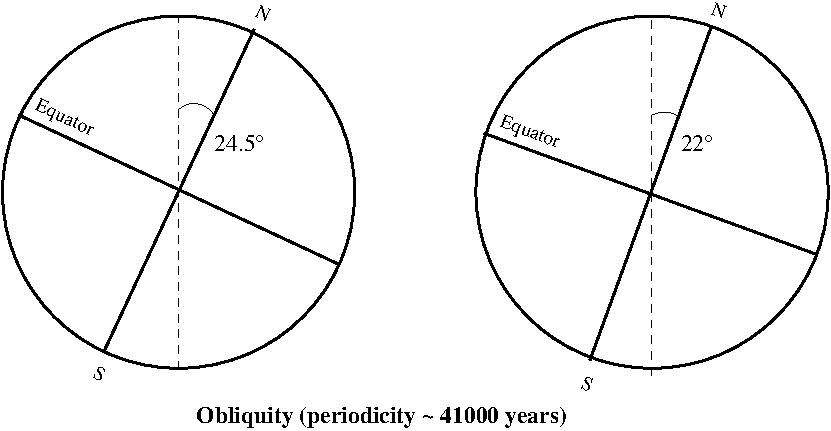
\includegraphics[width=12cm]{science/obliquity.pdf}
\else
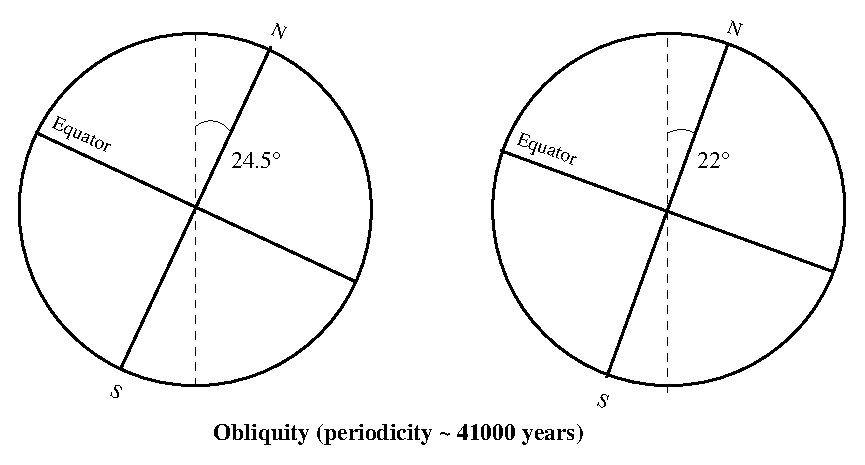
\includegraphics[width=12cm]{science/obliquity.eps}
\fi
\]
\caption{Obliquity}
\end{figure}

Obliquity does not influence the total amount of solar radiation
received by the Earth, but affects the distribution of insolation in
space and time. As obliquity increases, so does the amount of solar
radiation received at high latitudes in summer, whilst insolation
decreases in winter. Changes in obliquity have little effect at low
latitudes, since the strength of the effect decrease towards the
equator. Consequently, variations in the Earth's axial tilt affect the
strength of the latitudinal temperature gradient. Increased tilt has
the effect of raising the annual receipt of solar energy at high
latitudes, with a consequent reduction in the latitudinal temperature
gradient.

\subsection{Eccentricity}

The Earth's orbit around the Sun is not perfectly circular but follows
an elliptical path (see Figure \ref{eccentricity}). A second orbital
variation involves the strength of the ellipse, or eccentricity. This
parameter, $e$, is determined by Equation \ref{ecccalc}.

\begin{equation}
e = \frac{1}{2} \frac{(a^2 - b^2)}{a} 
\label{ecccalc}
\end{equation}

When the orbit is circular, the semimajor axis $a$ and semiminor axis
$b$ are equal and $e = 0$. The Earth's orbit has been found to vary
from being near circular ($e = 0.005$) to markedly elliptical ($e =
0.06$) with two primary periodicities of approximately 96000 and
413000 years \citep{berger76}. The current value of $e$ is 0.0167
\citep{meeus98}. Variations in eccentricity
influence the total amount of solar radiation incident at the top of
the Earth's atmosphere. With maximum eccentricity, differences in
solar radiation receipt of about 30 \% may occur between perihelion
and aphelion \citep{goodess92}.

\begin{figure}[htb]
\[
\ifpdf
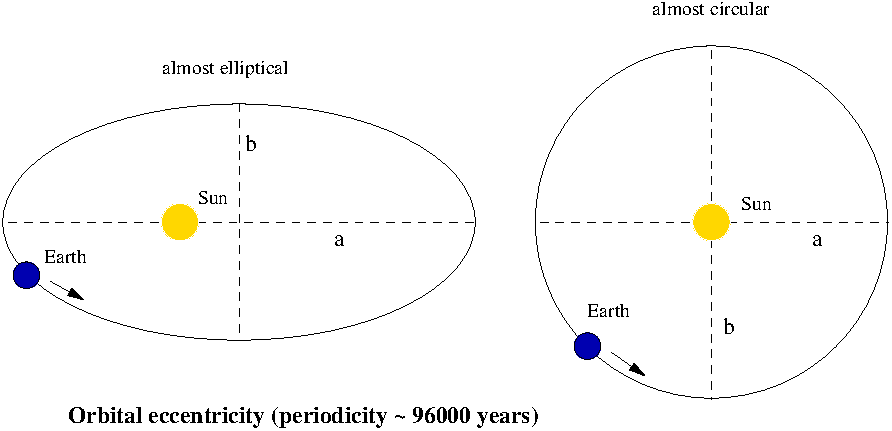
\includegraphics[width=12cm]{science/eccentricity.pdf}
\else
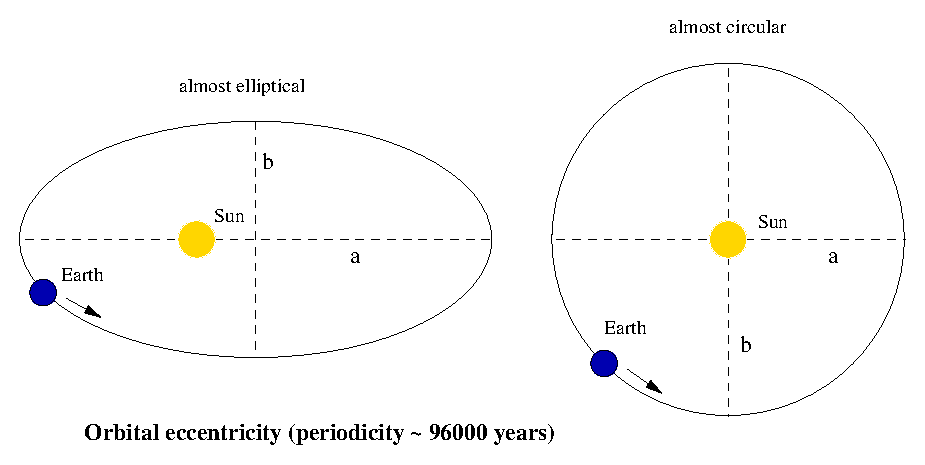
\includegraphics[width=12cm]{science/eccentricity.eps}
\fi
\]
\caption{\label{eccentricity}Eccentricity}
\end{figure}

\subsection{Precession}

The third orbital variation is that of precession. The Sun lies at one
of the focal points of the Earth's orbital ellipse. Due to the
gravitational interaction of other planetary bodies in the solar
system, primarily the Moon and the planet Jupiter, the perihelion (the
point at which the Earth passes closest to the Sun) moves in space
with a consequent shifting or precessing of the elliptical orbit. This
phenomenon is known as the precession of the equinoxes, and effects
the intensity of the seasons.

\begin{figure}[htb]
\[
\ifpdf
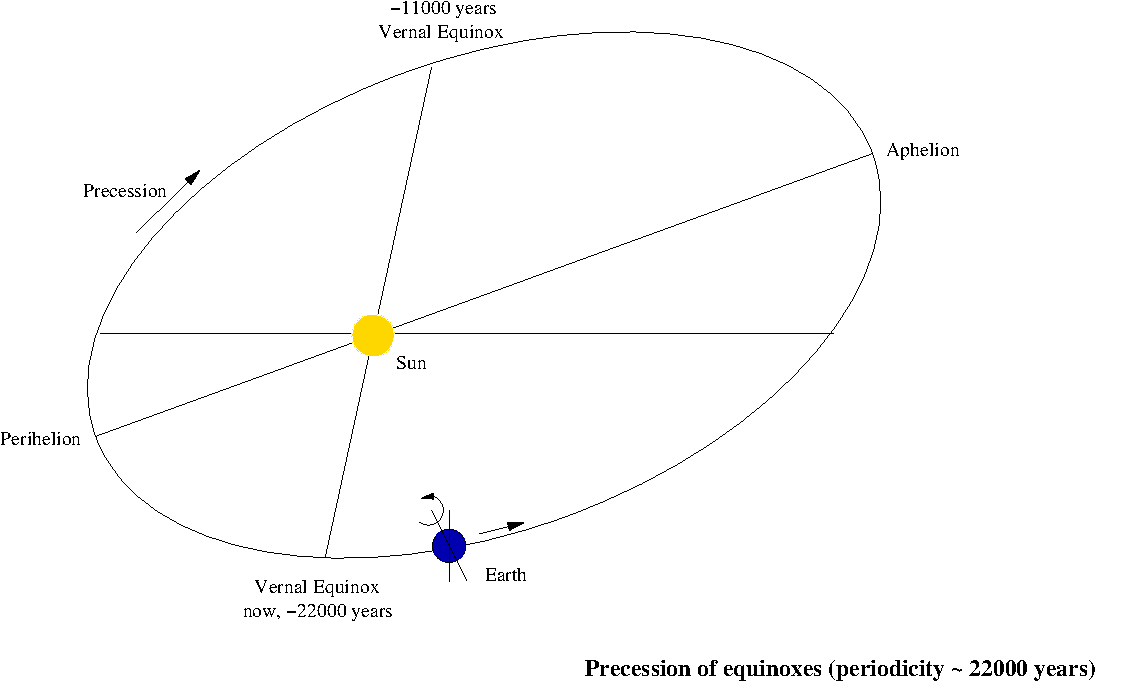
\includegraphics[width=12cm]{science/precession.pdf}
\else
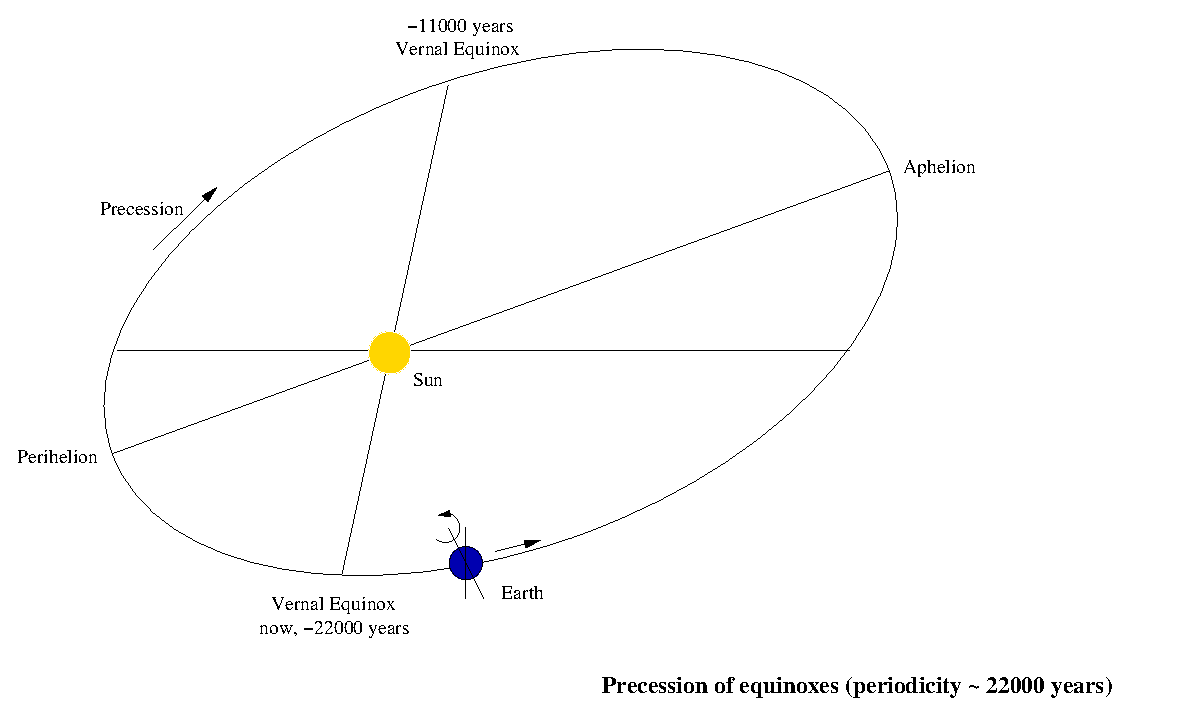
\includegraphics[width=12cm]{science/precession.eps}
\fi
\]
\caption{Precession}
\end{figure}

Precession has two components: an axial precession, in which the
torque of the other planets exerted on the Earth's equatorial bulge
causes the rotational axis to gyrate like a spinning top, and an
elliptical precession, in which the elliptical orbit of the Earth
itself rotates about one focus. The net effect describes the
precession of the equinoxes with a period of 22000 years. This term is
modulated by eccentricity which splits the precession into periods,
of 19000 and 23000 years \citep{crowell91}.

Like obliquity, precession does not affect the total amount of solar
energy received by the Earth, but only its hemispheric distribution
over time. If the perihelion occurs in mid-June i.e. when the Northern
Hemisphere is tilted toward the Sun, then the receipt of summer solar
radiation in Northern Hemisphere will increase. Conversely, if the
perihelion occurs in December, the Northern Hemisphere will receive
more solar radiation in winter. It should be clear that the direction
of changes in solar radiation receipt at the Earth's surface is
opposite in each hemisphere.


\section{Precise orbit determination based on VSOP87}

\subsection{VSOP --- Variations S\'{e}culaires des Orbites Plan\'{e}taires}

From an analytical solution of the motion of the planets expressed
with elliptic elements \citep{bretagnon82} the position of planets is
expressed as a Poisson series expansion. Different sets of coordinate
representations have been derived. The solution used in \echam for the
position of Earth is based on heliocentric spherical coordinate
variables and the reference frame is the mean equinox and ecliptic of
date.

The position of Earth is given by the heliocentric latitude $L$ and
longitude $B$ and the distance from the Sun $R$.

This coordinates are given by the following Poisson series:

\begin{eqnarray}
L & = & \sum_{n=1}^6 L_n \sum_{k=1}^{k_N} a_{k_n} \cos(b_{k_n}+c_{k_n} \tau^n) \\
B & = & \sum_{n=1}^2 B_n \sum_{k=1}^{k_N} a_{k_n} \cos(b_{k_n}+c_{k_n} \tau^n) \\
R & = & \sum_{n=1}^5 R_n \sum_{k=1}^{k_N} a_{k_n} \cos(b_{k_n}+c_{k_n} \tau^n) 
\end{eqnarray}

where $\tau$ is reckoned in thousands of Julian years from epoch J2000.0

\begin{equation}
\tau = \frac{\mbox{Julian date} - 2 451 545}{365 250}
\end{equation} 

The coefficients for the Poisson series expansions are given in tables
\ref{tab:L1} till \ref{tab:R5} in appendix \ref{app:orbit_tables}.

To derive the required coordinates of the Sun with respect to Earth
the calculated heliocentric spehrical coordinates have to be
transformed to geocentric spherical coordinates.

First step is a transformation of the Sun's and Earth's position to
heliocentric rectangular coordinates with:

\begin{equation}
\vec{X}_s = f(L_s,B_s,R_s) \quad \mbox{and} \quad  \vec{X}_e= f(L_e,B_e,R_e)
\end{equation}

$\vec{X}$ are the heliocentric rectangular coordinates, $(L,B,R)$ are the
heliocentric spherical coordinates. The subscripts $s$ and $e$ are
denoting the Sun and Earth respectively. The transformation function
$f$ is given by:

\begin{eqnarray}
X & = & R \cos L \cos B \nonumber \\
Y & = & R \sin L \cos B \label{str}\\
Z & = & R \sin B        \nonumber
\end{eqnarray}

The geocentric rectangular coordinates are than given by:

\begin{equation}
\vec{x} = \vec{X}_s - \vec{X}_e
\end{equation}

$\vec{x}$ has to be transformed to geocentric spherical coordinates by
the inverse $f^{-1}$ of equation \ref{str}:

\begin{eqnarray}
l & = & \arctan \frac{y}{x}  
	  \quad \mbox{with} \quad l = l + 2 \pi 
          \quad \mbox{for}  \quad l < 0 \\ \nonumber
b & = & \arcsin \frac{z}{r} \\
r & = & \sqrt{x^2+y^2+z^2} \nonumber
\end{eqnarray}

The next step is the transformation from the ecliptic geocentric to
equatorial geocentric coordinates. This requires the obliquity (or
inclination) $i$ of Earth.  This is a slowly varying property of the
Earth's orbit, see section \ref{obl}. For the calculation of the
actual obliquity a polynomial series developed by \cite{laskar93} is
used:

\begin{eqnarray}
i & = &   84381.448     \\ \nonumber
  &   & - 4680.93 U - 1.55 U^2 + 1999.25 U^3 - 51.38 U^4  - 249.67 U^5 \\ \nonumber 
  &   & -   39.05 U^6 + 7.12 U^7 +   27.87 U^8  +  5.79 U^9  +   2.45 U^10
\end{eqnarray}

$U$ is the time given as $U = 0.01 \tau$. The transformation to
equatorial geocentric coordinates is given by:

\begin{eqnarray}
\alpha  & = & \arctan \left(\frac{\cos b \sin l \cos i 
             - \sin b \sin i}{\cos b \cos L}\right)
	      \quad \mbox{with} \quad \alpha = \alpha + 2 \pi 
              \quad \mbox{for}  \quad \alpha < 0 \\ \nonumber
\delta  & = & \arcsin \left(\sin b \cos i + \cos b \sin i \sin l\right)
\end{eqnarray} 

There is another effect which has to be considered in determining the
Sun's position in geocentric coordinates and this is the aberration.
Aberration is the angular discrepancy between the apparent position of
a star and its true position, arising from the motion of an observer
relative to the path of the beam of light observed. This motion is the
result of velocity components like the speed of the diurnal rotation
of the Earth and its orbital speed in revolving around the sun. The
change in Earth's position due to aberration regarding the Sun is
given by:

\begin{eqnarray}
\Delta \alpha & = & -9.93639\,10^{-5} 
                    \frac {\left( \cos \alpha \cos \lambda \cos i 
                   + \sin \alpha \sin \lambda\right) } {\cos \delta} \\
\Delta \delta & = & -9.93639\,10^{-5} \cos \lambda \left( \sin i \cos \delta 
                   - \sin \alpha \sin\delta \cos i\right) 
                   + \cos \alpha \sin \delta \sin \lambda
\end{eqnarray}

where $\lambda$ is the longitude and $e$ the eccentricity of the Sun 
given by

\begin{equation}
\lambda = L_0 + C 
\end{equation}

where $L_0$ is the Sun's longitude of the ascending node, and $C$ the
position of the Sun, these are in terms of mean anomaly $M$ and
eccentricity $e$ (in degrees), and time $t$ in hundreds of Julian
years:

\begin{eqnarray}
L_0 & = & 280.46646 + 36000.76983 \, t + 0.0003032 \, t^2                  \\
M   & = & 357.52910 + 35999.05028 \, t - 0.0001561 \, t^2                  \\
e   & = & 0.016708617 - 0.000042040 \, t + 0.0000001236 \, t^2             \\ 
    &   & \\ \nonumber
C   & = & e \, (2-0.25 \, e^2) \sin M 
                + 1.25 \, e^2 \sin 2M 
                + 1.083 \, e^3 \sin 3M
\end{eqnarray}

with

\[
t = \frac{\mbox{Julian date} - 2451545}{36525}
\]

So, the final position is 

\begin{eqnarray}
\alpha & = & \alpha + \Delta \alpha \\
\delta & = & \delta + \Delta \delta
\end{eqnarray}

Finaly the mean sidereal time in degrees has to be determined:

\begin{eqnarray}
\theta_0 & = & \left( 280.46061837 
                + 360.98564736629 \cdot 36525 \, t 
                + 0.000387933 \, t^2 
                - \frac{t^3}{38710000}\right) \\ \nonumber
& & \quad \mbox{with} \theta_0 = \theta_0 \mbox{mod} 360
\end{eqnarray}

\subsection{Nutation}

Nutation is a small wobble of the Earth's rotational axis with an
amplitude of about 9 arcsec and period of up to 18.6 years.
Traditionally, nutation is represented by variations in ecliptic
longitude and obliquity (the angle between the ecliptic and the
equator). Current models represent the nutation quantities with
well-defined series \citep{seidelmann82}.

The nutation of the Earth is handled by the following equations and
added before the transformation from the geocentric ecliptic to the
geocentric equatorial coordinate system is performed.

Five auxilliar variables must be calculated which allows the further
expansion of a sine/cosine series for the nutation. The five variables 
are

\begin{itemize}
\item longitude of the mean ascending node of the lunar orbit
      on the ecliptic, measured from the mean equinox of date
      \begin{equation}
      \Omega =   125.0445222 -   1934.1362608 \, t + 0.00207833 \, t^2 + 2.220e-6 \, t^3
      \end{equation}
\item mean longitude of the Sun minus the mean longitude of the Sun's perigee
      \begin{equation}
      M      =   357.5277233 +  35999.0503400 \, t - 0.00016030 \, t^2 - 3.330e-6 \, t^3
      \end{equation}
\item mean longitude of the Moon minus the mean longitude of the Moon's perigee
      \begin{equation}
      M'     =   134.9629814 + 477198.8673981 \, t + 0.00869720 \, t^2 + 1.778e-5 \, t^3
      \end{equation}
\item mean longitude of the Moon minus the mean longitude of the Moon's node
      \begin{equation}
      F      =    93.2719103 + 483202.0175381 \, t - 0.00368250 \, t^2 + 3.056e-6 \, t^3
      \end{equation}
\item mean elongation of the Moon from the Sun
      \begin{equation}
      D      =   297.8503631 + 445267.1114800 \, t - 0.00191420 \, t^2 + 5.278e-6 \, t^3
      \end{equation}
\end{itemize}

The table \ref{tab:nut} with the require coeeficients is given in
appendix \ref{app:orbit_tables}.

\section{Kepler based orbit for paleoclimate applications}

The three components of the orbital variations, obliquity,
eccentricity, and precession together effect both the total flux of
incoming solar radiation and also the temporal and spatial
distribution of terrestrial insolation. These variations have the
potential to influence the energy budget of the climate system
\citep{milankovitch41,berger78}, and can therefore be regarded as
possible causes of climate change over long time scales.

\cite{milankovitch41} considered the changing seasonal (precession) and
latitudinal (obliquity) patterns of incoming radiation to be critical
factors in the growth of continental ice sheets and in the initiation
of ice ages. He hypothesised that when axial tilt was small (large
latitudinal temperature gradient), eccentricity was large and
perihelion occurred during the Northern Hemisphere winter (warmer
winters and colder summers), such a configuration would allow the
persistence of accumulated snow throughout the summer months in the
Northern Hemisphere. Additionally, the warmer winters and stronger
atmospheric general circulation due to the increased temperature
gradient would increase the amount of water vapour at the high
latitudes available for snowfall.

To allow for paleoclimate studies, \echam provides an Kepler based
orbit which has as basic parameters, to be defined externally, the
long term varying orbit parameters obliquity, eccentricity, and, as
measure for the precession, the longitude of perihelion from the
equinox of date.

Used for the calculation of the position of the Sun is Lacaille's formula
which links the true anomaly $\nu$ and the eccentric anomaly $E$:

\begin{equation}
\tan\frac{\nu}{2} = \sqrt{\frac{1+e}{1-e}}\tan\frac{E}{2}
\label{lacaille}
\end{equation} 

with $\nu = \omega$, where $\omega$ is the longitude of perihelion. This allows
the calculation of the eccentric anomaly which is required for the Kepler 
equation linking the eccentric and the mean anomaly $M$:

\begin{equation}
\label{kepler}
M = E - e \sin E
\end{equation}

First, calculate the mean anomaly $M$ of the current longitude
$\lambda$ from the true anomaly $\nu$:

\begin{equation}
M = \lambda - M(\omega) \quad \mbox{with} \quad M(\omega) = \nu - e \sin \nu  
\end{equation}

The true and mean anomaly are identical at the vernal equinox. For
solving the Kepler equation \ref{kepler} the Newton method is used:

\[
E^{m+1} = E^m - \frac{K(E^m)}{K'(E^m)} 
\]

with

\[
K(E) = M - E + e \sin E = 0 \quad \mbox{and} \quad K'(E) = 1 + e \cos E
\]

so the final iteration expression to solve is:

\begin{equation}
E^{m+1} = E^m - \frac{M - E^m + e \sin E^m}{1 + e \cos E^m}
\end{equation}
	
This iterative solver does converge for most initial values, but not for
all. This has been taken into account. For more details see \cite{meeus98}.

The final distance between Earth and Sun is given by 

\begin{equation}
R = \left(\frac{1}{1-e \cos E}\right)^2
\end{equation}

and the true anomaly $\nu$ with Lacaille's formula (equation \ref{lacaille}).
The true longitude is $\lambda = \nu + \omega$ and the declination of the
Sun (with $i$ the obliquity (or inclination):

\begin{equation}
\delta = \sin i \sin \lambda
\end{equation}

and the right ascension:

\begin{equation}
\alpha = \tan \frac{\cos i \sin \lambda}{\cos \lambda}
\end{equation}

\section{Differences in the daily insolation due to the two given orbits}

The astronomical orbital parameters have to be transformed into
the solar constant scaled by the distance Earth --- Sun $R$
and the local zenith angle $Z$.

For comparison of the two given orbits the difference in the 
orbit parameters against the JPL DE405 are shown. The first set
is for the AMIP2 period 1978 to 1996 and the second set for 
1870 till 2150.

\begin{figure}[htb]
\begin{center}
\ifpdf
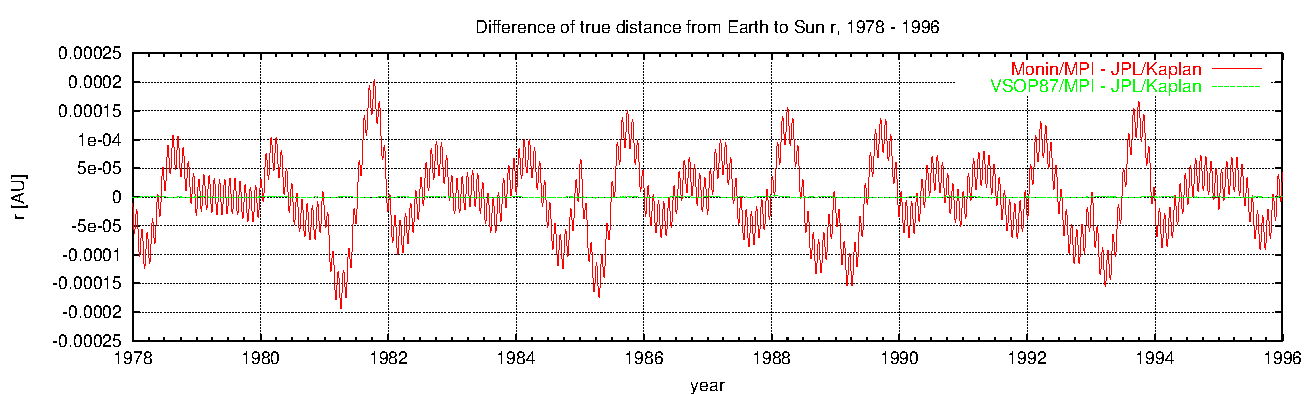
\includegraphics[width=15cm]{science/dis_1978-1996.pdf}

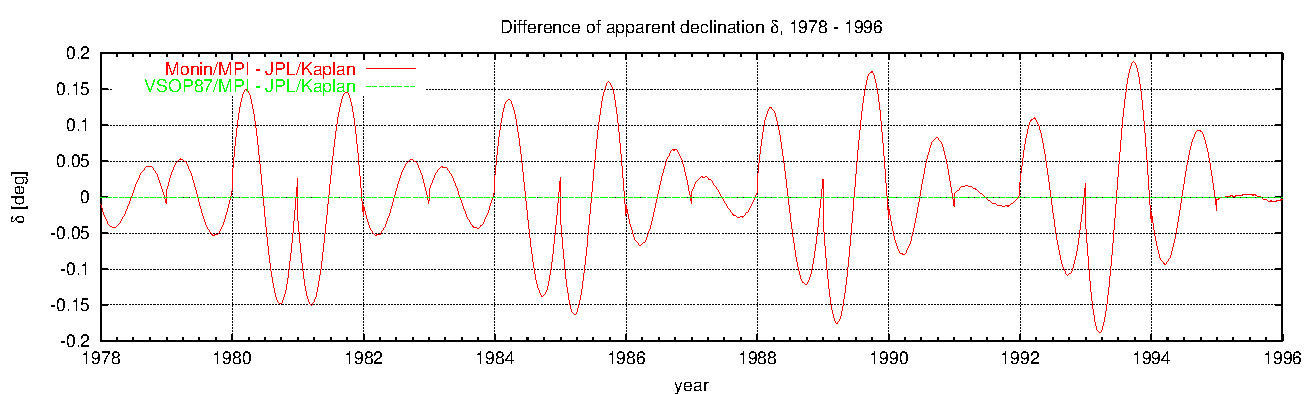
\includegraphics[width=15cm]{science/dec_1978-1996.pdf}

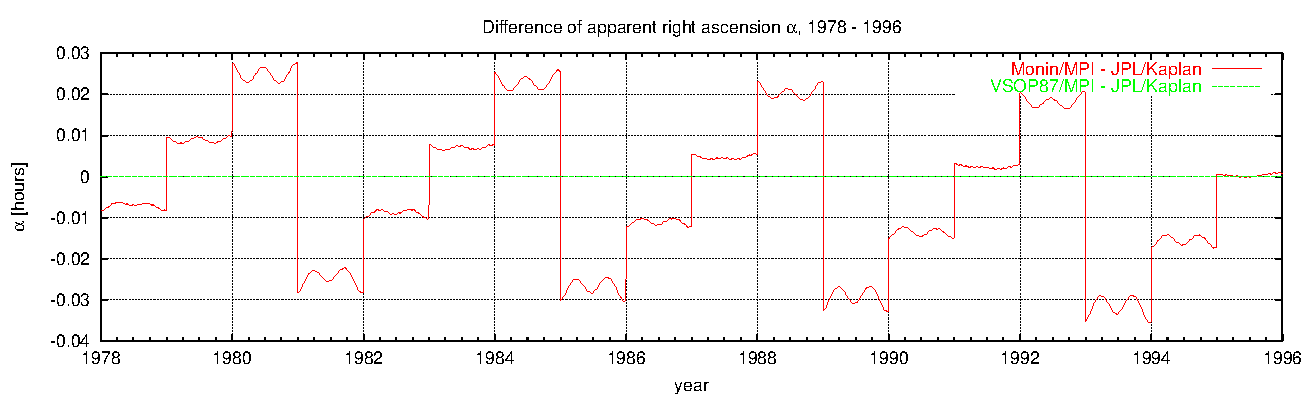
\includegraphics[width=15cm]{science/ra_1978-1996.pdf}

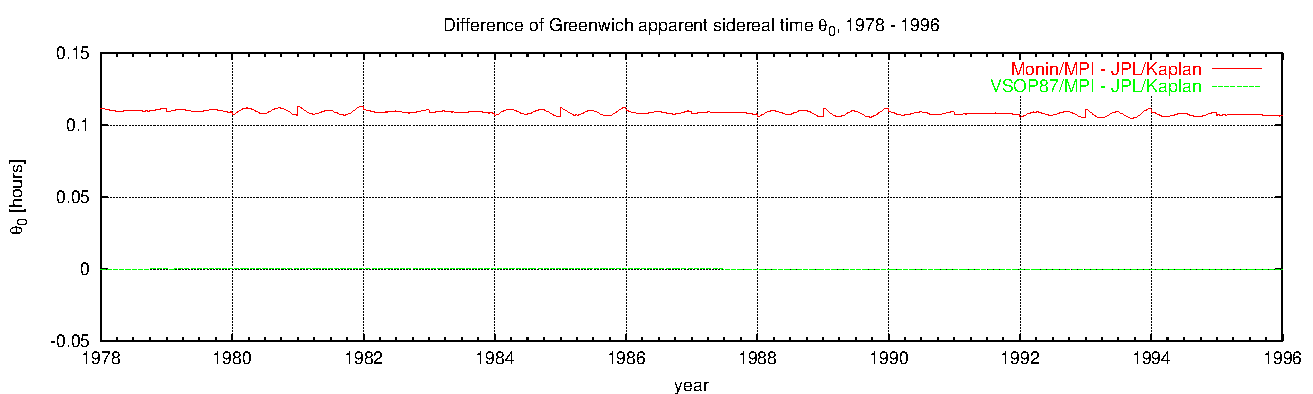
\includegraphics[width=15cm]{science/ga_1978-1996.pdf}
\else
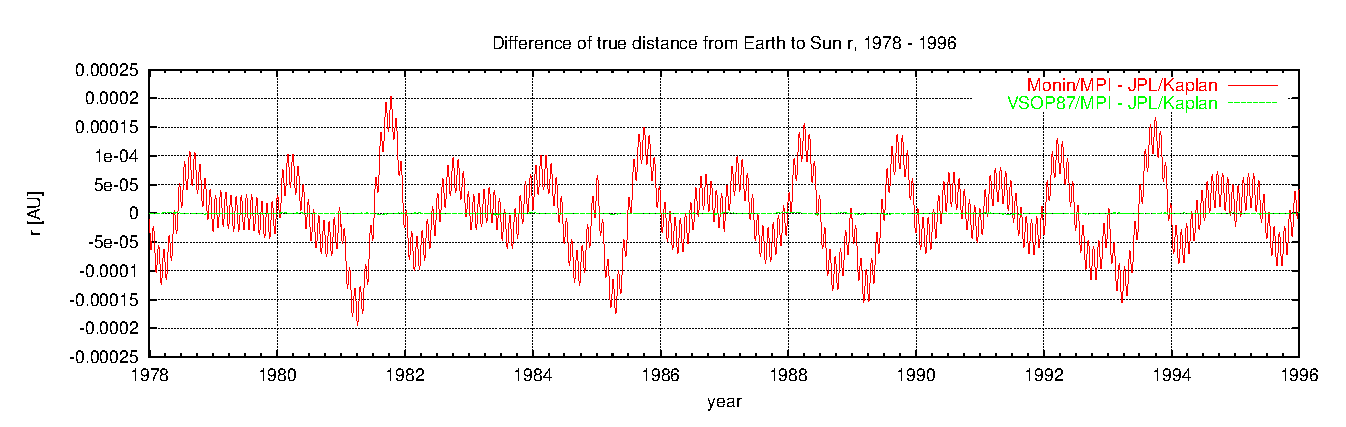
\includegraphics[width=15cm]{science/dis_1978-1996.ps}

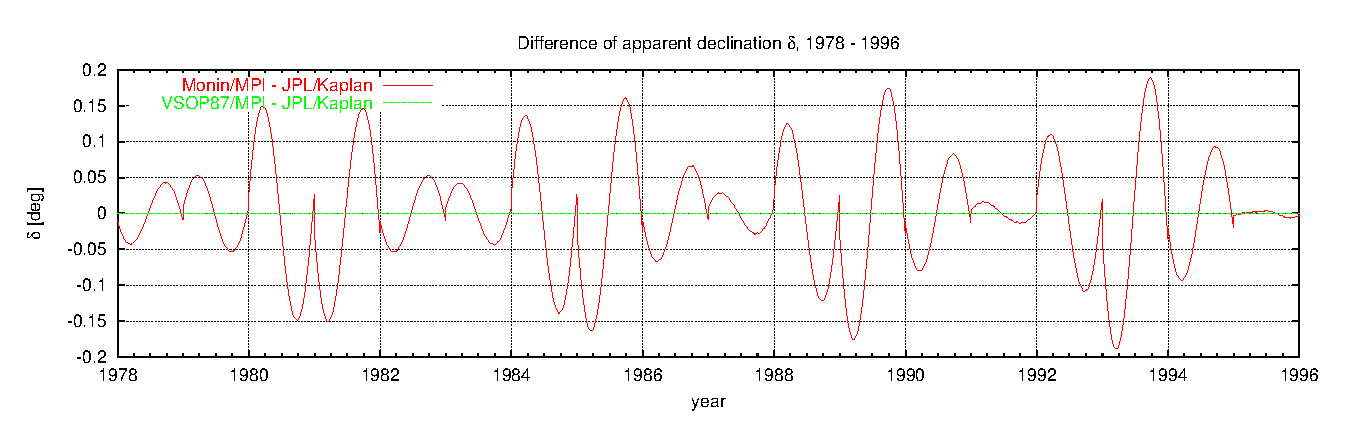
\includegraphics[width=15cm]{science/dec_1978-1996.ps}

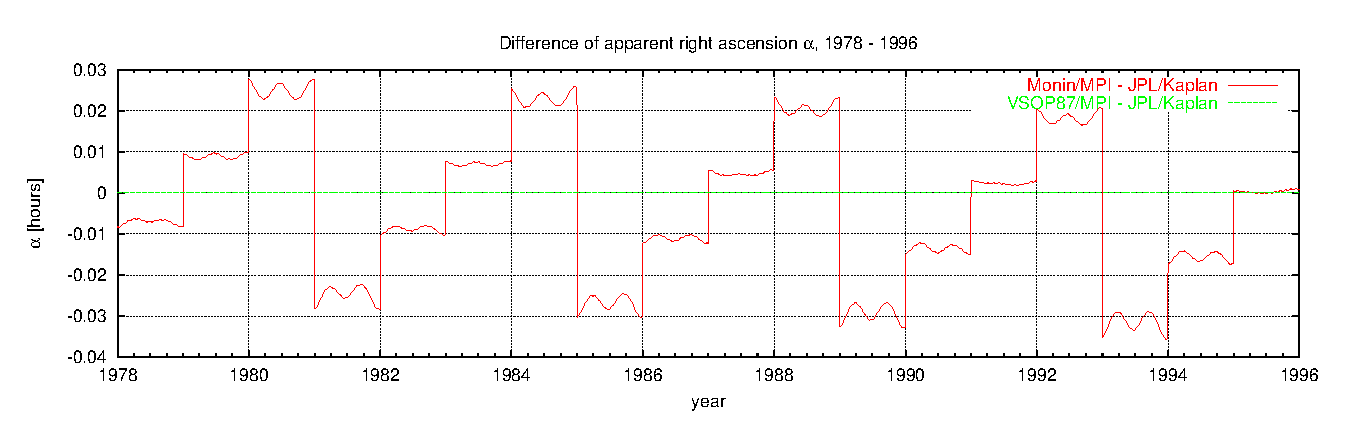
\includegraphics[width=15cm]{science/ra_1978-1996.ps}

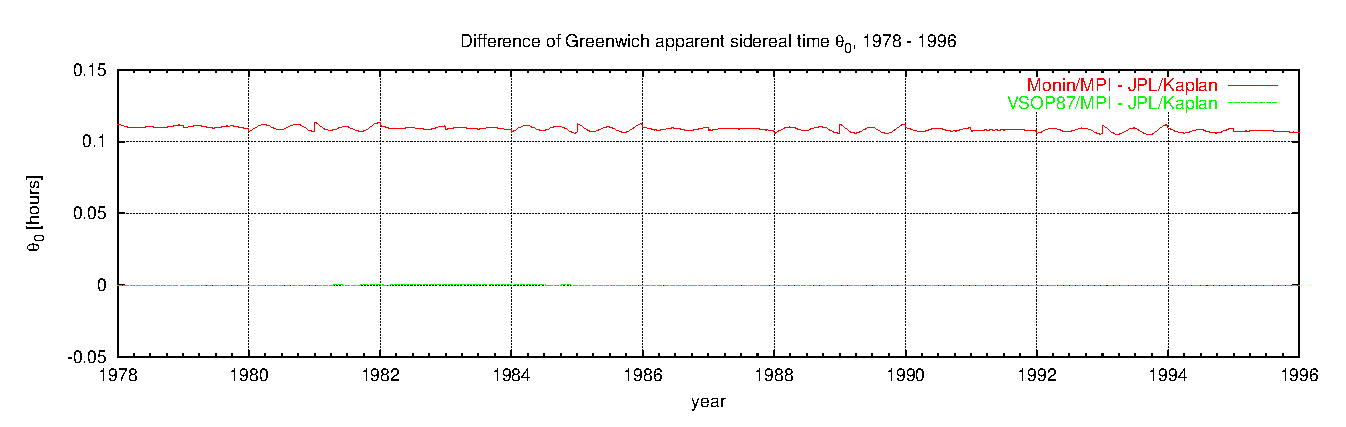
\includegraphics[width=15cm]{science/ga_1978-1996.ps}
\fi
\end{center}
\caption{Differences between the VSOP87 and Monin orbit with respect to JPL's DE405 for the peride 1978 till 1996}
\end{figure}

\begin{figure}[htb]
\begin{center}
\ifpdf
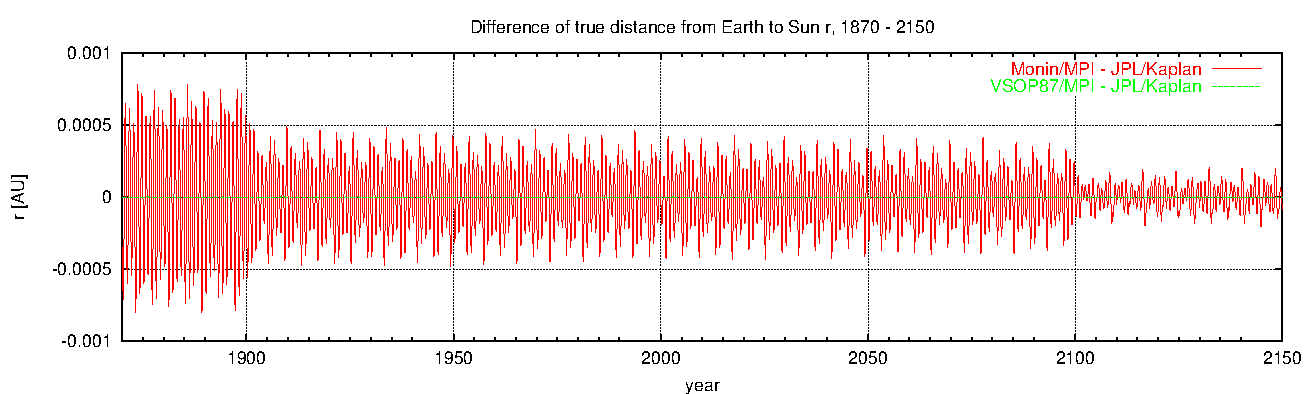
\includegraphics[width=15cm]{science/dis_1870-2150.pdf}

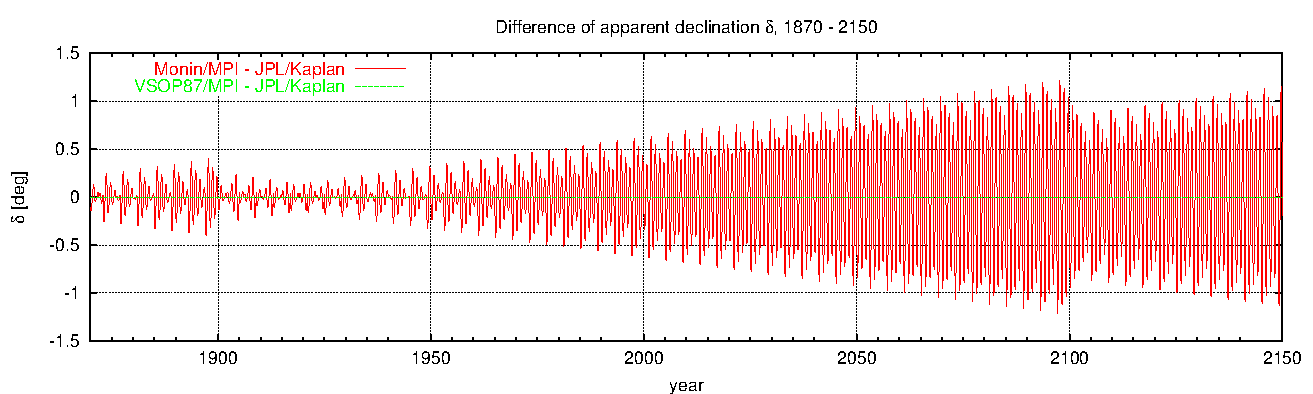
\includegraphics[width=15cm]{science/dec_1870-2150.pdf}

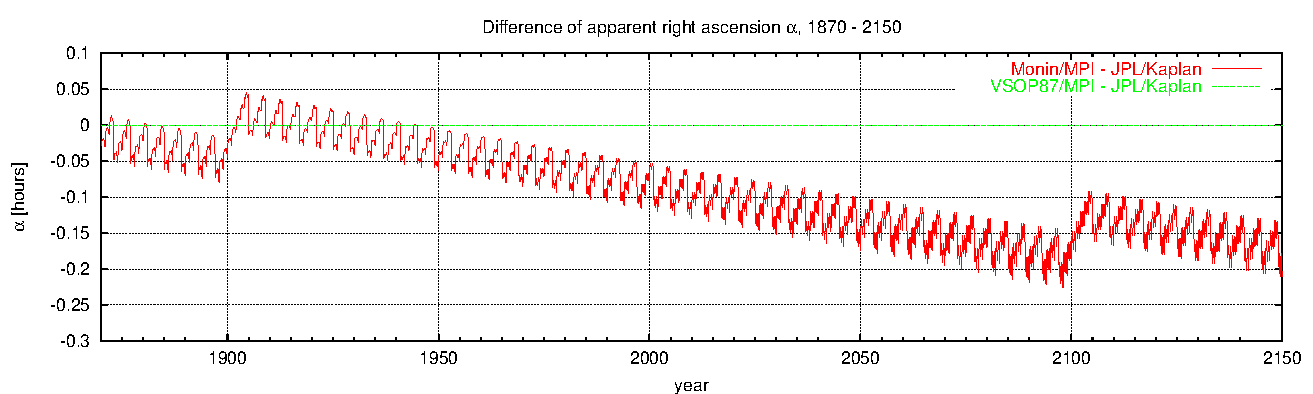
\includegraphics[width=15cm]{science/ra_1870-2150.pdf}

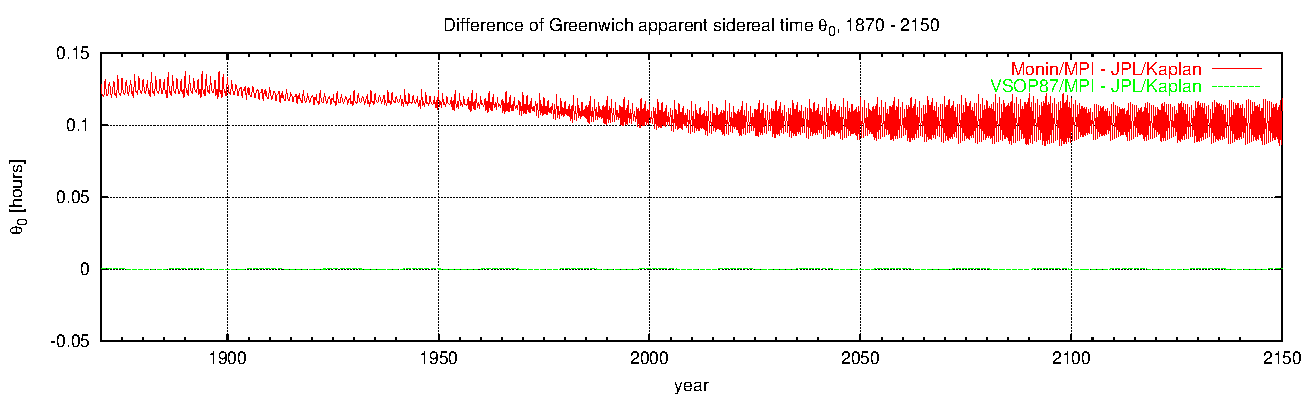
\includegraphics[width=15cm]{science/ga_1870-2150.pdf}
\else
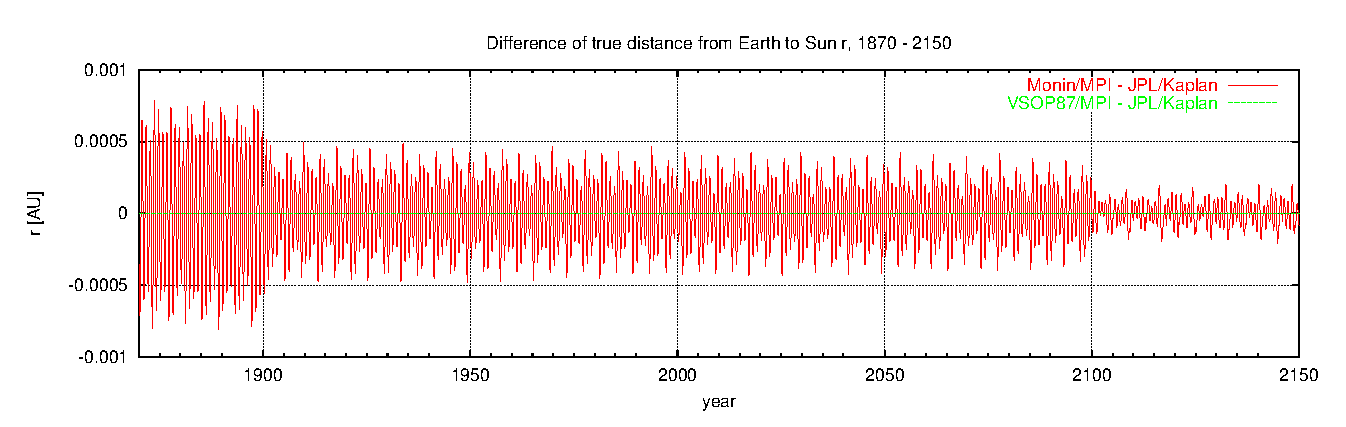
\includegraphics[width=15cm]{science/dis_1870-2150.ps}

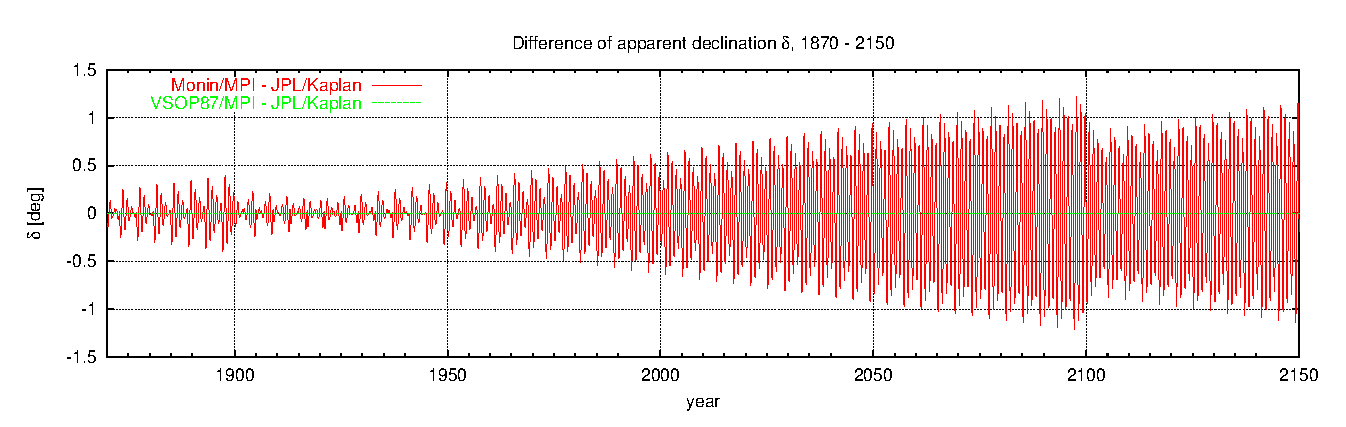
\includegraphics[width=15cm]{science/dec_1870-2150.ps}

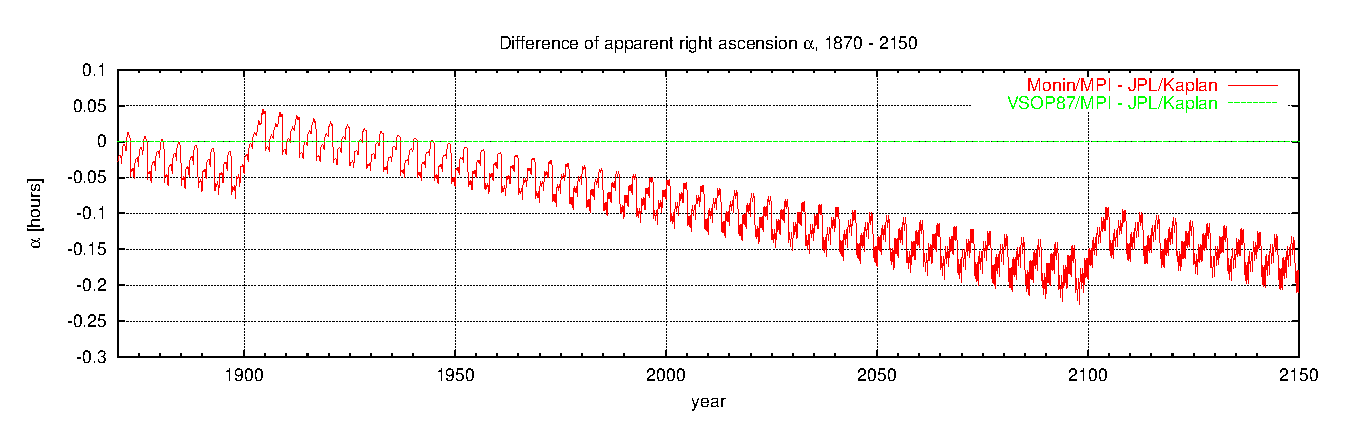
\includegraphics[width=15cm]{science/ra_1870-2150.ps}

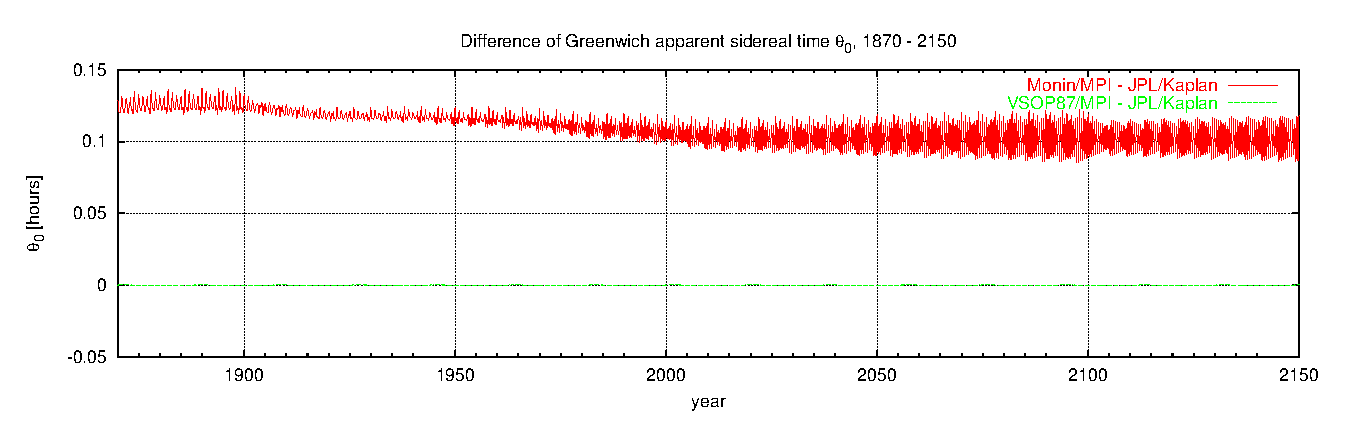
\includegraphics[width=15cm]{science/ga_1870-2150.ps}
\fi
\end{center}
\caption{Differences between the VSOP87 and Monin orbit with respect to JPL's DE405 for the peride 1870 till 2150}
\end{figure}

\parskip 1ex minus 0.2ex
\section{Orbit tables}\label{app:orbit_tables}

The coefficients for the Poisson series expansions required for the
VSOP87 orbit calculation.

\small

%-----------------------------------------------------------------------------
\bottomcaption{First summand of heliocentric latitude (VSOP87D)} \label{tab:L1}
%
\tablehead{\hline
\multicolumn{3}{|l|}{L1} \\ \hline
$a_k$ & $b_k$ & $c_k$    \\ \hline \hline}
%
\tabletail{\hline \hline
\multicolumn{3}{|l|}{table \ref{tab:L1} to be continued $\ldots$} \\ \hline}
\tablelasttail{\hline \hline}
%-----------------------------------------------------------------------------
\begin{center}
\texttt{
\begin{xtabular}{|l|l|l|}
1.753470456730000e+00 & 0.00000000000e+00 & 0.000000000000000e+00 \\ 
3.341656456000000e-02 & 4.66925680417e+00 & 6.283075849991400e+03 \\ 
3.489427500000000e-04 & 4.62610241759e+00 & 1.256615169998280e+04 \\ 
3.497056000000000e-05 & 2.74411800971e+00 & 5.753384884896800e+03 \\ 
3.417571000000000e-05 & 2.82886579606e+00 & 3.523118349000000e+00 \\ 
3.135896000000000e-05 & 3.62767041758e+00 & 7.771377146812050e+04 \\ 
2.676218000000000e-05 & 4.41808351397e+00 & 7.860419392439200e+03 \\ 
2.342687000000000e-05 & 6.13516237631e+00 & 3.930209696219600e+03 \\ 
1.324292000000000e-05 & 7.42463563520e-01 & 1.150676976979360e+04 \\ 
1.273166000000000e-05 & 2.03709655772e+00 & 5.296909650946000e+02 \\ 
1.199167000000000e-05 & 1.10962944315e+00 & 1.577343542447800e+03 \\ 
9.902500000000000e-06 & 5.23268129594e+00 & 5.884926846583200e+03 \\ 
9.018550000000000e-06 & 2.04505443513e+00 & 2.629831979980000e+01 \\ 
8.572229999999999e-06 & 3.50849156957e+00 & 3.981490034082000e+02 \\ 
7.797859999999999e-06 & 1.17882652114e+00 & 5.223693919802200e+03 \\ 
7.531410000000000e-06 & 2.53339053818e+00 & 5.507553238667400e+03 \\ 
5.052640000000000e-06 & 4.58292563052e+00 & 1.884922754997420e+04 \\ 
4.923790000000000e-06 & 4.20506639861e+00 & 7.755226113240000e+02 \\ 
3.566550000000000e-06 & 2.91954116867e+00 & 6.731030280000000e-02 \\ 
3.170870000000000e-06 & 5.84901952218e+00 & 1.179062908865880e+04 \\ 
2.841250000000000e-06 & 1.89869034186e+00 & 7.962980068163999e+02 \\ 
2.710390000000000e-06 & 3.14886076490e-01 & 1.097707880469900e+04 \\ 
2.428100000000000e-06 & 3.44811409060e-01 & 5.486777843175000e+03 \\ 
2.061600000000000e-06 & 4.80646606059e+00 & 2.544314419883400e+03 \\ 
2.053850000000000e-06 & 1.86947813692e+00 & 5.573142801433100e+03 \\ 
2.022610000000000e-06 & 2.45767795458e+00 & 6.069776754553400e+03 \\ 
1.555160000000000e-06 & 8.33060738070e-01 & 2.132990954380000e+02 \\ 
1.322120000000000e-06 & 3.41118275555e+00 & 2.942463423291600e+03 \\ 
1.261840000000000e-06 & 1.08302630210e+00 & 2.077539549240000e+01 \\ 
1.151320000000000e-06 & 6.45449116830e-01 & 9.803210682000000e-01 \\ 
1.028510000000000e-06 & 6.35998467270e-01 & 4.694002954707600e+03 \\ 
1.018950000000000e-06 & 9.75692218240e-01 & 1.572083878487840e+04 \\ 
1.017240000000000e-06 & 4.26679821365e+00 & 7.113547000800000e+00 \\ 
9.920600000000000e-07 & 6.20992940258e+00 & 2.146165416475200e+03 \\ 
9.760700000000001e-07 & 6.81012722700e-01 & 1.554203994342000e+02 \\ 
8.580300000000000e-07 & 5.98322631256e+00 & 1.610006857376741e+05 \\ 
8.512800000000000e-07 & 1.29870743025e+00 & 6.275962302990600e+03 \\ 
8.471100000000000e-07 & 3.67080093025e+00 & 7.143069561812909e+04 \\ 
7.963700000000000e-07 & 1.80791330700e+00 & 1.726015465469040e+04 \\ 
7.875600000000000e-07 & 3.03698313141e+00 & 1.203646073488820e+04 \\ 
7.465100000000000e-07 & 1.75508916159e+00 & 5.088628839766800e+03 \\ 
7.387400000000000e-07 & 3.50319443167e+00 & 3.154687084895600e+03 \\ 
7.354700000000000e-07 & 4.67926565481e+00 & 8.018209311238001e+02 \\ 
6.962700000000000e-07 & 8.32975969660e-01 & 9.437762934887000e+03 \\ 
6.244899999999999e-07 & 3.97763880587e+00 & 8.827390269874801e+03 \\ 
6.114800000000000e-07 & 1.81839811024e+00 & 7.084896781115200e+03 \\ 
5.696300000000000e-07 & 2.78430398043e+00 & 6.286598968340400e+03 \\ 
5.611600000000000e-07 & 4.38694880779e+00 & 1.414349524243060e+04 \\ 
5.557700000000000e-07 & 3.47006009062e+00 & 6.279552731642400e+03 \\ 
5.199200000000000e-07 & 1.89149458340e-01 & 1.213955350910680e+04 \\ 
5.160500000000000e-07 & 1.33282746983e+00 & 1.748016413067000e+03 \\ 
5.114500000000000e-07 & 2.83068645010e-01 & 5.856477659115400e+03 \\ 
4.900000000000000e-07 & 4.87350650330e-01 & 1.194447010224600e+03 \\ 
4.103600000000000e-07 & 5.36817351402e+00 & 8.429241266466601e+03 \\ 
4.093800000000000e-07 & 2.39850881707e+00 & 1.965104848109800e+04 \\ 
3.920000000000000e-07 & 6.16832995016e+00 & 1.044738783960440e+04 \\ 
3.677000000000000e-07 & 6.04133859347e+00 & 1.021328554621100e+04 \\ 
3.659600000000000e-07 & 2.56955238628e+00 & 1.059381930189200e+03 \\ 
3.595400000000000e-07 & 1.70876111898e+00 & 2.352866153771800e+03 \\ 
3.556600000000000e-07 & 1.77597314691e+00 & 6.812766815086000e+03 \\ 
3.329100000000000e-07 & 5.93094994590e-01 & 1.778984561978500e+04 \\ 
3.041200000000000e-07 & 4.42944641350e-01 & 8.399684731811189e+04 \\ 
3.004700000000000e-07 & 2.73975123935e+00 & 1.349867409658800e+03 \\ 
2.535200000000000e-07 & 3.16470953405e+00 & 4.690479836358600e+03 \\
\end{xtabular}}
\end{center}
%-----------------------------------------------------------------------------
\bottomcaption{Second summand of heliocentric latitude (VSOP87D)} \label{tab:L2}
%
\tablehead{\hline
\multicolumn{3}{|l|}{L2} \\ \hline
$a_k$ & $b_k$ & $c_k$    \\ \hline \hline}
%
\tabletail{\hline \hline
\multicolumn{3}{|l|}{table \ref{tab:L2} to be continued $\ldots$} \\ \hline}
\tablelasttail{\hline \hline}
%----------------------------------------------------------------------------
\begin{center}
\texttt{
\begin{xtabular}{|l|l|l|}
6.283319667474910e+03 & 0.00000000000e+00 & 0.000000000000000e+00 \\ 
2.060588630000000e-03 & 2.67823455584e+00 & 6.283075849991400e+03 \\ 
4.303430000000000e-05 & 2.63512650414e+00 & 1.256615169998280e+04 \\ 
4.252640000000000e-06 & 1.59046980729e+00 & 3.523118349000000e+00 \\ 
1.192610000000000e-06 & 5.79557487799e+00 & 2.629831979980000e+01 \\ 
1.089770000000000e-06 & 2.96618001993e+00 & 1.577343542447800e+03 \\ 
9.347800000000000e-07 & 2.59212835365e+00 & 1.884922754997420e+04 \\ 
7.212200000000000e-07 & 1.13846158196e+00 & 5.296909650946000e+02 \\ 
6.776800000000000e-07 & 1.87472304791e+00 & 3.981490034082000e+02 \\ 
6.732700000000000e-07 & 4.40918235168e+00 & 5.507553238667400e+03 \\ 
5.902700000000000e-07 & 2.88797038460e+00 & 5.223693919802200e+03 \\ 
5.597600000000000e-07 & 2.17471680261e+00 & 1.554203994342000e+02 \\ 
4.540700000000000e-07 & 3.98030798050e-01 & 7.962980068163999e+02 \\ 
3.636900000000000e-07 & 4.66247398350e-01 & 7.755226113240000e+02 \\ 
2.895800000000000e-07 & 2.64707383882e+00 & 7.113547000800000e+00 \\ 
2.084400000000000e-07 & 5.34138275149e+00 & 9.803210682000000e-01 \\ 
1.909700000000000e-07 & 1.84628332577e+00 & 5.486777843175000e+03 \\ 
1.850800000000000e-07 & 4.96855124577e+00 & 2.132990954380000e+02 \\ 
1.729300000000000e-07 & 2.99116864949e+00 & 6.275962302990600e+03 \\ 
1.623300000000000e-07 & 3.21648304700e-02 & 2.544314419883400e+03 \\ 
1.583200000000000e-07 & 1.43049285325e+00 & 2.146165416475200e+03 \\ 
1.461500000000000e-07 & 1.20532366323e+00 & 1.097707880469900e+04 \\ 
1.246100000000000e-07 & 2.83432285512e+00 & 1.748016413067000e+03 \\ 
1.187700000000000e-07 & 3.25804815607e+00 & 5.088628839766800e+03 \\ 
1.180800000000000e-07 & 5.27379790480e+00 & 1.194447010224600e+03 \\ 
1.151400000000000e-07 & 2.07502418155e+00 & 4.694002954707600e+03 \\ 
1.064100000000000e-07 & 7.66141992020e-01 & 5.535694028424000e+02 \\ 
9.969000000000000e-08 & 1.30262991097e+00 & 6.286598968340400e+03 \\ 
9.720999999999999e-08 & 4.23925472239e+00 & 1.349867409658800e+03 \\ 
9.452000000000000e-08 & 2.69957062864e+00 & 2.427286039740000e+02 \\ 
8.577000000000001e-08 & 5.64475868067e+00 & 9.517184062506000e+02 \\ 
7.576000000000000e-08 & 5.30062664886e+00 & 2.352866153771800e+03 \\ 
6.385000000000001e-08 & 2.65033984967e+00 & 9.437762934887000e+03 \\ 
6.101000000000000e-08 & 4.66632584188e+00 & 4.690479836358600e+03 \\
\end{xtabular}}
\end{center}
%-----------------------------------------------------------------------------
\bottomcaption{Third summand of heliocentric latitude (VSOP87D)} \label{tab:L3}
%
\tablehead{\hline
\multicolumn{3}{|l|}{L3} \\ \hline
$a_k$ & $b_k$ & $c_k$    \\ \hline \hline}
%
\tabletail{\hline \hline 
\multicolumn{3}{|l|}{table \ref{tab:L3} to be continued $\ldots$} \\ \hline}
\tablelasttail{\hline \hline}
%-----------------------------------------------------------------------------
\begin{center}
\texttt{
\begin{xtabular}{|l|l|l|}
5.291887000000000e-04 & 0.00000000000e+00 & 0.000000000000000e+00 \\ 
8.719837000000000e-05 & 1.07209665242e+00 & 6.283075849991400e+03 \\ 
3.091250000000000e-06 & 8.67288188320e-01 & 1.256615169998280e+04 \\ 
2.733900000000000e-07 & 5.29787169100e-02 & 3.523118349000000e+00 \\ 
1.633400000000000e-07 & 5.18826691036e+00 & 2.629831979980000e+01 \\ 
1.575200000000000e-07 & 3.68457889430e+00 & 1.554203994342000e+02 \\ 
9.541000000000001e-08 & 7.57422976750e-01 & 1.884922754997420e+04 \\ 
8.937000000000000e-08 & 2.05705419118e+00 & 7.771377146812050e+04 \\ 
6.952000000000000e-08 & 8.26733054100e-01 & 7.755226113240000e+02 \\ 
5.064000000000000e-08 & 4.66284525271e+00 & 1.577343542447800e+03 \\ 
4.061000000000000e-08 & 1.03057162962e+00 & 7.113547000800000e+00 \\ 
3.810000000000000e-08 & 3.44050803490e+00 & 5.573142801433100e+03 \\ 
3.463000000000000e-08 & 5.14074632811e+00 & 7.962980068163999e+02 \\ 
3.169000000000000e-08 & 6.05291851171e+00 & 5.507553238667400e+03 \\ 
3.020000000000000e-08 & 1.19246506441e+00 & 2.427286039740000e+02 \\ 
2.886000000000000e-08 & 6.11652627155e+00 & 5.296909650946000e+02 \\ 
2.714000000000000e-08 & 3.06378810250e-01 & 3.981490034082000e+02 \\ 
2.538000000000000e-08 & 2.27992810679e+00 & 5.535694028424000e+02 \\ 
2.371000000000000e-08 & 4.38118838167e+00 & 5.223693919802200e+03 \\ 
2.079000000000000e-08 & 3.75435330484e+00 & 9.803210682000000e-01 \\ 
\end{xtabular}}
\end{center}
%-----------------------------------------------------------------------------
\bottomcaption{Fourth summand of heliocentric latitude (VSOP87D)} \label{tab:L4}
%
\tablehead{\hline
\multicolumn{3}{|l|}{L4} \\ \hline
$a_k$ & $b_k$ & $c_k$    \\ \hline \hline}
%
\tabletail{\hline \hline 
\multicolumn{3}{|l|}{table \ref{tab:L4} to be continued $\ldots$} \\ \hline}
\tablelasttail{\hline \hline}
%-----------------------------------------------------------------------------
\begin{center}
\texttt{
\begin{xtabular}{|l|l|l|}
2.892260000000000e-06 & 5.84384198723e+00 & 6.283075849991400e+03 \\ 
3.495500000000000e-07 & 0.00000000000e+00 & 0.000000000000000e+00 \\ 
1.681900000000000e-07 & 5.48766912348e+00 & 1.256615169998280e+04 \\ 
2.962000000000000e-08 & 5.19577265202e+00 & 1.554203994342000e+02 \\ 
1.288000000000000e-08 & 4.72200252235e+00 & 3.523118349000000e+00 \\ 
7.140000000000000e-09 & 5.30045809128e+00 & 1.884922754997420e+04 \\ 
6.350000000000000e-09 & 5.96925937141e+00 & 2.427286039740000e+02 \\ 
\end{xtabular}}
\end{center}
%-----------------------------------------------------------------------------
\bottomcaption{Fifth summand of heliocentric latitude (VSOP87D)} \label{tab:L5}
%
\tablehead{\hline
\multicolumn{3}{|l|}{L5} \\ \hline
$a_k$ & $b_k$ & $c_k$    \\ \hline \hline}
%
\tabletail{\hline \hline
\multicolumn{3}{|l|}{table \ref{tab:L5} to be continued $\ldots$} \\ \hline}
\tablelasttail{\hline \hline}
%-----------------------------------------------------------------------------
\begin{center}
\texttt{
\begin{xtabular}{|l|l|l|}
1.140840000000000e-06 & 3.14159265359e+00 & 0.000000000000000e+00 \\ 
7.717000000000000e-08 & 4.13446589358e+00 & 6.283075849991400e+03 \\ 
7.650000000000001e-09 & 3.83803776214e+00 & 1.256615169998280e+04 \\ 
\end{xtabular}}
\end{center}
%-----------------------------------------------------------------------------
\bottomcaption{Sixth summand of heliocentric latitude (VSOP87D)} \label{tab:L6}
%
\tablehead{\hline
\multicolumn{3}{|l|}{L6} \\ \hline
$a_k$ & $b_k$ & $c_k$    \\ \hline \hline}
%
\tabletail{\hline \hline
\multicolumn{3}{|l|}{table \ref{tab:L6} to be continued $\ldots$} \\ \hline}
\tablelasttail{\hline \hline}
%-----------------------------------------------------------------------------
\begin{center}
\texttt{
\begin{xtabular}{|l|l|l|}
8.780000000000000e-09 & 3.14159265359e+00 & 0.000000000000000e+00 \\
\end{xtabular}}
\end{center}
%-----------------------------------------------------------------------------
\bottomcaption{First summand of heliocentric longitude (VSOP87D)} \label{tab:B1}
%
\tablehead{\hline
\multicolumn{3}{|l|}{B1} \\ \hline
$a_k$ & $b_k$ & $c_k$    \\ \hline \hline}
%
\tabletail{\hline \hline
\multicolumn{3}{|l|}{table \ref{tab:B1} to be continued $\ldots$} \\ \hline}
\tablelasttail{\hline \hline}
%----------------------------------------------------------------------------
\begin{center}
\texttt{
\begin{xtabular}{|l|l|l|}
2.796200000000000e-06 & 3.19870156017e+00 & 8.433466158130829e+04 \\ 
1.016430000000000e-06 & 5.42248619256e+00 & 5.507553238667400e+03 \\ 
8.044500000000000e-07 & 3.88013204458e+00 & 5.223693919802200e+03 \\ 
4.380600000000000e-07 & 3.70444689758e+00 & 2.352866153771800e+03 \\ 
3.193300000000000e-07 & 4.00026369781e+00 & 1.577343542447800e+03 \\
\end{xtabular}}
\end{center}
%-----------------------------------------------------------------------------
\bottomcaption{Second summand of heliocentric longitude (VSOP87D)} \label{tab:B2}
%
\tablehead{\hline
\multicolumn{3}{|l|}{B2} \\ \hline
$a_k$ & $b_k$ & $c_k$    \\ \hline \hline}
%
\tabletail{\hline \hline
\multicolumn{3}{|l|}{table \ref{tab:B2} to be continued $\ldots$} \\ \hline}
\tablelasttail{\hline \hline}
%----------------------------------------------------------------------------
\begin{center}
\texttt{ 
\begin{xtabular}{|l|l|l|}
9.029999999999999e-08 & 3.89729061890e+00 & 5.507553238667400e+03 \\ 
6.177000000000000e-08 & 1.73038850355e+00 & 5.223693919802200e+03 \\
\end{xtabular}}
\end{center}
%-----------------------------------------------------------------------------
\bottomcaption{First summand of distance (VSOP87D)} \label{tab:R1}
%
\tablehead{\hline
\multicolumn{3}{|l|}{R1} \\ \hline
$a_k$ & $b_k$ & $c_k$    \\ \hline \hline}
%
\tabletail{\hline \hline
\multicolumn{3}{|l|}{table \ref{tab:R1} to be continued $\ldots$} \\ \hline}
\tablelasttail{\hline \hline}
%----------------------------------------------------------------------------
\begin{center}
\texttt{
\begin{xtabular}{|l|l|l|}
1.000139887990000e+00 & 0.00000000000e+00 & 0.000000000000000e+00 \\ 
1.670699626000000e-02 & 3.09846350771e+00 & 6.283075849991400e+03 \\ 
1.395602300000000e-04 & 3.05524609620e+00 & 1.256615169998280e+04 \\ 
3.083720000000000e-05 & 5.19846674381e+00 & 7.771377146812050e+04 \\ 
1.628461000000000e-05 & 1.17387749012e+00 & 5.753384884896800e+03 \\ 
1.575568000000000e-05 & 2.84685245825e+00 & 7.860419392439200e+03 \\ 
9.247990000000000e-06 & 5.45292234084e+00 & 1.150676976979360e+04 \\ 
5.424440000000000e-06 & 4.56409149777e+00 & 3.930209696219600e+03 \\ 
4.721100000000000e-06 & 3.66100022149e+00 & 5.884926846583200e+03 \\ 
3.459830000000000e-06 & 9.63686176870e-01 & 5.507553238667400e+03 \\ 
3.287800000000000e-06 & 5.89983646482e+00 & 5.223693919802200e+03 \\ 
3.067840000000000e-06 & 2.98671395120e-01 & 5.573142801433100e+03 \\ 
2.431890000000000e-06 & 4.27349536153e+00 & 1.179062908865880e+04 \\ 
2.118290000000000e-06 & 5.84714540314e+00 & 1.577343542447800e+03 \\ 
1.857520000000000e-06 & 5.02194447178e+00 & 1.097707880469900e+04 \\ 
1.748440000000000e-06 & 3.01193636534e+00 & 1.884922754997420e+04 \\ 
1.098350000000000e-06 & 5.05510636285e+00 & 5.486777843175000e+03 \\ 
9.831599999999999e-07 & 8.86813112770e-01 & 6.069776754553400e+03 \\ 
8.649900000000000e-07 & 5.68959778254e+00 & 1.572083878487840e+04 \\ 
8.582500000000000e-07 & 1.27083733351e+00 & 1.610006857376741e+05 \\ 
6.490300000000000e-07 & 2.72506137870e-01 & 1.726015465469040e+04 \\ 
6.291600000000000e-07 & 9.21771088320e-01 & 5.296909650946000e+02 \\ 
5.705600000000000e-07 & 2.01374292014e+00 & 8.399684731811189e+04 \\ 
5.573600000000000e-07 & 5.24159798933e+00 & 7.143069561812909e+04 \\ 
4.938400000000000e-07 & 3.24501240359e+00 & 2.544314419883400e+03 \\ 
4.696300000000000e-07 & 2.57805070386e+00 & 7.755226113240000e+02 \\ 
4.466100000000000e-07 & 5.53715807302e+00 & 9.437762934887000e+03 \\ 
4.251500000000000e-07 & 6.01110242003e+00 & 6.275962302990600e+03 \\ 
3.896800000000000e-07 & 5.36071738169e+00 & 4.694002954707600e+03 \\ 
3.824500000000000e-07 & 2.39255343974e+00 & 8.827390269874801e+03 \\ 
3.749000000000000e-07 & 8.29529223320e-01 & 1.965104848109800e+04 \\ 
3.695700000000000e-07 & 4.90107591914e+00 & 1.213955350910680e+04 \\ 
3.566000000000000e-07 & 1.67468058995e+00 & 1.203646073488820e+04 \\ 
3.453700000000000e-07 & 1.84270693282e+00 & 2.942463423291600e+03 \\ 
3.319300000000000e-07 & 2.43703000980e-01 & 7.084896781115200e+03 \\ 
3.192100000000000e-07 & 1.83682297810e-01 & 5.088628839766800e+03 \\ 
3.184600000000000e-07 & 1.77775642085e+00 & 3.981490034082000e+02 \\ 
2.846400000000000e-07 & 1.21344868176e+00 & 6.286598968340400e+03 \\ 
2.779300000000000e-07 & 1.89934330904e+00 & 6.279552731642400e+03 \\ 
2.627500000000000e-07 & 4.58896850401e+00 & 1.044738783960440e+04 \\
\end{xtabular}}
\end{center}
%-----------------------------------------------------------------------------
\bottomcaption{Second summand of distance (VSOP87D)} \label{tab:R2}
%
\tablehead{\hline
\multicolumn{3}{|l|}{R2} \\ \hline
$a_k$ & $b_k$ & $c_k$    \\ \hline \hline}
%
\tabletail{\hline \hline
\multicolumn{3}{|l|}{table \ref{tab:R2} to be continued $\ldots$} \\ \hline}
\tablelasttail{\hline \hline}
%----------------------------------------------------------------------------
\begin{center}
\texttt{
\begin{xtabular}{|l|l|l|}
1.030186080000000e-03 & 1.10748969588e+00 & 6.283075849991400e+03 \\ 
1.721238000000000e-05 & 1.06442301418e+00 & 1.256615169998280e+04 \\ 
7.022150000000000e-06 & 3.14159265359e+00 & 0.000000000000000e+00 \\ 
3.234600000000000e-07 & 1.02169059149e+00 & 1.884922754997420e+04 \\ 
3.079900000000000e-07 & 2.84353804832e+00 & 5.507553238667400e+03 \\ 
2.497100000000000e-07 & 1.31906709482e+00 & 5.223693919802200e+03 \\ 
1.848500000000000e-07 & 1.42429748614e+00 & 1.577343542447800e+03 \\ 
1.007800000000000e-07 & 5.91378194648e+00 & 1.097707880469900e+04 \\ 
8.654000000000001e-08 & 1.42046854427e+00 & 6.275962302990600e+03 \\ 
8.634000000000000e-08 & 2.71461506020e-01 & 5.486777843175000e+03 \\
\end{xtabular}}
\end{center}
%-----------------------------------------------------------------------------
\bottomcaption{Third summand of distance (VSOP87D)} \label{tab:R3}
%
\tablehead{\hline
\multicolumn{3}{|l|}{R3} \\ \hline
$a_k$ & $b_k$ & $c_k$    \\ \hline \hline}
%
\tabletail{\hline \hline
\multicolumn{3}{|l|}{table \ref{tab:R3} to be continued $\ldots$} \\ \hline}
\tablelasttail{\hline \hline}
%----------------------------------------------------------------------------
\begin{center}
\texttt{
\begin{xtabular}{|l|l|l|}
4.359385000000000e-05 & 5.78455133738e+00 & 6.283075849991400e+03 \\ 
1.236330000000000e-06 & 5.57934722157e+00 & 1.256615169998280e+04 \\ 
1.234100000000000e-07 & 3.14159265359e+00 & 0.000000000000000e+00 \\ 
8.792000000000000e-08 & 3.62777733395e+00 & 7.771377146812050e+04 \\ 
5.689000000000000e-08 & 1.86958905084e+00 & 5.573142801433100e+03 \\ 
3.301000000000000e-08 & 5.47027913302e+00 & 1.884922754997420e+04 \\
\end{xtabular}}
\end{center}
%-----------------------------------------------------------------------------
\bottomcaption{Fourth summand of distance (VSOP87D)} \label{tab:R4}
%
\tablehead{\hline
\multicolumn{3}{|l|}{R4} \\ \hline
$a_k$ & $b_k$ & $c_k$    \\ \hline \hline}
%
\tabletail{\hline \hline
\multicolumn{3}{|l|}{table \ref{tab:R4} to be continued $\ldots$} \\ \hline}
\tablelasttail{\hline \hline}
%----------------------------------------------------------------------------
\begin{center}
\texttt{
\begin{xtabular}{|l|l|l|}
1.445950000000000e-06 & 4.27319435148e+00 & 6.283075849991400e+03 \\ 
6.729000000000000e-08 & 3.91697608662e+00 & 1.256615169998280e+04 \\
\end{xtabular}}
\end{center}
%-----------------------------------------------------------------------------
\bottomcaption{Fifth summand of distance (VSOP87D)} \label{tab:R5}
%
\tablehead{\hline
\multicolumn{3}{|l|}{R5} \\ \hline
$a_k$ & $b_k$ & $c_k$    \\ \hline \hline}
%
\tabletail{\hline \hline
\multicolumn{3}{|l|}{table \ref{tab:R5} to be continued $\ldots$} \\ \hline}
\tablelasttail{\hline \hline}
%----------------------------------------------------------------------------
\begin{center}
\texttt{
\begin{xtabular}{|l|l|l|}
3.858000000000000e-08 & 2.56384387339e+00 & 6.283075849991400e+03 \\
\end{xtabular}}
\end{center}

\clearpage

\normalsize

Table for calculating the periodic terms of nutation in longitude
($\Delta L$) and obliquity ($\Delta i$).

\small

\bottomcaption{periodic terms of nutation in longitude ($\Delta L$) and obliquity ($\Delta i$)}\label{tab:nut}
\tablehead{\hline
\multicolumn{5}{|c|}{Argument}     & \multicolumn{2}{|c|}{$\Delta L$}     & \multicolumn{2}{|c|}{$\Delta L$} \\ \hline
\multicolumn{5}{|c|}{multiples of} & \multicolumn{2}{|c|}{sine arguments} & \multicolumn{2}{|c|}{cosine arguments} \\
$D$ & $M$ & $M'$ & $F$ & $\Omega$  & $a_k$  & $b_k t$ & $c_k$ & $d_k t$ \\ \hline \hline}
\tabletail{\hline \multicolumn{9}{|l|}{to be continued $\ldots$} \\ \hline}
\tablelasttail{\hline \hline}
\begin{center}
\texttt{
\begin{xtabular}{|ccccc|rr|rr|}
  0 &  0 &  0 &  0 &  1 & -171996.0  &   -174.2  &  92025.0   &     8.9     \\
  0 &  0 &  2 & -2 &  2 &  -13187.0  &     -1.6  &   5736.0   &    -3.1     \\
  0 &  0 &  2 &  0 &  2 &   -2274.0  &     -0.2  &    977.0   &    -0.5     \\
  0 &  0 &  0 &  0 &  2 &    2062.0  &      0.2  &   -895.0   &     0.5     \\
  0 & -1 &  0 &  0 &  0 &   -1426.0  &      3.4  &     54.0   &    -0.1     \\
  1 &  0 &  0 &  0 &  0 &     712.0  &      0.1  &     -7.0   &     0.0     \\
  0 &  1 &  2 & -2 &  2 &    -517.0  &      1.2  &    224.0   &    -0.6     \\
  0 &  0 &  2 &  0 &  1 &    -386.0  &     -0.4  &    200.0   &     0.0     \\
  1 &  0 &  2 &  0 &  2 &    -301.0  &      0.0  &    129.0   &    -0.1     \\
  0 & -1 &  2 & -2 &  2 &     217.0  &     -0.5  &    -95.0   &     0.3     \\
 -1 &  0 &  0 &  2 &  0 &     158.0  &      0.0  &     -1.0   &     0.0     \\
  0 &  0 &  2 & -2 &  1 &     129.0  &      0.1  &    -70.0   &     0.0     \\
 -1 &  0 &  2 &  0 &  2 &     123.0  &      0.0  &    -53.0   &     0.0     \\
  1 &  0 &  0 &  0 &  1 &      63.0  &      0.1  &    -33.0   &     0.0     \\
  0 &  0 &  0 &  2 &  0 &      63.0  &      0.0  &     -2.0   &     0.0     \\
 -1 &  0 &  2 &  2 &  2 &     -59.0  &      0.0  &     26.0   &     0.0     \\
 -1 &  0 &  0 &  0 &  1 &     -58.0  &     -0.1  &     32.0   &     0.0     \\
  1 &  0 &  2 &  0 &  1 &     -51.0  &      0.0  &     27.0   &     0.0     \\
 -2 &  0 &  0 &  2 &  0 &     -48.0  &      0.0  &      1.0   &     0.0     \\
 -2 &  0 &  2 &  0 &  1 &      46.0  &      0.0  &    -24.0   &     0.0     \\
  0 &  0 &  2 &  2 &  2 &     -38.0  &      0.0  &     16.0   &     0.0     \\
  2 &  0 &  2 &  0 &  2 &     -31.0  &      0.0  &     13.0   &     0.0     \\
  2 &  0 &  0 &  0 &  0 &      29.0  &      0.0  &     -1.0   &     0.0     \\
  1 &  0 &  2 & -2 &  2 &      29.0  &      0.0  &    -12.0   &     0.0     \\
  0 &  0 &  2 &  0 &  0 &      26.0  &      0.0  &     -1.0   &     0.0     \\
  0 &  0 &  2 & -2 &  0 &     -22.0  &      0.0  &      0.0   &     0.0     \\
 -1 &  0 &  2 &  0 &  1 &      21.0  &      0.0  &    -10.0   &     0.0     \\
  0 &  2 &  0 &  0 &  0 &      17.0  &     -0.1  &      0.0   &     0.0     \\
  0 &  2 &  2 & -2 &  2 &     -16.0  &      0.1  &      7.0   &     0.0     \\
 -1 &  0 &  0 &  2 &  1 &      16.0  &      0.0  &     -8.0   &     0.0     \\
  0 &  1 &  0 &  0 &  1 &     -15.0  &      0.0  &      9.0   &     0.0     \\
  1 &  0 &  0 & -2 &  1 &     -13.0  &      0.0  &      7.0   &     0.0     \\
  0 & -1 &  0 &  0 &  1 &     -12.0  &      0.0  &      6.0   &     0.0     \\
  2 &  0 & -2 &  0 &  0 &      11.0  &      0.0  &      0.0   &     0.0     \\
 -1 &  0 &  2 &  2 &  1 &     -10.0  &      0.0  &      5.0   &     0.0     \\
  1 &  0 &  2 &  2 &  2 &      -8.0  &      0.0  &      3.0   &     0.0     \\
  0 & -1 &  2 &  0 &  2 &      -7.0  &      0.0  &      3.0   &     0.0     \\
  0 &  0 &  2 &  2 &  1 &      -7.0  &      0.0  &      3.0   &     0.0     \\
  1 &  1 &  0 & -2 &  0 &      -7.0  &      0.0  &      0.0   &     0.0     \\
  0 &  1 &  2 &  0 &  2 &       7.0  &      0.0  &     -3.0   &     0.0     \\
 -2 &  0 &  0 &  2 &  1 &      -6.0  &      0.0  &      3.0   &     0.0     \\
  0 &  0 &  0 &  2 &  1 &      -6.0  &      0.0  &      3.0   &     0.0     \\
  2 &  0 &  2 & -2 &  2 &       6.0  &      0.0  &     -3.0   &     0.0     \\
  1 &  0 &  0 &  2 &  0 &       6.0  &      0.0  &      0.0   &     0.0     \\
  1 &  0 &  2 & -2 &  1 &       6.0  &      0.0  &     -3.0   &     0.0     \\
  0 &  0 &  0 & -2 &  1 &      -5.0  &      0.0  &      3.0   &     0.0     \\
  0 & -1 &  2 & -2 &  1 &      -5.0  &      0.0  &      3.0   &     0.0     \\
  2 &  0 &  2 &  0 &  1 &      -5.0  &      0.0  &      3.0   &     0.0     \\
  1 & -1 &  0 &  0 &  0 &       5.0  &      0.0  &      0.0   &     0.0     \\
  1 &  0 &  0 & -1 &  0 &      -4.0  &      0.0  &      0.0   &     0.0     \\
  0 &  0 &  0 &  1 &  0 &      -4.0  &      0.0  &      0.0   &     0.0     \\
  0 &  1 &  0 & -2 &  0 &      -4.0  &      0.0  &      0.0   &     0.0     \\
  1 &  0 & -2 &  0 &  0 &       4.0  &      0.0  &      0.0   &     0.0     \\
  2 &  0 &  0 & -2 &  1 &       4.0  &      0.0  &     -2.0   &     0.0     \\
  0 &  1 &  2 & -2 &  1 &       4.0  &      0.0  &     -2.0   &     0.0     \\
  1 &  1 &  0 &  0 &  0 &      -3.0  &      0.0  &      0.0   &     0.0     \\
  1 & -1 &  0 & -1 &  0 &      -3.0  &      0.0  &      0.0   &     0.0     \\
 -1 & -1 &  2 &  2 &  2 &      -3.0  &      0.0  &      1.0   &     0.0     \\
  0 & -1 &  2 &  2 &  2 &      -3.0  &      0.0  &      1.0   &     0.0     \\
  1 & -1 &  2 &  0 &  2 &      -3.0  &      0.0  &      1.0   &     0.0     \\
  3 &  0 &  2 &  0 &  2 &      -3.0  &      0.0  &      1.0   &     0.0     \\
 -2 &  0 &  2 &  0 &  2 &      -3.0  &      0.0  &      1.0   &     0.0     \\
  1 &  0 &  2 &  0 &  0 &       3.0  &      0.0  &      0.0   &     0.0     \\
 -1 &  0 &  2 &  4 &  2 &      -2.0  &      0.0  &      1.0   &     0.0     \\
  1 &  0 &  0 &  0 &  2 &      -2.0  &      0.0  &      1.0   &     0.0     \\
 -1 &  0 &  2 & -2 &  1 &      -2.0  &      0.0  &      1.0   &     0.0     \\
  0 & -2 &  2 & -2 &  1 &      -2.0  &      0.0  &      1.0   &     0.0     \\
 -2 &  0 &  0 &  0 &  1 &      -2.0  &      0.0  &      1.0   &     0.0     \\
  2 &  0 &  0 &  0 &  1 &       2.0  &      0.0  &     -1.0   &     0.0     \\
  3 &  0 &  0 &  0 &  0 &       2.0  &      0.0  &      0.0   &     0.0     \\
  1 &  1 &  2 &  0 &  2 &       2.0  &      0.0  &     -1.0   &     0.0     \\
  0 &  0 &  2 &  1 &  2 &       2.0  &      0.0  &     -1.0   &     0.0     \\
  1 &  0 &  0 &  2 &  1 &      -1.0  &      0.0  &      0.0   &     0.0     \\
  1 &  0 &  2 &  2 &  1 &      -1.0  &      0.0  &      1.0   &     0.0     \\
  1 &  1 &  0 & -2 &  1 &      -1.0  &      0.0  &      0.0   &     0.0     \\
  0 &  1 &  0 &  2 &  0 &      -1.0  &      0.0  &      0.0   &     0.0     \\
  0 &  1 &  2 & -2 &  0 &      -1.0  &      0.0  &      0.0   &     0.0     \\
  0 &  1 & -2 &  2 &  0 &      -1.0  &      0.0  &      0.0   &     0.0     \\
  1 &  0 & -2 &  2 &  0 &      -1.0  &      0.0  &      0.0   &     0.0     \\
  1 &  0 & -2 & -2 &  0 &      -1.0  &      0.0  &      0.0   &     0.0     \\
  1 &  0 &  2 & -2 &  0 &      -1.0  &      0.0  &      0.0   &     0.0     \\
  1 &  0 &  0 & -4 &  0 &      -1.0  &      0.0  &      0.0   &     0.0     \\
  2 &  0 &  0 & -4 &  0 &      -1.0  &      0.0  &      0.0   &     0.0     \\
  0 &  0 &  2 &  4 &  2 &      -1.0  &      0.0  &      0.0   &     0.0     \\
  0 &  0 &  2 & -1 &  2 &      -1.0  &      0.0  &      0.0   &     0.0     \\
 -2 &  0 &  2 &  4 &  2 &      -1.0  &      0.0  &      1.0   &     0.0     \\
  2 &  0 &  2 &  2 &  2 &      -1.0  &      0.0  &      0.0   &     0.0     \\
  0 & -1 &  2 &  0 &  1 &      -1.0  &      0.0  &      0.0   &     0.0     \\
  0 &  0 & -2 &  0 &  1 &      -1.0  &      0.0  &      0.0   &     0.0     \\
  0 &  0 &  4 & -2 &  2 &       1.0  &      0.0  &      0.0   &     0.0     \\
  0 &  1 &  0 &  0 &  2 &       1.0  &      0.0  &      0.0   &     0.0     \\
  1 &  1 &  2 & -2 &  2 &       1.0  &      0.0  &     -1.0   &     0.0     \\
  3 &  0 &  2 & -2 &  2 &       1.0  &      0.0  &      0.0   &     0.0     \\
 -2 &  0 &  2 &  2 &  2 &       1.0  &      0.0  &     -1.0   &     0.0     \\
 -1 &  0 &  0 &  0 &  2 &       1.0  &      0.0  &     -1.0   &     0.0     \\
  0 &  0 & -2 &  2 &  1 &       1.0  &      0.0  &      0.0   &     0.0     \\
  0 &  1 &  2 &  0 &  1 &       1.0  &      0.0  &      0.0   &     0.0     \\
 -1 &  0 &  4 &  0 &  2 &       1.0  &      0.0  &      0.0   &     0.0     \\
  2 &  1 &  0 & -2 &  0 &       1.0  &      0.0  &      0.0   &     0.0     \\
  2 &  0 &  0 &  2 &  0 &       1.0  &      0.0  &      0.0   &     0.0     \\
  2 &  0 &  2 & -2 &  1 &       1.0  &      0.0  &     -1.0   &     0.0     \\
  2 &  0 & -2 &  0 &  1 &       1.0  &      0.0  &      0.0   &     0.0     \\
  1 & -1 &  0 & -2 &  0 &       1.0  &      0.0  &      0.0   &     0.0     \\
 -1 &  0 &  0 &  1 &  1 &       1.0  &      0.0  &      0.0   &     0.0     \\
 -1 & -1 &  0 &  2 &  1 &       1.0  &      0.0  &      0.0   &     0.0     \\
  0 &  1 &  0 &  1 &  0 &       1.0  &      0.0  &      0.0   &     0.0     \\ 
\end{xtabular}}
\end{center}

\normalsize

%\section{Physical Constants}

\end{appendix}

\bibliographystyle{echam}
\addcontentsline{toc}{chapter}{References}
\bibliography{echam6}

%-----------------------------------------------------------------------------
% End of text
%-----------------------------------------------------------------------------
%-----------------------------------------------------------------------------
\end{document}
%-----------------------------------------------------------------------------
%-----------------------------------------------------------------------------
